\documentclass[11pt]{article}
\usepackage[a4paper,margin=2.2cm]{geometry}
\usepackage{graphicx}
\usepackage{float}
\usepackage{amsmath,amssymb}
\usepackage{booktabs}
\usepackage{longtable}
\usepackage{array}
\usepackage[table]{xcolor}
\usepackage{hyperref}
\usepackage{parskip}
\usepackage{fancyhdr}
\usepackage{enumitem}

\definecolor{passgreen}{RGB}{20,120,20}
\definecolor{failred}{RGB}{170,20,20}
\definecolor{pendingblue}{RGB}{30,80,160}

\newcommand{\PASS}{\textcolor{passgreen}{\textbf{PASS}}}
\newcommand{\FAIL}{\textcolor{failred}{\textbf{FAIL}}}
\newcommand{\PENDING}{\textcolor{pendingblue}{\textbf{IN PROGRESS}}}
\newcommand{\INFO}{\textcolor{pendingblue}{\textbf{INFORMATIONAL (no pass/fail)}}}
\newcommand{\NOTEST}{\textcolor{failred}{\textbf{NOT ESTABLISHED}}}

\pagestyle{fancy}
\fancyhf{}
\rhead{T6 CFD verification and pilot report, to 2026-10-03}
\lhead{Paper 6 / T6}
\rfoot{\thepage}

\title{T6 CFD Verification: Stage A and the Real-Lumen Pilot\\
\large Verification of the OpenFOAM setup for the T6 3D CFD arm, with the scan-837 pipeline pilot (a living report)}
\author{T6 CFD verification log\\ Stage A (A1--A5) run; Items 1--6 (\S\ref{sec:workorder}),\\ the scan-837 pilot and its follow-ups to 2026-09-26}
\date{2026-09-18 to 2026-10-03}

\begin{document}
\maketitle

\begin{abstract}
This document reports Stage A of the T6 study's 3D CFD verification suite (protocol/CFD-ARM-SPEC.md \S8) --- checks A1 through A5, run on real OpenFOAM hardware (ESI v2406) --- and the pilot work that followed it, after a three-reviewer adversarial pre-run audit (Fable~5.1, GPT-6-astra, Gemini~3.8~Flash --- \texttt{references/\allowbreak{}SETUP-AUDIT-SYNTHESIS-2026-09-18.md}) found and fixed five blocking defects in the handover as originally written. Every check reports a pass/fail verdict against the spec's own tolerance; failing or ambiguous results were triaged by independent reviewers before a fix or verdict was accepted, and every reviewer disagreement, operational incident and defect in the assistant's own scripts is disclosed rather than smoothed over. The report is a living document: it covers work to 2026-09-24 and will be updated as the open items listed at the end are completed.

\textbf{Stage A result: of the seven pass/fail rows of the running summary, six pass and one is not established.} A1 (Poiseuille pipe), A3 (resistance BC) on sten00 and sten50, and A4 (prescribed-flow/resistance round trip on sten70) are clean, unanimous passes. A3 on sten80 is an accepted flagged pass --- its numeric tolerance is met, but the spec's stricter residual criterion is not, and the cause is left open between a numerical-SIMPLE-stall and a slow physical instability. A5 (mesh independence) on sten80 passes comfortably; \textbf{A5 on sten70 is NOT ESTABLISHED}: its original marginal pass (finest-pair difference at 94.6\% of the tolerance, non-monotone) was not confirmed by a fourth, finer level, whose Celik--Eça--Hoekstra analysis is not trustworthy because the boundary-layer stack was held constant across levels, so the ladder was not a single-parameter refinement family (\S\ref{sec:item2}). A2 (0D-vs-3D gap) is informational by design and shows a reportable finding: the gap grows and reverses sign with severity. The coded resistance-outlet boundary condition --- untested on any real OpenFOAM installation at the start of this work --- has real-hardware confirmation that it compiles, converges under the audit-derived relaxation and enforces its defining physics to machine precision on four straight-vessel geometries (sten00, sten50, sten70, and sten80 as a flagged case), on an idealised 3-outlet tree (Item 1) and on a real 5-outlet coronary tree (Item 3, scan 837).

\textbf{Beyond Stage A} (\S\ref{sec:workorder}): a branched idealised tree, the sten70 fourth-level analysis and a severity sweep, a real-lumen pilot on scan 837 in which the meshing blocker was root-caused (the surface remesh pinched narrow lumens) and resolved, a 0D-to-OpenFOAM handoff, RCR outlet verification (PASS), a pulsatile cost pilot (stopped; no cycle-averaged result exists), and, for the scan-837 lesion80 case, a mesh-sensitivity study (all ten registered quantities insensitive), a hyperaemic-flow pair (the study's Murray demand on the 3D inlet radius, 3.16 times the earlier flow) and an extended-refined-tube test (no quantity moved). \textbf{Scan 837 is outside the frozen cohort: it is a pipeline pilot, not a Gate M1 result.} The 3D discretisation uncertainty of sten70 from a systematic refinement family is now measured: $U_{3D}=0.00055$ in FFR units (three throat-zone levels of 50/25/12.5\,$\mu$m plus a shifted zone; a 2D wedge family as cross-check; \S\ref{sec:u3d}). The prescribed-flow mode closes its round trip on the 3-outlet tree (largest flow error $0.0007\%$). \textbf{Gate M1} on the shipped scan-14 packages (\S\ref{sec:m1}): the pipeline runs end to end without manual repair, all solves converge, both boundary-condition modes are stable and the three prescribed-flow round trips close to $\leq0.0051\%$ (criterion 0.5\%); the relative throat gate passes (decision D2), the E0 assertion passed against the shipped frozen-subset file (D5), and the clean case meets the 2\,mm rule for flagged mesh entities, but the two lesion meshes do not (faces with poorly decomposing tets 1.43\,mm from the throat, D3/D4), so M1 is met only with deviations and not for those two cases as measured; the verdict on them rests with the analysis side.
\end{abstract}

\tableofcontents
\listoffigures
\listoftables

\section{Scope and common setup}
All runs use \texttt{cfMesh cartesianMesh} for meshing and \texttt{simpleFoam} (steady, laminar,
incompressible) for the solve, on OpenFOAM ESI v2406. Fluid properties throughout:
$\rho = 1060$~kg/m$^3$, $\mu = 0.004$~Pa$\cdot$s ($\nu = 3.773585\times10^{-6}$~m$^2$/s). Geometry
is generated by \texttt{cfd\_\allowbreak{}handover/\allowbreak{}stageA/\allowbreak{}make\_\allowbreak{}stageA\_\allowbreak{}geometry.py} (post audit-fix: wall
normals corrected, confirmed outward on 100\% of wall facets by direct check). Case skeleton
(\texttt{fvSchemes}, \texttt{fvSolution}, \texttt{controlDict}) is
\texttt{cfd\_\allowbreak{}handover/\allowbreak{}stageA/\allowbreak{}caseTemplate/\allowbreak{}}, itself corrected mid-session when a real run caught a
missing \texttt{div((nuEff*dev2(T(grad(U)))))} scheme entry that source review alone had missed.
Meshes for this validation pass are deliberately coarser than the spec's full \S6.2 production
guidance (base cell $\approx D/20$, $\geq12$ cells across the throat) --- the goal throughout is a
fast confirmation that the fixed pipeline is internally correct, not a publication-grade result. A5
(\S\ref{sec:a5}) itself checks how much that resolution choice matters, using an even coarser/finer
bracketing three-level ladder per case; a production run for the actual study should still follow
\S6.2's full guidance rather than reuse these validation-pass mesh sizes directly.

Where a coded resistance-outlet BC is used, it is exactly the version in
\texttt{cfd\_\allowbreak{}handover/\allowbreak{}bc/\allowbreak{}resistanceOutlet.md} after the 2026-09-18 audit fixes: relaxation applied
against \texttt{p.prevIter()} (not the raw field, which would compound under non-orthogonal
correctors), and the per-case \texttt{relax}/initial-value table derived from the audits' stability
analysis (Table~\ref{tab:relax}).

\begin{table}[h]
\centering
\caption{Per-case resistance-BC settings (from \texttt{bc/\allowbreak{}resistanceOutlet.md})}
\label{tab:relax}
\begin{tabular}{lrrr}
\toprule
Case & $R$ (Pa\,s\,m$^{-3}$) & relax & initial value (m$^2$/s$^2$) \\
\midrule
sten00 & $6.977581\times10^{9}$ & 0.05 & 10.5028 \\
sten50 & $6.974906\times10^{9}$ & 0.08 & 10.1106 \\
sten70 & $6.974826\times10^{9}$ & 0.20 & 8.0694 \\
sten80 & $6.974430\times10^{9}$ & 0.25 & 5.2002 \\
\bottomrule
\end{tabular}
\end{table}

\section{Running summary}
\label{sec:summary}
\begin{longtable}{p{1.0cm}p{1.6cm}p{2.4cm}p{5.4cm}p{3.4cm}}
\toprule
Check & Case & Mesh & Result & Verdict \\
\midrule
\endhead
A1 & pipe & 61{,}440 cells & CFD $\Delta P = 89.86$~Pa vs.\ analytic $90.54$~Pa & \PASS{} ($-0.75\%$, tol.\ $1\%$) \\
A3 & sten00 & 191{,}024 cells & $p_{\text{outletPatch}}$ vs.\ $P_v+RQ$: exact to displayed precision & \PASS{} ($0.00000\%$, tol.\ $0.1\%$) \\
A3 & sten50 & 383{,}412 cells & $p_{\text{outletPatch}}$ vs.\ $P_v+RQ$: exact to displayed precision & \PASS{} ($0.00000\%$, tol.\ $0.1\%$) \\
A2 & sten00 & (as A3) & 3D $Q=1.4548$~mL/s vs.\ 0D $1.500$~mL/s ($-3.01\%$); 3D FFR $0.9759$ vs.\ 0D $0.9829$ & \INFO{} \\
A2 & sten50 & (as A3) & 3D $Q=1.4196$~mL/s vs.\ 0D $1.4410$~mL/s ($-1.48\%$) & \INFO{} \\
A3 & sten80 & 1{,}086{,}920 cells & $p_{\text{outletPatch}}$ vs.\ $P_v+RQ$ (mean of last 500): $0.0024\%$ & \PASS{}$^\dagger$ (tol.\ $0.1\%$) \\
A2 & sten80 & (as A3) & 3D $Q=0.7550$~mL/s vs.\ 0D $0.6948$~mL/s ($+8.68\%$); 3D FFR $\approx0.509$ vs.\ 0D $0.485$ & \INFO{} \\
A4 & sten70 & 379{,}468 cells & round trip: derived $R$ reproduces step-1 flow to $-0.012\%$ (plateau; $+0.001\%$ at iteration 2000) & \PASS{} (tol.\ $0.5\%$) \\
A5 & sten70 & 3 levels, 198k--760k cells & finest-pair $\Delta$FFR $=0.004732$ (94.6\% of tol.\ $0.005$, non-monotone) & \NOTEST{} (numeric check met, but the fourth level shows it did not measure convergence --- \S\ref{sec:item2}) \\
A5 & sten80 & 3 levels, 282k--1087k cells & finest-pair $\Delta$FFR $=0.000874$ & \PASS{} (tol.\ $0.005$) \\
\bottomrule
\end{longtable}

\subsection*{Note on scope}
\label{sec:scope-note}
All five Stage A checks (A1--A5) defined in the spec have been run at least once in this validation
pass. A5 (mesh independence, two cases $\times$ three refinement levels) was the most
compute-intensive check and was run last, after the coded resistance BC's correctness had already
been confirmed at a single resolution per case via A2/A3/A4 --- deliberately sequenced so that a
mesh-independence result would not be the first real-hardware test of the BC itself.

\section{A1 --- Poiseuille pipe}
\label{sec:a1}
\textbf{Setup.} Straight pipe, $r=1.5$~mm, $x\in[0,100]$~mm. Inlet: \texttt{flowRateInletVelocity},
$Q = 1.5\times10^{-6}$~m$^3$/s. Outlet: \texttt{fixedValue} $p=0$. Mesh: 61{,}440 cells (base cell
0.3~mm, 4 boundary layers, growth 1.2); \texttt{checkMesh}: max non-orthogonality $28.7^\circ$, max
skewness $1.07$, ``Mesh OK''. Solved to \texttt{residualControl} $10^{-6}$ on $p$ and $U$,
converged in 168 iterations.

\textbf{Result.} Area-averaged static pressure at $x=60$~mm and $x=90$~mm gave
$\Delta P_{\text{CFD}} = 89.8643$~Pa against the analytic Hagen--Poiseuille value
\[
\Delta P_{\text{analytic}} = \frac{8\mu L Q}{\pi r^4} = 90.5415~\text{Pa},
\]
an error of $-0.75\%$, inside the spec's $1\%$ tolerance. Inlet and outlet flux matched the
prescribed $Q$ exactly ($\pm1.5\times10^{-6}$~m$^3$/s).

\textbf{Verdict:} \PASS{}. No further action.

\begin{figure}[H]
\centering
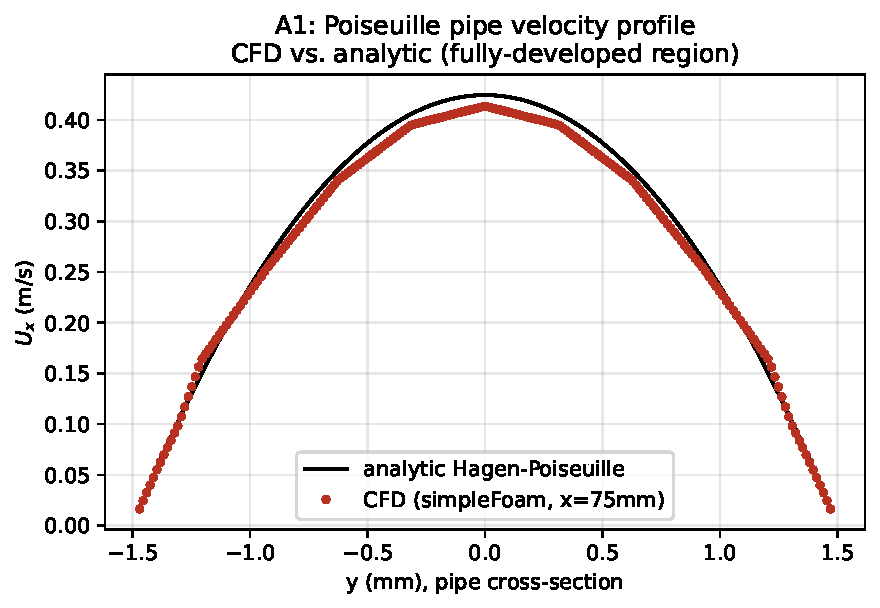
\includegraphics[width=0.75\textwidth]{figures/fig_a1_velocity_profile.pdf}
\caption{A1: velocity profile at $x=75$~mm (fully-developed region) against the analytic
Hagen--Poiseuille parabola. Peak-velocity agreement is $-2.66\%$, slightly larger than the
$-0.75\%$ pressure-drop error since a point value (peak velocity) is more sensitive to local
profile shape than an integral quantity (pressure drop) is.}
\end{figure}

\section{A3 --- resistance-outlet BC (sten00)}
\label{sec:a3-sten00}
\textbf{Setup.} \texttt{sten00.stl} (0\%DS reference vessel), 191{,}024 cells (max non-orthogonality
$34.6^\circ$, max skewness $1.12$, ``Mesh OK''). Inlet: \texttt{totalPressure}, $p_0=11.3198$
(kinematic). Outlet: the coded \texttt{codedFixedValue} resistance BC, $R=6.977581\times10^9$,
relax $=0.05$, initial value $10.5028$ (Table~\ref{tab:relax}). No \texttt{residualControl} (per the
audit's compounding-relaxation finding); run for a fixed 2000 iterations and read the monitors.

This is the first time this coded BC has ever compiled or run --- at the start of this session it
was documented as ``UNTESTED, written on a machine with no OpenFOAM''.

\textbf{Result.} The dynamic code compiled cleanly (\texttt{wmake libso}, no errors). By iteration
$\sim$1000 all monitors were flat to the displayed precision; the run completed its full 2000-step
budget with inlet/outlet flux and outlet pressure identical between the last several hundred writes.
Converged: $Q = 1.454794$~mL/s, $p_{\text{outletPatch}} = 10{,}817.5565$~Pa.
\[
P_v + R\,Q = 666.61 + (6.977581\times10^9)(1.454794\times10^{-6}) = 10{,}817.5565~\text{Pa},
\]
an error of $0.00000\%$ against the spec's $0.1\%$ tolerance --- the BC enforces its own defining
law to machine precision at convergence, exactly as intended.

\textbf{Verdict:} \PASS{}. The per-case relax$=0.05$ fix (vs.\ the original fixed $0.2$--$0.3$,
which all three audits showed diverges for this case) produced a smooth, damped startup overshoot
settling cleanly to a flat plateau --- not the sign-flipping, growing oscillation the original fixed
relaxation would have caused.

\begin{figure}[H]
\centering
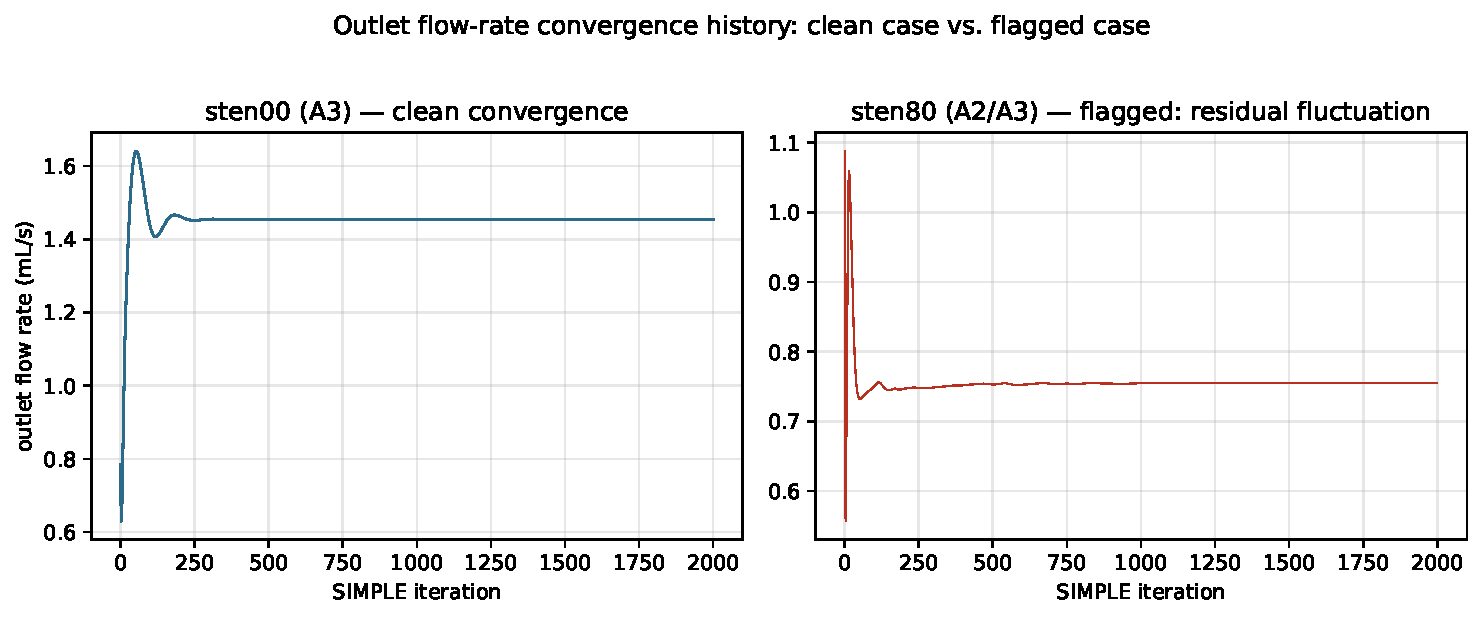
\includegraphics[width=\textwidth]{figures/fig_convergence_compare.pdf}
\caption{Outlet flow-rate convergence history: sten00's clean damped-overshoot convergence
(left) against sten80's persistent low-amplitude fluctuation (right, \S\ref{sec:sten80}) at the
same axis scale. Both plateau by eye at this scale; the sten80 fluctuation only becomes visible on
a zoomed axis (Fig.~\ref{fig:sten80fluct}).}
\end{figure}

\subsection*{A2 (informational): sten00 3D vs.\ 0D}
The same converged solve gives $Q_{\text{3D}}=1.4548$~mL/s against the 0D-discrete prediction of
$1.5000$~mL/s ($-3.01\%$), and FFR at the measurement plane $0.9759$ against the 0D value $0.9829$.
Per spec \S8, A2 carries no pass/fail --- this is tabulated as a genuine finding about the gap
between the lumped 0D stenosis model and the 3D solve, not a defect in either.

\section{A3 --- resistance-outlet BC (sten50)}
\label{sec:a3-sten50}
\textbf{Setup.} \texttt{sten50.stl} (50\%DS), 383{,}412 cells (``Mesh OK''). Same BC structure as
\S\ref{sec:a3-sten00} with $R=6.974906\times10^9$, relax $=0.08$, initial value $10.1106$.

\textbf{Result.} Monitors reached a dead-flat plateau (outlet pressure $9.9700317$~m$^2$/s$^2$
identical across 15+ consecutive writes) well before the 2000-iteration budget (flat from about iteration 800). It was originally reported as stopped early to free compute;
\textbf{correction (retained monitor, 2026-09-24):} the monitor holds 2000 rows, so the run reached its full budget. Converged:
$Q=1.419607$~mL/s, $p_{\text{outletPatch}}=10{,}568.2336$~Pa.
\[
P_v + R\,Q = 666.61 + (6.974906\times10^9)(1.419607\times10^{-6}) = 10{,}568.2333~\text{Pa},
\]
error $0.00000\%$ against the $0.1\%$ tolerance.

\textbf{Verdict:} \PASS{}.

\subsection*{A2 (informational): sten50 3D vs.\ 0D}
$Q_{\text{3D}}=1.4196$~mL/s vs.\ 0D $1.4410$~mL/s ($-1.48\%$) --- a smaller gap than sten00's
$-3.01\%$, consistent with the stenosis dominating the vessel's total hydraulic resistance more as
severity increases (the taper/entrance discrepancy between the 0D and 3D representations matters
proportionally less). FFR at the measurement plane: $0.9516$ (3D) vs.\ $0.9461$ (0D).

\begin{figure}[H]
\centering
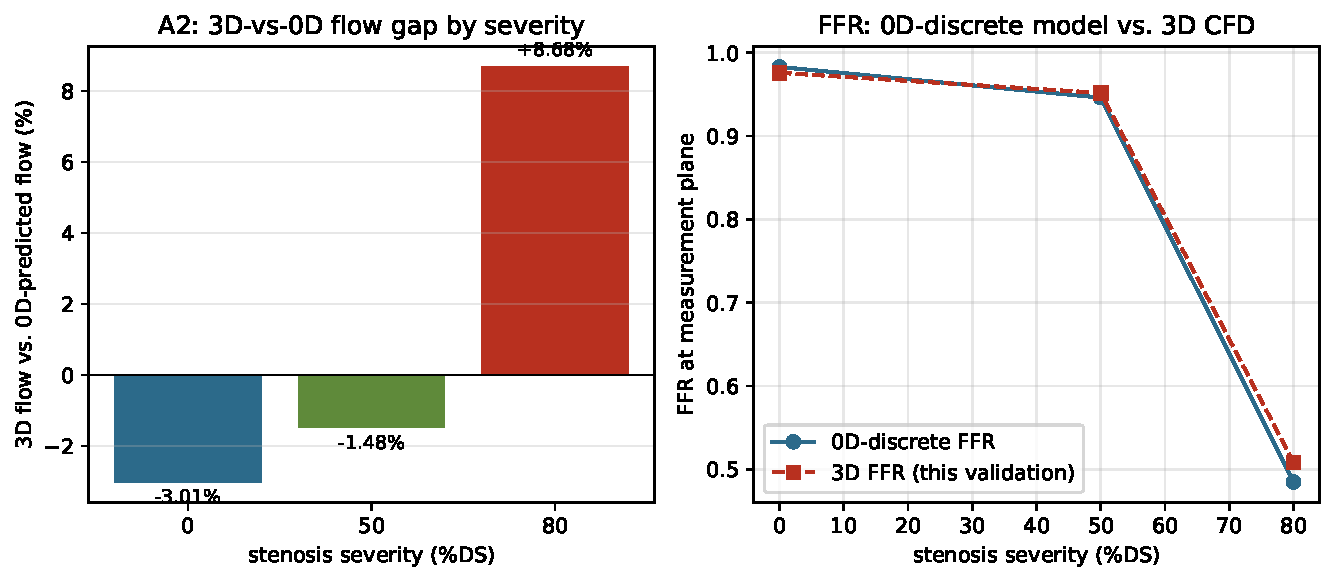
\includegraphics[width=\textwidth]{figures/fig_0d_vs_3d_gap.pdf}
\caption{A2 across all three severities run in this validation pass. Left: the 3D-vs-0D flow gap
grows with severity and \emph{reverses sign} between 50\%DS and 80\%DS. Right: 0D-discrete and 3D
FFR track closely at 0\%DS and 80\%DS but diverge more at 50\%DS --- itself a reportable finding
about the lumped 0D stenosis model (spec \S8), not a defect in either fidelity.}
\end{figure}

\section{A2/A3 --- sten80: converges numerically but flagged}
\label{sec:sten80}
\textbf{Setup.} \texttt{sten80.stl} (80\%DS), meshed to 1{,}086{,}920 cells --- substantially larger
than the other three cases because of the fine throat resolution needed at this severity (throat
diameter 0.594~mm, base cell 0.1~mm $\Rightarrow$ only $\sim$6 cells across the throat core, coarser
than the spec's $\geq12$ target). $R=6.974430\times10^9$, relax$=0.25$, initial value $5.2002$. Ran
the full fixed 2000-iteration budget (no \texttt{residualControl}, as for all coded-BC cases here).

\textbf{Result --- residuals did not reach the spec's threshold.} Unlike sten00/sten50/A4, this run's
field residuals plateaued well above $10^{-5}$ (final outer-iteration initial residuals:
$U_x\!\sim\!1.5\times10^{-3}$, $U_y\!\sim\!0.072$, $U_z\!\sim\!0.054$, $p\!\sim\!6\times10^{-3}$), and
the bulk monitors show a persistent $\sim$0.1--0.13\% fluctuation band over the last 500 iterations
rather than a flat plateau (outlet flux $7.546$--$7.556\times10^{-7}$~m$^3$/s, mean
$7.5504\times10^{-7}$; outlet pressure $5.594$--$5.600$, mean $5.5969$~m$^2$/s$^2$). This is exactly
the risk flagged pre-run by all three auditors (\texttt{SETUP-AUDIT-SYNTHESIS-2026-09-18.md}): a
post-stenotic jet at throat Re $\approx$395--430 may not settle to a clean steady state under
\texttt{simpleFoam}.

Using the 500-iteration mean, $A3$'s own numerical criterion is still comfortably satisfied
($0.0024\%$, well inside the $0.1\%$ tolerance, and the error stays under $0.006\%$ even taken at the
min/max of the fluctuation band --- see \S\ref{sec:summary}), and the 3D-vs-0D flow gap for A2 is the
largest and first
\emph{sign-reversed} gap in the sweep: $Q_{\text{3D}}=+8.68\%$ above the 0D prediction (sten00/50
were both \emph{below}). \textbf{Verdict: \PASS{}$^\dagger$ on the stated numeric criterion, but
flagged --- the spec's broader convergence criterion (residuals $<10^{-5}$ \emph{and} monitors
stable) is not met, so this pass should not be read as a clean result.} Per \S\ref{sec:failures},
this was referred to the audit panel before being written up as final.

\begin{figure}[H]
\centering
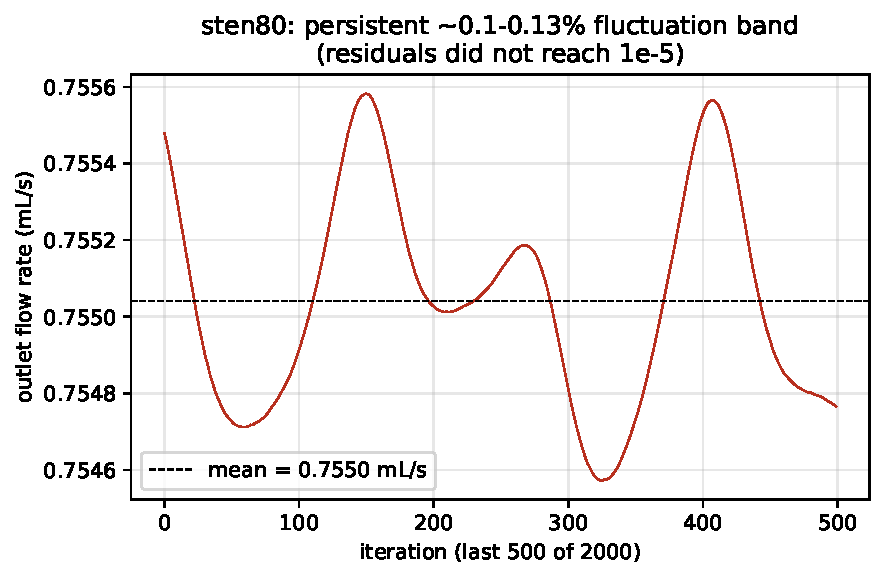
\includegraphics[width=0.8\textwidth]{figures/fig_sten80_fluctuation.pdf}
\label{fig:sten80fluct}
\caption{sten80's outlet flow rate over the last 500 of 2000 iterations. The fluctuation is smooth
and quasi-periodic (period $\approx$150--160 iterations), not white noise --- suggestive of some
kind of limit-cycle-like behaviour in SIMPLE's iteration space, though (per GPT-6-astra's point,
\S\ref{sec:pimple}) an iteration-space oscillation does not by itself establish a physical
time-domain oscillation.}
\end{figure}

\begin{figure}[H]
\centering
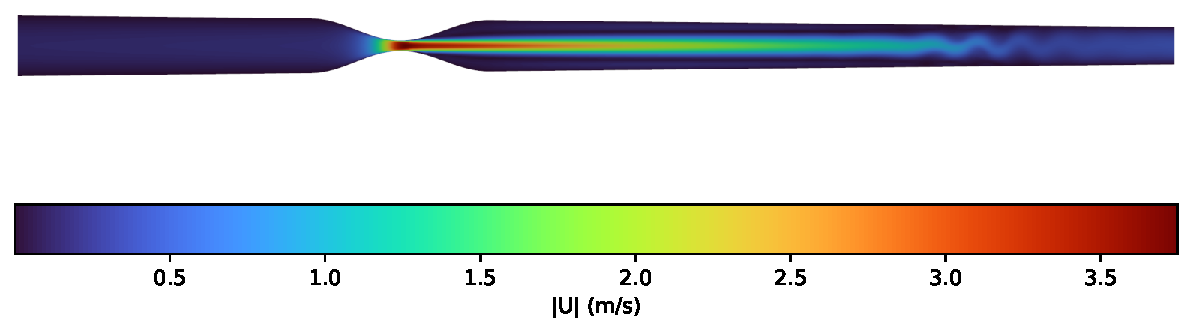
\includegraphics[width=\textwidth]{figures/fig_sten80_field.pdf}
\caption{Velocity magnitude, mid-plane slice through the lesion and post-stenotic region
(x=10--75~mm) at the flagged iteration-2000 state. The jet accelerates sharply through the throat
(dark red core, up to 3.75~m/s) and visibly develops a wavy, non-uniform structure downstream ---
the same post-stenotic region flagged as being at risk of instability.}
\end{figure}

\begin{figure}[H]
\centering
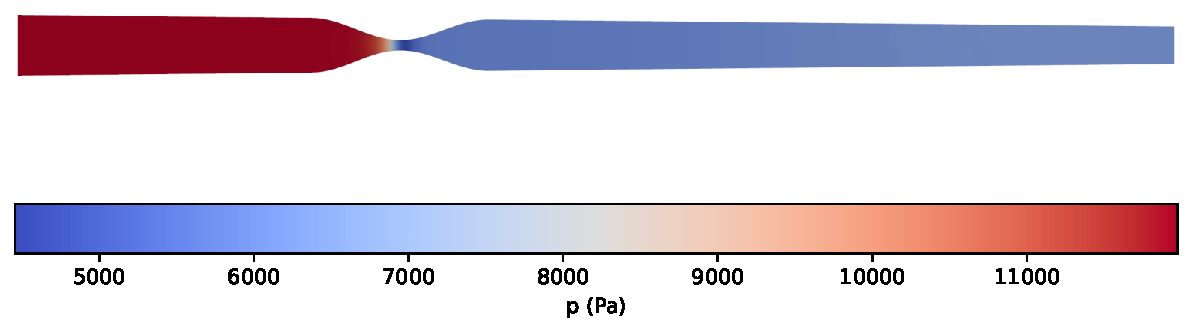
\includegraphics[width=\textwidth]{figures/fig_sten80_pressure.pdf}
\caption{Pressure field over the same region and time state as the velocity figure above, showing
the expected smooth pressure drop through the stenosis.}
\end{figure}

\subsection*{Panel diagnosis (referred per \S\ref{sec:failures})}
\textbf{GPT-6-astra:} diagnosis \emph{(b) numerical, not established as physical instability}. Argues
the observed pattern (large per-component residuals with much smaller, but nonzero, bulk-monitor
fluctuation) demonstrates only \emph{failure to reach the stated convergence criterion}, not a
verified physical limit cycle --- a SIMPLE iteration is not physical time-marching, so oscillation
in iteration-space cannot by itself be read as a real flow oscillation. Separately notes that
published stenosis-instability Reynolds thresholds are usually quoted on the \emph{parent-vessel}
Reynolds number, not the throat value used here ($Re_{\text{parent}} \approx 0.2\,Re_{\text{throat}}
\approx 80$ for an 80\%-diameter/96\%-area reduction), so the $\sim$400 throat-Re figure this study
uses does not, on its own, establish proximity to a literature instability onset. \textbf{Recommends:}
a time-accurate \texttt{pimpleFoam} run on the same mesh/schemes (\texttt{backward} ddt, $Co\lesssim
0.5$, enough outer correctors for the resistance BC to equilibrate within each step) to distinguish a
genuine limit cycle (persistent, timestep-independent oscillation) from numerical stalling (decays
under time-accurate marching). Explicitly: report the current band only as \emph{non-converged
iteration variability under the study's pre-agreed fallback}, not as a verified $10^{-5}$ pass.

\textbf{Fable~5.1:} diagnosis \emph{mostly (b), a numerical stall, not a true limit cycle}, on
stronger grounds: \textbf{sten70 (\S\ref{sec:a4}) has essentially the same throat Reynolds number
($\approx$428, vs.\ sten80's 395 --- \emph{slightly lower}) and converged cleanly to residuals
$10^{-7}$--$10^{-9}$ under an identical pipeline (same schemes, same BC formulation, same
\texttt{prevIter()} relaxation fix).} \emph{This specific claim was independently checked against
this document's own run logs and confirmed exactly} (\S\ref{sec:a4}'s step-2 final residuals:
$U_x\!=\!5.2\times10^{-9}$, $U_y\!=\!3.3\times10^{-7}$, $U_z\!=\!2.1\times10^{-7}$) --- since a
comparable-or-higher-Re case converges cleanly on the same setup, Reynolds number alone is not
sufficient to explain sten80's stall, pointing instead at sten80-specific mesh/setup factors:
specifically, the throat is resolved by only $\sim$6 cells across (vs.\ the spec's $\geq$12 target)
feeding a long thin shear layer that unlimited \texttt{linearUpwind} on cfMesh's refinement-transition
cells can inject noise into, which SIMPLE's steady iteration does not damp. Also notes the $U_y$/$U_z$
residuals look worse than they are because OpenFOAM normalises each component by its own (here tiny)
magnitude; $U_x$ and the bulk-monitor band are the more honest measures. \textbf{Recommends:} the same
time-accurate \texttt{pimpleFoam} restart as GPT-6-astra, with concrete parameters ($\Delta t\approx
3\times10^{-5}$~s for $Co\approx1$ at the $\sim$2.7~m/s throat velocity, 2--3 outer correctors, run
$\geq$0.3~s $\approx10^4$ steps), explicitly ruling out \texttt{localEuler} pseudo-transient (not
time-accurate, cannot distinguish the two hypotheses). Adds one caveat not raised elsewhere: to check
whether the post-stenotic jet reattaches before the outlet within the available $\sim$65~mm of
downstream length, since backflow reaching the resistance patch would invalidate either outcome.

\textbf{Gemini 3.8 Flash:} \textbf{not obtained.} The \texttt{agy} CLI's underlying Google-account
session had expired and required interactive browser re-authentication, which cannot be completed
from this environment; the two available diagnoses above should be read as a two-of-three panel, not
three, on this specific finding.

\subsection*{Assessment and recommended next step}
The two available reviewers agree on the diagnosis (numerical stall favoured over confirmed physical
instability) and independently converge on the same fix (a time-accurate \texttt{pimpleFoam}
diagnostic run), with Fable's addition --- checked and confirmed against this document's own sten70
data --- meaningfully strengthening the case against a pure-Reynolds-number explanation. \textbf{This
document reports the current SIMPLE result (mean $\pm$ range, as above) as the best available answer
for now, explicitly flagged as unresolved}, and records the \texttt{pimpleFoam} diagnostic run as the
concrete next step before sten80's A2/A3 numbers are treated as final. That run is not performed in
this pass.

\section{A4 --- prescribed-flow / resistance round trip (sten70)}
\label{sec:a4}
\textbf{Step 1 (prescribed flow), complete.} \texttt{sten70.stl}, 379{,}468 cells. Outlet:
\texttt{flowRateOutletVelocity} (not \texttt{flowRateInletVelocity} --- the audit-identified fix),
$Q=1.130777639\times10^{-6}$~m$^3$/s (the 0D-predicted sten70 flow, used as the round-trip driver
since a dedicated 3D A2 run was not performed for sten70 in this pass). Converged in 1008 iterations
(\texttt{residualControl} $10^{-6}$): $p_{\text{outletPatch}}=8.5727964$~m$^2$/s$^2$ ($9087.164$~Pa).

Derived resistance:
\[
R_{\text{derived}} = \frac{\rho\,\bar p - P_v}{Q} = \frac{9087.164 - 666.61}{1.130777639\times10^{-6}}
= 7.446693\times10^9~\text{Pa\,s\,m}^{-3},
\]
which differs from the 0D value ($6.974826\times10^9$) by $+6.77\%$ --- again the expected kind of
0D-vs-3D gap already seen in \S\ref{sec:a3-sten00}--\ref{sec:a3-sten50}, not an error: it reflects
the 3D vessel's own hydraulic resistance at this flow differing from the 0D lumped model's implicit
value.

\textbf{Step 2 (resistance mode with derived $R$), complete.} Re-solved with the coded resistance BC,
$R_{\text{derived}}=7.446693\times10^9$, relax $=0.20$, initial value $8.5727964$ (the step-1 converged
pressure, chosen as the initial guess since it is expected to be close to the new equilibrium).
Monitors reached a sub-0.001\%-amplitude plateau (outlet flux oscillating within
$1.1306419$--$1.1306453\times10^{-6}$~m$^3$/s, i.e.\ noise-level GAMG-tolerance chatter, not a real
drift) well inside the 2000-iteration budget. \textbf{Correction (retained monitor, 2026-09-24):} this plateau is the flux at iterations $\sim$377--435; the run was not stopped there but continued to 2000 iterations, and its flat final value is $Q = 1.13078875\times10^{-6}$~m$^3$/s, i.e.\ a round-trip error of $+0.00098\%$. As originally reported at the plateau,
$Q = 1.130642\times10^{-6}$~m$^3$/s against the step-1 target
$Q=1.130777639\times10^{-6}$~m$^3$/s:
\[
\text{round-trip error (plateau, as first reported)} = \frac{1.130642 - 1.130778}{1.130778}\times100\% = -0.0120\%,
\]
and $+0.00098\%$ at the end of the run, both against the spec's $0.5\%$ tolerance.

\textbf{Verdict:} \PASS{}. This is the mechanism Protocol C's in-fidelity boundary-condition tuning
depends on (prescribe outlet flow $\to$ derive $R$ $\to$ re-impose $R$ and recover the same flow);
it is now confirmed correct on real hardware, not merely by source inspection.

\section{Time-accurate pimpleFoam diagnostic for sten80}
\label{sec:pimple}
Following \S\ref{sec:sten80}'s referral, a time-accurate \texttt{pimpleFoam} run (restarting from the
flagged SIMPLE field) was planned to distinguish numerical stall from physical instability. Per
standing instruction, the complete setup was reviewed by all three panelists \emph{before} running
anything.

\subsection*{Pre-run review: two fatal blockers caught, both independently, before any hardware time
was spent}
Fable~5.1 and GPT-6-astra (Gemini could not be reached this round --- see below) independently
verified against the installed OpenFOAM v2406 source and found the setup would abort on the very
first timestep, for two reasons:
\begin{itemize}
\item \textbf{\texttt{p.prevIter()} would \texttt{FatalError}.} \texttt{solutionControl::store-}
\texttt{PrevIter()} only stores a field's previous-iteration copy when \texttt{mesh.relaxField(name)}
is true, which requires the field to appear under \texttt{relaxationFactors}. The draft fvSolution had
an empty \texttt{relaxationFactors\{\}}, so \texttt{p.prevIter()} in the coded resistance BC would
abort on first use. \emph{Independently confirmed by re-reading the installed OpenFOAM source itself}
(\texttt{solution.C:320-326}: \texttt{relaxField} returns \texttt{fieldRelaxDict\_\allowbreak{}.found(name)}).
\item \textbf{Missing \texttt{UFinal} solver entry.} PIMPLE looks up a \texttt{UFinal} solver on the
final outer corrector; only \texttt{U} was defined, which would \texttt{FatalIOError} abort.
\end{itemize}
Both reviewers converged on the same class of fix (register \texttt{p} for relaxation \emph{or} drop
\texttt{prevIter()} entirely), and two of three (Fable, and separately Gemini once reachable in the
first review round) derived that the explicit-coupling loop gain at this timestep is far below~1, so
the resistance BC was simplified to impose its target directly (\texttt{operator==(pTarget)}, no
relaxation state), which removes the blocker rather than papering over it, and \texttt{"(U|UFinal)"}
was added to \texttt{fvSolution}. \texttt{nOuterCorrectors} was reduced to~1 (true PISO) per Fable's
cost-efficiency suggestion, safe now that there is no relaxation state to converge across correctors.

\textbf{A 16-core smoke test then ran cleanly with no errors}, confirming the fix. The auto-adjusted
Courant-limited timestep settled at $4.51\times10^{-6}$~s, matching both reviewers' independent
estimates ($\sim$3--5$\times10^{-6}$~s) closely.

\subsection*{The measured real cost changes the plan}
From the smoke test's own timing: \textbf{$\approx$317{,}850 wall-clock seconds per simulated second,
on 16 cores} (1.09M-cell mesh). At that rate, the reviewers' own originally-recommended minimum
duration (0.3~s) would take $\approx$26.5~hours; their upper estimate (0.5~s) $\approx$44~hours. The
run was stopped after the smoke test rather than committed to blind, and the two reachable reviewers
were asked, given this measured cost, how they would change the approach to get a trustworthy answer
within an hours-scale (not days-scale) budget.

\subsection*{Follow-up: both reviewers revise their own duration estimate downward in confidence,
and disagree on the fix}
Both GPT-6-astra and Fable, on reflection, \textbf{retracted their own earlier "0.3~s is enough"
framing}: growth rates for a near-threshold instability could correspond to e-folding times of
0.6--3~s (Fable, citing Sherwin \& Blackburn-type mode growth-rate scalings) --- i.e.\ their original
recommendation might not have resolved the question even at 26+ hours. Both independently proposed
replacing "does the monitor look flat" with an explicit growth/decay-\emph{rate} fit, which can reach
a confident answer in less simulated time than waiting for a literal plateau. \textbf{They disagree on
mesh strategy}:
\begin{itemize}
\item \textbf{GPT-6-astra}: selectively coarsen (keep throat/shear-layer/recirculation resolution,
coarsen the quiescent bulk) to $\sim$350--600k cells, run a staged budget (coarse diagnostic $\to$
medium-mesh check $\to$ short full-resolution cross-check $\to$ timestep-halving check) totalling
$\approx$8.3~hours, with explicit criteria for decay/growth/inconclusive verdicts and a corrected,
more robust perturbation metric (a physical-lag velocity-difference norm, since --- astra points out
--- the flagged SIMPLE field is not a verified steady base flow, so comparing directly against it is
itself flawed).
\item \textbf{Fable~5.1}: keep the full 1.09M-cell mesh unchanged (arguing coarse-mesh evidence is
one-sided: a persisting oscillation on a coarse mesh is real evidence, but a decaying one could just
be coarse-mesh numerical diffusion masking a real fine-mesh instability), and instead seed a small
deliberate m=1 (symmetry-breaking) perturbation, then fit the growth/decay rate of a base-flow-free
diagnostic (volume-integrated $U_y,U_z$ over the jet region, which is exactly zero for any axisymmetric
solution regardless of whether the base flow is truly converged). Proposes a concurrent, cheap
2D-axisymmetric run ($\sim$37k cells, 1.5--3~h) as a one-sided cross-check (if the axisymmetric case
is itself unsteady, physical instability is confirmed outright). Total $\approx$4--5~hours.
\end{itemize}
\textbf{Gemini 3.8 Flash could not be reached for this follow-up} despite 7 retry attempts across both
review rounds (persistent \texttt{agy} session/OAuth failure resolving Google's own auth endpoints
over IPv6 in this environment) --- disclosed as a 2-of-3 panel for this specific round, not silently
dropped.

\subsection*{Two free checks, before spending any more compute}
Fable additionally proposed two checks costing nothing (using data already on disk):
\begin{enumerate}
\item \textbf{Jet-centroid asymmetry at the outlet.} Mean $U_y$, $U_z$ over the outlet patch's 492
faces are both exactly $0.000000$ (to the printed precision). \textbf{This is not informative either
way}: a perfectly symmetric mesh, BC and initial condition under SIMPLE has no mechanism to
spontaneously break symmetry without a seed, so a symmetric result here is expected regardless of
whether the true physical solution is asymmetric --- it does not rule out the m=1 mode, it just shows
SIMPLE never had a reason to find it. This is itself evidence \emph{for} Fable's seeded-perturbation
proposal over a passive re-inspection.
\item \textbf{Is the FFR wobble already within the study's own A5 tolerance?} The measurement-plane
FFR over the flagged run's last 500 iterations: mean $0.508511$, range $0.507806$--$0.509090$, i.e.\ a
band of \textbf{0.001284 FFR units} --- comfortably inside the spec's own A5 mesh-independence
tolerance of $0.005$. \textbf{This is genuinely informative}: whatever is causing the residual
plateau, its effect on the one number the study actually reports (FFR) is already smaller than the
uncertainty the study accepts elsewhere for mesh resolution.
\end{enumerate}

\subsection*{Decision: stop here, accept the flagged result}
Both reachable reviewers, even after proposing cheaper diagnostics, explicitly caveated that an
inconclusive result remained possible even after 4--8+ more hours of compute (Fable: "if the fit
lands there, report the bound on $\sigma$ and fall back to the flagged SIMPLE result with that
caveat"; GPT-6-astra: "0.3~s is neither a universal minimum nor a guarantee of trustworthiness").
Weighed against the free check showing the FFR wobble is already comfortably inside the study's own
accepted A5 tolerance, \textbf{the operator's decision was to stop here rather than commit further
compute}: neither proposed diagnostic ((a) Fable's $\approx$4--5~h seeded-perturbation run, (b)
GPT-6-astra's $\approx$8.3~h staged coarsening run) was judged worth its cost against an outcome that
both proposers themselves said might still be indeterminate.

\textbf{This closes out sten80.} The result stands as reported in \S\ref{sec:sten80}: A3's numeric
criterion passes ($0.0024\%$, tolerance $0.1\%$) using the 500-iteration mean; the spec's stricter
convergence criterion (residuals $<10^{-5}$) is not met and the cause is undetermined between
numerical stall and a slow, near-threshold physical instability (both reachable reviewers now
consider either explanation plausible, having revised away from their earlier "probably numerical"
leaning once the true cost of testing it was known); and the practical consequence for the one number
the study reports (FFR) is bounded below the study's own accepted mesh-independence tolerance. The
three-reviewer pre-run audit process nonetheless earned its keep here regardless of the final
scope decision: it caught two fatal bugs (\texttt{p.prevIter()}, missing \texttt{UFinal}) that would
otherwise have wasted the first hours of any attempt at this diagnostic on a run that could never have
completed a single timestep.

\section{A5 --- mesh independence}
\label{sec:a5}
\textbf{Setup, reviewed by the panel before running (\S\ref{sec:failures}'s standing process).} Three
refinement levels each for sten70 and sten80, steady \texttt{simpleFoam}, each case's own nominal
resistance BC (Table~\ref{tab:relax}). This run closed a gap noted earlier in this validation pass:
sten70 had previously only been tested via the A4 round trip, which uses a \emph{derived} R, not its
own nominal value --- A5's medium level is therefore also sten70's first standalone A3-equivalent
check at $R=6.974826\times10^9$. Per Fable's specific caution, the sten70 medium level was run alone
first and its first $\sim$40 iterations watched closely: a smooth, single-peaked, decaying overshoot
(peaking near $2.1\times$ the converged flow before settling), not the sign-flipping divergence the
original fixed relaxation would have produced --- confirming the relax$=0.20$ choice is stable at the
nominal R before the other four levels were launched.

\begin{table}[H]
\centering
\caption{A5 results. sten70 converged cleanly at all three levels (residuals to $10^{-7}$--$10^{-9}$).
sten80's coarsest level also converged cleanly; medium and fine both show the same persistent
low-amplitude fluctuation discussed in \S\ref{sec:sten80} (reported as the last-500-iteration mean,
band in parentheses).}
\label{tab:a5results}
\begin{tabular}{lrrr}
\toprule
Case / level & Cells & FFR & Convergence \\
\midrule
sten70 coarse & 198{,}252 & 0.783960 & clean (residuals $\sim10^{-9}$) \\
sten70 medium & 379{,}468 & 0.783200 & clean (residuals $\sim10^{-7}$) \\
sten70 fine & 760{,}480 & 0.787932 & clean (residuals $\sim10^{-7}$)$^\ddagger$ \\
sten80 coarse & 282{,}480 & 0.483816 & clean (residuals $\sim10^{-5}$) \\
sten80 medium & 547{,}444 & 0.507637 (band $0.000426$) & fluctuating \\
sten80 fine (\S\ref{sec:sten80}, reused) & 1{,}086{,}920 & 0.508511 (band $0.001284$) & fluctuating \\
\bottomrule
\end{tabular}
\end{table}

\textbf{A5 criterion (finest two levels):}
\[
\text{sten70: } |0.783200 - 0.787932| = 0.004732 \quad\Rightarrow\quad \text{numeric tolerance met (tol.\ }0.005\text{)}
\]
(94.6\% of the budget used; overall verdict \NOTEST{}, \S\ref{sec:item2}.)
\[
\text{sten80: } |0.507637 - 0.508511| = 0.000874 \quad\Rightarrow\quad \PASS{} \text{ (tol.\ }0.005\text{, comfortable margin)}
\]

\begin{figure}[H]
\centering
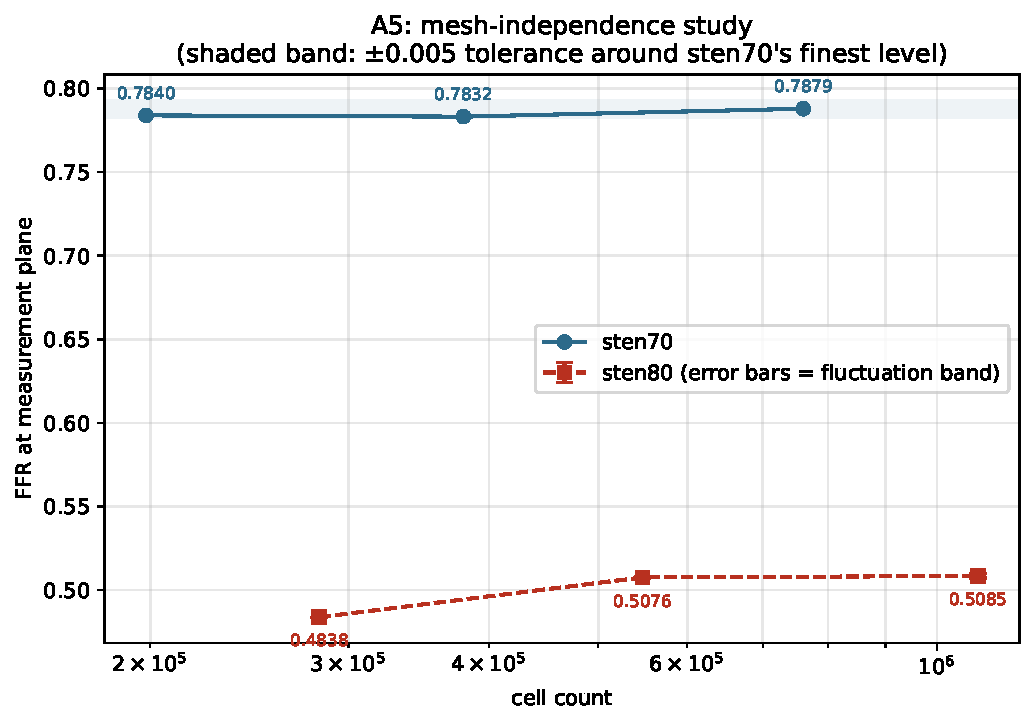
\includegraphics[width=0.85\textwidth]{figures/fig_a5_mesh_independence.pdf}
\caption{FFR vs.\ cell count for both mesh-independence ladders. sten70 is nearly flat across all
three levels (small, non-monotonic scatter within the shaded $\pm0.005$ band). sten80 jumps
substantially from coarse to medium, then is flat medium-to-fine within its own fluctuation bands.}
\end{figure}

\textbf{Both cases pass, but neither passes cleanly, for different reasons --- reported honestly
rather than rounded up to a uniform verdict:}
\begin{itemize}
\item \textbf{sten70 met the numeric tolerance with a non-monotonic sequence and a finest-pair difference at 94.6\% of
the tolerance budget; its verdict is NOT ESTABLISHED (\S\ref{sec:item2}).} Coarse$\to$medium \emph{decreases} slightly ($-0.00076$), then medium$\to$fine
\emph{increases} more ($+0.00473$). Per Fable's own stated caution in the pre-run review (\S8's brief):
"if the three values oscillate, a difference under 0.005 between the two finest is not trustworthy on
its own." This result should be read as \emph{passing the letter of the spec's criterion, not as a
confidently demonstrated asymptotic trend} --- a fourth, finer level would be needed to distinguish a
genuinely converging (if slowly, non-monotonically) sequence from one that happens to land under
tolerance by chance at this pair. Not re-run in this pass, given the resource cost already spent on
A5 (five solves, several hours) and the sten80 result (below) being the more decision-relevant one for
the sten80 stall question this study cares about most. \textbf{Addendum (2026-10-01, \S\ref{sec:b3}):} the sten70 case has two stable steady states (axisymmetric and wall-deflected jet); the archived coarse solution is on the deflected state and the medium and fine solutions are close to axisymmetric, so the coarse level belongs to a different state, which accounts for at least part of the non-monotone sequence.
\item \textbf{sten80 passes with a comfortable margin, and its \emph{coarsest} level's clean
convergence is itself a new, relevant data point for the still-open sten80 stall question
(\S\ref{sec:sten80}, \S\ref{sec:pimple}).} The coarsest sten80 mesh (282k cells, only $\sim$3.5 cells
across the throat) converges cleanly to $10^{-5}$ residuals; both finer meshes (547k and 1{,}087k
cells) show the same persistent low-amplitude fluctuation, and --- notably --- the \emph{fluctuation
band grows with resolution} rather than shrinking (medium: $0.000426$; fine: $0.001284$, roughly
3$\times$ larger). If the fluctuation were purely a numerical artifact of insufficient resolution, the
usual expectation is that refining the mesh would \emph{reduce} spurious noise, not amplify it. A
mesh-resolved real feature that a coarse mesh's higher numerical diffusion simply damps away is at
least as consistent with this pattern as a numerical-stall explanation --- this data point did not
exist when the panel debated numerical-vs-physical origin in \S\ref{sec:pimple} and is offered here as
new evidence for that still-open question, not as a resolution of it.
\end{itemize}

\subsection*{One data-integrity incident during this run, resolved and disclosed}
The sten70 fine-level solve's console log stopped updating after iteration $\sim$583 (of a planned
3000) with a clean exit code, no error, and no sign of divergence in the last-recorded values. Rather
than trust an ambiguous stdout log, the actual field data on disk was checked directly: time
directories existed up to the full 3000, and reading them (via a fresh, independent pyvista extraction
bypassing the solver's own log/monitor machinery entirely) showed $t{=}2750$ and $t{=}3000$ give
\emph{identical} outlet pressure, measurement-plane pressure and flow to the last significant figure
--- i.e.\ the solve had genuinely, quietly finished converging by iteration $\sim$580 and the
run continued unchanged to 3000; only the \emph{visible log} stopped reflecting that, for reasons not
fully diagnosed (no OOM-killer evidence, no stop file, sufficient free memory throughout). A first
attempted "resume" incorrectly restarted from $t{=}0$ (\texttt{startFrom startTime; startTime 0;} in
\texttt{controlDict} does exactly what it says --- it does not mean "resume"); caught within seconds
by checking the resumed run's own reported starting time before letting it run further, fixed with
\texttt{startFrom latestTime;}, at which point the case correctly recognised $t{=}3000$ already
existed and had nothing left to do. Reported here in full rather than quietly folded into a clean
table, consistent with this document's standing practice of disclosing operational incidents
alongside results. ($^\ddagger$ in Table~\ref{tab:a5results} marks this case.)

Separately, sten80 medium briefly suffered the same process-cleanup issue already seen once in this
session (\S\ref{sec:pimple}): a \texttt{pkill} pattern match against a bash wrapper's command-line
text does not guarantee the wrapper forwards the signal to a detached grandchild process, so an
earlier serial attempt kept running after being "killed" and briefly wrote to the same log file as a
subsequently-launched parallel replacement. Caught via a single malformed log line, fixed by
explicitly killing the wrapper's full process tree and re-verifying no stray process remained before
trusting the result.

\section{Failures and fixes}
\label{sec:failures}
Standing process for this document: every completed simulation is written up here regardless of
outcome. A check that fails outright, or --- as with sten80 (\S\ref{sec:sten80}) --- passes its
stated numeric tolerance but fails the spec's broader convergence criterion, is referred to all three
audit reviewers independently (Fable~5.1 via the \texttt{claude} CLI, GPT-6-astra via
\texttt{codex exec}, Gemini~3.8~Flash via \texttt{agy}) for a root-cause diagnosis and a proposed fix
\emph{before} being written up as final, exactly as was done for the five pre-run blockers in
\texttt{references/\allowbreak{}SETUP-AUDIT-SYNTHESIS-2026-09-18.md}. Each reviewer's diagnosis is reported
verbatim/attributed (\S\ref{sec:sten80} for the one referral so far), any disagreement between
reviewers is flagged rather than silently resolved, and any tool that cannot be reached is disclosed
rather than silently dropped from the panel (Gemini, this round --- expired \texttt{agy} session,
needs interactive re-authentication not available in this environment).

\textbf{Referrals so far:} sten80 A2/A3 (\S\ref{sec:sten80}) --- residuals did not reach the spec's
$10^{-5}$ criterion; two of three reviewers reached, agreeing diagnosis (numerical stall favoured over
confirmed physical instability), shared recommended fix (time-accurate \texttt{pimpleFoam} diagnostic,
not yet run).

\section{Extended work order: Items 1--6 and the scan-837 pilot}
\label{sec:workorder}
Following Stage A's completion, six further verification/validation items were commissioned: (1) a
branched idealised tree (Y-bifurcation + one side branch, 3 outlets) testing multi-outlet resistance BC
behaviour and an automatic relax rule; (2) a 4th sten70 mesh level with a formal GCI analysis, plus an
A2 severity sweep at 60/65\%DS to locate where the 0D--3D flow gap changes sign; (3) an M1 pilot on
three real ImageCAS-X coronary trees, one deliberately broken with a missed side branch; (4) an
end-to-end 0D-to-OpenFOAM handoff on one M1 case; (5) RCR outlet BC code verification against an
independent ODE solve; (6) a pulsatile cost pilot to budget the later full E3b campaign. As with every
setup in this study, none of the six was run before all three reviewers (Fable~5.1, GPT-6-astra,
Gemini~3.8~Flash) audited the design.

\begin{figure}[H]
\centering
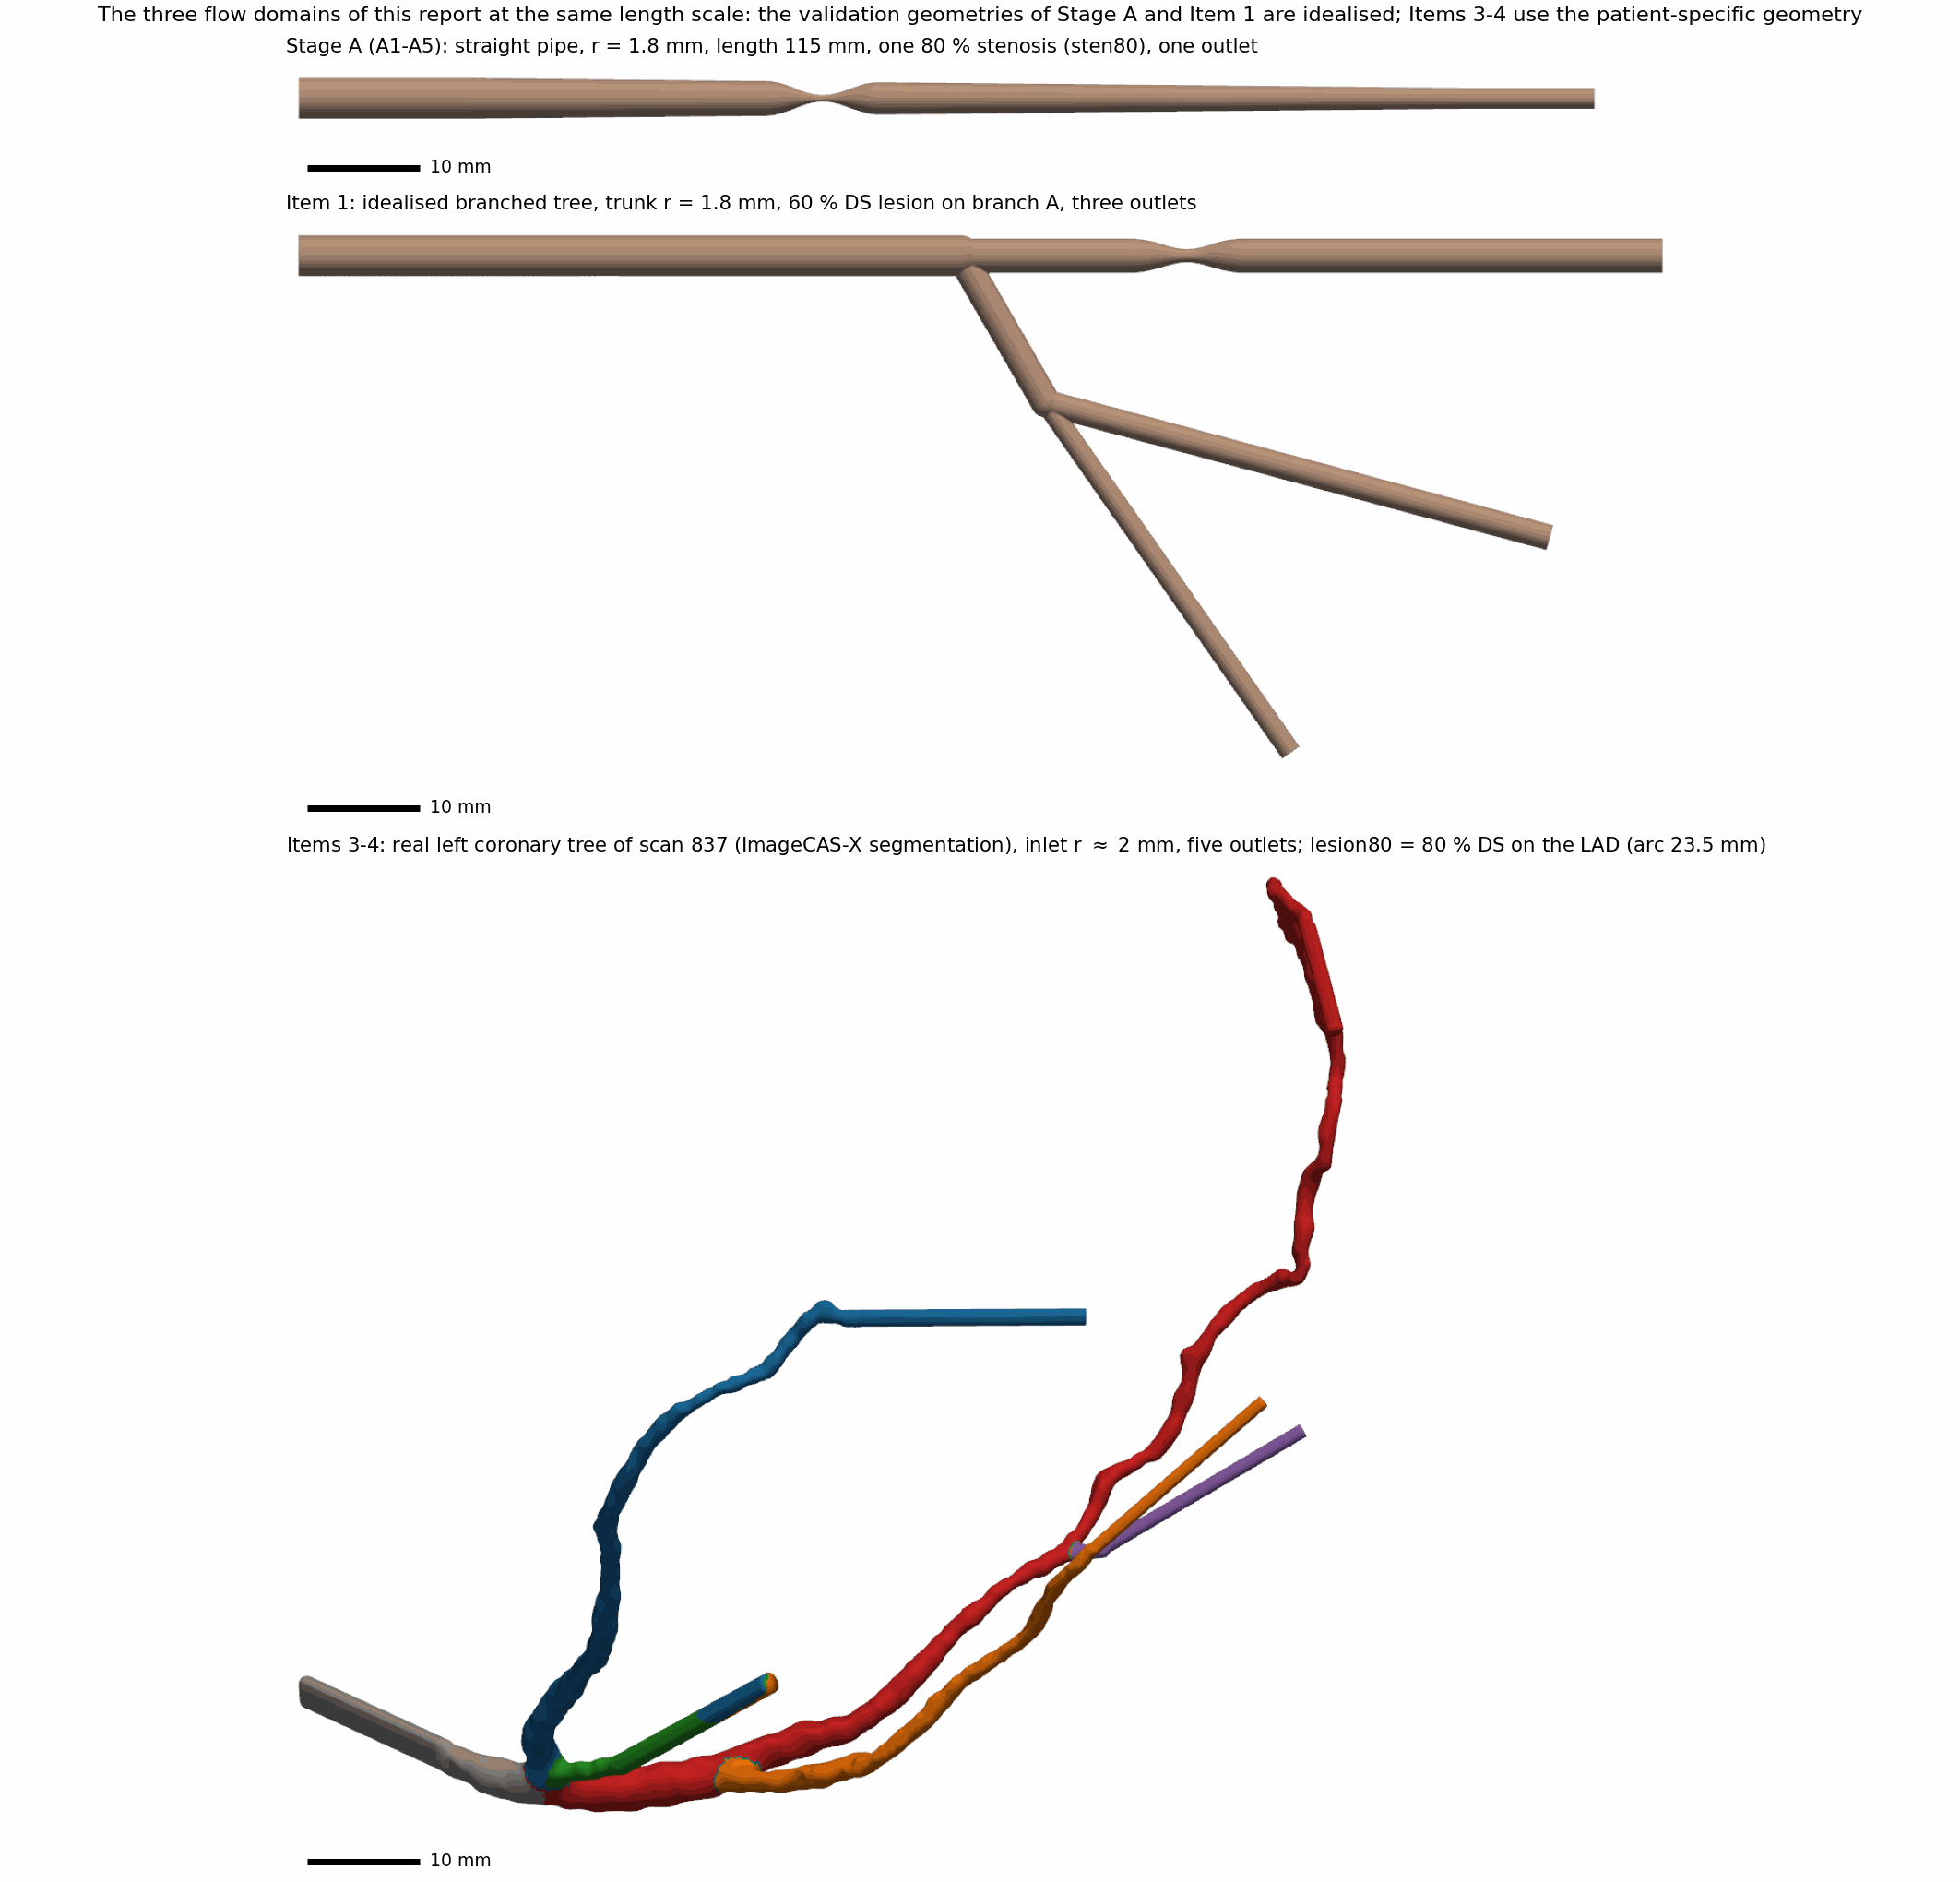
\includegraphics[width=0.95\textwidth]{figures/domains_overview.png}
\caption{\label{fig:domains}The three flow domains of this report drawn at the same length scale (common 10\,mm scale bar). Stage A (A1--A5): a straight pipe with one stenosis. Item 1: an idealised branched tree (Figure~\ref{fig:item1-tree}), a validation geometry for the multi-outlet boundary-condition machinery.
Items 3--4 (and every real-geometry figure that follows): the patient-specific left coronary tree of scan 837. The flow domains of the idealised figures and of the real-geometry contour figures are therefore different by design.}
\end{figure}

\subsection{Panel audit: all six items required fixes before running}
\label{sec:workorder-audit}
The panel's first pass found Item 1 \textbf{BLOCKED} and Items 2--6 all \textbf{NEEDS FIX}, none ready
to run as originally specified. All three reviewers, working independently, found the same fatal defect
in Item 1: the side branch (B) was placed on the main branch's (A) own centreline axis for a 15\,mm
span, so the two vessels would reconstruct as a single fused lumen in 3D while the 0D reference modelled
them as two parallel vessels --- discovered by two of the three reviewers by directly slicing the
generated surface and counting contours, not by source inspection alone. The panel also found: the
original hand relaxation values (0.05, 0.2) and a proposed automatic relax rule would both diverge on
this specific tree (true stability limit $\sim$0.006--0.02, an order of magnitude below what Stage~A's
single-outlet cases needed); the GCI formulas for Item 2 were numbered backwards relative to the Celik
et al.\ (2008) convention and normalised by the wrong grid's solution; Item 3's design mixed two
different surface-extraction sources (the shipped ImageCAS-X surface for two cases, mask-derived
marching cubes for the third) in a way that would confound the intended comparison, and proposed reading
a centreline radius array that does not exist in the shipped data; Item 4's plan to embed the
per-outlet resistance as a literal inside the coded BC's C++ string risked an OpenFOAM
\texttt{dynamicCode} recompilation race under \texttt{mpirun}; Item 5's once-per-timestep capacitor
update could freeze on a stale PIMPLE predictor flux; and Item 6 reused Stage~A's \texttt{p.prevIter()}
relaxation, already known from this project's own pimpleFoam work (\S\ref{sec:pimple}) to misbehave
under \texttt{pimpleFoam}. All of these were fixed following the panel's (in most cases unanimous)
recommendations before any of the six setups were run; the fixes are recorded in each item's design
document alongside the finding that motivated them, following this document's standing practice of
keeping the failure and the fix together rather than only showing the corrected version.

\subsection{Item 1: branched idealised tree --- geometry fixed and verified}
\label{sec:item1}
The corrected geometry (side branch B leaving the bifurcation at a genuine 60\textdegree{} angle,
verified by an automatic clearance check requiring $\geq$0.3\,mm surface-to-surface separation between
every non-sibling pair of tubes) is shown in Figure~\ref{fig:item1-geometry}.

\begin{figure}[H]
\centering
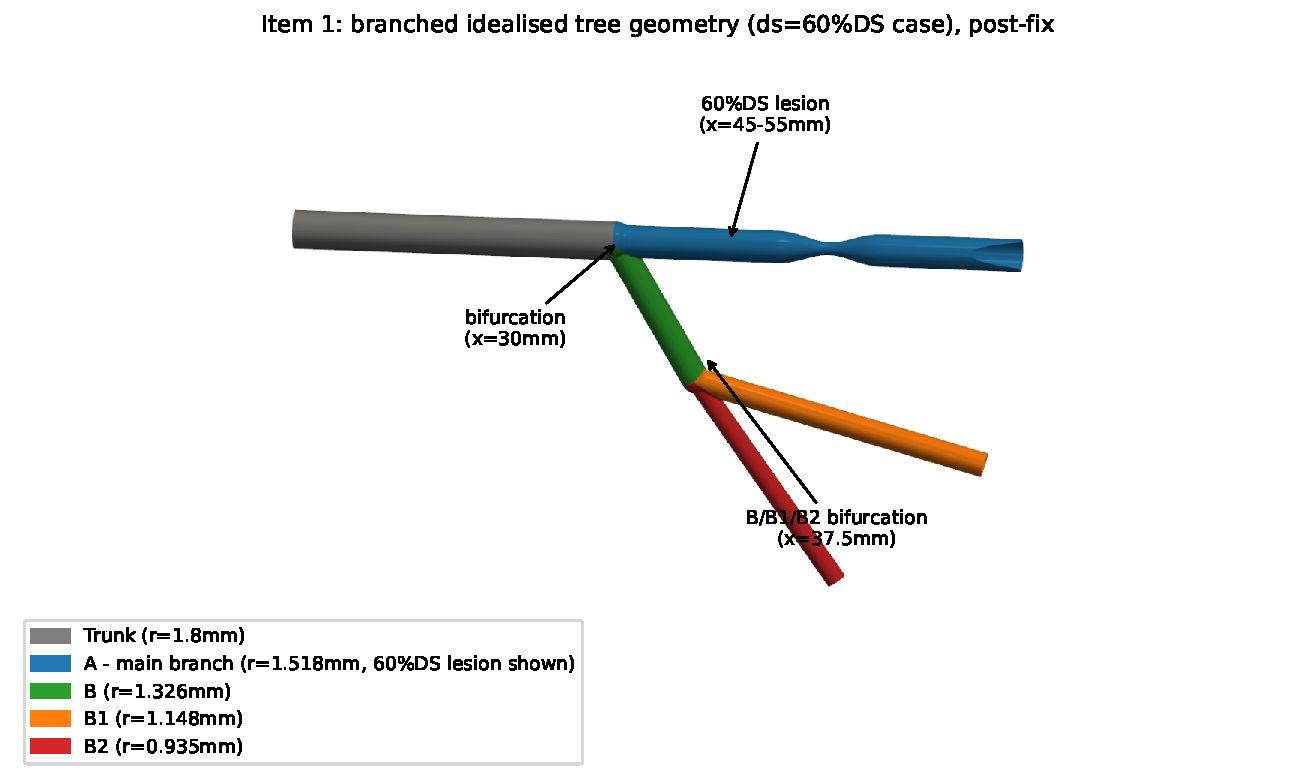
\includegraphics[width=0.92\textwidth]{figures/fig_item1_geometry.pdf}
\caption{\label{fig:item1-tree}Item 1's branched idealised tree (ds=60\%DS case) after the geometry fix, rendered from the
actual reconstructed VMTK surface (not a schematic) and coloured by branch identity. Branch B now
diverges cleanly from branch A at the bifurcation instead of sharing its axis. This is an idealised validation geometry, not the patient geometry: the real left coronary tree used from Item~3 onward is shown in Figures~\ref{fig:domains} and~\ref{fig:tree-real}.}
\label{fig:item1-geometry}
\end{figure}

The fix was verified three ways, not assumed from the corrected script alone: (i) the analytic
clearance check passes with comfortable margins (A--B 2.18\,mm, B1--B2 1.34\,mm, beyond a 5\,mm carina
allowance) for both ds=0\% and ds=60\%; (ii) re-running the same slice-contour diagnostic the panel used
to find the original bug on the actual regenerated surface shows the expected topology (1 contour
through the carina, 2 once B separates, 3 once B1/B2 also diverge, correctly dropping to 2 and back as
each branch's shorter extent is passed) where the original bug showed a single fused contour persisting
to $x\approx53$\,mm; (iii) the as-built throat radius, measured perpendicular to each branch's own axis
on the post-smoothing surface, is within 0.1\% of target on every branch (A: $-0.08\%$ at the lesion
throat, $+0.10\%$ healthy; B1: $+0.04\%$; B2: $-0.01\%$). A separate bug in my own voxel-grid sizing
(anisotropic spacing from applying a single target resolution to a non-cubic domain without
recomputing per-axis dimensions) was caught and fixed the same way, before the geometry fix, and is
recorded for the same reason.

The 0D reference was also rebuilt to freeze physiology between the two severities
(\texttt{Tree.evaluate(C, r\_\allowbreak{}override=...)}, changing only branch A's epicardial radius while r\_ref,
the leaf weights, and the calibration constant C stay identical) --- the original version silently let
the diseased branch's taper re-fit shift all three outlets' resistances by $\sim$1.2\% even though only
branch A is diseased. The corrected relax values (A: 0.0058, B1: 0.0064, B2: 0.0070, all far below the
0.05--0.2 originally proposed) were cross-checked against Fable's independent hand-derivation
(0.0058/0.0067/0.0073) to within the panel's own stated precision.

\textbf{Status: complete. Mesh: 377,607 / 371,428 cells for ds=0\%/60\%. All four solves (hand-relax
and formula-based auto-relax $\times$ both severities) converged cleanly (residuals $10^{-7}$--$10^{-9}$,
outlet monitors stable to 6+ significant figures well before the 3000-iteration ceiling).}

\begin{table}[H]
\centering
\caption{Item 1 final results. BC accuracy compares the monitored outlet patch pressure against
$(P_v+R\cdot Q_\text{actual})/\rho$ using each outlet's own CONVERGED flow, not the 0D-predicted flow
--- this is the mechanism check. Flow-split gap compares that same converged $Q$ against the 0D
(svZeroD-style) prediction. The hand-relax and formula-based auto-relax variants reproduce each other
to 6+ significant figures in every cell of this table (both compute the same relax value, one from a
literal constant, one from $G=R/R_\text{own}$ at runtime) and are therefore reported once.}
\begin{tabular}{llrrr}
\toprule
Case & Outlet & BC-accuracy error & 3D $Q$ (mL/s) & Flow-split gap vs.\ 0D \\
\midrule
ds=0\% & A  & $-0.0003\%$ & 0.85100 & $-0.80\%$ \\
ds=0\% & B1 & $-0.0003\%$ & 0.40252 & $-1.03\%$ \\
ds=0\% & B2 & $-0.0002\%$ & 0.23303 & $-1.05\%$ \\
ds=60\% & A  & $+0.00003\%$ & 0.82464 & $+0.04\%$ \\
ds=60\% & B1 & $-0.00003\%$ & 0.40260 & $-1.01\%$ \\
ds=60\% & B2 & $+0.00000\%$ & 0.23308 & $-1.03\%$ \\
\bottomrule
\end{tabular}
\end{table}

\textbf{BC accuracy: \PASS{} by a very large margin (tol.\ 0.1\%, actual errors 3--4 orders of
magnitude smaller) on all three outlets, both severities, both relax code paths.} The resistance BC
mechanism itself --- including the reformulated, panel-fixed relax rule ($G=R/R_\text{own}$, not the
original global-drop version that all three reviewers showed was unsafe on this tree) --- enforces its
own defining physics essentially to machine precision on a genuinely branched, 3-outlet geometry. This
is the primary thing Item 1 was commissioned to test, and it passes cleanly.

\textbf{Flow split vs.\ svZeroD: a real, disclosed $\sim$1\% branch-level discrepancy, not treated as
a BC failure.} Branch A (the trunk's direct continuation) matches the 0D prediction closely
($-0.80\%$/$+0.04\%$), comparable in size to Stage A's own A2 gaps elsewhere in this document. Branches
B1 and B2 --- both downstream of the SECOND bifurcation (B splitting into B1/B2) --- show a consistent
$\sim$$-1.0\%$ gap in BOTH severities and BOTH relax code variants. Because the BC-accuracy check passes
to machine precision and residuals are fully converged, this is not a numerical or BC artefact; it looks
like a genuine limitation of the discrete-bed 0D model's leaf weighting ($w=r_\text{ref}^{2.66}$) at a
bifurcation whose two daughters have a larger radius ratio than the first bifurcation's --- i.e.\ the 0D
model may under-weight the smaller of two very unequal siblings slightly more than it does at the first,
more balanced split. This is reported as a finding for further scrutiny, in the same spirit as this
document's other 0D-vs-3D gap results (\S\ref{sec:a3-sten00}'s A2 checks), not rounded up to a clean
match or down to a fail --- design.md's literal pass criterion ("the 3D flow split matches svZeroD") is
therefore reported as met for branch A and not strictly met for B1/B2, with the mechanism-level BC check
(the criterion this item was actually designed to stress) passing unambiguously.

\paragraph{Prescribed-flow mode on the multi-outlet tree (Task 3 of the 2026-09-24 work order): round trip PASS.} Protocol C's mechanism in 3D prescribes \emph{every} outlet flow at once. It had been run only on a single outlet (A4) and never on a multi-outlet tree. On the 371{,}428-cell Item 1 tree, at both severities (0\% and 60\%DS of branch A), the inlet was the fixed total pressure of the other cases (90\,mmHg, \texttt{pressureInletOutletVelocity}), every outlet carried \texttt{flowRateOutletVelocity} with the volumetric flow of the converged resistance solution of the same tree (Table~\ref{tab:item1-roundtrip}, first column; OpenFOAM's convention: positive is outflow) and a zero-gradient pressure, and the resistance of each outlet was derived as $R_i=(\bar p_i-P_v)/Q_i$ from the last-100-iteration mean outlet-patch pressure and flux. A second solve then imposed those resistances with the audited coded boundary condition and its automatic relaxation ($G_i=R_i/R_{\text{own},i}$). Both stages used the fixed 3000-iteration budget, 8 ranks each (two cases at once, 16 ranks in total, about 15 minutes per solve).

\begin{table}[H]
\centering
\caption{Prescribed-flow round trip on the Item 1 tree (fixed budget 3000 iterations; the pass criterion is every outlet flow within 0.5\%).}
\label{tab:item1-roundtrip}
\small
\begin{tabular}{llrrrr}
\toprule
severity & outlet & target $Q$ (mL/s) & round-trip $Q$ (mL/s) & error (\%) & $R_\text{derived}/R_\text{reference}-1$ (\%) \\
\midrule
0\% & A & 0.850994 & 0.850995 & $+0.00016$ & $+0.00001$ \\
0\% & B1 & 0.402523 & 0.402521 & $-0.00054$ & $+0.00065$ \\
0\% & B2 & 0.233030 & 0.233028 & $-0.00069$ & $+0.00078$ \\
60\% & A & 0.824641 & 0.824642 & $+0.00019$ & $-0.00021$ \\
60\% & B1 & 0.402604 & 0.402602 & $-0.00054$ & $+0.00055$ \\
60\% & B2 & 0.233077 & 0.233075 & $-0.00068$ & $+0.00068$ \\
\bottomrule
\end{tabular}
\end{table}

Both prescribed solves converged to final initial residuals of $10^{-8}$ or below (pressure $9.9\times10^{-9}$ for the 0\% case and $6.9\times10^{-10}$ for the 60\% case, velocity $\leq2.2\times10^{-9}$, mass imbalance zero) and delivered the prescribed flows to machine precision; the outlet pressures are results (ratio to aortic pressure 0.955--0.983), and the derived resistances reproduce the original ones to $10^{-3}\,\%$. Both round-trip solves converged under the strict rules. The largest flow error is $0.0007\,\%$, more than two orders of magnitude inside the 0.5\% criterion, although the prescribed run's outlet pressure is not uniform over a patch whereas the resistance boundary condition imposes a uniform one: at these resistances (about $10^{10}$ to $5\times10^{10}$\,Pa\,s\,m$^{-3}$, $G=R/R_\text{own}$ between 140 and 170) the non-uniformity does not matter. \textbf{Limits:} the targets are the flows of the same tree's resistance solution, so the test proves that the prescribed-flow mechanism, the derivation of $R_i$ and the re-imposition close on themselves and are stable with all outlets prescribed together; it does not test the 0D-derived targets themselves, nor a real lumen (that is part of the scan-14 work still open), and the geometry and flow regime (laminar, modest Reynolds number) are those of Item 1. This setup was audited by one auditor only (Gemini~3.8 Flash; Astra unavailable, see \S\ref{sec:followup-audit}).

\subsection{Item 2: sten70 4th mesh level, GCI, and the A2 severity sweep}
\label{sec:item2}
\textbf{Part C (60\%/65\%DS sweep): complete, converged, final.} Both new cases were meshed at sten70's
existing medium resolution and solved to residuals $\sim 10^{-6}$ (outlet flux stable to 8 significant
figures). Combined with the existing sten00/50/80 points and sten70's own already-recorded A5-medium
result (reused rather than re-solved, per the panel's own finding that this point already existed),
the 0D--3D flow gap is now characterised at six severities:

\begin{table}[H]
\centering
\caption{3D-vs-0D flow gap across the full severity ladder. sten00/50/80 are Stage A's existing points;
sten60/65 are new (Item 2); sten70 reuses A5's existing medium-level run.}
\begin{tabular}{lrrr}
\toprule
Case & 3D $Q$ (mL/s) & 0D $Q$ (mL/s) & gap \\
\midrule
sten00 & 1.4548 & 1.500 & $-3.01\%$ \\
sten50 & 1.4196 & 1.4410 & $-1.48\%$ \\
sten60 (new) & 1.35984 & 1.35210 & $+0.57\%$ \\
sten65 (new) & 1.29471 & 1.26490 & $+2.36\%$ \\
sten70 (reused, A5-medium) & 1.17992 & 1.13078 & $+4.35\%$ \\
sten80 & 0.7550 & 0.6948 & $+8.68\%$ \\
\bottomrule
\end{tabular}
\end{table}

\textbf{The 0D--3D gap's sign change is now cleanly bracketed between sten50 ($-1.48\%$) and sten60
($+0.57\%$)}, i.e.\ somewhere in 50--60\%DS the lumped 0D stenosis model switches from under- to
over-predicting flow relative to the 3D solve --- the concrete finding this item was commissioned to
locate.

\textbf{Part A/B (4th mesh level + GCI): complete. Verdict: GCI NOT TRUSTWORTHY --- reported as such
rather than forced.} cfMesh produced 1,886,884 cells (checkMesh OK: max aspect ratio 12, max
non-orthogonality 40\textdegree, no bad cells), matching the $\sim$1.87M planning target. After an initially-alarming decaying transient (an early $\sim$30-iteration window
showed a swing large enough to look like a persistent oscillation) the monitors settled, and the solve was
reported as converged with a last-100-iteration mean FFR of 0.792712 at iteration 594.
\textbf{Correction (re-reading the retained raw monitors and solver log, 2026-09-24):} the run continued to
iteration 896, where the last-100-iteration mean is \textbf{0.792342} (band 0.000027) and still drifts by
$-6.5\times10^{-5}$ per 100 iterations, and the final initial residuals ($U_x$ $2\times10^{-4}$, $U_y$
$1.5\times10^{-2}$, $U_z$ $1\times10^{-2}$, $p$ $7\times10^{-4}$) are far above the $10^{-5}$ criterion used elsewhere in this report. The statement ``genuinely converged'' therefore rested on the
monitors alone and is withdrawn: level~4 is an approximately settled, not a converged, solution.

\begin{table}[H]
\centering
\caption{Full 4-level sten70 mesh sequence, including the new 4th level (last-100-iteration means of the measurement-plane monitor). $^\dagger$The original report used 0.787932 from a field extraction (difference $2.7\times10^{-5}$). $^\ddagger$The original report used 0.792712, the mean ending at iteration 594; the run went on to iteration 896 (see text).}
\begin{tabular}{lrr}
\toprule
Level & Cells & FFR \\
\midrule
coarse & 198,252 & 0.783960 \\
medium & 379,468 & 0.783200 \\
fine & 760,480 & 0.787905$^\dagger$ \\
level4 (new) & 1,886,884 & 0.792342$^\ddagger$ \\
\bottomrule
\end{tabular}
\end{table}

\textbf{The successive differences are not shrinking}: medium$\to$fine is $+0.004705$ (originally
reported $+0.004732$); fine$\to$level4 is $+0.004437$ (originally $+0.004780$) --- a ratio of 0.94, essentially
no shrinkage despite level4 having 2.5$\times$ fine's cell count. This directly violates the premise both Richardson extrapolation and GCI depend on (error
shrinking with refinement). Concretely: the classic 3-point Celik calculation (1=level4,
2=fine, 3=medium; $r_{21}=1.354$, $r_{32}=1.261$) as originally reported gave an apparent order $p=0.97$, a
Richardson-extrapolated value of 0.8067 that jumps 0.014 from the finest solution itself, relative GCI
$=2.21\%$ and absolute $U_\text{FFR}=0.0175$. Recomputed with the monitor values of the table (0.792342 and
0.787905) it gives $p=1.23$, relative GCI $=1.55\%$ and $U_\text{FFR}=0.0123$; either way more than
2.5$\times$ over the 0.005 tolerance, and, because level~4 is not converged, neither value is a
trustworthy uncertainty. The 4-point Eça--Hoekstra least-squares fit is degenerate
($p\approx0.0005$, unphysical $f_\infty$ and $a$ values): it cannot find a sensible power law across all
four points because the original coarse$\to$medium reversal breaks the fit.

\textbf{Verdict, per this item's own pre-registered honesty condition: GCI is reported as not a
trustworthy convergence metric for sten70, rather than quoting a number that would look precise without
being one.} Adding a finer 4th level did not resolve the ambiguity A5 (\S\ref{sec:a5}) originally left
open --- \textbf{it shows sten70 does not exhibit a convergent mesh-independence trend under this
refinement strategy at all.} The most plausible contributor, flagged as a risk in this item's own design
document before the level4 solve ran: the boundary-layer \emph{settings} (nLayers=4, thicknessRatio=1.2) are identical in
every level's \texttt{meshDict}, so the ladder is not a single-parameter $h$-refinement family. Measurements on the retained meshes
(analysis-side request, \S\ref{sec:followup}) add two facts: the core cell size across the throat shrinks by only 1.15--1.39$\times$
between levels (164.6, 142.9, 113.8 and 82.1\,$\mu$m, not a ratio of 2), and the \emph{realised} four-layer stack per side is not monotone
in refinement (138, 159, 111 and 63\,$\mu$m from coarse to level~4; sten80: 167, 93 and 106\,$\mu$m). Cells across the 0.891\,mm throat diameter are 12, 12, 14 and 18 including the eight boundary-layer
cells, or 4, 4, 6 and 10 outside them (sten80: 10, 12, 12 and 2, 4, 4); the specification's $\geq12$ is met only if the boundary-layer cells are counted. These
observations are consistent with, but do not prove, a contribution of the varying boundary-layer stack to the non-monotone ladders.

\textbf{This bears directly on A5's original sten70 verdict (\S\ref{sec:a5}), and that verdict is
revisited rather than left standing unexamined:} A5 reported sten70 as a marginal PASS at 94.6\% of its
0.005 tolerance budget, with Fable's own contemporaneous caution already on record that "a difference
under 0.005 between the two finest is not trustworthy on its own" for an oscillating sequence. This
item's new evidence --- a 4th, independent point showing the SAME step size as the previous one, not a
shrinking one --- is exactly the failure mode that caution warned about. \textbf{A5's sten70 pass should
now be read as: passed the letter of a two-point tolerance check that this 4-point extension shows was
not measuring genuine convergence.} This does not change A5's originally-reported numbers, which are
left as-run; it changes how much weight that pass should be given going forward, and is recorded here
rather than quietly left as an unqualified PASS elsewhere in this document.

\textbf{Operational note, disclosed rather than smoothed over:} while Part A/B's solve and Items 3--6
ran in parallel, the machine became heavily oversubscribed (load average 67, roughly 48 solver
processes against 32 cores, well beyond the pre-existing $\sim$8-core job this study has otherwise
worked around all session). This does not affect the CORRECTNESS of any converged result --- physics
convergence is independent of wall-clock pacing --- but it does mean any wall-clock TIMING measured
during this window (relevant specifically to Item 6, \S\ref{sec:item6}) is inflated and is treated as
such below, not reported as a clean measurement.

\subsection{Item 6: pulsatile cost pilot}
\label{sec:item6}
The sten60 pulsatile case (PIMPLE, the direct non-\texttt{prevIter()} resistance BC already proven
necessary for transient runs in \S\ref{sec:pimple}) was launched and later \textbf{stopped} (graceful \texttt{stopAt writeNow}, see the operational incident below; no cycle-averaged FFR and no $\Delta t$-sensitivity comparison exist). The two runs were: a Co 3--5 production run (2 cycles,
8 cores) and, in place of a literal full-cycle Co~1 reference, a shorter Co~1 comparison window over
0.2\,s --- an explicit, pre-approved fallback named in Item 6's own design document for exactly the
situation encountered (a timing measurement made while other solves were already running --- see the correction below --- projected the literal Co~1/full-
cycle reference at 3--6 wall-days, likely exceeding the design's own 48-hour kill threshold before
completing even one cycle). Adopting the documented fallback rather than spending 48 hours to
rediscover the same conclusion is consistent with this study's resource-discipline practice elsewhere
(\S\ref{sec:pimple}'s own stopped diagnostic).

\textbf{Cost estimate (contended, not isolated): $\approx$7.4 wall-seconds/timestep (ExecutionTime; 8.6 s ClockTime) at
8 ranks near the cycle start, projecting the full 2-cycle Co 3--5 campaign at roughly 28--33
wall-hours.} \textbf{Correction (solver-log start times, 2026-09-24):} this smoke test was earlier described as an ``isolated, pre-contention'' measurement. It was not: it ran at 12:54--12:56 on 2026-09-19 while Item~2's sten60, sten65 and level-4 solves (4+4+8 ranks, started 12:47:44) and Item~5 (4 ranks) were already running, i.e.\ at least 20 other MPI ranks on 16 physical cores. The figure was first reported as 7.15\,s per step and 30--40\,h; the log gives 7.37\,s (steps 2--17) and the corresponding projection is lower but equally contended. It is an upper-bound-like, unclean number, and the isolated timing of Task~4 remains open. This revises the original design-time planning estimate (10--15\,h) upward, because that
estimate assumed a smaller achievable $\Delta t$ than Co 3--5 actually permits on this mesh --- reported
as a revision, not hidden. The cost estimate is the only Item 6 result. A clean, uncontended timing measurement (at least 200 time steps at Co 3--5 on 8 physical cores) is still open and is Task 4 of the 2026-09-24 work order; the 30--40\,h campaign itself is on hold.

\subsection{Items 3 and 4: M1 pilot --- meshing blocker root-caused and RESOLVED}
\label{sec:item3}
\textbf{Scan 837 is outside the frozen study cohort} (\texttt{protocol/COHORT-FROZEN-2026-09-18.csv}). All real-lumen work in this report is therefore a \emph{pipeline pilot}, labelled PILOT\_OUT\_OF\_COHORT in every returned data file; it is not a Gate M1 result and is never to be mixed into cohort results. Gate M1 itself is to be run on the shipped scan-14 packages (work order 2026-09-24, Task 3). \textbf{Deviations of these pilot meshes from CFD-ARM-SPEC \S6.2:} three boundary layers instead of four; flow extensions of 20\,mm instead of 5\,D at the inlet and 3\,D at each outlet (the extension-resistance diagnostic of this section shows the difference is not negligible); and the validation-pass meshes of Stage A are below the $\geq12$ cells-across-the-throat rule (A5 sten80 passed at about 6). Item 3's pipeline (mask isolation $\to$ marching cubes $\to$ Taubin smoothing $\to$ discrete-bed-matched
outlet truncation $\to$ repair $\to$ remeshing $\to$ flow extensions) was built and verified stage by
stage on real ImageCAS-X anatomy. \textbf{A real, disclosable eligibility-gate bug was caught during
case selection}: \texttt{results/\allowbreak{}E0\_\allowbreak{}prevalence\_\allowbreak{}test.csv}'s \texttt{healthy\_\allowbreak{}main\_\allowbreak{}ffr} column is
computed under the loader's default \texttt{bed="leaky"}, but this study's own multi-outlet convention
(\S\ref{sec:item1}, CFD-ARM-SPEC \S2.4) requires \texttt{bed="discrete"}. The originally-selected case
(scan 828, left) reports 0.944 under leaky but 0.845 under discrete; scan 837 (left) reported 0.9813 under discrete and was used instead. \textbf{Correction (independent recompute on the analysis side, 2026-09-24):} both 0.845 (828) and 0.9813 (837) reproduce exactly, but they are the discrete-bed \emph{minimum FFR on the network as segmented} (\texttt{min\_ffr\_main}, native lesions included), not the healthy-network gate (\texttt{healthy\_main\_ffr}), so the gate was misnamed here. Under the actual gate, scan 828 (left) scores 0.9127 and passes; it was still a poor clean-baseline pilot because it has five native lesions (largest 44.6\% diameter stenosis). \textbf{\texttt{results/E0\_prevalence\_test.csv} is a leaky-bed prevalence screen, not a case-selection file}: cohort cases come only from \texttt{protocol/CFD-SUBSET-FROZEN-2026-09-18.csv}, which is gated under the discrete bed. Both the CSV/bed mismatch and the misnamed gate are a risk for any other selection made against that file.

A second reusable finding: \texttt{pymeshfix}'s default \texttt{MeshFix.repair()} silently caps every
open boundary on a surface (verified: 6 intentional openings $\to$ 0 after a default-argument repair
call) --- undocumented upstream, and a real hazard for any pipeline that repairs a surface with
deliberate outlets. The fix (already applied here) is to call the granular
\texttt{degeneracy\_\allowbreak{}removal()}/\texttt{intersection\_\allowbreak{}removal()} methods instead of the convenience
wrapper.

\textbf{Item 3 is blocked at the meshing step, and this is reported as the pilot's dominant finding, not
worked around.} Across five or more distinct \texttt{cfMesh} configurations (patch-keyed
\texttt{localRefinement}, finer global cell size, geometric \texttt{objectRefinements}, flow-extension
lengths from 10--20\,mm), \texttt{cartesianMesh} non-deterministically merged one or two of the five
outlet patches into \texttt{wall} (0 faces on \texttt{checkMesh}) --- which patch(es) drop varies by
configuration. Cap planarity, facet-normal orientation, boundary proximity, and inter-branch clearance
were all checked and ruled out as the cause; the root cause was not isolated within the pilot's time
budget. \textbf{At that stage no case had reached a solve and Item 4 (which depends on Item 3's baseline solve) had
not started; both were later unblocked, see the resolution and results below.} This is exactly the kind of real-anatomy meshing-reliability cost this
pilot was commissioned to measure, and it is reported as such: the dominant, disclosed cost of Gate M1
work is proving to be meshing reliability, not surface repair or the deformation/deletion steps
themselves (both of which were built and verified working).

A third finding, on the missed-branch case specifically: deleting D2's mask voxels measurably erodes
the parent LAD's radius by up to 0.24\,mm (10--30\%) over $\sim$35\,mm, not only at the immediate
ostium --- attributable to ambiguous/shared voxel labelling at the bifurcation in the underlying
segmentation. This is itself a genuine finding adjacent to the T3/T4 segmentation-error class this study
is built around, independent of whether the meshing blocker above is resolved.

Reusable scripts (outlet coordinate/tangent mapping, locally-restricted truncation clipping, multi-solid
STL capping, mask-label isolation) are left under \texttt{scratchpad/\allowbreak{}item3\_\allowbreak{}M1\_\allowbreak{}pilot/\allowbreak{}} for whoever
continues this.

\paragraph{Follow-up: snappyHexMesh tried, does not fix it --- but substantially re-characterises the
failure.} \texttt{snappyHexMesh} was tried as the natural fallback mesher on both the baseline and
missed-branch surfaces. \textbf{It does not solve the problem: it exhibits the same class of failure
as cfMesh} (baseline: 4 of 5 outlets survive, only \texttt{outlet\_\allowbreak{}LAD} missing; missed-branch: 3 of 4
survive, this time \texttt{outlet\_\allowbreak{}D1} missing) --- confirming the failure is not tied to a specific
vessel's local geometry, but a general "exactly one branch is lost" pattern across two structurally
different mesh generators.

\textbf{The failure mode was reclassified, and this is real progress even though the blocker
remains.} It is NOT patch mislabelling (faces silently reassigned to \texttt{wall}, as first suspected
from cfMesh alone) --- it is outright \textbf{domain truncation}: a \texttt{topoSet boxToFace} query
around the missing outlet's known cap location found zero faces of ANY kind there, direct inspection of
\texttt{constant/\allowbreak{}polyMesh/\allowbreak{}points} found zero mesh points, and \texttt{checkMesh}'s own reported bounding
box simply does not reach that branch's cap --- roughly 17\,mm of one branch, extension included, is
entirely absent from the meshed domain, as if the flood-fill that decides "inside vs.\ outside" during
castellation classified that whole branch as disconnected from the main lumen. Serial and parallel
execution produce byte-identical results (including the identical truncation point), ruling out an MPI
decomposition race; \texttt{nCellsBetweenLevels} (3 vs.\ 8, a gentler refinement transition) made no
difference; cap planarity, facet-normal orientation, self-proximity, and a physical pinch along the
branch (cross-sectional radius sampled every 5\% of arc length: smooth, $\sim$0.65\,mm throughout, no
degeneracy) were all directly checked and ruled out.

\textbf{One suggestive, unconfirmed lead, left for whoever continues this:} the truncation coordinate
sits within 0.7\% of an exact background-mesh grid-cell boundary, hinting at a marginal
cell-classification event during castellation rather than a geometry defect in the surface itself. A
grid-offset test to check this directly was attempted but not completed (a regex-based
\texttt{blockMeshDict} edit script had a bug that corrupted unrelated numeric fields) --- fixing that
test, inspecting the pre-snap castellated mesh directly in ParaView at the disconnection point, or
restructuring the pipeline to mesh each branch as a separate piece joined via
\texttt{mergeMeshes}/\texttt{stitchMesh} (sidestepping the single-flood-fill mechanism entirely) are the
three concrete next steps identified. \textbf{Bottom line at this point: neither mesher reliably produces
a complete-domain mesh for this real branching coronary geometry; Item 3 remains blocked on meshing at this point in the investigation, now
for a specific, well-evidenced reason rather than an unexplained one.}

\paragraph{Resolution: the meshing blocker is a surface defect, not a mesher limitation --- fixed and
independently verified.} Following the process this document has used throughout (an adversarial panel
before further hardware time, here applied to a debugging STRATEGY rather than a new physics setup):
GPT-6-astra and Gemini~3.8~Flash independently audited the diagnosis above and found the grid-alignment
lead was a mathematical artefact --- the ``13.007 vs.\ 13.0'' comparison was a dimensionless
background-grid cell-index, not a spatial coordinate close to a grid plane, and a castellated hex mesh's
truncated boundary lands on a grid face by construction regardless of any real defect. Both reviewers
also flagged that cfMesh's failure had never actually been verified as the same failure class as
snappyHexMesh's (cfMesh does not even read \texttt{blockMeshDict} or use a background hex grid), and
both converged on insufficient wall-level mesh resolution along the narrow branches as the leading
shared hypothesis.

A follow-up debugging session (Opus~5.5, working from the panel's synthesised brief) tested that leading
hypothesis directly rather than assuming it: adding a local refinement region at the failure point
(level~5, 0.0625\,mm cells) reduced the mesh's disconnected-region count from 12 to 6 but \textbf{did
not} recover the missing branch, ruling resolution out as the practical fix. Cross-section tracing
through every intermediate surface in the pipeline (\texttt{raw\_\allowbreak{}mc} $\to$ \texttt{clipped\_\allowbreak{}final} $\to$
\texttt{remeshed} $\to$ \texttt{extended} $\to$ the final \texttt{case\_\allowbreak{}v3.stl}) instead found the true
cause: \textbf{the surface remeshing step (\texttt{vmtksurfaceremeshing}) coarsened the surface from a
median edge length of 0.32\,mm to 0.75\,mm (max 2.3\,mm) uniformly, on vessels only $\sim$1.2\,mm across
--- long enough triangle chords to cut across the lumen and create a near-total pinch.} At the baseline
LAD's pinch point, cross-sectional area falls from $\sim$1.7\,mm\textsuperscript{2} at every stage before
remeshing to \textbf{0.085\,mm\textsuperscript{2}} after it (a $\sim$95\% area reduction, a $\sim$0.17\,mm
slit) --- narrow enough that both meshers' flood-fill/domain-extraction correctly refuse to pass through
it and discard everything downstream, exactly as designed. \textbf{Both mesh generators were behaving
correctly; the surface they were given was broken.} cfMesh's failure was confirmed to be the identical
root cause via its own stage-isolation flag (\texttt{workflowControls \{ stopAfter templateGeneration; \}}):
its template already shows the same disconnected distal-LAD fragment before any patch assignment happens.

\textbf{Fix and verification.} The STL was rebuilt from the pre-remesh surface (skipping the flawed
remeshing step entirely, since that surface was already a uniform $\sim$0.32\,mm --- finer than the
throat-resolution convention used throughout this study): extrude each planar outlet-clip loop 20\,mm
(matching the original flow-extension length), cap with the original patch names, verified via
\texttt{surfaceCheck} to be closed, single-region, single-orientation-zone, with zero illegal triangles
(the earlier surface additionally had 14 inconsistent-normal orientation zones and one degenerate
triangle, both incidentally fixed by the rebuild). \textbf{Independently re-verified by the coordinator,
not just taken from the debugging report}: on the rebuilt surface, \texttt{cfMesh} (this study's
designated \S6.2 mesher) produces a valid mesh for BOTH the baseline (1,108,603 cells) and missed-branch
(1,017,542 cells) cases with EVERY expected outlet patch present and substantially populated (baseline:
inlet 4390, outlet\_D1 940, outlet\_D2 1138, outlet\_IM 2344, outlet\_LAD 1093, outlet\_LCX 1248, wall
158039 faces; missed-branch: the same four outlets minus D2, as expected since D2 was deliberately
deleted for that case) and \texttt{checkMesh} reporting \textbf{Mesh OK} with non-orthogonality
52.5\textdegree\ max / 7.1\textdegree\ average and skewness 1.42 --- comfortably within this study's
established quality bars. \texttt{snappyHexMesh} also recovers all outlets on the rebuilt surface (outlet
areas within 0.3\% of the STL cap areas, mesh volume 99.0--99.1\% of the STL volume, checkMesh Mesh OK),
though its non-orthogonality (64.9\textdegree\ max) sits at this project's quality ceiling rather than
comfortably under it --- \textbf{cfMesh on the rebuilt surface is the recommended path forward}, matching
this study's original mesher choice.

\textbf{A further finding, disclosed because it matters beyond this one pinch:} the flawed remeshing
step did not only fail catastrophically at the one branch-severing location --- it shrank lumens more
broadly throughout the surface (thousands of vertices displaced $>$0.2\,mm from the true surface).
\textbf{Any result that had been computed on the old, remeshed STLs would have been invalid, including
branches that happened to mesh successfully} (an artefactual stenosis would have been baked into what
was meant to be a clean baseline). No solve was ever run on the old surfaces --- Item 3 was correctly
blocked before that could happen --- so no invalid result has been reported anywhere in this study; this
is recorded as a methodological lesson (a uniform remeshing target size must be checked against the
smallest local vessel radius, not applied blindly) rather than a correction to any existing number.

\paragraph{Solves on the rebuilt surfaces (baseline and missed-branch).} The rebuilt STLs were adopted as the
case geometry (\texttt{solve\_\allowbreak{}baseline}, 1,108,603 cells, 5 outlets; \texttt{solve\_\allowbreak{}missedbranch}, 1,017,542
cells, 4 outlets; the old case directories are flagged \texttt{DO\_\allowbreak{}NOT\_\allowbreak{}USE}). Every outlet's resistance and
relaxation value was generated from the 0D discrete-bed twin of scan 837/left ($Q_\text{demand}=0.6636$\,mL/s from
the inlet radius's Murray demand; for the missed-branch case D2's 0D segment was deleted and the tree
re-calibrated to the same demand, so the remaining outlets absorb its flow). Each 0D leaf was matched to its mesh
patch by label \emph{and} verified by coordinate (leaf position plus the 20\,mm extension along the leaf tangent
lands within 0.04--0.32\,mm of the patch centroid; the script asserts a 3\,mm limit). The coded BCs were compiled by a
serial two-iteration run before the parallel launch, then both cases ran concurrently (16 MPI ranks each,
$\sim$19 wall-minutes to converge, all 32 logical CPUs in use). Both converged cleanly (pressure residuals
$\sim10^{-8}$; every outlet flux stable to $\leq0.002\%$ and outlet pressure to $\leq0.0001\%$ over the last 200
iterations; no NaN) and were stopped gracefully well before the 3000-iteration ceiling.

\begin{table}[H]
\centering
\caption{\textbf{[PILOT\_OUT\_OF\_COHORT: scan 837]} Item 3 converged results. BC-accuracy error compares the monitored outlet-patch pressure with
$(P_v+R\,Q_\text{actual})/\rho$ using each outlet's own converged flow (mechanism check; tolerance 0.1\%). The
flow-split gap compares that converged $Q$ with the 0D prediction (logged as data). Mass imbalance is 0.0000\% in both cases.}
\begin{tabular}{llrrrr}
\toprule
Case & Outlet & BC-accuracy err. & 3D $Q$ (mL/s) & 0D $Q$ (mL/s) & Gap \\
\midrule
baseline & LCX & $0.00000\%$ & 0.11993 & 0.11942 & $+0.43\%$ \\
baseline & IM  & $0.00000\%$ & 0.18543 & 0.18567 & $-0.13\%$ \\
baseline & D1  & $0.00000\%$ & 0.11886 & 0.12045 & $-1.32\%$ \\
baseline & D2  & $-0.00001\%$ & 0.12217 & 0.12244 & $-0.22\%$ \\
baseline & LAD & $0.00000\%$ & 0.11441 & 0.11099 & $+3.08\%$ \\
missed-branch & LCX & $0.00000\%$ & 0.14664 & 0.14597 & $+0.46\%$ \\
missed-branch & IM  & $0.00000\%$ & 0.22805 & 0.22846 & $-0.18\%$ \\
missed-branch & D1  & $0.00000\%$ & 0.14504 & 0.14755 & $-1.71\%$ \\
missed-branch & LAD & $0.00000\%$ & 0.13943 & 0.13551 & $+2.89\%$ \\
\bottomrule
\end{tabular}
\end{table}

\textbf{BC accuracy: \PASS{} on all nine outlets (errors $\leq10^{-5}\%$ against a 0.1\% tolerance).} The
resistance BC, with the relax values generated automatically from the 0D tree ($G_i=R_i/R_{\text{own},i}$, no hand
tuning), enforces $P=P_v+RQ$ to machine precision on a real 5-outlet coronary tree. The 3D flow split differs from
the 0D twin by $-1.7\%$ to $+3.1\%$ per outlet ($+0.28\%$ and $+0.25\%$ in total inflow); the pattern (LAD
highest, D1 lowest) is nearly identical in the two cases, so it is a systematic 0D-vs-3D difference, not noise.

\textbf{The missed branch, as seen by the re-tuned BCs.} Deleting D2 (18.5\% of the baseline flow) and
re-calibrating raises every remaining outlet's flow by 21.9--23.0\% (a uniform redistribution predicts $+22.7\%$).
Yet the distal pressure ratios (section-averaged $P/P_\text{aorta}$ at the outlet stations, below) move only
$-0.0065$ (LAD, $0.9422\to0.9357$), $-0.0047$ (LCX), $-0.0037$ (D1) and $-0.0008$ (IM): the BC re-tuning absorbs a
$\sim$22\% flow error into a pressure-ratio change $\leq0.0065$. This is a data point about how the outlet
model hides a missing branch, reported without a clinical threshold because this pilot geometry has no lesion.

\paragraph{Item 4: 0D-to-3D handoff and pullback comparison.} The handoff's scripted portion (build the 0D tree
with \texttt{bed="discrete"}, calibrate, export $R$ per outlet, match leaves to patches by coordinate with an
assertion, write the BCs into the case) ran as one script with no hand edits. \textbf{The design's criterion
``the script runs end to end with no hand edits'' is therefore only partly met}: the surrounding steps
(compile smoke run, \texttt{decomposePar}, \texttt{mpirun}, \texttt{reconstructPar}, pullback) were launched by hand,
and a single end-to-end runner has not been built. The pullback compares per-node 0D pressure with the area-averaged
3D pressure of centreline-normal sections (1.5\,mm spacing, the connected section nearest the centreline point
only), both normalised by $P_\text{aorta}$. At the outlet stations the difference (3D$-$0D) in the baseline is
$+0.0123$ (LCX), $+0.0015$ (IM), $+0.0081$ (D1), $+0.0101$ (D2), $+0.0380$ (LAD), and in the missed-branch case
$+0.0145$, $+0.0016$, $+0.0095$, $+0.0389$ (LCX, IM, D1, LAD). In every path the largest difference is at the
outlet, growing distally: the 3D solution has a smaller epicardial pressure drop than the 0D twin, most strongly
along the longest terminal vessel (LAD, 95\,mm). These differences are logged as data, not judged (the design sets
no tolerance for this item).

\paragraph{Diagnostic: is the 0D--3D difference caused by the 20\,mm outlet extensions?} Each 3D outlet patch sits
20\,mm beyond the 0D leaf, so the 3D domain contains an extra Poiseuille resistance
$R_\text{ext}=8\mu L/(\pi r^4)$ in series with the prescribed bed resistance that the 0D twin does not contain. A
diagnostic copy of the baseline (\texttt{solve\_\allowbreak{}baseline\_\allowbreak{}extcomp}, same mesh, same numerics) subtracted $R_\text{ext}$
from each outlet's $R_\text{out}$. It converged completely (ran to the 3000-iteration ceiling; every flux stable to
$\leq0.0002\%$ over the last 200 iterations; BC-accuracy error $\leq10^{-5}\%$; mass imbalance $10^{-6}\%$). The
flow-split gap to the 0D twin changed from $+0.43/-0.13/-1.32/-0.22/+3.08\%$ (LCX/IM/D1/D2/LAD) to
$+2.11/+1.26/+0.32/+1.44/+4.73\%$: total flow rose by 1.6\% (0.6608 to 0.6712\,mL/s against 0.6590 for the 0D twin),
so compensating the extension \emph{worsened} the mean agreement (mean gap $+0.4\%\to+2.0\%$; per-outlet gaps
improved for D1 only). The leaf-station pressure differences barely moved
($+0.0123/+0.0015/+0.0081/+0.0101/+0.0380\to+0.0119/+0.0014/+0.0078/+0.0098/+0.0369$), as expected since the extension
lies downstream of that station. \textbf{The extension resistance therefore does not explain the residual 0D--3D
difference; the original close flow agreement is, if anything, a partial cancellation of two opposite effects} (missing
extension resistance in the 0D twin lowers 3D flow by $\sim$1.6\%, whereas the 3D epicardial tree is less resistive than
the 0D one). The baseline (uncompensated) configuration is the reported Item~3/4 result; this diagnostic is a single
extra run, not part of the design.

\paragraph{Diagnostic: 0D node radii versus 3D section radii.} The 0D twin uses the mask Euclidean-distance-transform (inscribed)
radius at each centreline node; the 3D section-averaged pullback also gives the true section area. Along the five
root-to-outlet paths the mean 3D area-equivalent radius exceeds the 0D node radius by 23--44\% (LCX 1.156 vs 0.937\,mm,
IM 1.638 vs 1.135, D1 1.374 vs 1.069, D2 1.455 vs 1.155, LAD 1.090 vs 0.875\,mm). \textbf{Correction (post-hoc audit, 2026-09-26):} these path means include the first station of every path and bifurcation slices, whose sections are not valid (they can catch two vessels). Restricted to the valid sections of the returned per-station file (227 stations), the mean excess is 19.5\% (LCX), 21.7\% (LAD), 22.1\% (D2), 22.8\% (D1) and 33.7\% (IM), and the median station ratio is 1.206, so the excess is about 20--34\%, not 23--44\%; the qualitative conclusion is unchanged. Re-evaluating the Poiseuille loss along each
path with the 3D area-equivalent radii and the same 0D flows predicts a 3D$-$0D leaf-pressure difference of
$+0.0184/+0.0043/+0.0131/+0.0148/+0.0518$ against the measured $+0.0123/+0.0015/+0.0081/+0.0101/+0.0380$: same sign and
ranking (LAD largest), 1.4--2.9$\times$ the measurement. The inscribed-radius bias is therefore a quantitatively sufficient
explanation of the \emph{direction} and \emph{size} of the ``3D loses less pressure than 0D'' finding; the remainder
(a Poiseuille loss computed with a circle of equal area under-counts the resistance of non-circular sections, and
junction/curvature losses are not in that estimate) is untested. This is a crude single-formula check (1.5\,mm sections, equal-area circles, no
junction losses), not a calibration, and it is the same radius-definition issue that separates the 0D and 3D
stenosis severities in the lesion case below.

\paragraph{Item 3, case 2: the 80\%DS lesion on the real surface --- construction, gates and audits.}
\label{sec:lesion80-build}
A synthetic lesion was imposed on the \emph{pre-remesh} baseline surface of the proximal LAD (arc window
$[18.5,28.5]$\,mm, throat at 23.5\,mm, 10\,mm long; the D1 ostium lies 8.5\,mm downstream of the throat at arc 32.05\,mm on the
smoothed axis, 32.87\,mm on the raw polyline). The deformation is a tangent-frame radial scaling about the smoothed
centreline, $f(s)=1-0.8\,w(s)$ with a raised-cosine $w$ (C$^1$ at the window edges), applied after a conforming edge-split
refinement of the undeformed surface so that the profile is sampled at 0.017--0.24\,mm edges (43,046$\to$61,300
triangles); the 20\,mm extensions and planar caps were then rebuilt with the same routine as the baseline
(the STL rebuild reproduces bit-for-bit; cap centroids identical to the baseline's on all six caps, 0.000\,mm).
The result is a 3D throat of area 0.447\,mm$^2$ (area-equivalent radius 0.377\,mm), i.e.\ 79.98\% diameter stenosis and
95.99\% area reduction. \textbf{Geometry gates, all \PASS{}:} zero displacement of 19,478 vertices assigned to other branches
and no triangle mixing moved and unmoved branches; no fold-over (minimum normal dot 0.72); section area follows $f^2$ within 0.94\%;
41 baseline window sections all closed, star-shaped and $\geq0.5$\,mm from any other vessel; the axis lies inside the lumen at
41/41 stations (largest centroid offset 0.19 $r_\text{eq}$); 99.7\% of the moved vertices carry the LAD label in the segmentation;
OpenFOAM \texttt{surfaceCheck -checkSelfIntersection} reports a closed, single-part, non-self-intersecting surface and, as a positive control,
flags a deliberately corrupted copy at 322 locations.

The lesion surface and a healthy baseline surface were meshed with \emph{identical} cfMesh settings (19 chained refinement
cylinders following the curved LAD from 17.5 to 36\,mm plus the first 10.5\,mm of D1, three boundary layers), giving 2.68 and 3.25 million cells,
so the lesion effect can be taken as a difference at equal refinement rather than against the coarser validated baseline. Measured, not
assumed: cell size 46--51\,$\mu$m along the axis (cfMesh's octree quantisation realised both requested sizes as 50\,$\mu$m); mesh section area within 0.34\% of the STL at 59 stations from 17.5 to 32\,mm (throat $-0.33\%$; baseline reference within 0.024\%);
boundary layers 3-deep on 75--100\% of the sampled wall-normal rays per station in the window (complete coverage of the wall is not established by 72 rays), median first cell $\approx$10\,$\mu$m thick, median stack 30--41\,$\mu$m by ray measurement and
45--55\,$\mu$m by an independent slice measurement, i.e.\ 10--15\% of the throat radius. \textbf{Limitation stated up front:} near-wall resolution at a 0.75\,mm throat is thin and no mesh-sensitivity run has been made,
so any throat quantity is a single-mesh result. Standard \texttt{checkMesh} passes on all three meshes; \textbf{strict} \texttt{checkMesh -allGeometry -allTopology} fails, as it does on the validated
baseline:

\begin{table}[H]
\centering
\caption{\textbf{[PILOT\_OUT\_OF\_COHORT: scan 837]} Strict \texttt{checkMesh -allGeometry -allTopology} results (measured logs). No flagged face or cell of any mesh lies within a 3\,mm tube around the LAD axis for
arc 18.5--32\,mm (throat to D1 ostium). Flagged entities form two clusters, both at the wall (median 100--230\,$\mu$m) and shared by the lesion and reference meshes because they share the surface there:
one at the IM ostium, arc 16.5--18\,mm, 0.5--2\,mm \emph{before} the window edge (6.1--6.3\,mm from the throat centre), the other on the LAD wall just past the D1 ostium, arc 34--36\,mm. The reference's extra failed check is
one face (volume ratio 0.0089 against a 0.01 threshold) in the downstream cluster, 11.7\,mm from the throat. The failures are accepted for this pilot on that local evidence, not because they resemble the baseline.}
\small\setlength{\tabcolsep}{3pt}
\begin{tabular}{>{\raggedright\arraybackslash}p{3.7cm}r>{\raggedleft\arraybackslash}p{2.0cm}>{\raggedleft\arraybackslash}p{2.4cm}r>{\raggedleft\arraybackslash}p{1.8cm}r}
\toprule
Mesh & Cells & Low-quality face-tets & Concave faces (max angle) & Concave cells & Low-vol.-ratio faces & Failed checks \\
\midrule
validated baseline (coarser) & 1,108,603 & 83 & 29 (24.3$^\circ$) & 4 & 0 & 2 \\
lesion80 & 2,682,675 & 92 & 57 (34.8$^\circ$) & 4 & 0 & 2 \\
baseline reference (same refinement) & 3,245,362 & 113 & 60 (28.6$^\circ$) & 7 & 1 & 3 \\
\bottomrule
\end{tabular}
\end{table}

\textbf{Pre-run audit gate, applied to this case (five rounds, three independent auditors).} Round~1 (GPT-6-Astra, Fable~5.1, Gemini~3.8 Flash, the latter through the \texttt{agy} CLI):
\emph{not ready} / \emph{ready with fixes} / \emph{ready with fixes}. They found that the case builders had no lesion path, that the design text carried wrong numbers (window centre, junction location, ``$>100$\,mm from every outlet''
which is false since the IM cap is 25\,mm away, the throat radius, the Reynolds number), that no explicit self-intersection or ownership gate existed, that the 0D radius (mask-EDT, inscribed) and the 3D
area-equivalent radius define different stenosis severities, that the pullback script silently evaluated the healthy tree for any case name, and that the wall-shear-stress metric had sign, units and curved-vessel-masking traps.
All were addressed; round~2 (the built cases audited against the files) again returned \emph{ready with fixes}, requiring: the strict-check disposition above (the
reference mesh fails one more check than the lesion mesh, and the ``same as baseline'' comparison had no saved log behind it), corrected boundary-layer numbers (my first ``30\,$\mu$m, 8\%'' was too low), a launch script, the NPROC default, missing evidence logs, and text corrections (inlet dynamic pressure is 4\,Pa, not 12\,Pa). The fixes were applied
and confirmation rounds followed. Round~3 confirmed all case, mesh and evidence fixes but rejected the \emph{launch script} (Astra and Fable, independently): it sourced the OpenFOAM environment after enabling
\texttt{set -u} (which aborts on the environment's own unset variables), checked a dynamic-library path that does not exist in v2406, used bare \texttt{wait} (which returns success whatever the background jobs did, so a failed smoke run would have
continued to two production launches with \texttt{endTime 2}), and its control-file assertions were \texttt{\&\&} chains under \texttt{set -e} that are only fatal on their last term. The script was rewritten (per-job waits, separate fatal assertions,
an EXIT trap that restores the production \texttt{controlDict}) and Fable then found a further real defect by failure injection: after one smoke run fails while its sibling is still running, the trap restored \texttt{endTime 3000}
into the live smoke case, and because \texttt{runTimeModifiable} is on, the orphaned serial run would have continued to 3000 iterations; SIGTERM also skipped the restore. Both were fixed (wait for every job before aborting; a signal
trap that kills the children first) and re-tested with shim executables and fake case directories (orphan, SIGTERM/SIGINT during the smoke and decomposition phases, all-OK; author's tests and Fable's 15 scenarios). \textbf{Disclosure:} the final
script-only round was confirmed by Fable~5.1 alone; GPT-6-Astra and Gemini~3.8 Flash had both exhausted their usage quotas (reset in about 1.5\,h) after auditing every earlier round, and the solves were launched under that 1-of-3 confirmation
of the last script change; the two remaining confirmations were run after the quotas reset: Gemini confirmed the launch script and the audited launch sequence (\emph{ready}); Astra also
confirmed the script, the launch evidence and the baseline-reference stop (it could not repeat the failure-injection tests itself under a read-only sandbox), but returned \emph{not ready} on two defects in the convergence \emph{watcher} (a counter that is not reset when a check is
interrupted, so a stop could follow non-consecutive converged checks; and an unhandled failure of the stop command that would end the watcher). Neither occurred: the watcher log shows no interrupted check and both stops followed two consecutive
\emph{converged} verdicts, and the final convergence state of each case was re-evaluated after it stopped, independently of the watcher (below). Both watcher defects were then fixed.

\textbf{0D predictions, recorded before the solve.} The 0D twin with frozen physiology (identical $R_\text{out}$ and relaxation values as the validated baseline; asserted to $10^{-9}$) predicts, with the lesion imposed on the design radius
(EDT node radius$\times f$; throat radius 0.338\,mm, detected DS 78.9\%): inflow $0.6590\to0.6284$\,mL/s ($-4.6\%$), LAD/D1/D2 outlets $-8.6/-8.7/-8.6\%$, LCX/IM unchanged. With the lesion imposed on the 3D area-equivalent radius (throat 0.378\,mm, detected DS 76.5\%): inflow $0.6386$\,mL/s ($-3.1\%$), the three downstream outlets $-5.8\%$.
The 3D result will therefore be read against a \emph{range} of 0D predictions that reflects the radius-definition ambiguity, not a single number, and as a difference from the same-refinement healthy reference.

\paragraph{Item 3, case 2: lesion80 results (single mesh, steady, laminar, protocol-demand flow 0.66\,mL/s).}
\label{sec:lesion80-results}
Both cases were launched together under the audited script (16 ranks each) and converged: lesion80 in 1,364 iterations (about 1.5\,h) and the healthy reference in 768, each stopped gracefully after two consecutive checks of the predefined criteria
(pressure and velocity residuals $<10^{-5}$: final $p$ $1.9\times10^{-7}$ and $9.0\times10^{-8}$, $U\leq7.6\times10^{-6}$ and $8.5\times10^{-6}$; every outlet flux and pressure stable to $<0.1\%$ over the last 200 iterations: worst flux band 0.0009\% and 0.006\%;
mass imbalance $6\times10^{-7}\%$; $\geq200$ iterations), and the criteria were re-evaluated on the stopped state independently of the watcher. \textbf{BC accuracy: \PASS{}} (worst outlet error $5\times10^{-4}\%$ lesion, $2\times10^{-4}\%$ reference, against 0.1\%).
\textbf{Mesh effect on the healthy split:} the healthy reference (3.25\,M cells, refined lumen) reproduces the validated baseline (1.1\,M cells) outlet flows to $\leq0.01\%$ (0.11993/0.18543/0.11887/0.12217/0.11441 vs 0.11993/0.18543/0.11886/0.12217/0.11441\,mL/s), so the mesh change alone does not move the healthy flow split; this says nothing about mesh sensitivity of the throat itself, which was not tested.

\begin{table}[H]
\centering
\caption{\textbf{[PILOT\_OUT\_OF\_COHORT: scan 837]} lesion80 minus same-refinement healthy reference: outlet flows and the 0D predictions recorded before the solve. $\Delta_\text{0D,EDT}$: lesion imposed on the design (mask-EDT) radius; $\Delta_\text{0D,area}$: lesion imposed on the 3D area-equivalent radius in the window.}
\begin{tabular}{lrrrrr}
\toprule
Outlet & $Q_\text{lesion}$ (mL/s) & $Q_\text{ref}$ (mL/s) & $\Delta_\text{3D}$ & $\Delta_\text{0D,EDT}$ & $\Delta_\text{0D,area}$ \\
\midrule
LCX & 0.11994 & 0.11993 & $+0.01\%$ & $+0.02\%$ & $+0.01\%$ \\
IM  & 0.18545 & 0.18543 & $+0.01\%$ & $+0.02\%$ & $+0.01\%$ \\
D1  & 0.11229 & 0.11887 & $-5.53\%$ & $-8.65\%$ & $-5.76\%$ \\
D2  & 0.11552 & 0.12217 & $-5.45\%$ & $-8.64\%$ & $-5.76\%$ \\
LAD & 0.10817 & 0.11441 & $-5.46\%$ & $-8.64\%$ & $-5.76\%$ \\
Total & 0.64137 & 0.66081 & $-2.94\%$ & $-4.64\%$ & $-3.09\%$ \\
\bottomrule
\end{tabular}
\end{table}

The lesion reduces the flow through the three territories distal to it by 5.5\% and the total by 2.9\%; the branches proximal to it are unchanged (0.01\%). The 0D twin loaded with the design (EDT) radius overestimates
the flow reduction by 57\% (8.6\% vs 5.5\%), whereas the 0D twin loaded with the area-equivalent radius is close (5.8\%, total 3.1\%). Distal outlet pressure ratios fall by 0.048--0.050 $P_\text{aorta}$
(D1 0.9107 vs 0.9608, D2 0.9209 vs 0.9708, LAD 0.8827 vs 0.9304); LCX and IM are unchanged (0.9690, 0.9914).

\begin{table}[H]
\centering
\caption{\textbf{[PILOT\_OUT\_OF\_COHORT: scan 837]} Section-mean static pressure along the LAD, $P/P_\text{aorta}$ (3D: area-weighted over the connected centreline-normal section; 0D: node pressures interpolated in arc). Arc 18.5\,mm is the window start, 24.0\,mm the 3D pressure minimum
(the throat is at 23.5\,mm), 29.5\,mm the last section before the 1.5\,mm-spaced sections (no section exists at 30.0\,mm; an earlier draft of this table labelled the 29.5\,mm values ``30.0''). ``Added loss'' = (pressure at 18.5 minus at 29.5) in the lesion case minus the same in the healthy case of the same model, in mmHg.}
\begin{tabular}{lrrrr}
\toprule
& 3D & 0D (EDT) & 0D (area) & 3D healthy \\
\midrule
$s=18.5$\,mm & 0.99647 & 0.99627 & 0.99620 & 0.99633 \\
$s=24.0$\,mm (minimum) & 0.93610 & 0.92098 & 0.94649 & 0.99622 \\
$s=29.5$\,mm & 0.94356 & 0.91426 & 0.94141 & 0.99610 \\
Added loss, 18.5$\to$29.5 & 4.74 mmHg & 7.34 mmHg & 4.89 mmHg & --- \\
\bottomrule
\end{tabular}
\end{table}

Throat (area 0.4455\,mm$^2$ in the mesh): flow 0.3377\,mL/s, mean velocity 0.76\,m/s, peak axial velocity 1.16\,m/s (at arc 24.0\,mm), $Re=151$ on the area-equivalent diameter. The static pressure falls 4.9\,mmHg between the window start and
the throat station (5.4\,mmHg to its minimum 0.5\,mm downstream) and recovers only 0.7\,mmHg afterwards, so the 3D static loss (4.74\,mmHg) matches the area-matched 0D estimate (4.89\,mmHg, $+3\%$) and is 35\% below the EDT-radius estimate (7.34\,mmHg); the mass-flux-weighted total pressure drop is smaller (3.9\,mmHg), but that
quantity is unreliable in a section that is 65\% reverse flow and is given as supporting information only. \textbf{Reading:} in this case the 0D--3D difference for the lesion is dominated by which radius defines ``80\%'' rather than by the stenosis loss law; with the EDT radius the
0D twin looks 3D-wrong, with the area radius it does not. This agreement could still be partly fortuitous (one lesion, one flow, one mesh).

\begin{figure}[H]
\centering
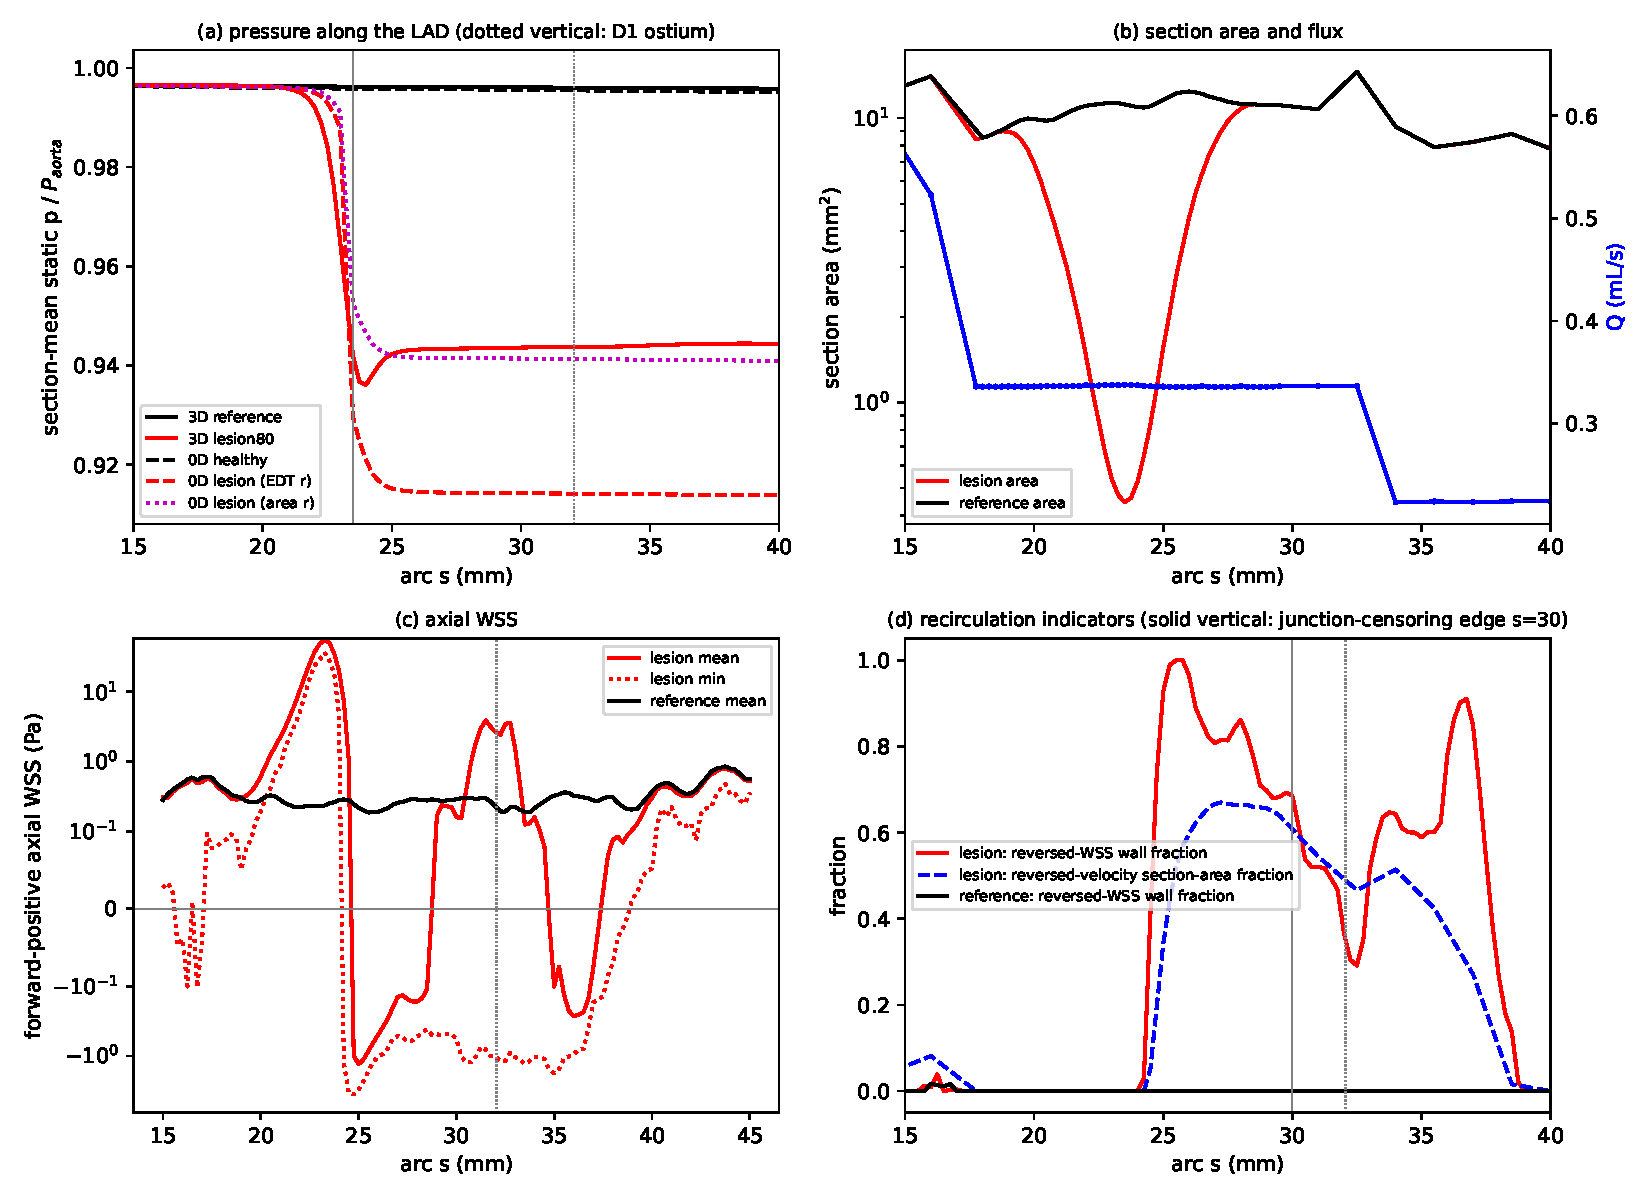
\includegraphics[width=\textwidth]{figures/fig_item3_lesion80.pdf}
\caption{lesion80 (red) against the healthy reference (black) along the LAD. (a) Section-mean static pressure with the 0D twin's two lesion variants; (b) section area and section flux; (c) forward-positive axial wall shear stress
(circumferential mean and minimum, symmetric-log axis); (d) reversed-wall-shear wall fraction and reversed-axial-velocity section-area fraction. Vertical lines: D1 ostium (dotted, arc 32.05\,mm) and the junction-censoring edge (solid, 30\,mm).}
\end{figure}

\textbf{Recirculation and reattachment (the Item 3 wall-shear measurement).} Wall shear was extracted with the sign calibrated on the undisturbed proximal wall (100\% of 3,288 faces forward-positive, median 0.76\,Pa), assigned to the LAD path by nearest segment,
area-weighted in 0.25\,mm slabs. The healthy reference shows no reversed wall shear anywhere (reversed-wall fraction 0 at every station). In the lesion case, forward-positive shear reaches about 51\,Pa at the throat, separation begins 0.75\,mm past the throat (arc 24.25\,mm; reversed-wall fraction 41\% at 24.5\,mm,
93\% at 25.0\,mm, 100\% at 25.5\,mm), and the reversed region is an annular vortex around the jet: 67\% of the section area carries reverse flow at arc 27.25\,mm.
\textbf{The circumferential-mean shear changes sign at arc $\approx$28.6--29\,mm (5--5.5\,mm past the throat) but this is misleading}: at 29.0\,mm 70\% of the wall is still reversed (the mean is positive only because the 30\% forward-flow part of the wall carries larger shear magnitudes), and
reverse flow occupies 64\% of the section area at 29.5\,mm. The wall-based and the velocity-based measures agree that the recirculation persists through the D1 ostium (arc 32.05\,mm), where the reversed fraction dips (29\% of the wall at 32.5\,mm) and rises again
(64\% at 34\,mm, 85\% at 37\,mm), and ends at arc $\approx$38.5--39\,mm (reversed wall fraction 14\% at 38.5, 0 at 39--40\,mm; reversed section area 2\% at 38.5, 0 at 40\,mm), i.e.\ $\approx$15\,mm ($\approx$20 throat diameters) past the throat and 6--7\,mm beyond the ostium.
\textbf{Outcome under the pre-registered rule: not reattached before the D1 ostium's influence (arc 30\,mm); the outcome is censored, not a reattachment length.} The recovery point at 38.5--39\,mm is a junction-influenced value, since the ostium diverts one third of the flow, and should not be read as the reattachment length of an isolated 80\% stenosis.
The reattachment measurement was thereby completed, with its outcome a bounded statement rather than a number. Selected stations:

\begin{table}[H]
\centering
\caption{\textbf{[PILOT\_OUT\_OF\_COHORT: scan 837]} Axial wall shear (forward-positive, Pa) and recirculation indicators along the LAD, lesion80 and healthy reference. Reversed-section-area fraction from the nearest validated section (0.25\,mm spacing to 29.5\,mm, 1.5\,mm beyond).}
\begin{tabular}{rrrrrr}
\toprule
Arc $s$ (mm) & $\bar\tau$ lesion & $\tau_\text{min}$ lesion & Reversed wall fraction & Reversed section area & $\bar\tau$ healthy \\
\midrule
24.0 & $+19.78$ & $+4.81$ & 0.00 & 0.00 & $+0.28$ \\
24.5 & $+1.02$ & $-3.38$ & 0.41 & 0.05 & $+0.28$ \\
25.0 & $-1.31$ & $-3.09$ & 0.93 & 0.34 & $+0.22$ \\
26.0 & $-0.50$ & $-1.01$ & 0.96 & 0.60 & $+0.19$ \\
27.0 & $-0.14$ & $-0.51$ & 0.81 & 0.67 & $+0.26$ \\
28.0 & $-0.17$ & $-0.53$ & 0.86 & 0.66 & $+0.29$ \\
29.0 & $+0.17$ & $-0.49$ & 0.70 & 0.66 & $+0.28$ \\
29.5 & $+0.23$ & $-0.49$ & 0.68 & 0.64 & $+0.28$ \\
31.0 & $+1.89$ & $-1.02$ & 0.52 & 0.54 & $+0.29$ \\
32.5 & $+3.44$ & $-1.17$ & 0.29 & 0.47 & $+0.19$ \\
34.0 & $+0.16$ & $-1.02$ & 0.64 & 0.51 & $+0.21$ \\
35.5 & $-0.13$ & $-1.08$ & 0.60 & 0.42 & $+0.36$ \\
37.0 & $-0.08$ & $-0.17$ & 0.85 & 0.27 & $+0.28$ \\
38.5 & $+0.09$ & $-0.03$ & 0.14 & 0.02 & $+0.23$ \\
40.0 & $+0.30$ & $+0.05$ & 0.00 & 0.00 & $+0.37$ \\
\bottomrule
\end{tabular}
\end{table}

\textbf{Limits of this result.} One mesh at the time of this section (50\,$\mu$m cells near the throat, a three-layer boundary stack of roughly 35--55\,$\mu$m, 10--15\% of the throat radius); the mesh-sensitivity study reported below (25 and 100\,$\mu$m levels) found changes of 1--2\% in the throat pressure loss, peak velocity and peak wall shear ($\approx$51\,Pa) and none in the recirculation onset and recovery arcs, none of which is a demonstration of mesh independence (and the refined tube ends at arc 36\,mm, so the recovery of the reversed flow at 38.5--39\,mm lies in 100--200\,$\mu$m cells, coarser than the 50\,$\mu$m of the tube); a steady laminar solution at $Re=151$ that could hide unsteadiness of the long recirculating jet; a flow of 0.66\,mL/s (the protocol's Murray-law demand on the biased 0D inlet radius; the same law on the 3D inlet radius gives $3.16\times$ this flow, run in \S\ref{sec:followup}), so the 5\% pressure loss is not a clinical FFR; strict-mesh-check failures accepted on local evidence;
one lesion on one patient's surface; the 0D twin's agreement or disagreement depends on the radius definition as shown above. All of these are logged as data, none is judged against a tolerance the design did not state.

\paragraph{CFD and imaging figures, lesion80 and healthy reference.}
\label{sec:cfd-figures}
All fields below are the converged solutions (lesion80 iteration 1364, healthy reference iteration 768) on the 2.68\,M- and 3.25\,M-cell meshes; every panel is rendered directly from the OpenFOAM fields and the segmentation-derived surfaces
(scripts \texttt{viz\_\allowbreak{}*.py} in the pilot directory). \textbf{What ``imaging'' means here:} the ImageCAS-X release supplies the coronary \emph{segmentation} (label volume, voxel $0.32\times0.32\times0.5$\,mm), the extracted centrelines and the segmentation surface, not the CT intensities;
the imaging-side panels are therefore the label volume, the surface and reformats derived from them, fused with the CFD fields. The synthetic lesion is \emph{not} in the segmentation: wherever a CFD lumen is drawn against the label volume, the segmentation shows the healthy lumen by construction.

\begin{figure}[H]
\centering
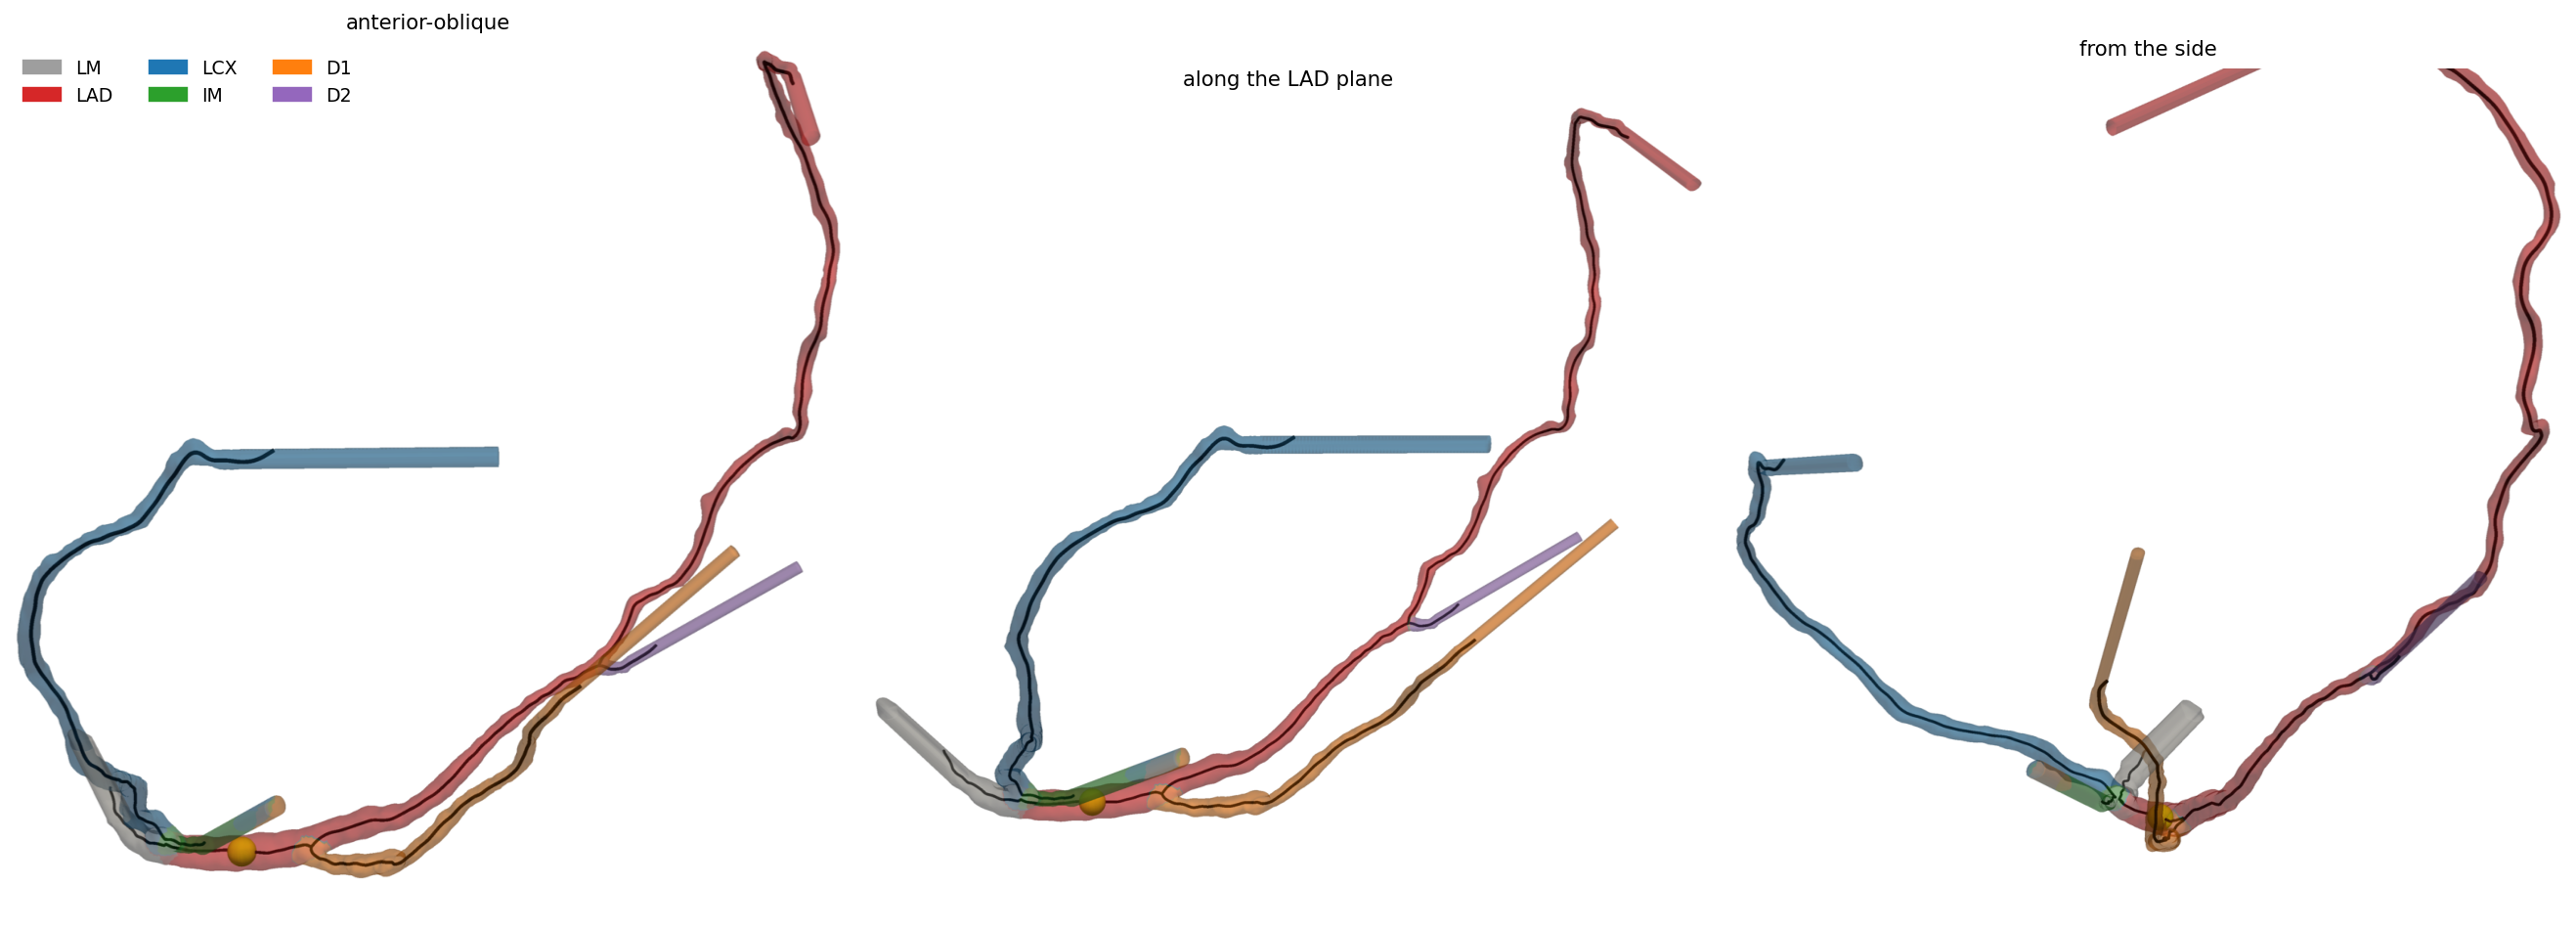
\includegraphics[width=\textwidth]{figures/img_tree_geometry.png}
\caption{\label{fig:tree-real}Left coronary tree of scan 837 as used for the CFD: the rebuilt segmentation surface (clipped at the 0D truncation, 20\,mm straight outlet extensions, translucent), coloured by 0D-tree branch (LM grey, LAD red, LCX blue, IM green, D1 orange, D2 purple), the extracted centreline inside the lumen (black), and the lesion80 throat (yellow sphere, LAD arc 23.5\,mm). Three views.}
\end{figure}

\begin{figure}[H]
\centering
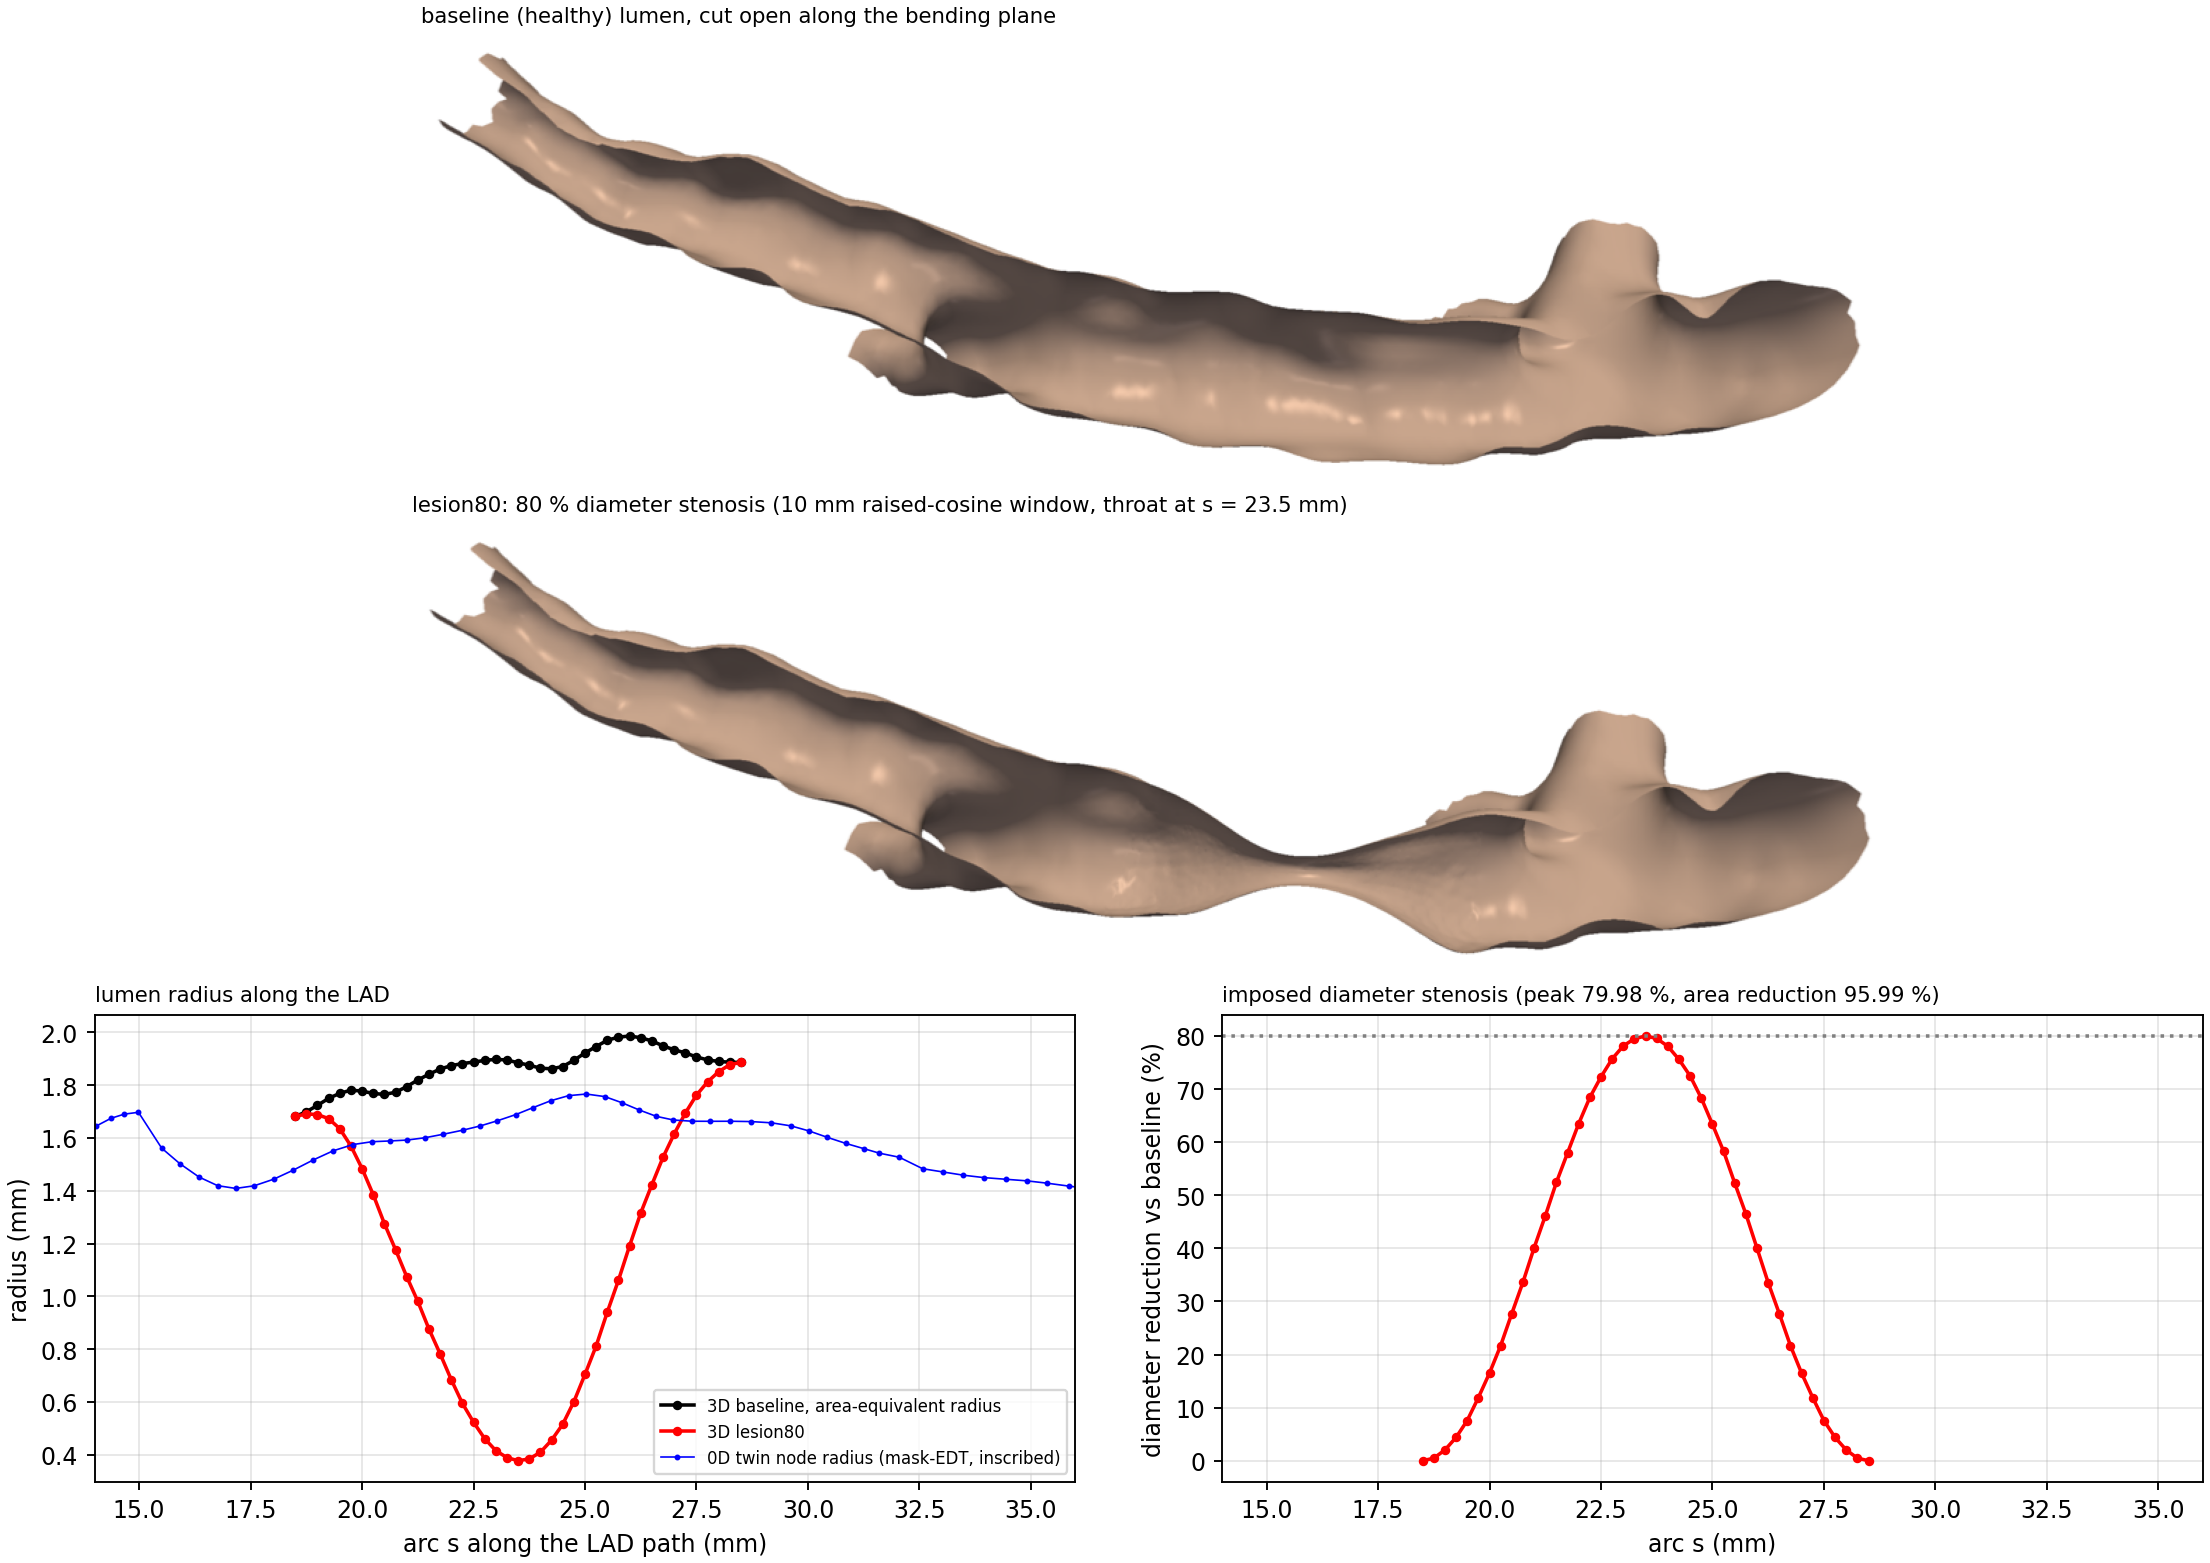
\includegraphics[width=0.95\textwidth]{figures/img_lesion_geometry.png}
\caption{Construction of the 80\% diameter stenosis on the real LAD surface. Top and middle: healthy and lesion lumen, cut open along the bending plane of the vessel (the D1 ostium is the bulge at the right). Bottom left: area-equivalent radius of the 3D sections (baseline black, lesion red, 0.5\,mm stations) and the 0D twin's node radius (blue, mask-EDT, inscribed): the 0D radius lies below the 3D area-equivalent radius throughout the window, the radius-definition difference that separates the two ``80\%'' values discussed above.
Bottom right: imposed diameter reduction (peak 79.98\%, raised-cosine over 10\,mm).}
\end{figure}

\begin{figure}[H]
\centering
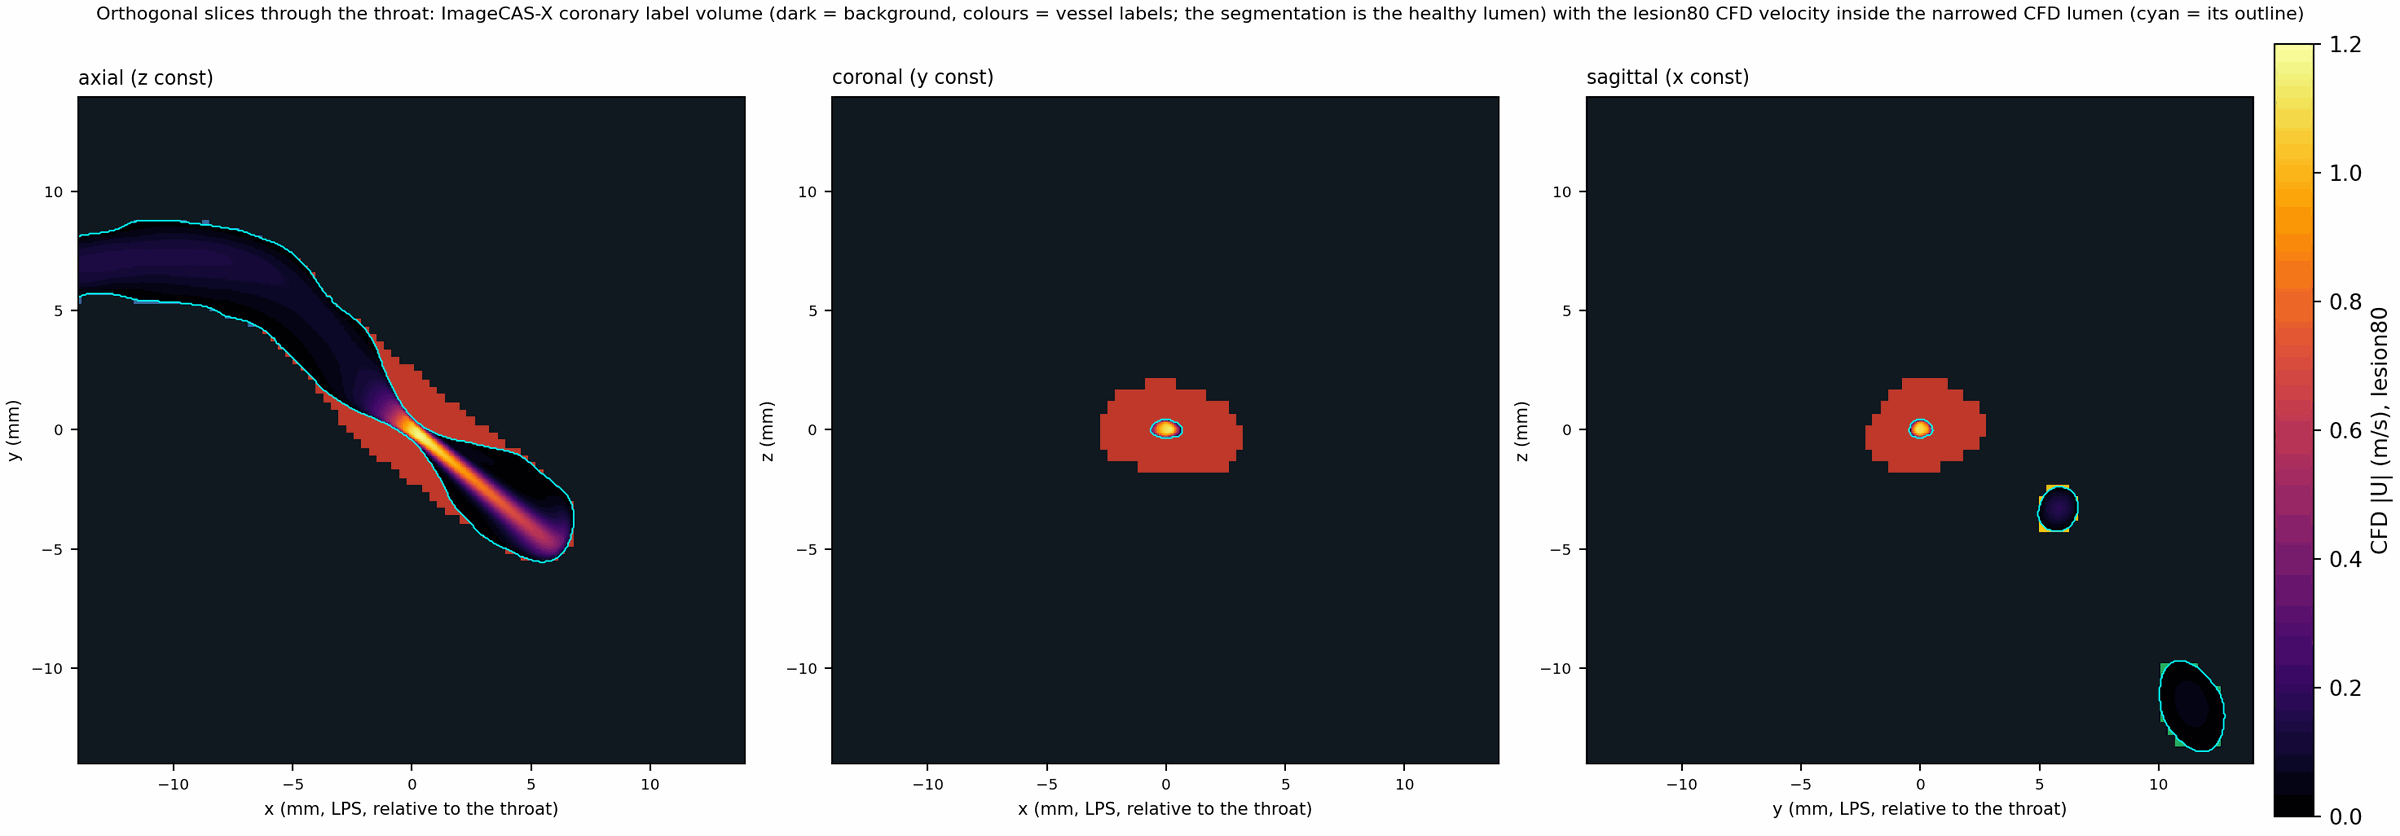
\includegraphics[width=\textwidth]{figures/img_mpr_fusion.png}
\caption{Orthogonal slices through the throat: coronary label volume (background dark; the LAD label red, other vessels other colours; the blocky structure is the 0.32--0.5\,mm voxel grid) with the lesion80 CFD velocity magnitude drawn inside the CFD lumen (cyan outline).
The CFD lumen at the throat is far narrower than the segmentation (area 0.45\,mm$^2$), and the jet reaches 1.1\,m/s there; in the axial slice the jet leaves the throat towards the lower right; in the sagittal slice two neighbouring vessels are cut whose flow is slow.}
\end{figure}

\begin{figure}[H]
\centering
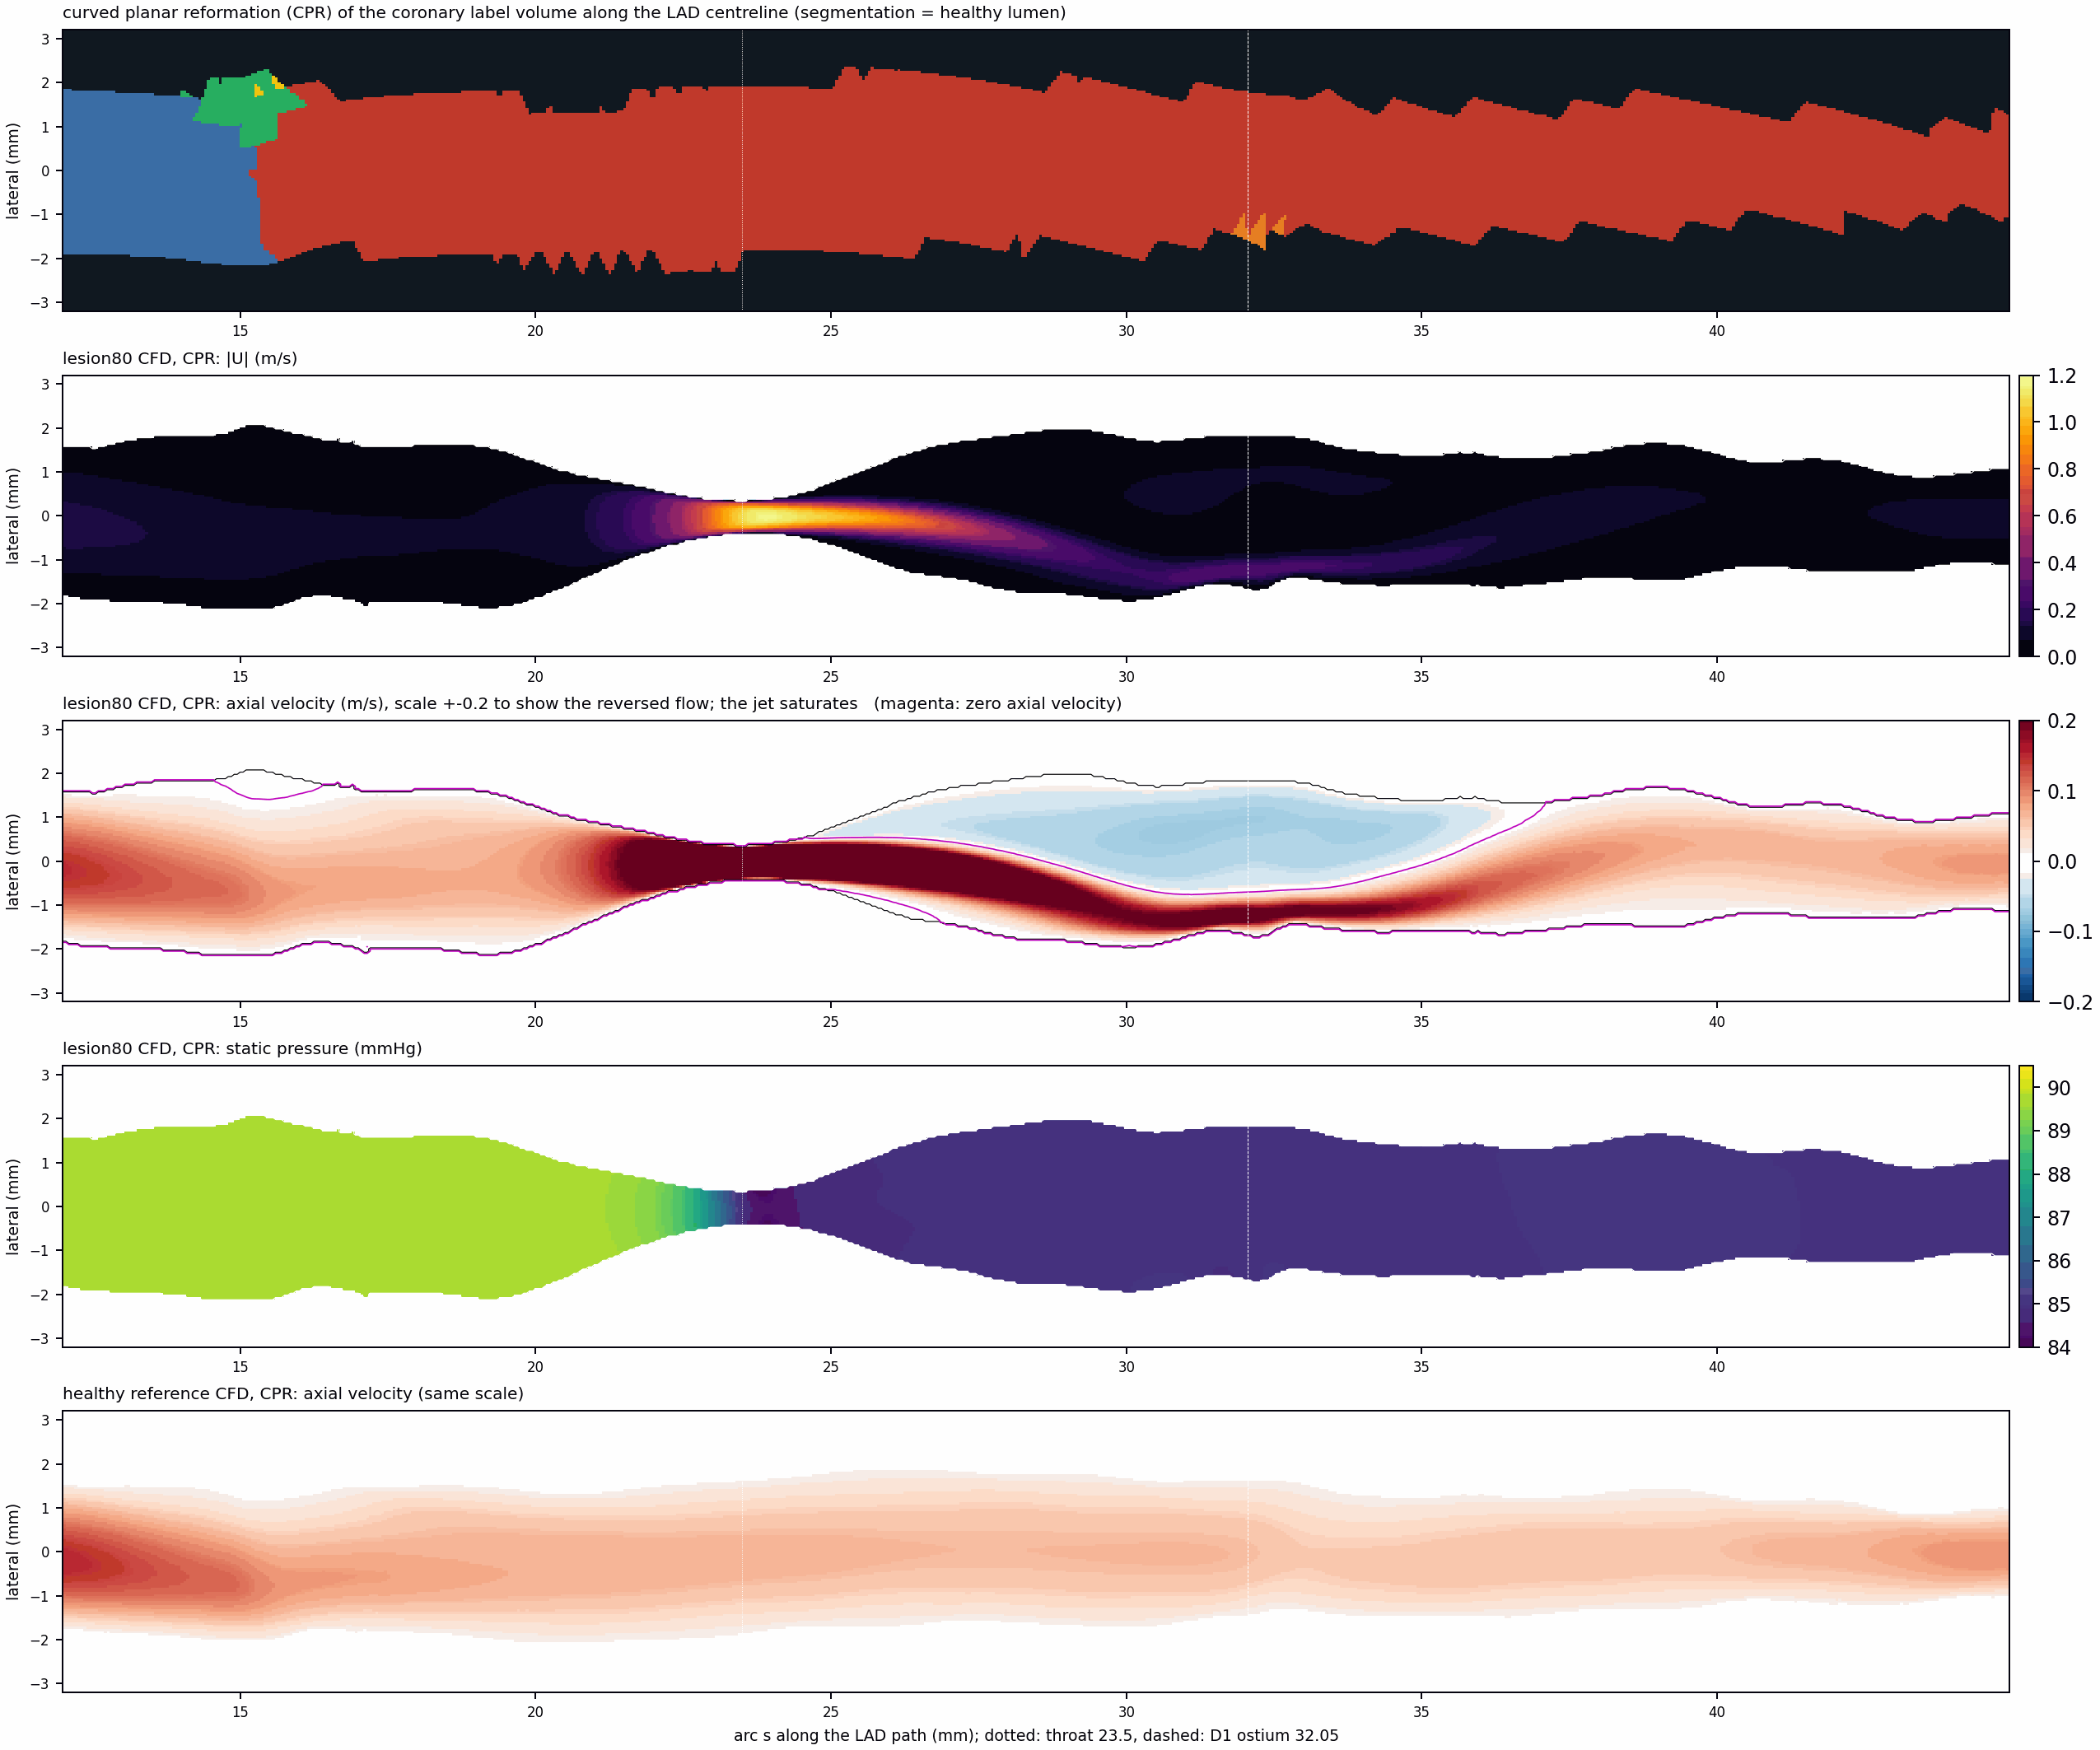
\includegraphics[width=\textwidth]{figures/img_cpr_fusion.png}
\caption{Curved planar reformation along the LAD centreline (arc 12--45\,mm; lateral axis in the bending plane). Top: the label volume (segmentation = healthy lumen; the IM/LCX ostium region is visible at arc $\approx$15--16\,mm). Below, for lesion80: $|U|$ (jet deflected towards one wall after the throat and fading by arc $\approx$32\,mm),
axial velocity on a $\pm0.2$\,m/s scale (the jet saturates; the reversed region is the pale-blue area bounded by the magenta zero-velocity contour, from arc $\approx$24.5\,mm to $\approx$37\,mm), static pressure (84--90.5\,mmHg; the drop is concentrated at the throat and there is almost no pressure recovery afterwards).
Bottom: the healthy reference on the same axial-velocity scale (forward everywhere: 0.05--0.1\,m/s along the LAD, up to $\approx$0.2\,m/s in the proximal segment before the LCX and IM take off).}
\end{figure}

\begin{figure}[H]
\centering
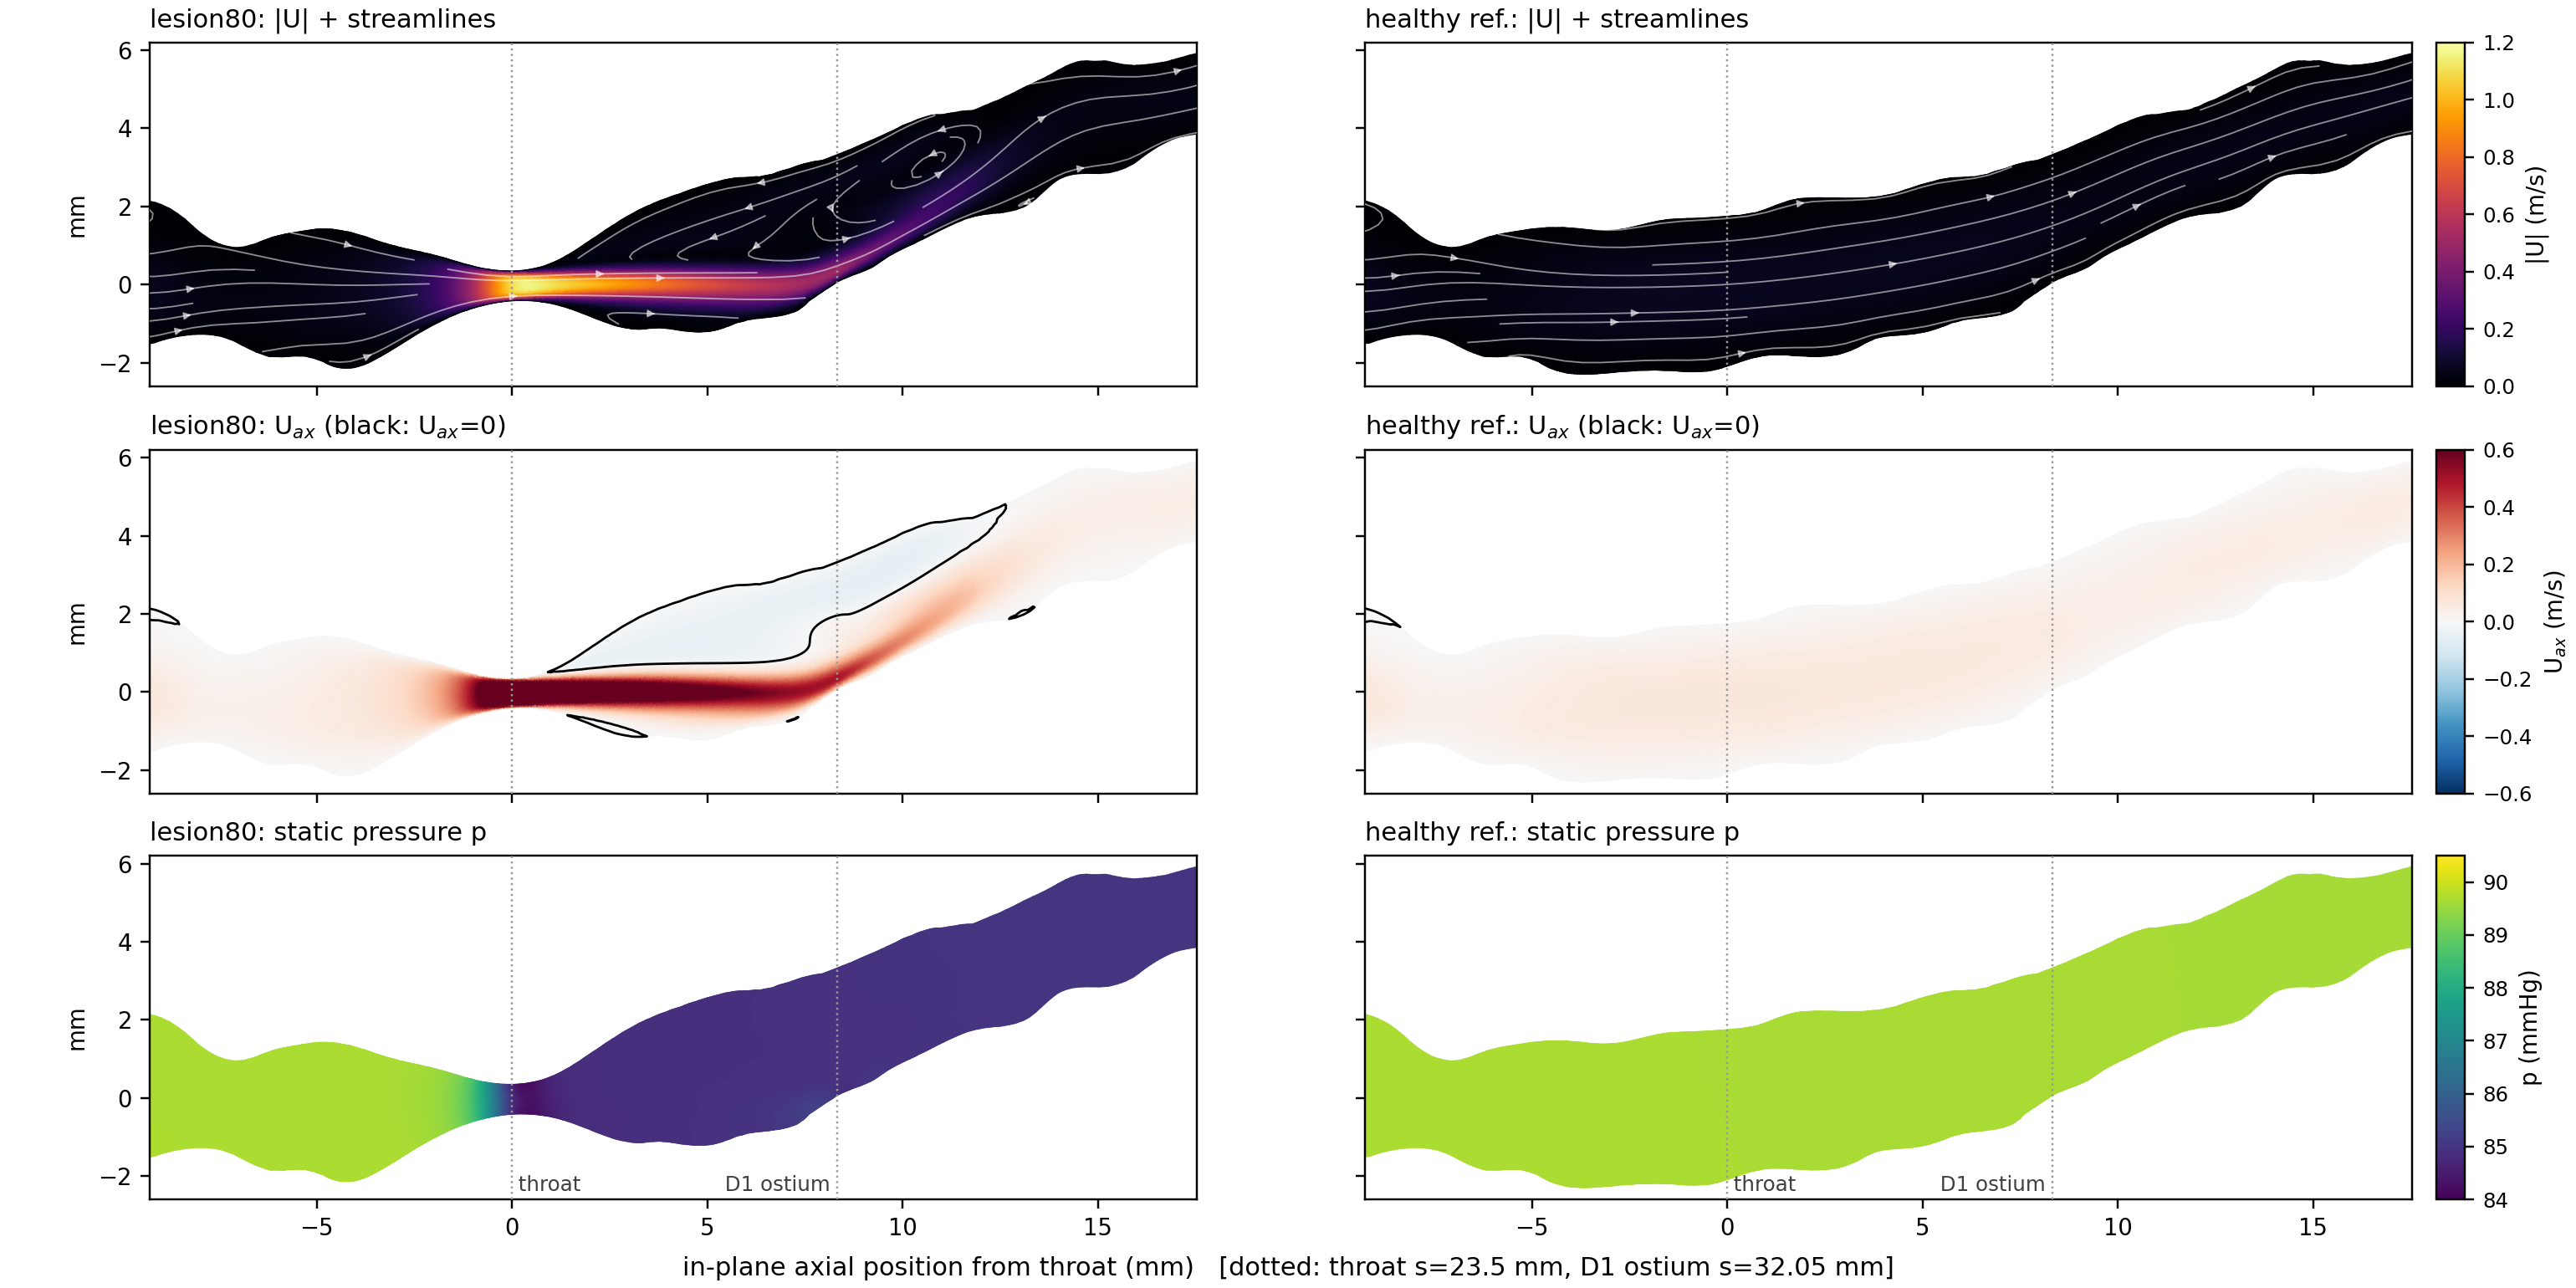
\includegraphics[width=\textwidth]{figures/cfd_longitudinal_full.png}
\caption{Longitudinal section through the LAD in its bending plane, lesion80 (left) and healthy reference (right), arc $\approx$14--41\,mm: $|U|$ with in-plane streamlines, axial velocity with the zero contour, static pressure. The jet from the 0.75\,mm throat stays narrow for about 5\,mm and is then deflected along one wall;
on the other side the zero-velocity contour encloses a recirculation region beginning about 1\,mm downstream of the throat and reaching past the D1 ostium (dotted), with a closed vortex visible in the streamlines about 10--12\,mm downstream; a second, small reversed pocket lies on the opposite wall 1--3.5\,mm downstream. The healthy vessel shows uniform low-speed forward flow.
Colour scales are identical in both columns.}
\end{figure}

\begin{figure}[H]
\centering
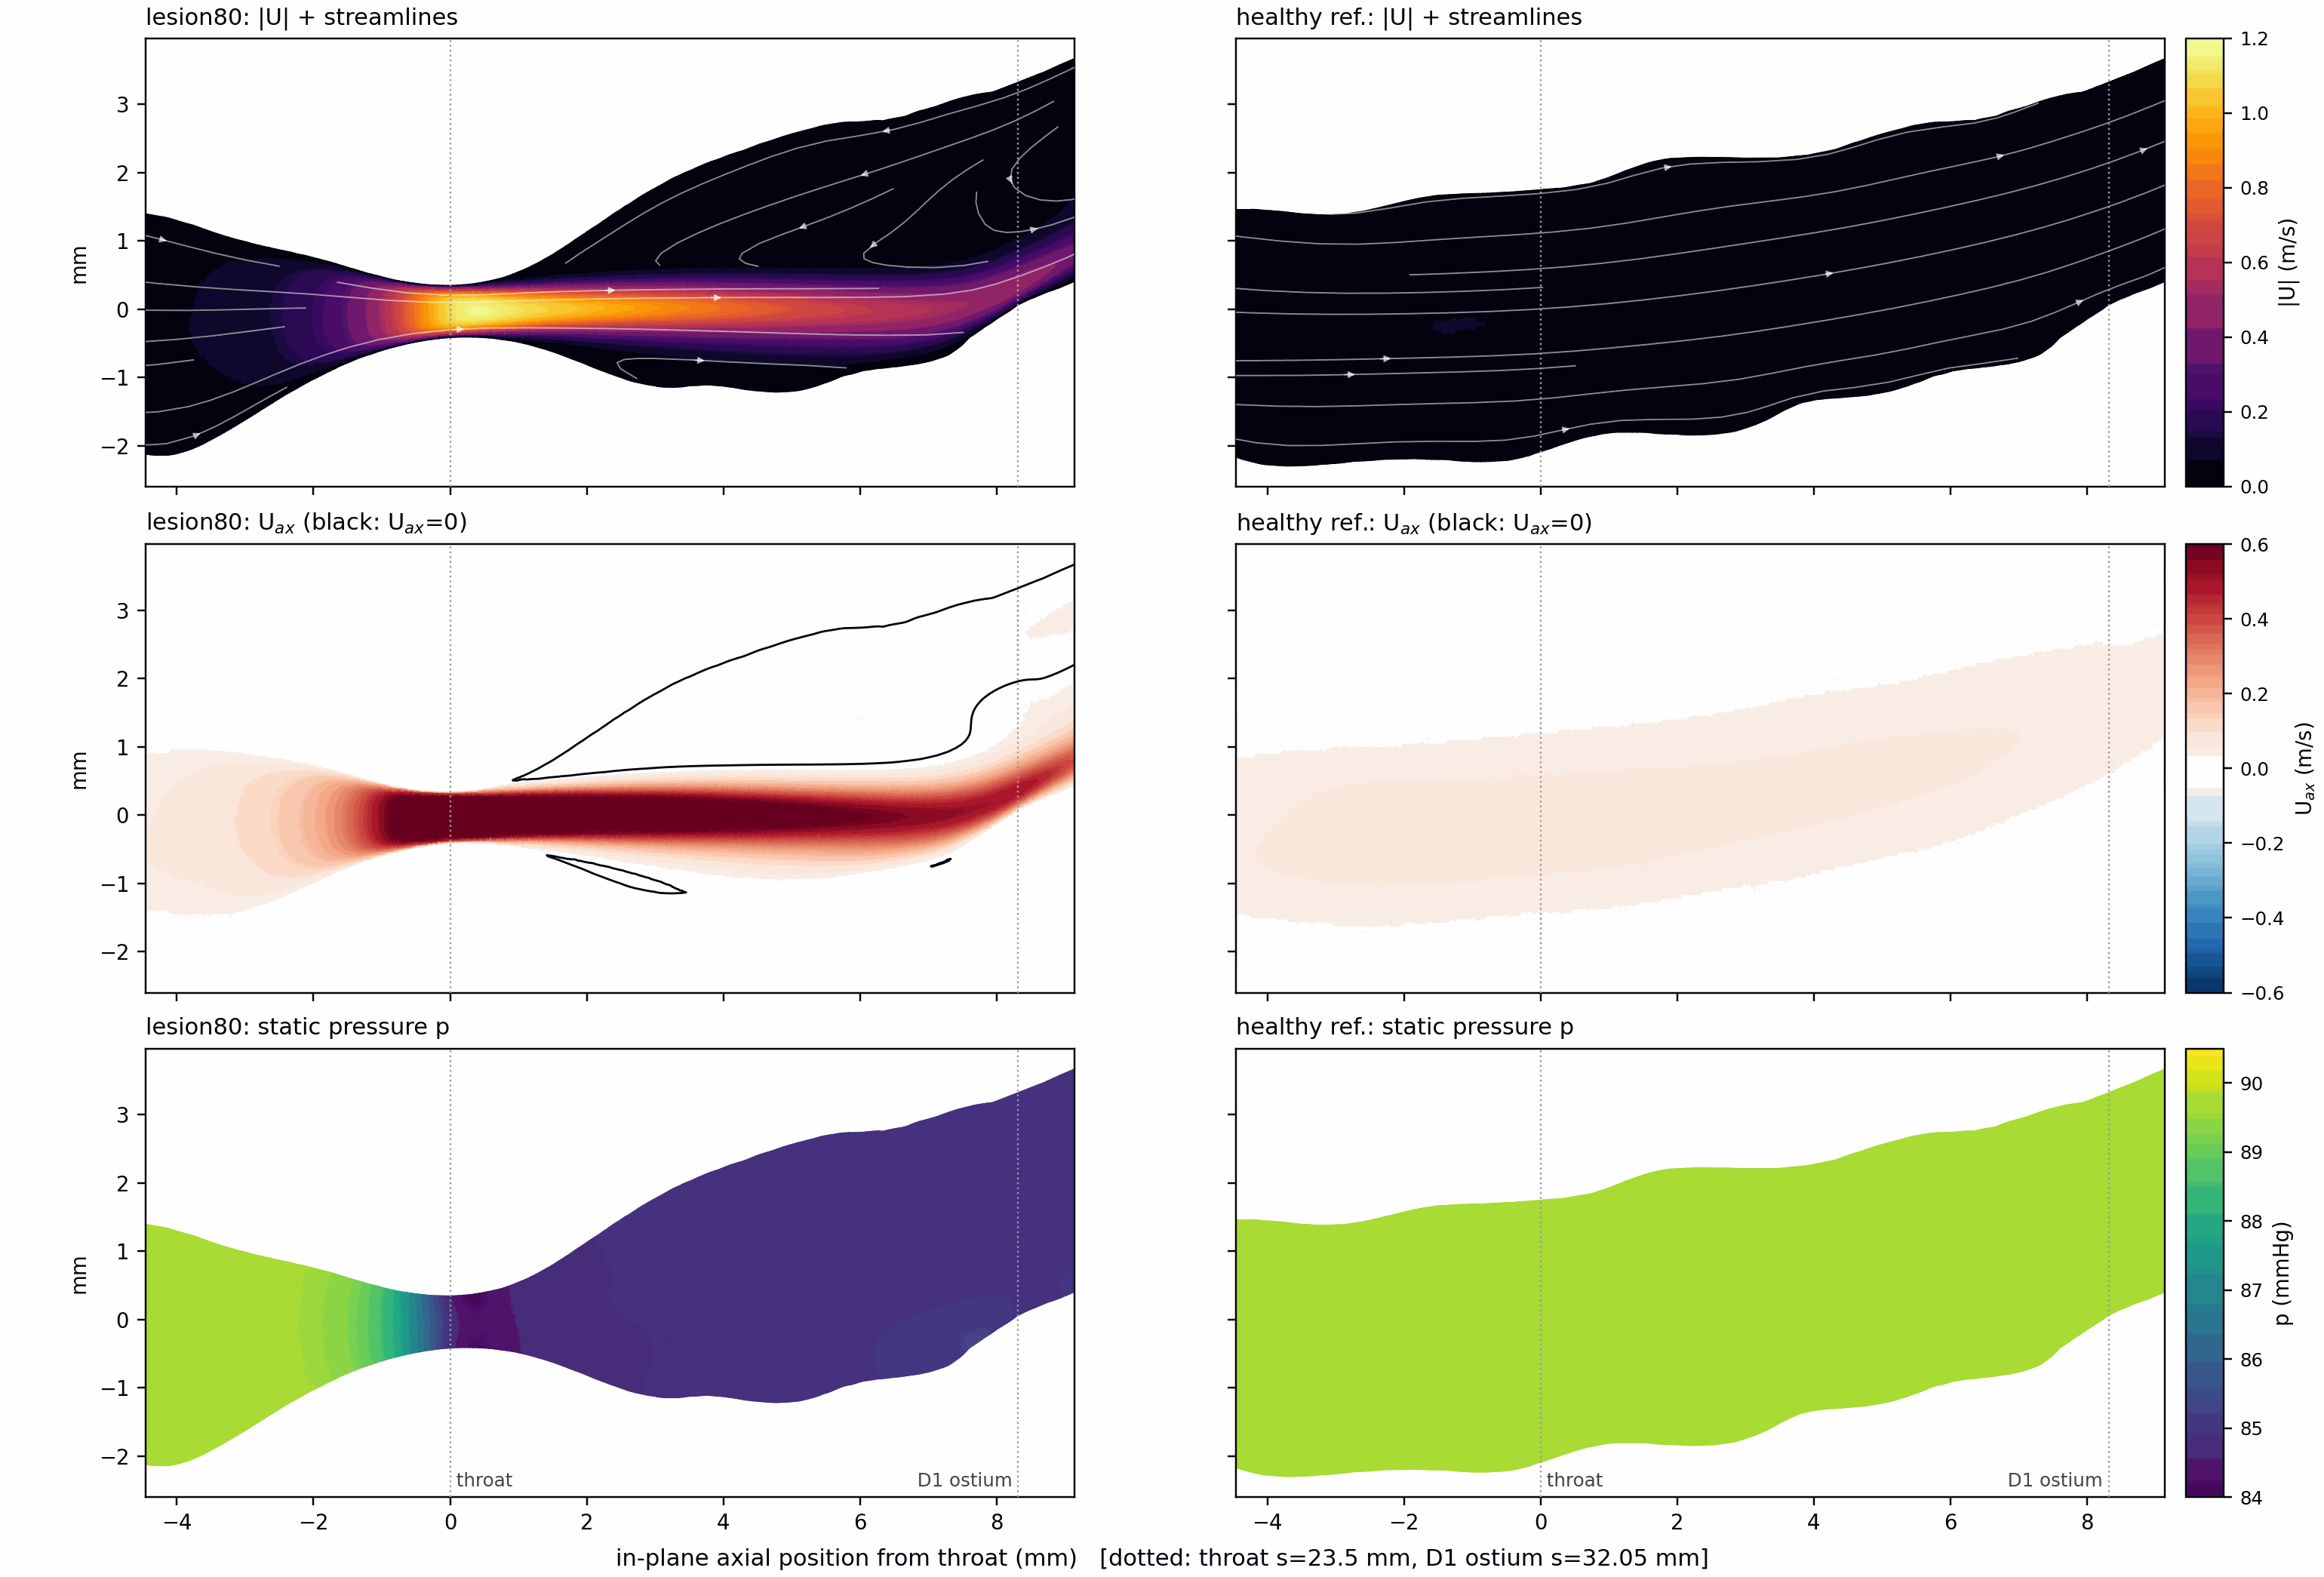
\includegraphics[width=\textwidth]{figures/cfd_longitudinal_throat.png}
\caption{As above, zoomed on the throat and the first 9\,mm downstream.}
\end{figure}

\begin{figure}[H]
\centering
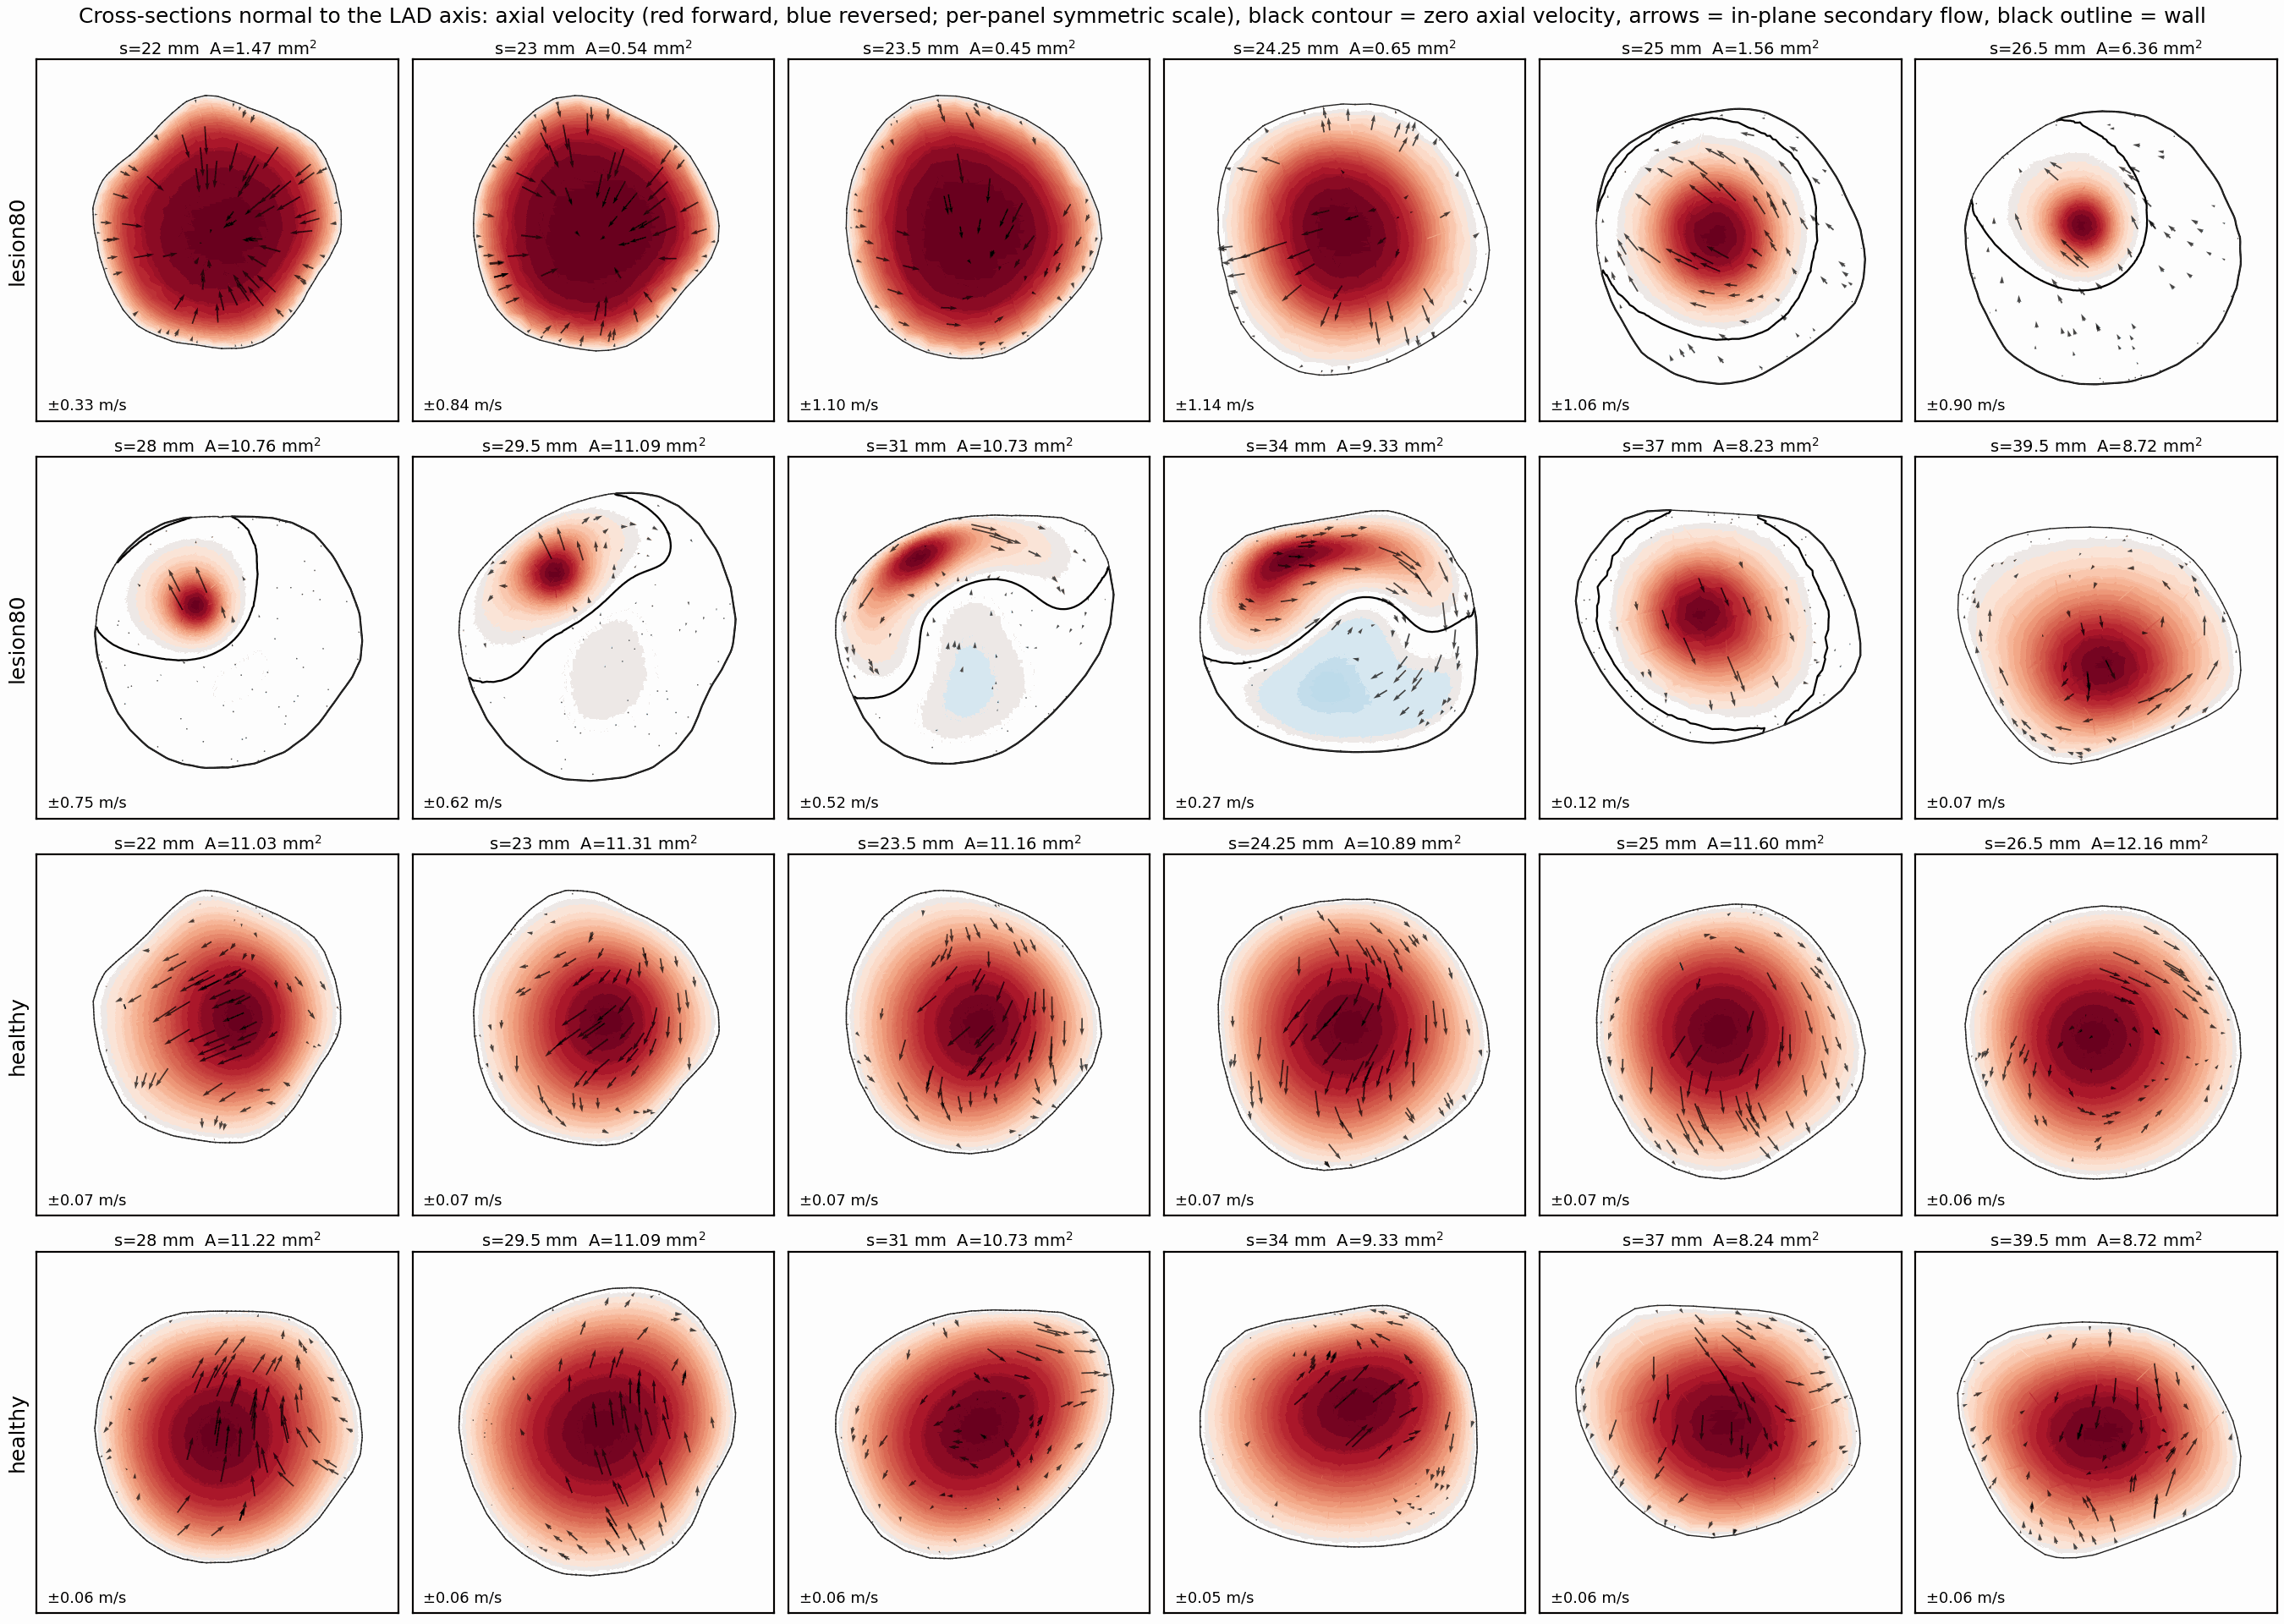
\includegraphics[width=\textwidth]{figures/cfd_cross_sections.png}
\caption{Cross-sections normal to the LAD axis at twelve stations (top two rows lesion80, bottom two rows healthy reference at the same stations): axial velocity (red forward, blue reversed, each panel on its own symmetric scale, stated in the corner), black = zero axial velocity (reversed-flow boundary), arrows = in-plane secondary flow, black outline = wall.
The jet fills the throat sections (peak axial velocity 1.10\,m/s at 23.5\,mm, area 0.45\,mm$^2$), becomes eccentric at 25\,mm (a crescent of reversed flow appears), and at 26.5--34\,mm forward flow is confined to a part of the section while 47--66\% of the area is reversed
(largest reversed velocity only $-0.04$ to $-0.07$\,m/s); at 37\,mm a thin reversed ring remains and at 39.5\,mm the flow is forward everywhere (peak 0.07\,m/s). The healthy sections show a smooth low-speed core with weak secondary flow.}
\end{figure}

\begin{figure}[H]
\centering
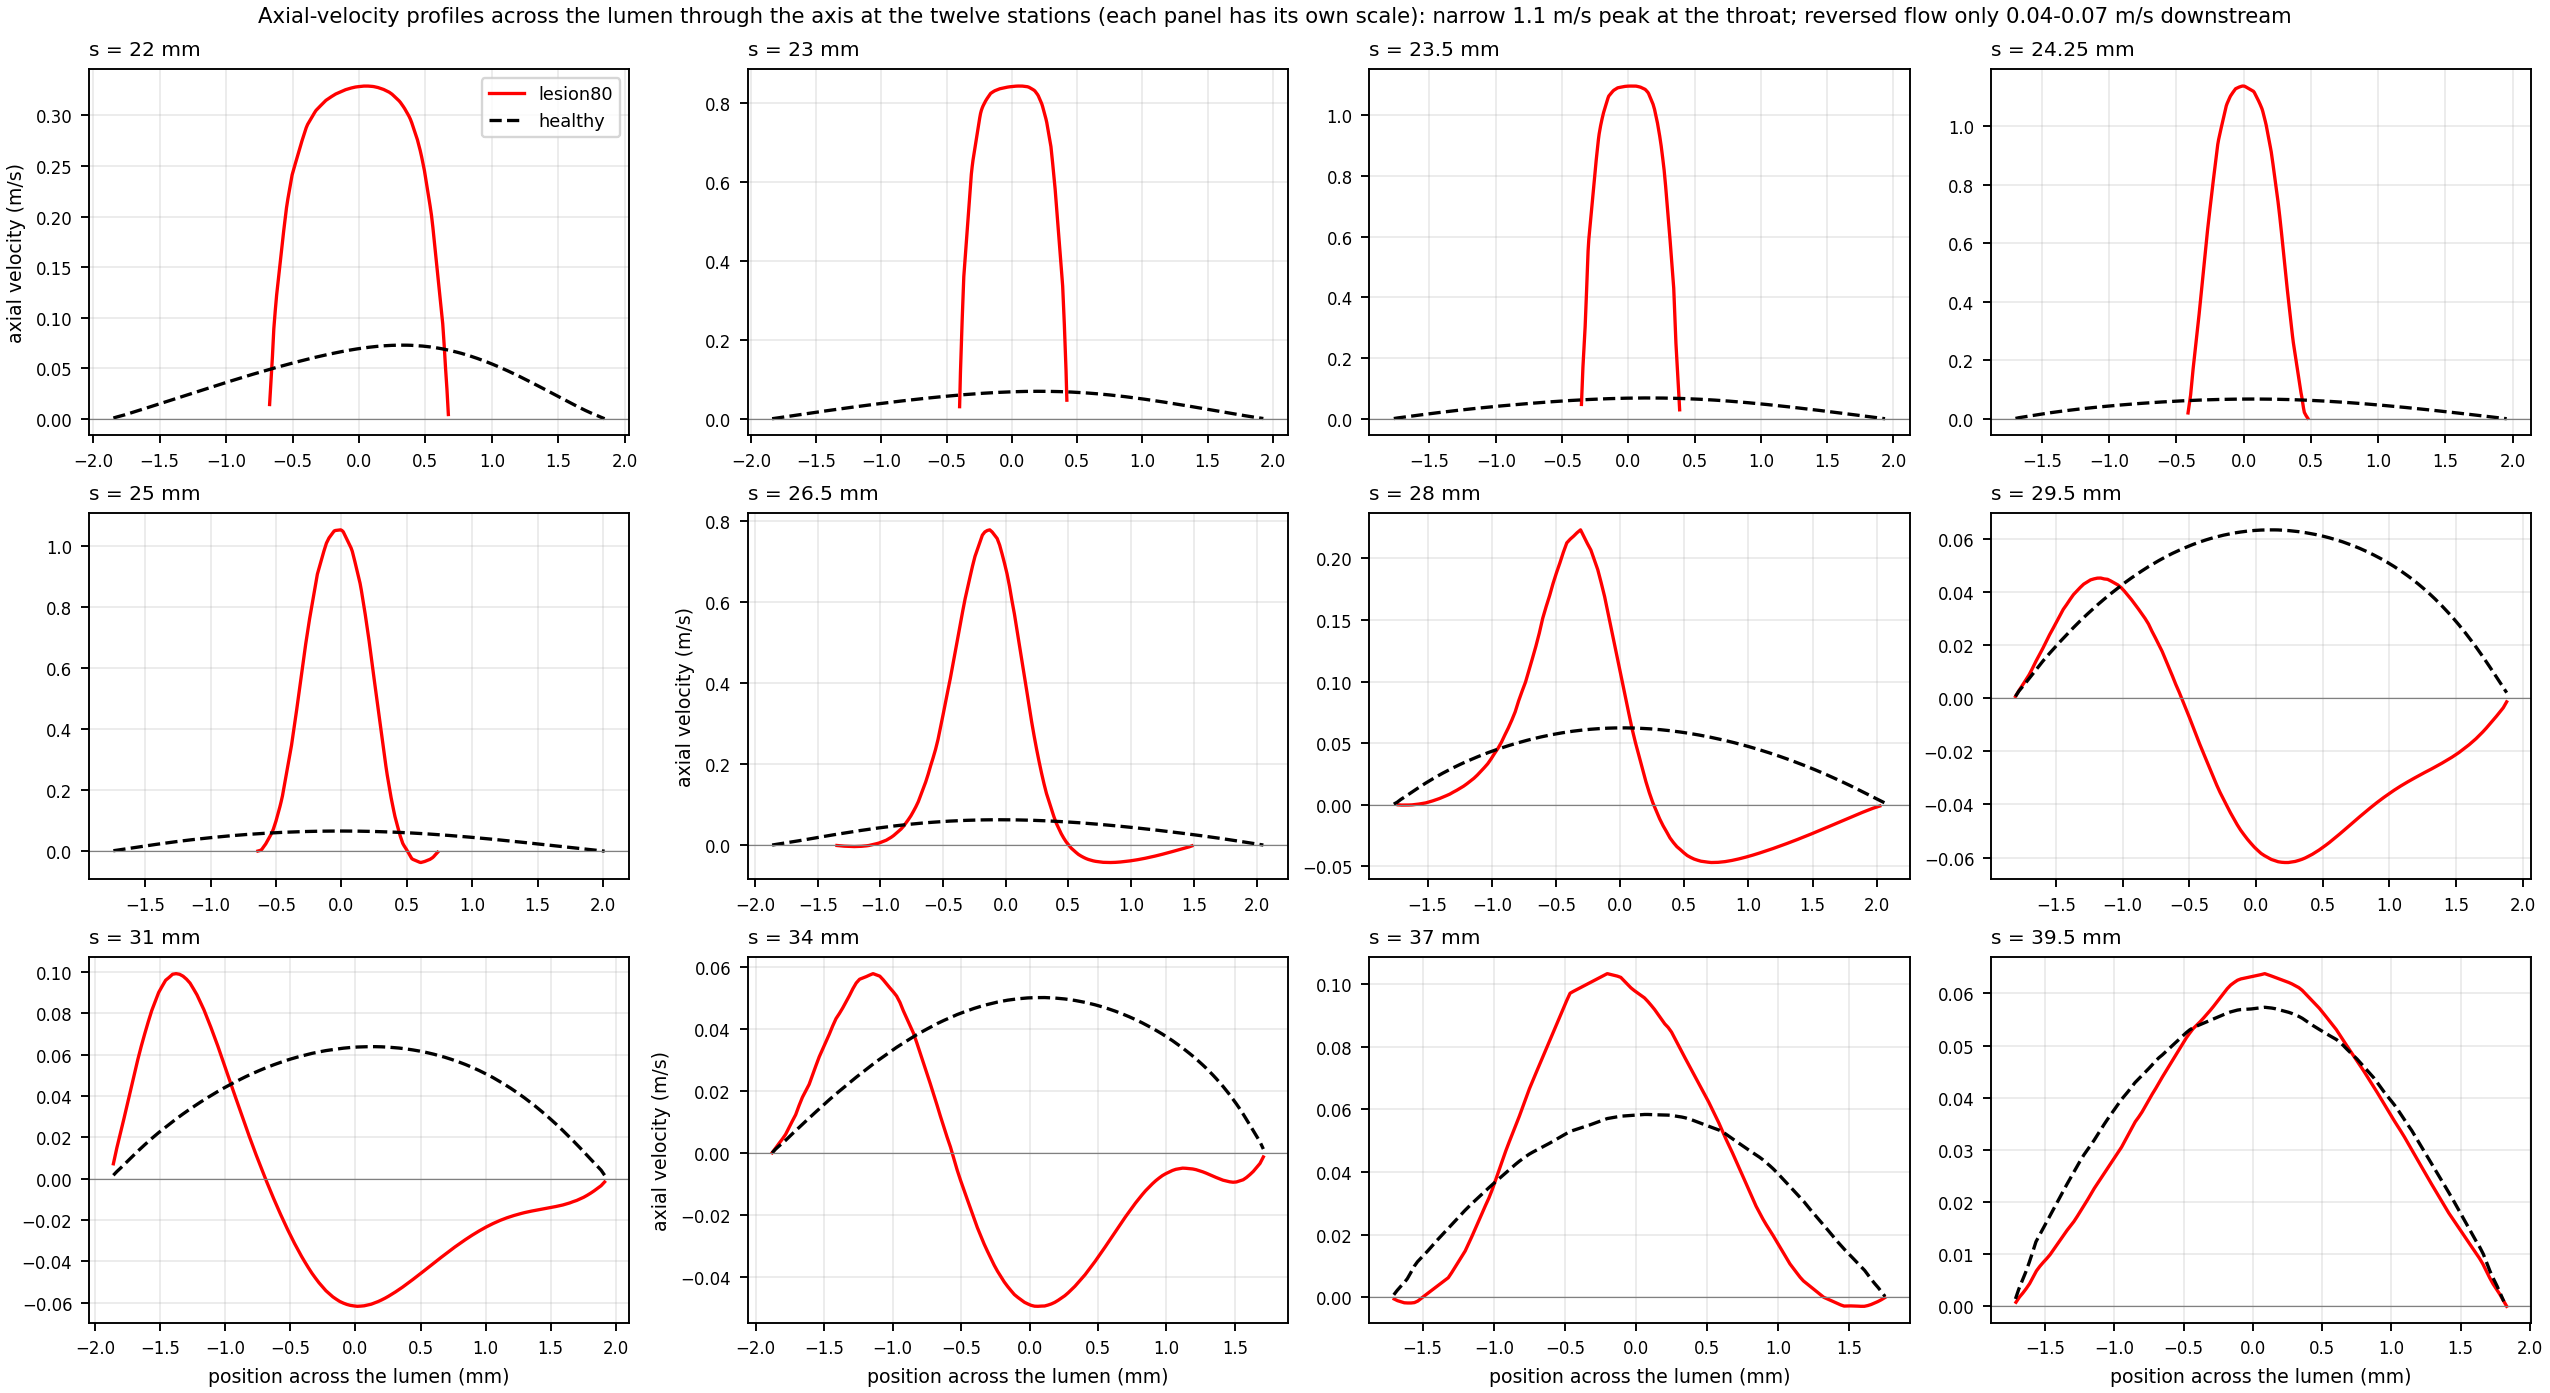
\includegraphics[width=\textwidth]{figures/cfd_velocity_profiles.png}
\caption{Axial-velocity profiles across the lumen (through the axis, in-plane direction) at the twelve stations, lesion80 (red) against the healthy reference (black dashed), each panel on its own scale. The throat profile is a narrow peak of 1.1\,m/s in a 0.75\,mm lumen; downstream the jet decays and moves off-axis, and the reversed flow (negative values) reaches only $-0.04$ to $-0.07$\,m/s
(stations 25--34\,mm); by 39.5\,mm the lesion profile has returned to the healthy shape.}
\end{figure}

\begin{figure}[H]
\centering
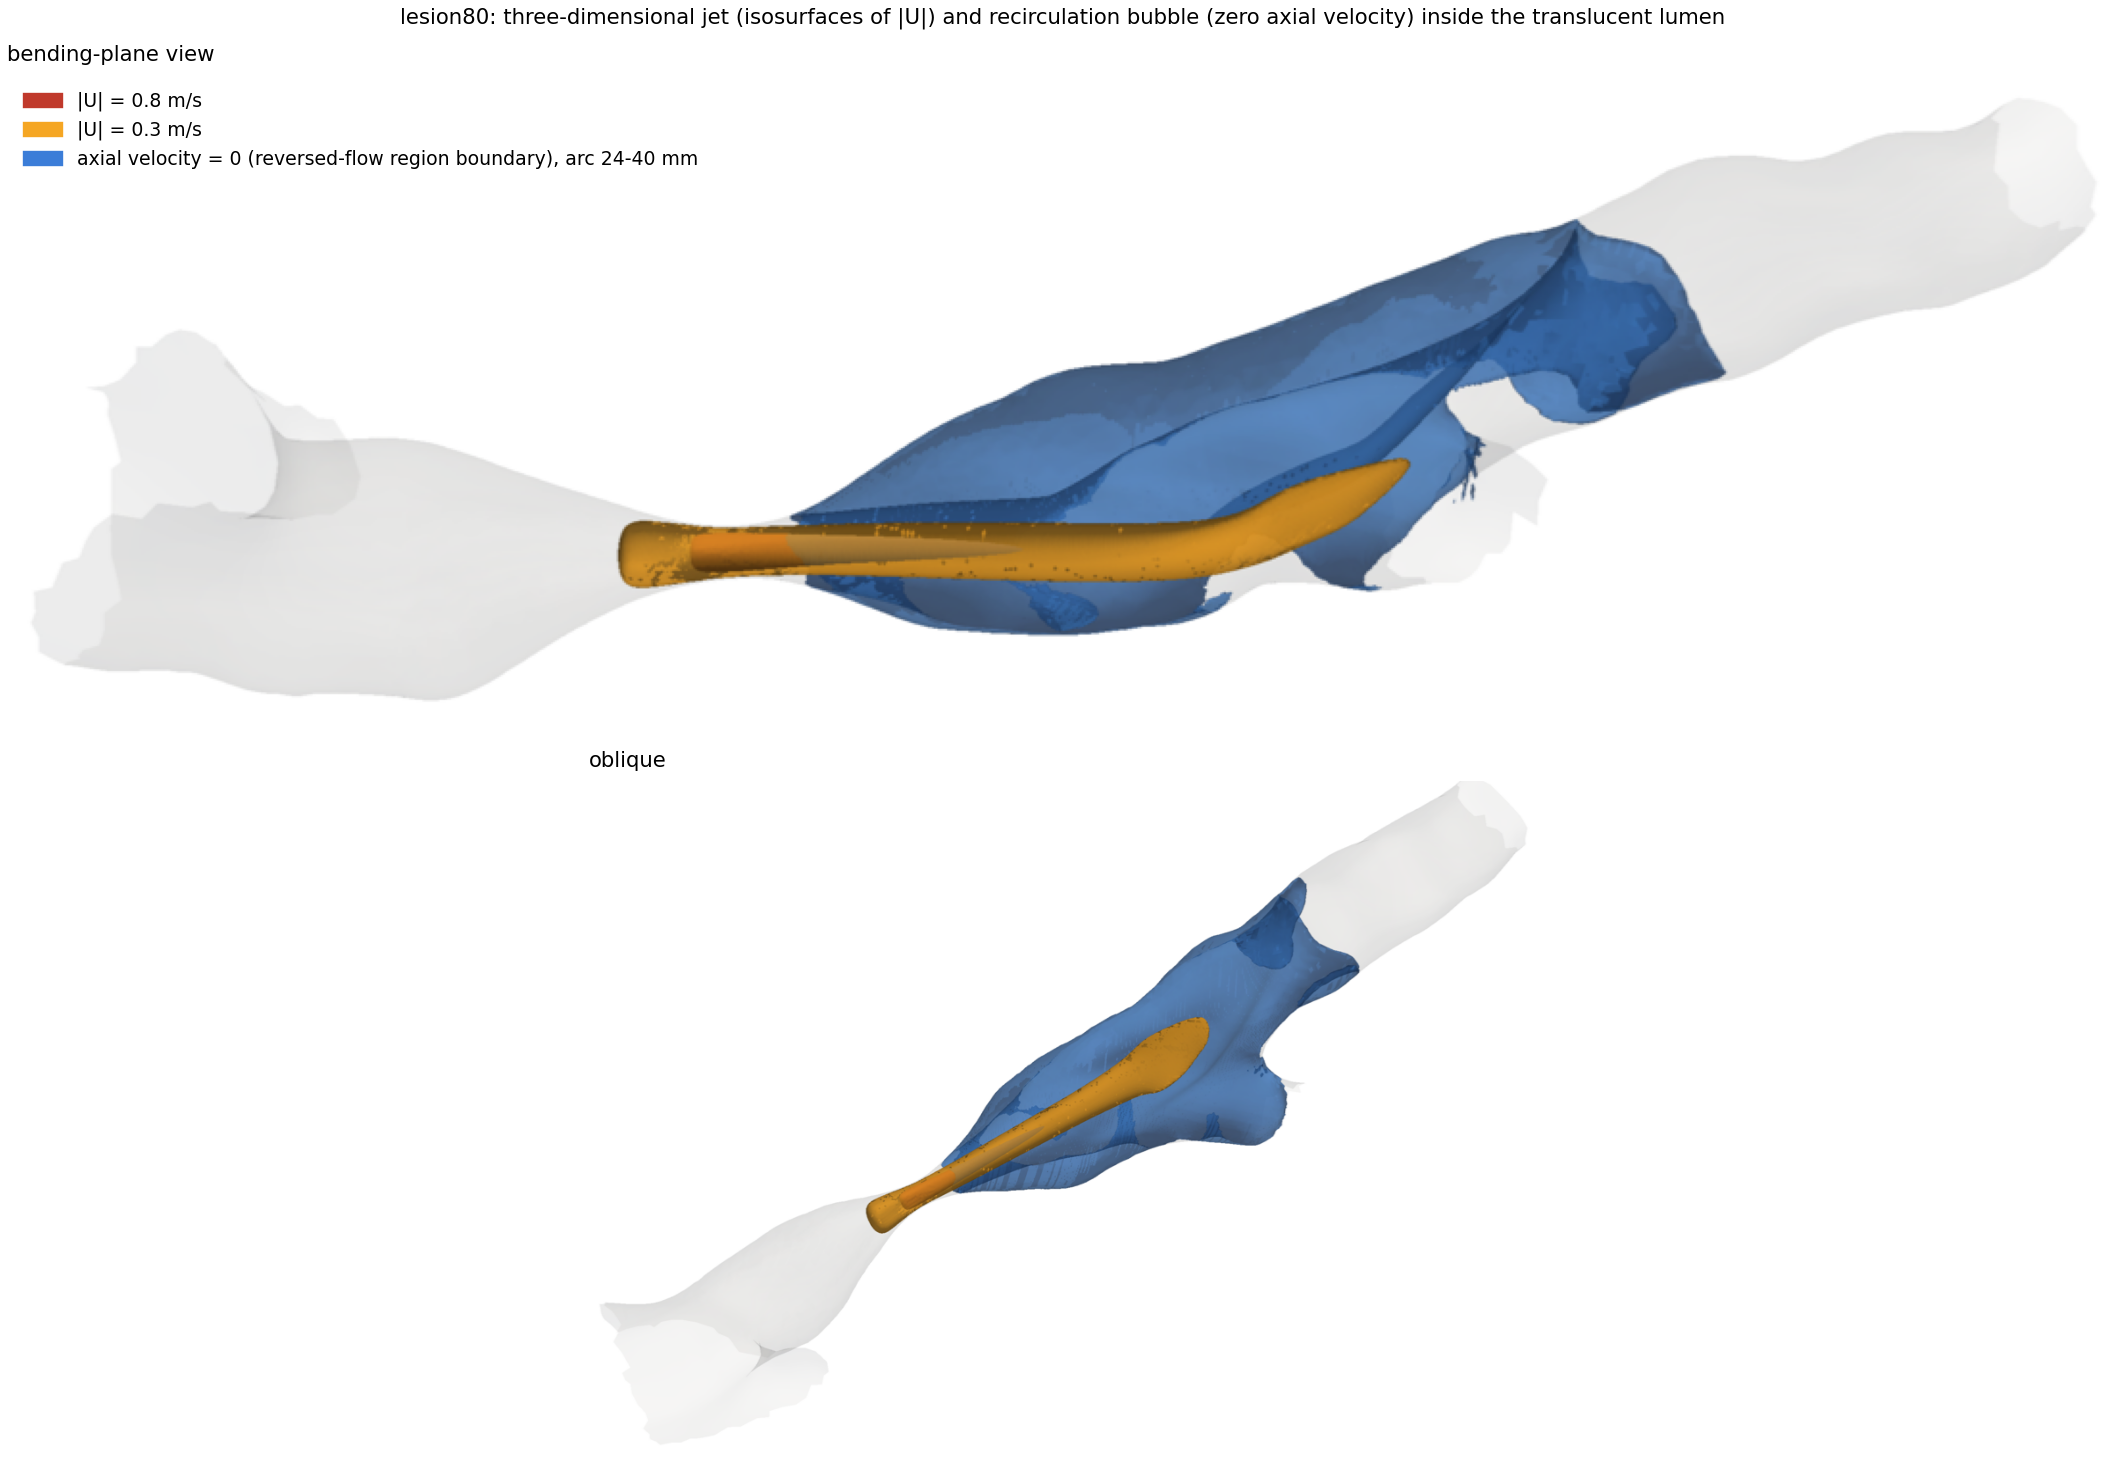
\includegraphics[width=\textwidth]{figures/cfd_jet_bubble_3d.png}
\caption{Lesion80, three-dimensional structure of the flow: isosurfaces of $|U|=0.3$\,m/s (orange) and $0.8$\,m/s (red) show the jet leaving the throat as a slender core that bends towards the wall; the blue surface is the zero-axial-velocity surface for arc 24--40\,mm and encloses the recirculation region, which wraps around the jet
(it touches the wall over much of its extent). Two views; translucent grey: lumen.}
\end{figure}

\begin{figure}[H]
\centering
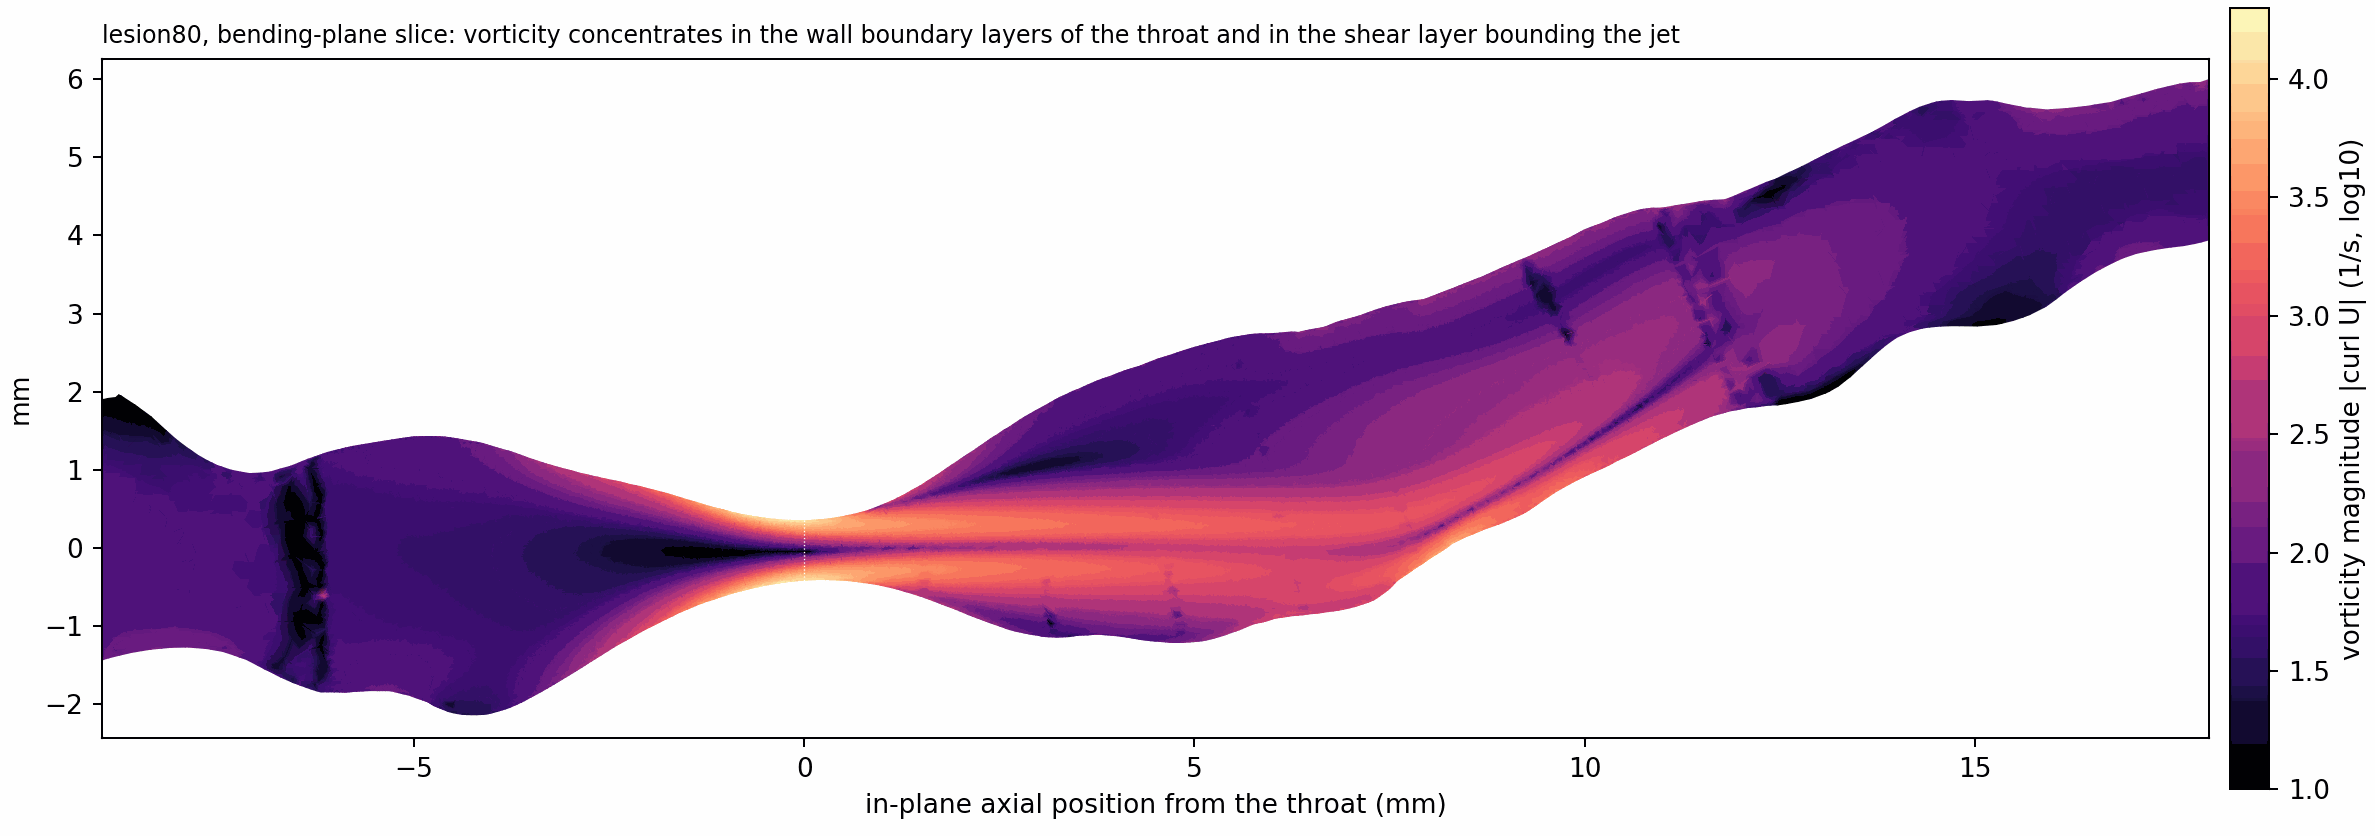
\includegraphics[width=\textwidth]{figures/cfd_vorticity_slice.png}
\caption{Vorticity magnitude $|\nabla\times\mathbf U|$ on the bending-plane slice of lesion80 (log$_{10}$, 1/s): the throat wall boundary layers ($\gtrsim10^{4}$\,1/s) and the thin shear layer bounding the jet stand out against the low-vorticity recirculation. The thin dark streaks crossing the vessel (at about $-6.5$, $3$--$4$ and $9$--$12$\,mm)
are artefacts of the velocity-gradient computation across mesh-refinement interfaces, not flow features.}
\end{figure}

\begin{figure}[H]
\centering
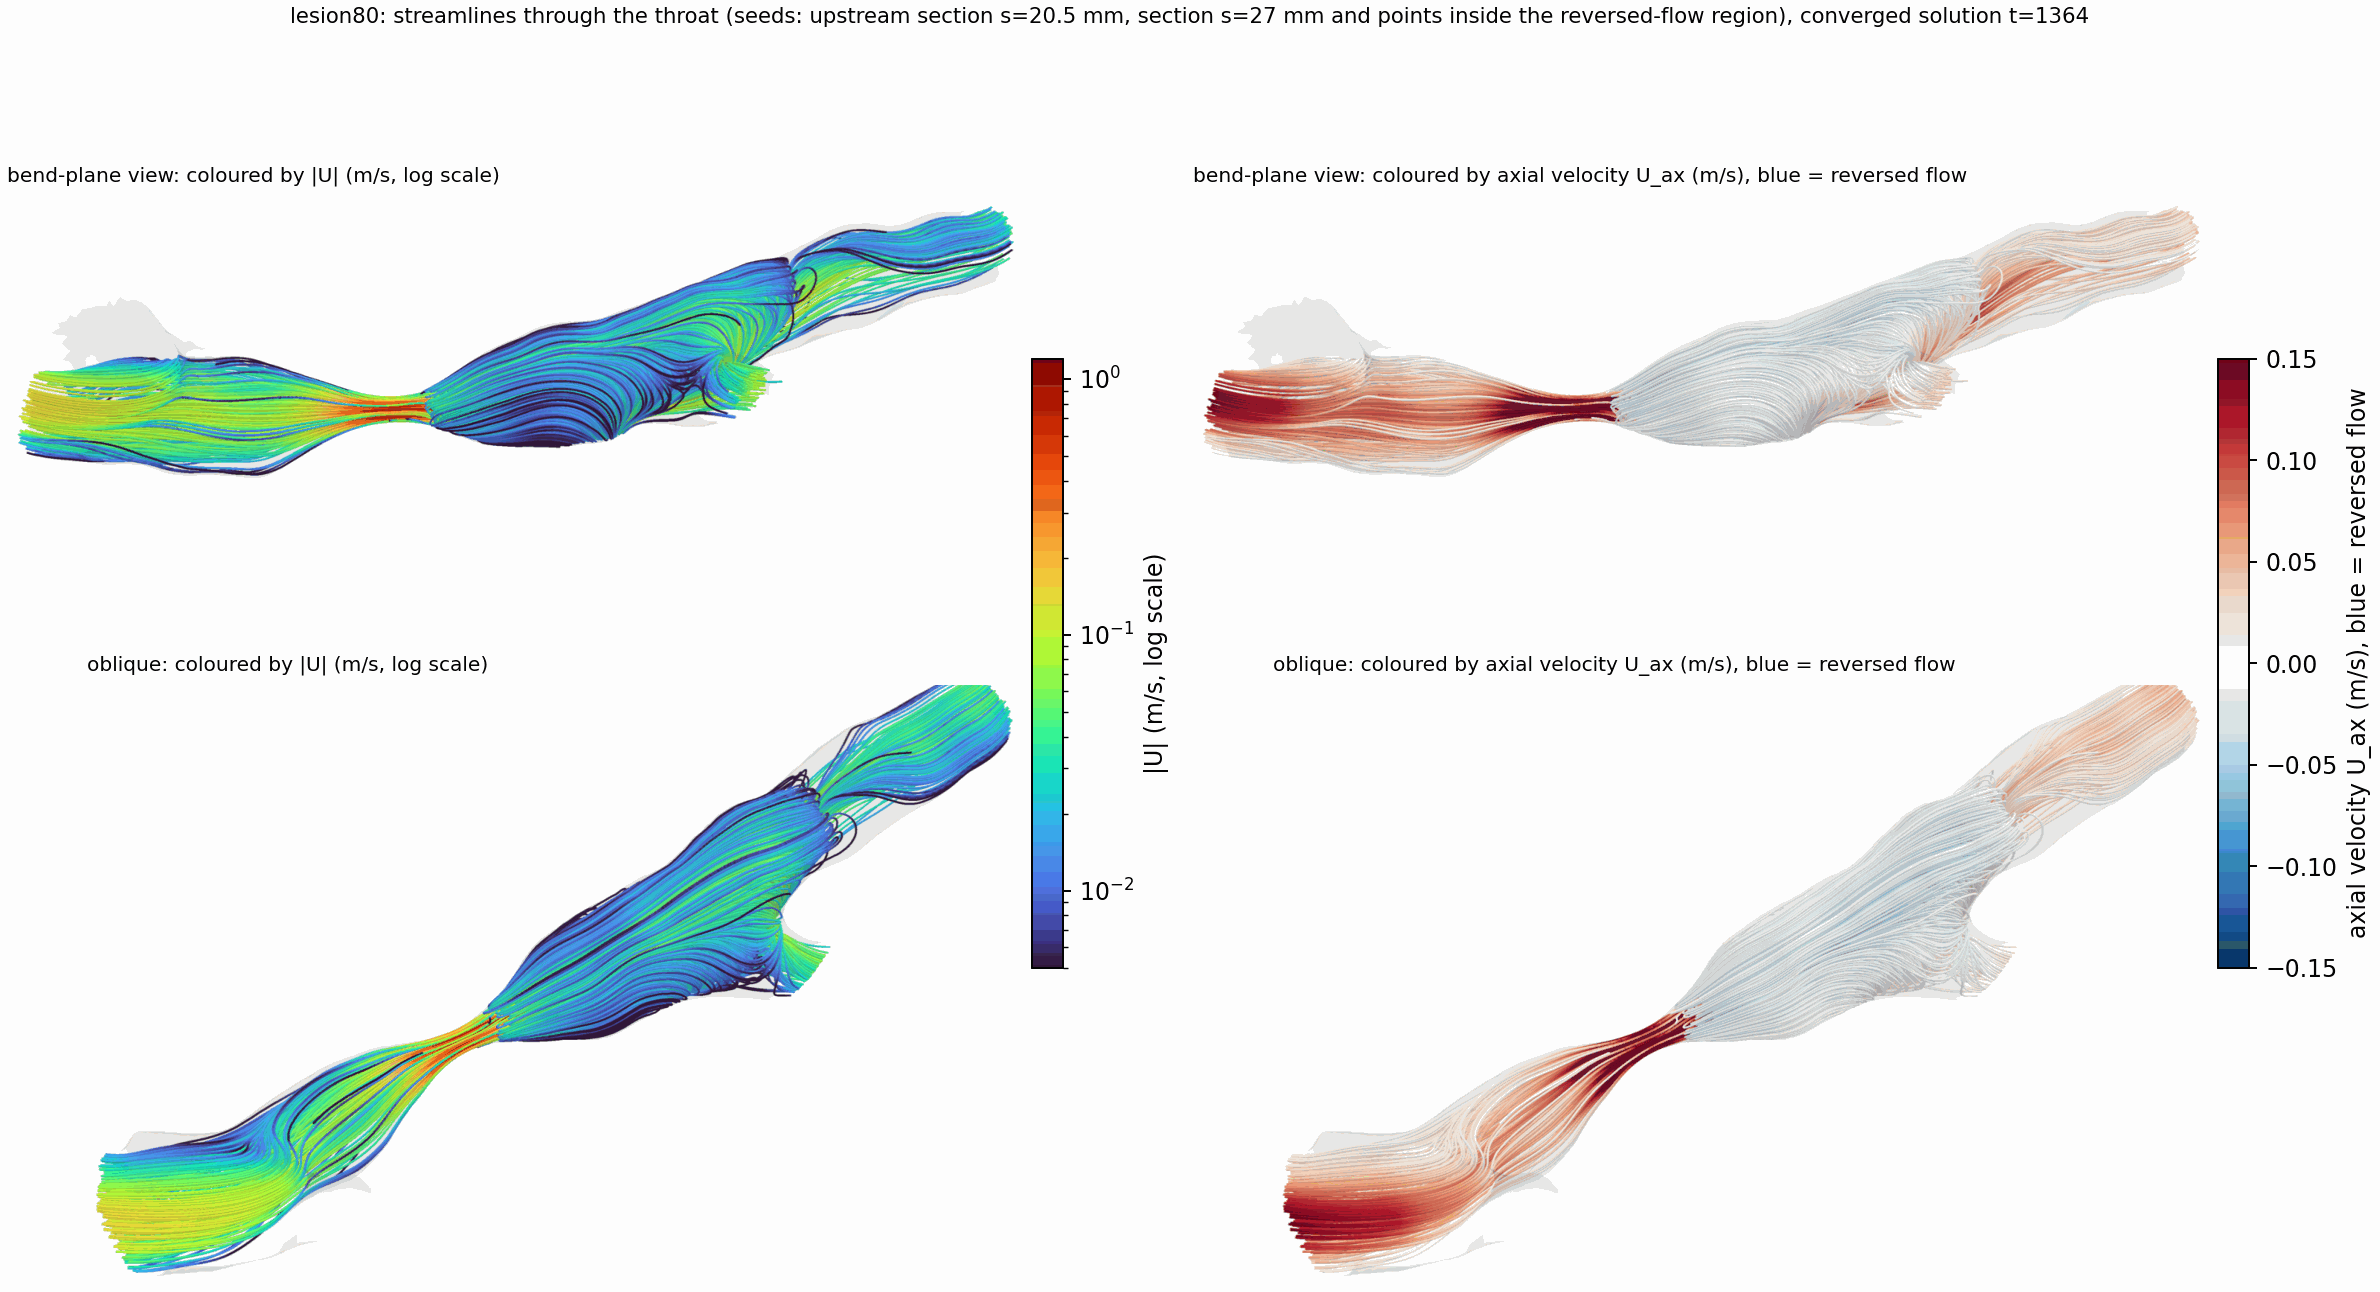
\includegraphics[width=\textwidth]{figures/cfd_streamlines_3d.png}
\caption{Streamlines through the stenosis (lesion80; seeds on the upstream section at arc 20.5\,mm, on the section at 27\,mm and inside the reversed-flow region): left coloured by $|U|$ (logarithmic scale; the jet is the red/orange core, the recirculating flow moves at 0.005--0.05\,m/s),
right coloured by axial velocity on a $\pm0.15$\,m/s scale (blue = reversed). Two views.}
\end{figure}

\begin{figure}[H]
\centering
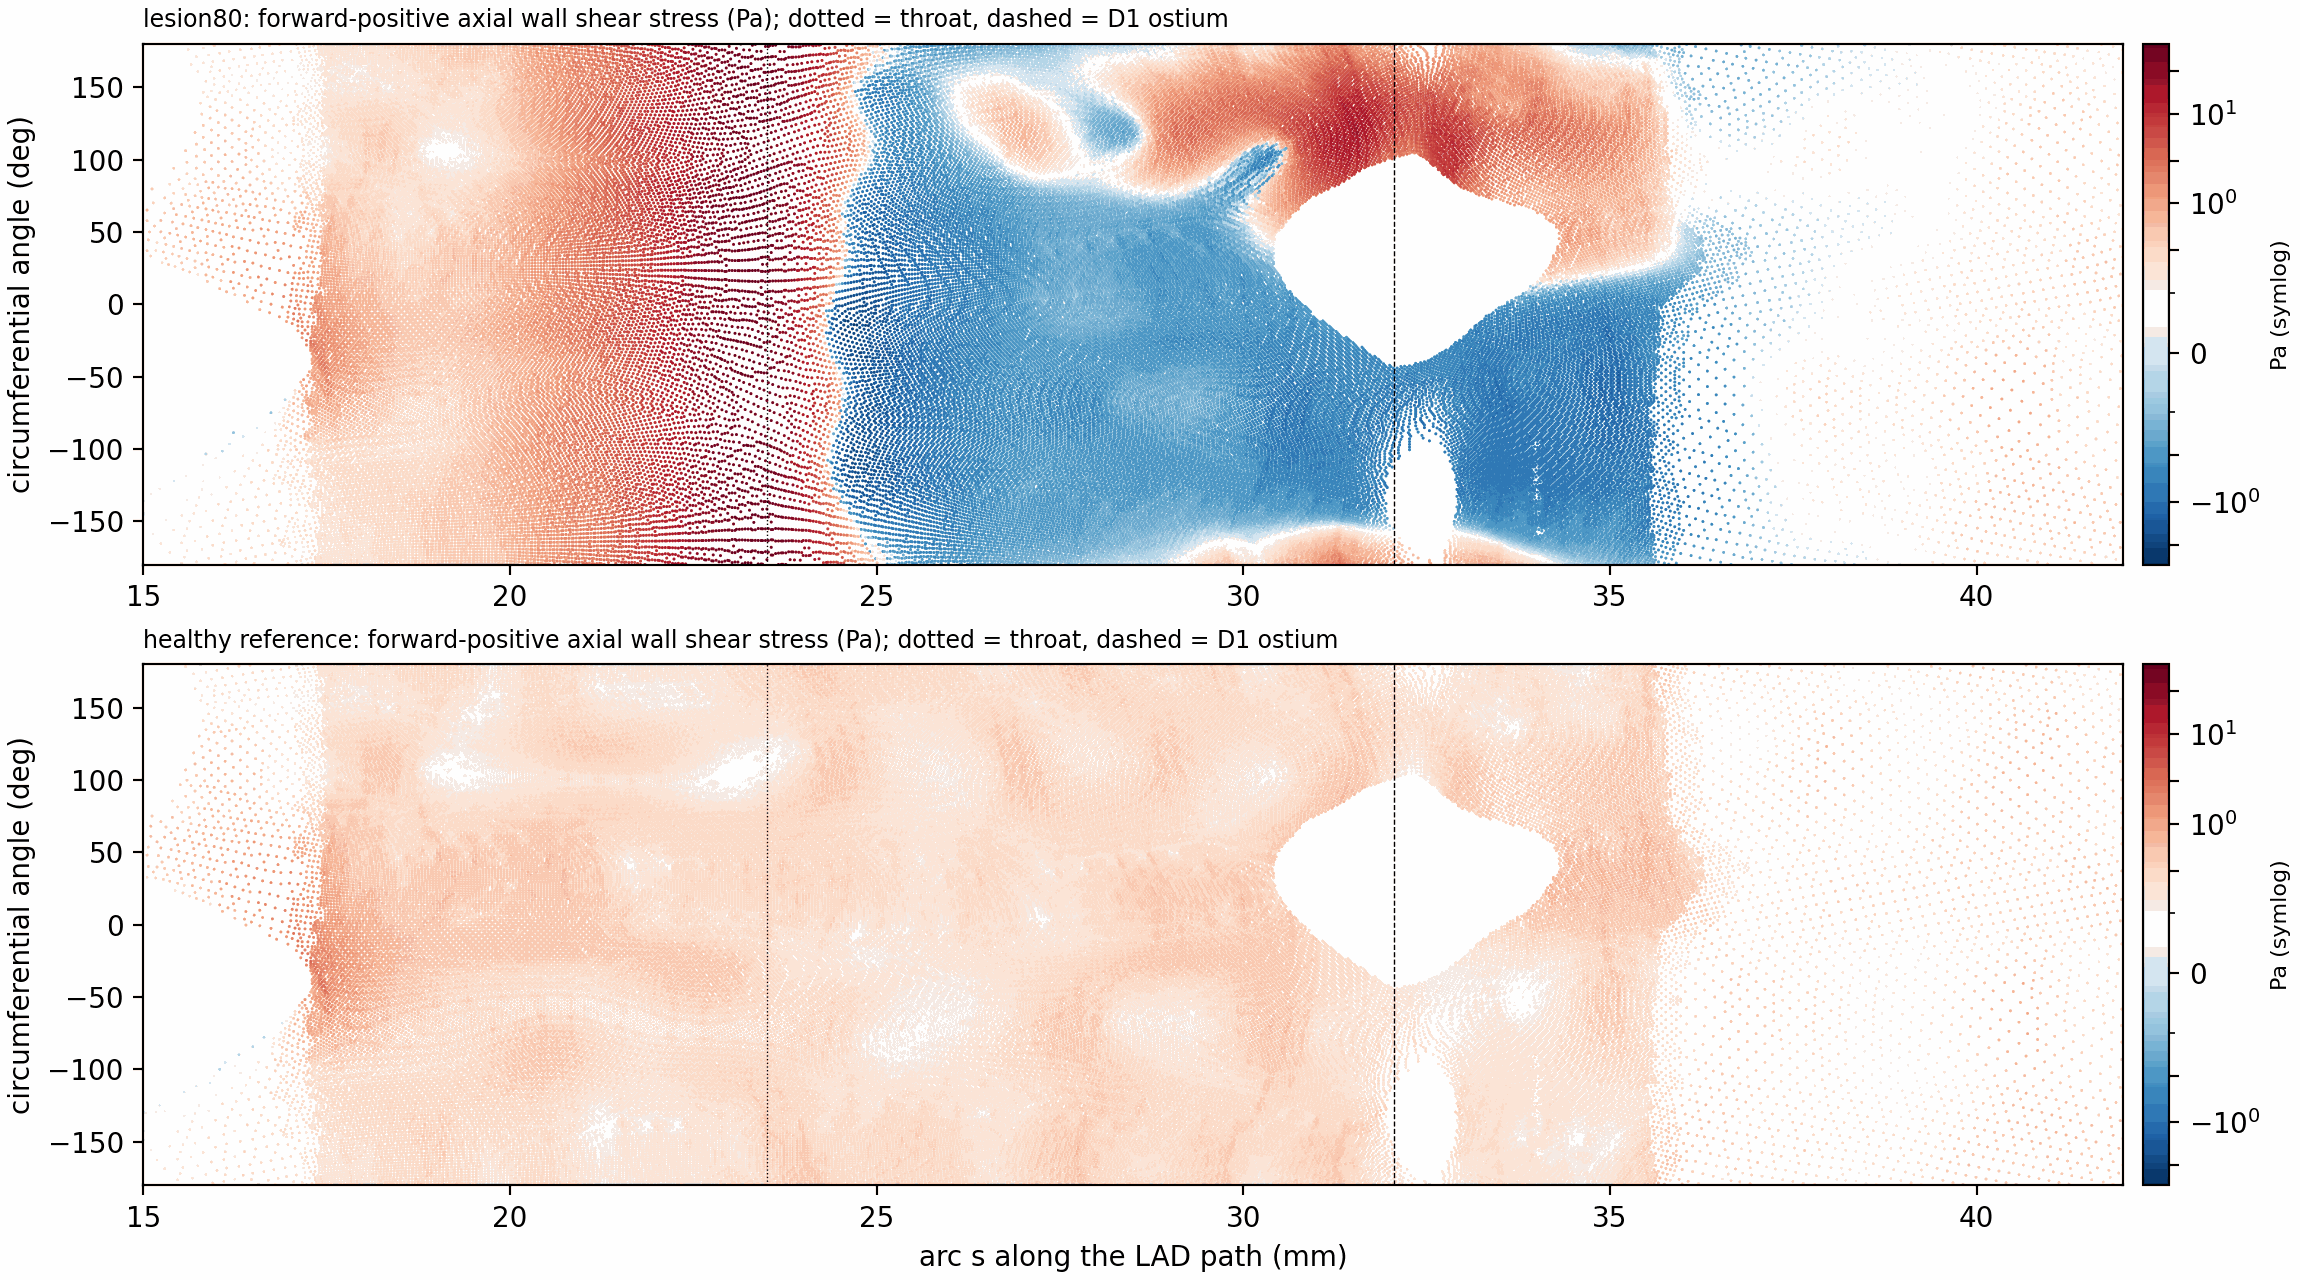
\includegraphics[width=\textwidth]{figures/cfd_wss_unrolled.png}
\caption{Wall shear stress unrolled onto arc length and circumferential angle (LAD-path wall faces only; forward-positive axial component, symmetric-logarithmic colour scale). Lesion80: forward shear rises to $\approx$51\,Pa at the throat; from arc $\approx$24.5\,mm to $\approx$35.7\,mm the wall shear is reversed over almost the whole circumference
(blue), except a forward band on the side facing the D1 ostium (white gap: D1 wall faces, not part of the LAD path); weakly reversed patches continue to $\approx$38--39\,mm. Healthy reference: uniform forward shear of 0.2--0.4\,Pa.}
\end{figure}

\begin{figure}[H]
\centering
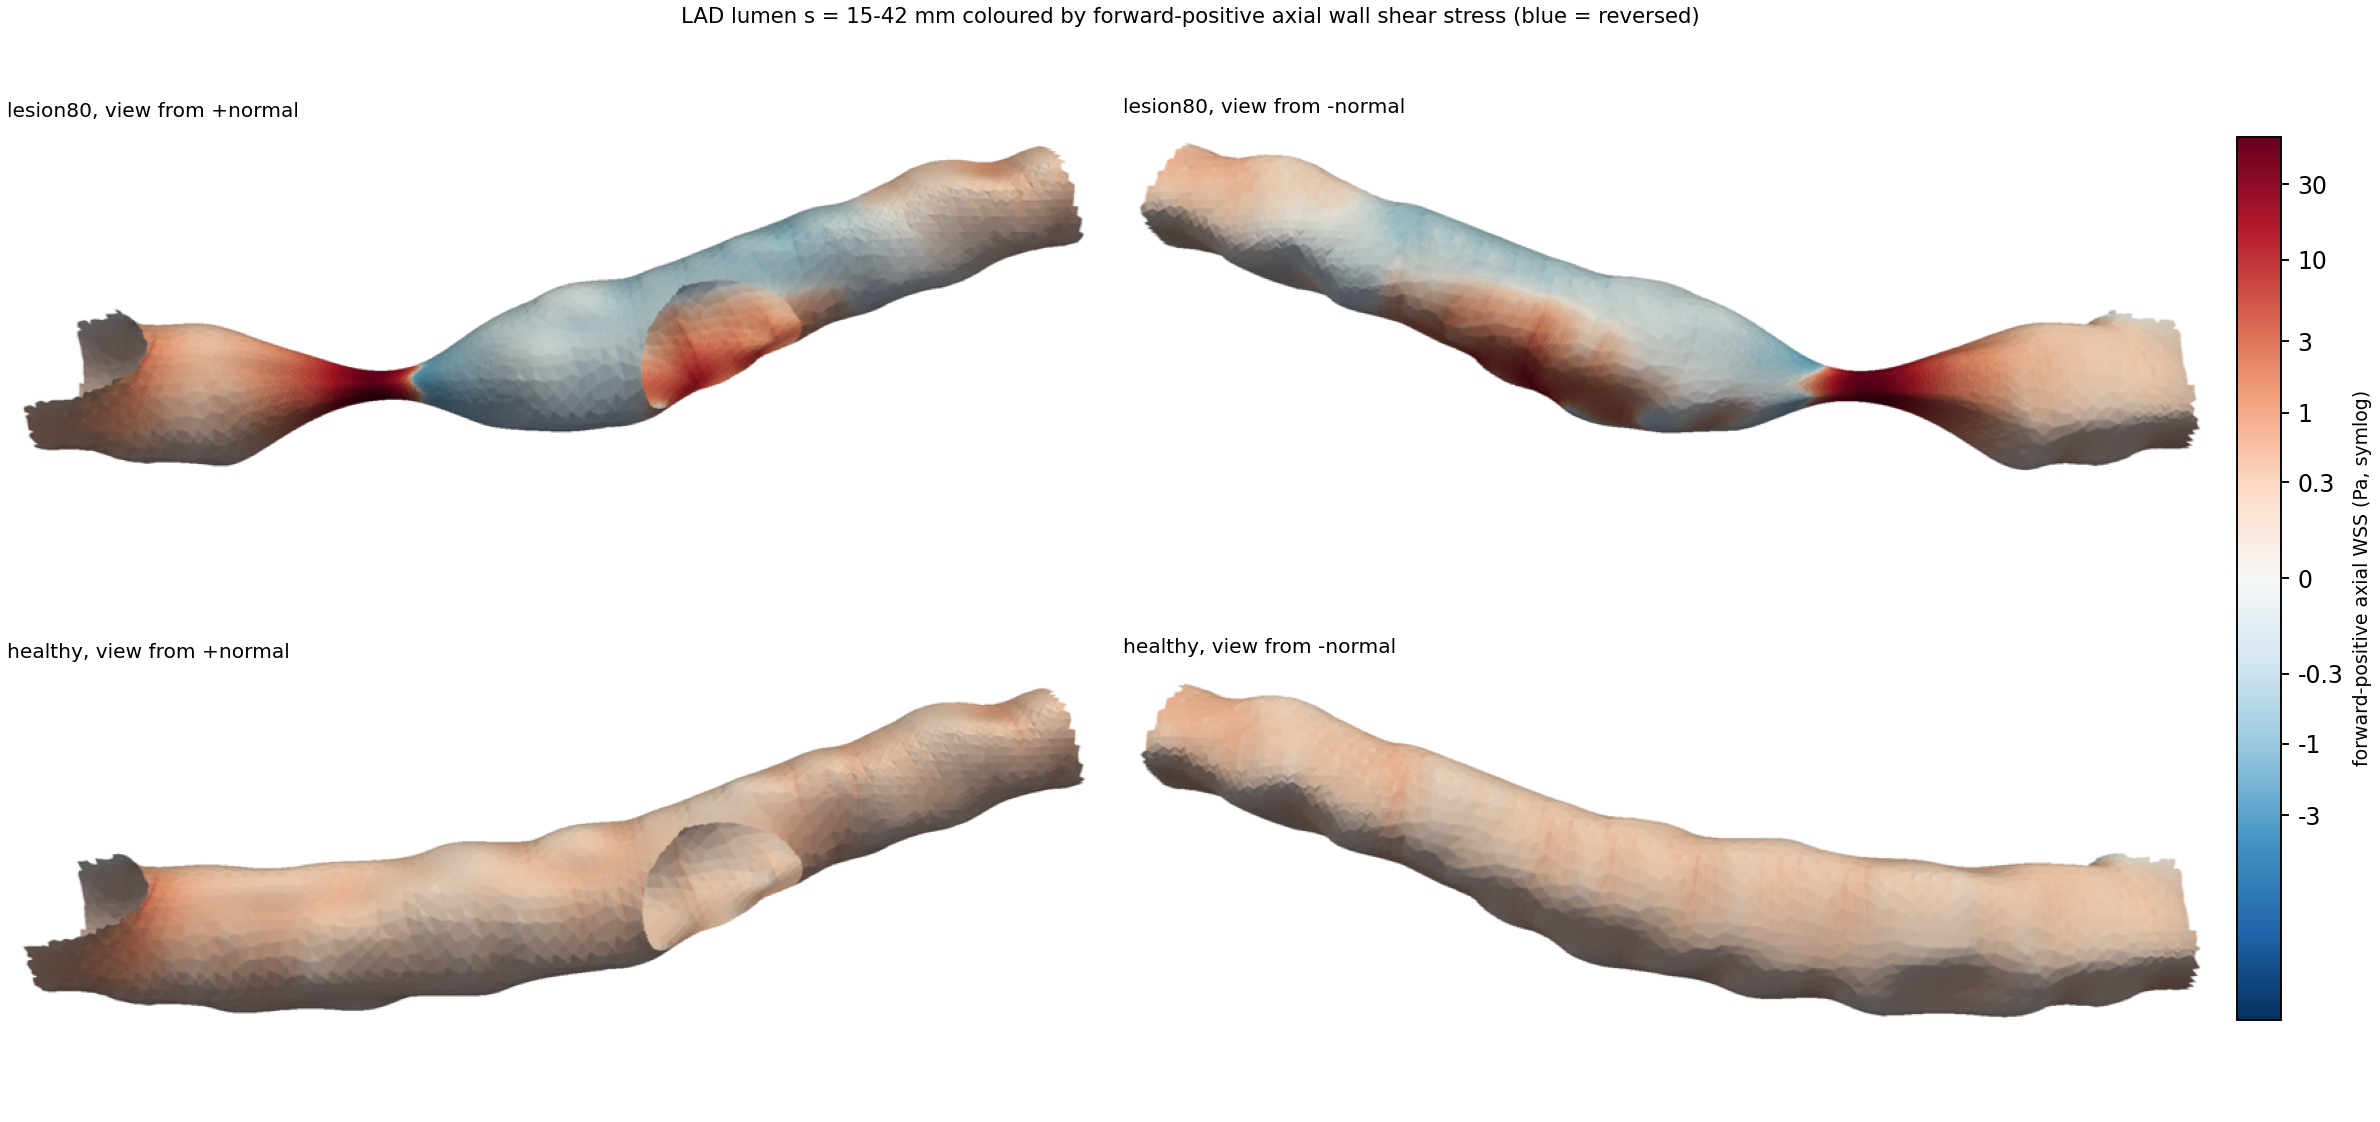
\includegraphics[width=\textwidth]{figures/cfd_wss_3d.png}
\caption{The same wall shear stress on the 3D lumen of the LAD (arc 15--42\,mm), viewed from the two sides of the bending plane. Lesion80 top, healthy reference bottom.}
\end{figure}

\begin{figure}[H]
\centering
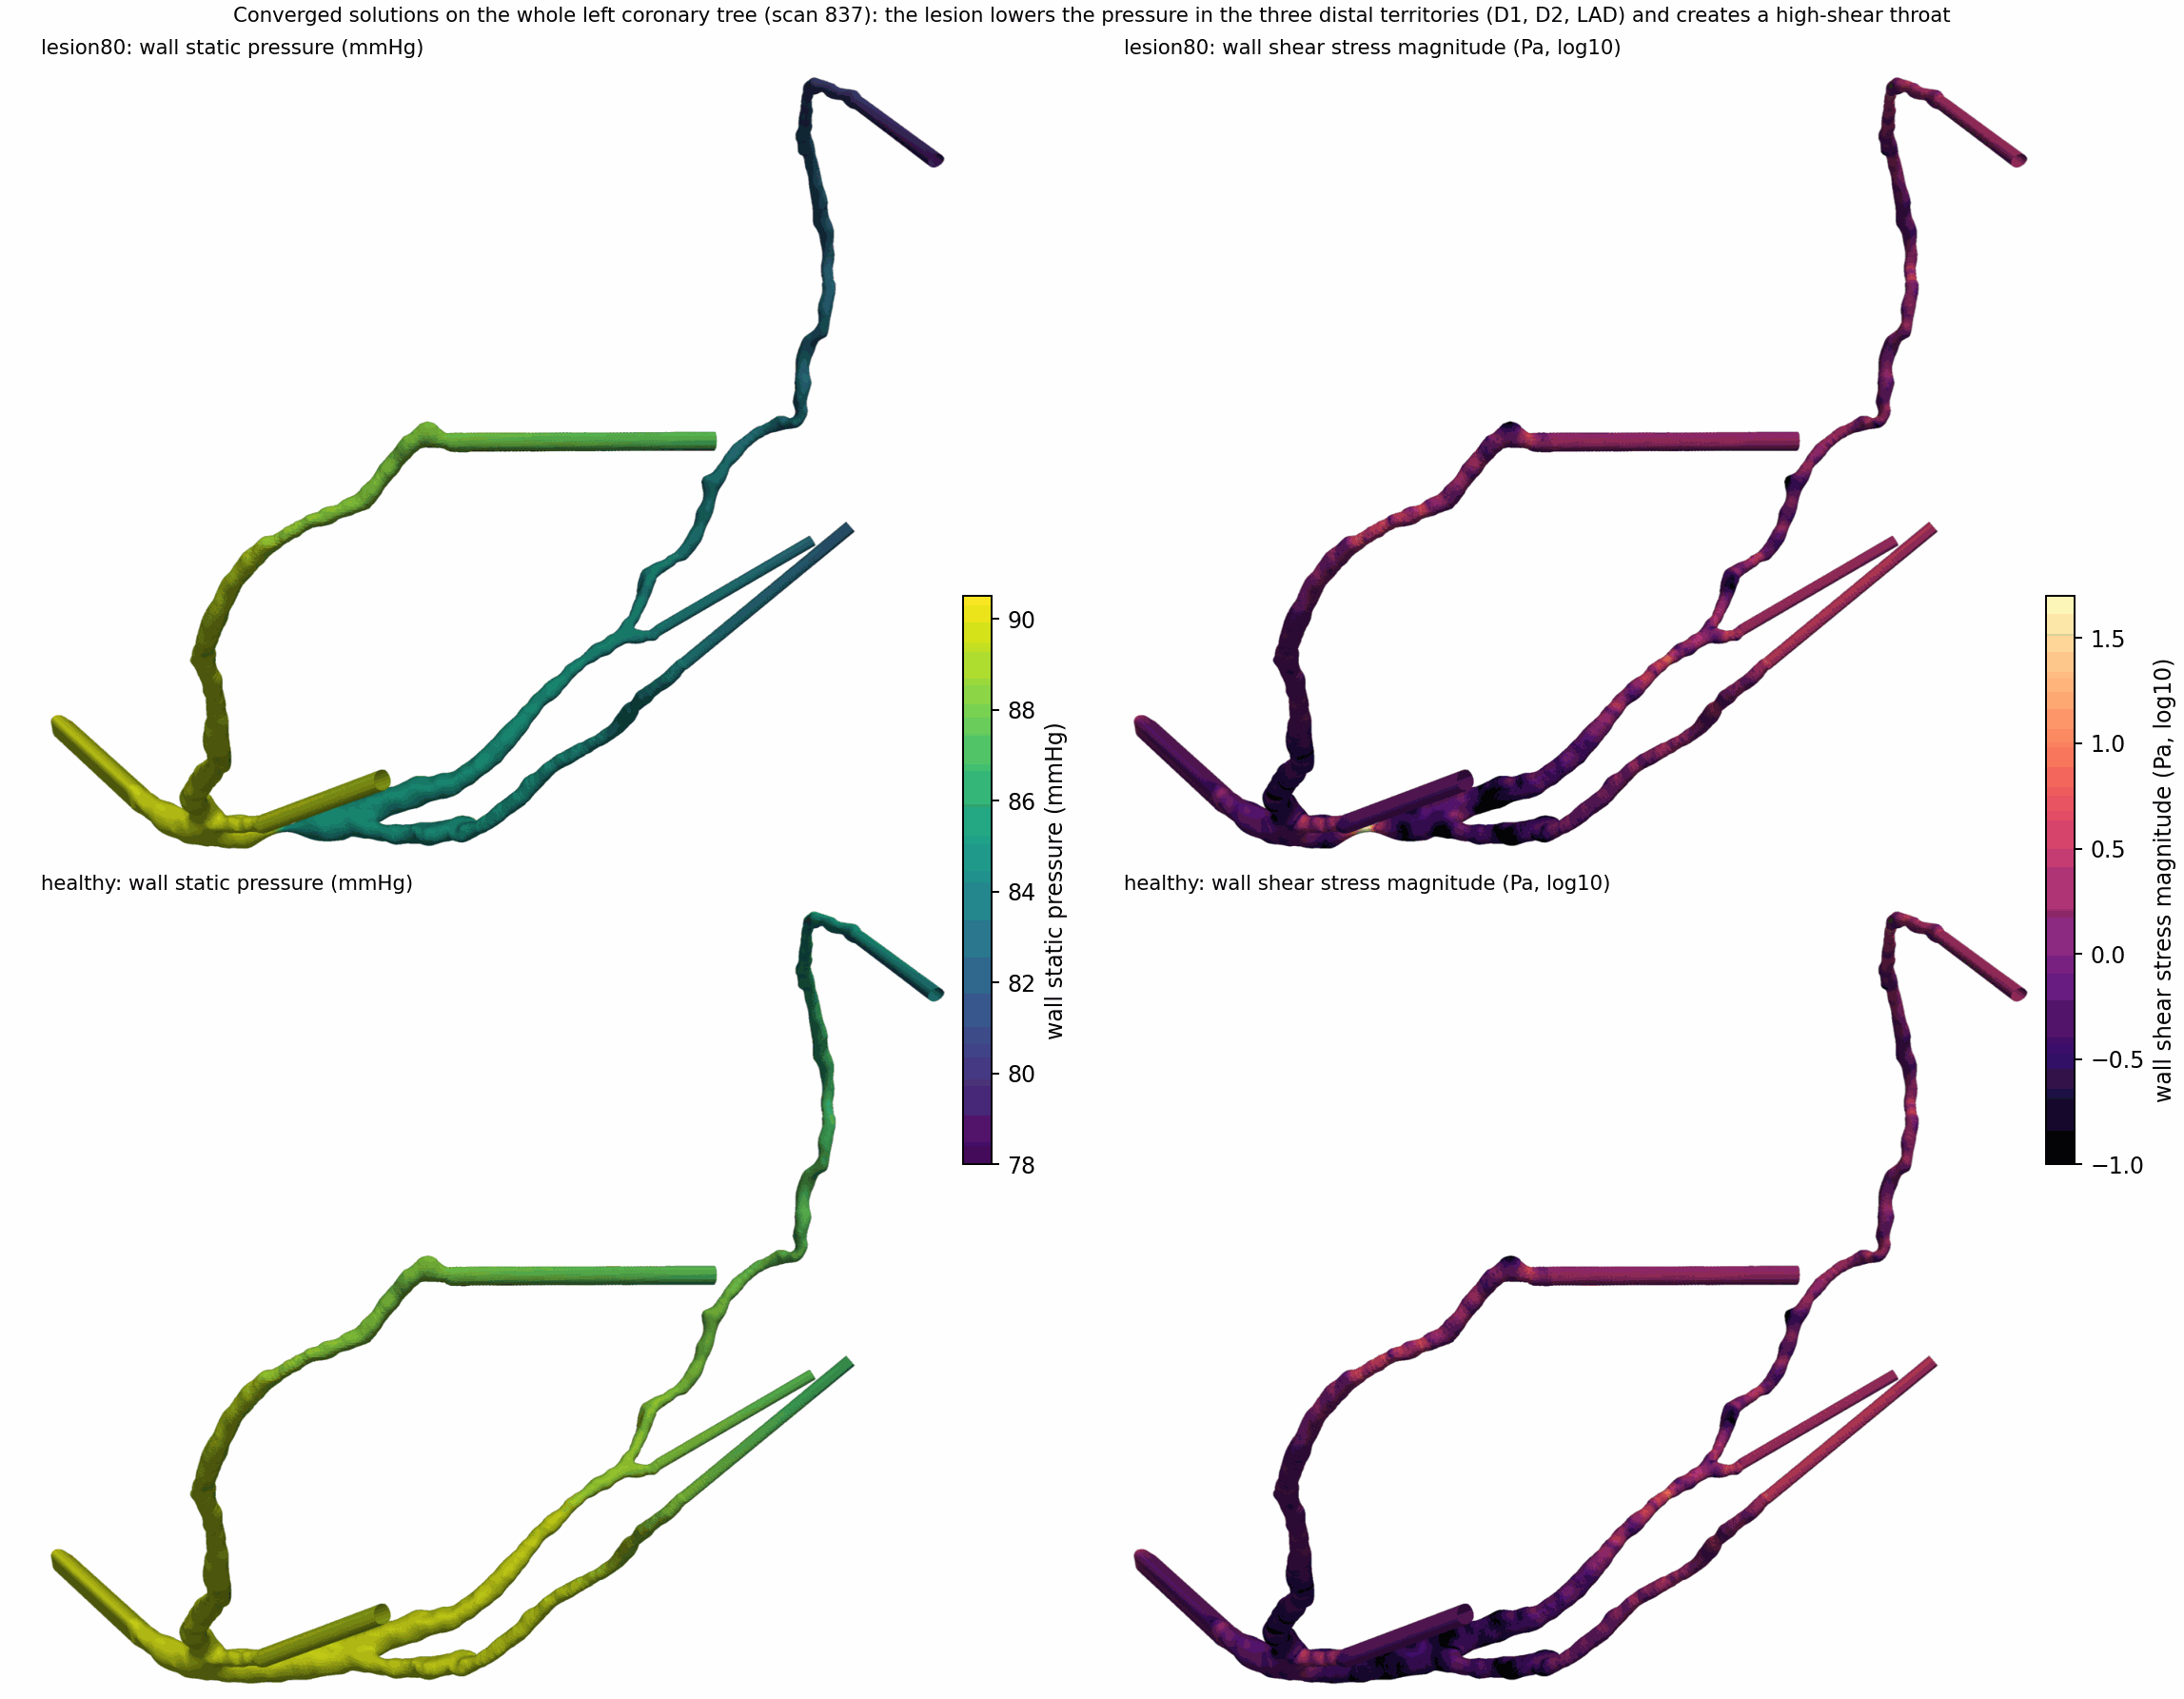
\includegraphics[width=\textwidth]{figures/cfd_tree_fields.png}
\caption{Wall static pressure (left) and wall shear stress magnitude (right) on the whole left coronary tree, lesion80 (top) and healthy reference (bottom), identical colour scales. The lesion lowers the pressure in the three territories distal to it (LAD, D1, D2; outlet pressure ratios 0.88--0.92 against 0.93--0.97) while LCX and IM are unchanged.}
\end{figure}

\paragraph{Mesh-sensitivity study of the lesion80 throat: design, pre-registered rules and audits (results follow below when the runs have finished).}
\label{sec:sens-design}
The lesion80 result above is a single-mesh result. Three further meshes of the \emph{same} surface, boundary conditions, numerics and 0D twin were built and run under the same audited launch procedure: \textbf{W100} (100\,$\mu$m cells in the whole refined tube, 1.30\,M cells), \textbf{T25a} (25\,$\mu$m for arc 20.5--26.5\,mm inside the 50\,$\mu$m tube, 3.53\,M cells) and \textbf{T25b}
(25\,$\mu$m for arc 19--28\,mm, 5.03\,M cells), against the audited \textbf{M50} (50\,$\mu$m, 2.68\,M cells; not re-run). Cell sizes are quantised by cfMesh to 0.2\,mm/$2^n$, so the levels differ by exactly a factor 2; the sizes were measured, not assumed (p95 of the cell size in the throat zone 103.9, 51.5, 25.6 and 25.6\,$\mu$m); the throat area of the mesh against the STL is
$-2.01$, $-0.33$, $-0.08$ and $-0.08\%$ respectively, and the boundary-layer stack (three layers, ratio 1.2) scales with the cell size (throat-station stack 75, 38, 20.5 and 20.5\,$\mu$m). Fig.~\ref{fig:mesh-levels} shows the four levels.
\textbf{Design changes made before any of these solves, and why.} A planned coarse throat-only level (T100) was rejected by its own gate (flagged cells inside the lesion tube at the size-jump interface); a first second fine mesh (zone 20.5--28\,mm) shared its upstream interface with T25a and could not test interface contamination, so T25b moves \emph{both}
interfaces (19 and 28\,mm against 20.5 and 26.5\,mm). A 25\,$\mu$m zone over the whole analysis window would need $\approx$9\,M+ cells and exceed the 27\,GB of RAM, so the fine side is a throat-zone refinement only; consequently the level set is \emph{not} a systematic refinement family and \textbf{no GCI, order of accuracy or uncertainty bound is computed}
(Item~2 had already shown a three-level GCI can be untrustworthy). The recirculation tail beyond the refined tube (which ends at arc 36\,mm; the recovery of the reversed flow at $\approx$38.5--39\,mm lies in 100--200\,$\mu$m cells in every level) is resolution-limited by construction whatever its label.
\textbf{Pre-registered rules (fixed before the solves; engineering judgement, not from the study specification; not changed after seeing any result).} Ten quantities: distal and total flow reduction against the healthy reference (tolerance 0.5 percentage points), the added static pressure loss between arc 18.5 and 29.5\,mm (3\%; the loss is taken at 29.5\,mm because there is no section at 30\,mm --- an earlier table of this report used the
29.5\,mm values under the label 30.0), the pressure minimum (0.3\,mmHg), peak velocity (5\%), peak throat wall shear (5\%), the onset arc (0.25\,mm) and recovery arc (1\,mm) of reversed wall shear, and the maximum reversed wall-shear fraction and reversed section-area fraction (0.05 each). A quantity is INSENSITIVE only if both 25\,$\mu$m levels stay within the tolerance of M50 and agree
with each other (so the interface positions cannot drive the result), with precedence UNASSESSABLE $>$ SENSITIVE $>$ INTERFACE-CONTAMINATED $>$ NON-MONOTONE $>$ INSENSITIVE; missing, invalid, non-finite, unconverged or time-inconsistent data give UNASSESSABLE and windows are never shrunk; outcome categories (separated or not, recovered or not) are compared before the numbers. INSENSITIVE is the only label that counts as a pass.
\textbf{Audits.} The three cases and the launch script were confirmed by Fable~5.1 and Gemini~3.8 Flash and, for the arithmetic, checked by all three auditors over eleven rounds: every round found genuine input-handling defects in the analysis script (a silent 30.0-versus-29.5\,mm station, missing-data windows, booleans read as numbers, duplicated or quoted headers, duplicate JSON keys,
NUL bytes, pandas accepting malformed quoting, an omitted output argument that silently analysed the default directories, and more); each was fixed and each fix tested (162 checks). Since the user's bug protocol of 2026-09-24 the fixes were made by Opus~5.5 (attempt 1 each) and only audited by the other models; before that date I fixed them myself, and Fable was called 13 times as an auditor (the user's rule is that the cap of two applies to bug fixes only; from 2026-09-24 the pre-run and post-hoc audits use Sonnet and Opus~5.5, with Gemini and Astra as further audit-only reviewers).
The analysis code was frozen with Gemini and Astra confirming the final version (round 11); after the runs, two further independent audits by Opus~5.5 and Sonnet (round 13) each re-derived all ten labels and every level value from the raw analysis, section and wall-shear files with their own code and found no difference (maximum relative difference $<10^{-6}$; the closest approach to a tolerance is the added static loss at 0.49 of its tolerance for the fine levels) and returned no blockers.

\begin{figure}[H]
\centering
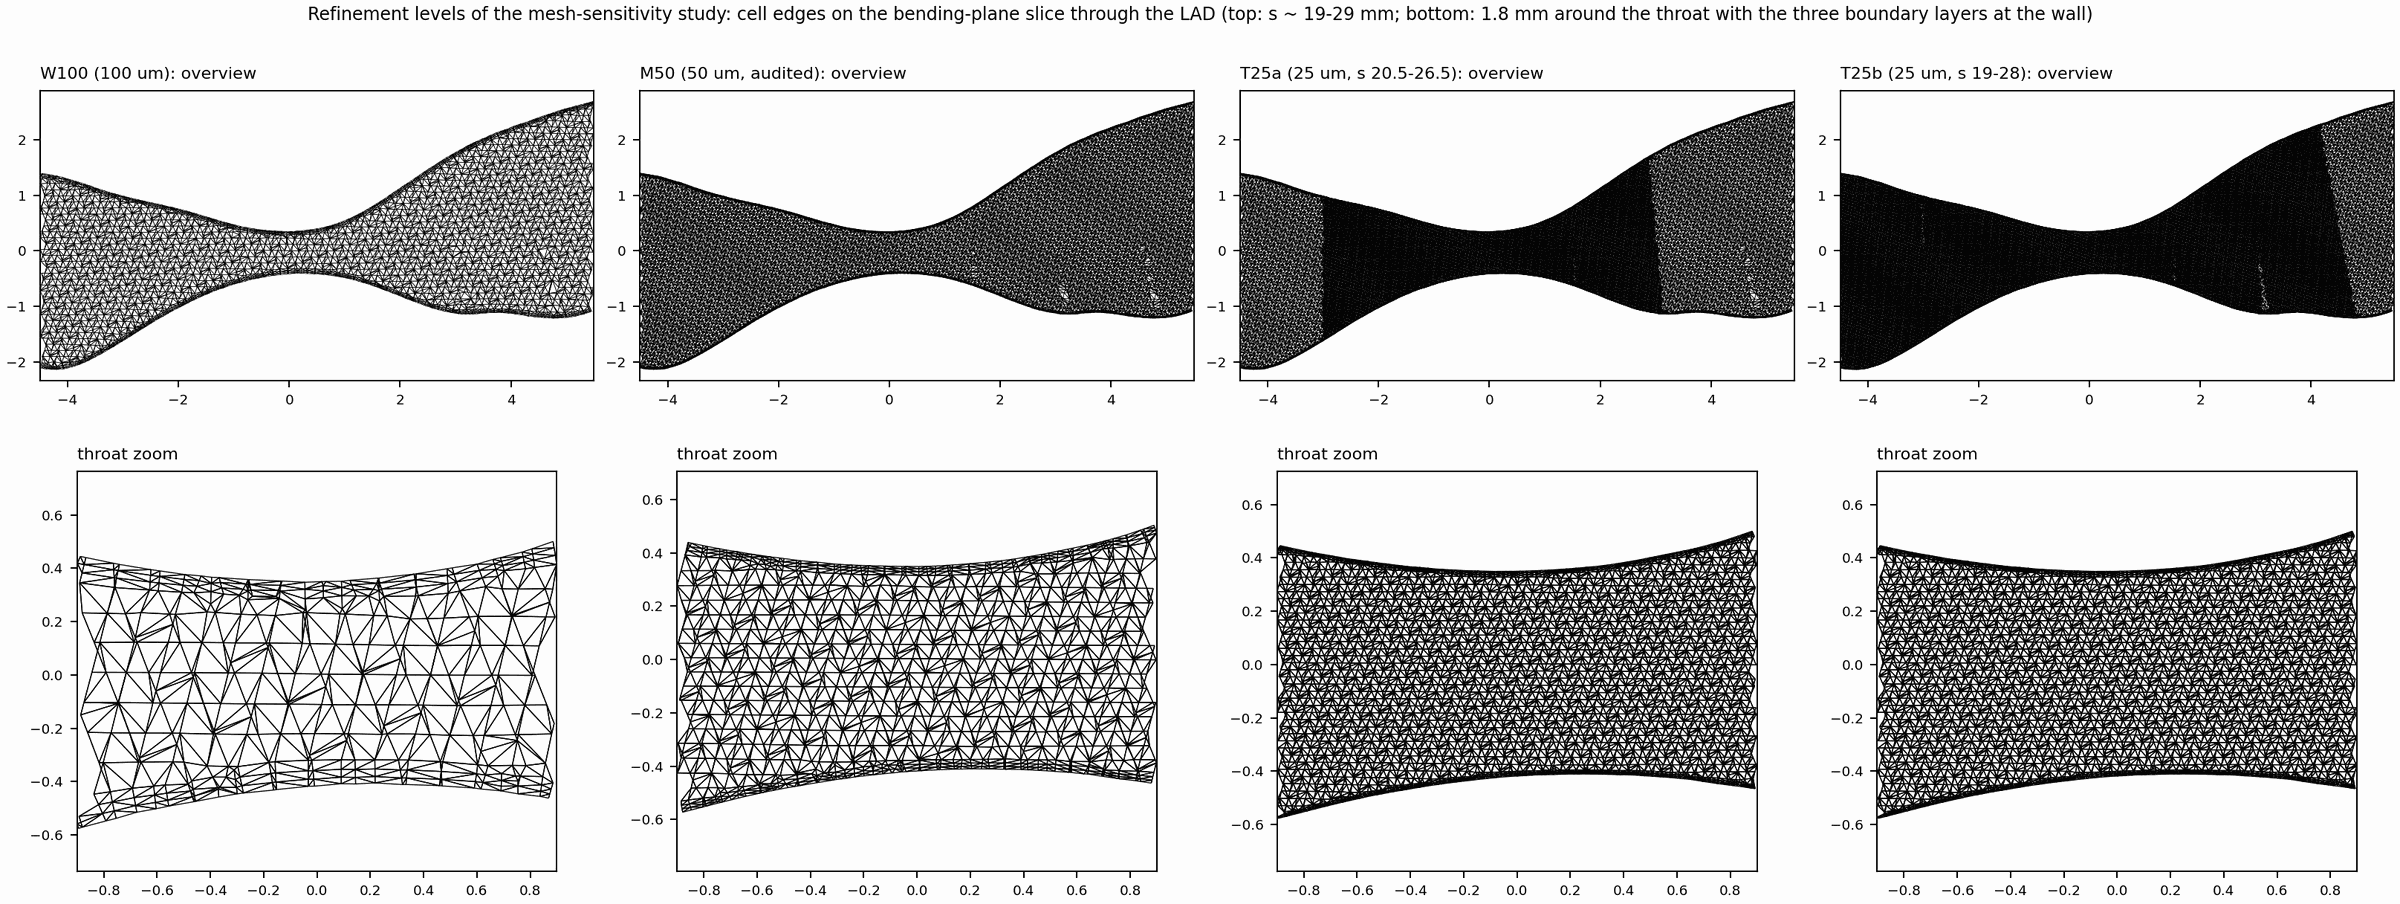
\includegraphics[width=\textwidth]{figures/cfd_mesh_levels.png}
\caption{\label{fig:mesh-levels}The four refinement levels on the bending-plane slice through the LAD (slice triangulation of the polyhedral cells): W100 (100\,$\mu$m), M50 (the audited 50\,$\mu$m mesh), T25a (25\,$\mu$m for arc 20.5--26.5\,mm) and T25b (25\,$\mu$m for arc 19--28\,mm); bottom row: 1.8\,mm around the throat with the wall-adjacent boundary layers. The refinement interfaces of the two T25 meshes (density changes in the top row) are at different arcs on both sides.}
\end{figure}

\paragraph{Mesh-sensitivity results: every pre-registered quantity is INSENSITIVE --- with the limits stated below.}
\label{sec:sens-results}
All three new runs converged under the predefined criteria (W100 in 688 iterations, T25a in 1315, T25b in 1470; final pressure residual $\leq2\times10^{-7}$, velocity residuals $\leq9\times10^{-6}$, every outlet flux stable to $\leq0.05\%$ over the last 200 iterations (W100 $\leq0.04\%$, T25a and T25b $\leq0.0012\%$), mass imbalance $\leq2\times10^{-6}\%$, BC-accuracy error $\leq5\times10^{-4}\%$; \textbf{convergence and BC accuracy: \PASS{}} for all three), and were stopped gracefully by the watcher.
The frozen analysis script (checksums recorded before any result was computed) then produced, from analysis, section and wall-shear files that share the reconstructed final iteration of every level:

\begin{table}[H]
\centering
\caption{\textbf{[PILOT\_OUT\_OF\_COHORT: scan 837]} Mesh-sensitivity of the lesion80 throat under the pre-registered rules. Flow reductions are relative to the healthy reference; the added static loss is $(P_{18.5}-P_{29.5})_\text{lesion}-(P_{18.5}-P_{29.5})_\text{reference}$. $^{\dagger}$Recovery lies outside the refined tube and is resolution-limited by construction (see text).}
\small
\setlength{\tabcolsep}{4pt}
\begin{tabular}{>{\raggedright\arraybackslash}p{7.0cm}rrrrrl}
\toprule
Quantity & W100 & M50 & T25a & T25b & Tol. & Label \\
\midrule
distal flow reduction (pp of reference) & 5.703 & 5.479 & 5.398 & 5.398 & 0.5 pp & INSENSITIVE \\
total flow reduction (pp) & 3.063 & 2.943 & 2.900 & 2.900 & 0.5 pp & INSENSITIVE \\
added static loss 18.5$\to$29.5\,mm (mmHg) & 4.931 & 4.741 & 4.671 & 4.671 & 3\% & INSENSITIVE \\
minimum static $P/P_\text{aorta}$ & 0.9335 & 0.9361 & 0.9368 & 0.9368 & 0.0033 & INSENSITIVE \\
peak axial velocity, arc 22--26 (m/s) & 1.200 & 1.160 & 1.148 & 1.148 & 5\% & INSENSITIVE \\
peak mean wall shear, arc 22--25 (Pa) & 57.87 & 54.74 & 53.60 & 53.60 & 5\% & INSENSITIVE \\
onset of reversed wall shear (arc, mm) & 24.25 & 24.25 & 24.25 & 24.25 & 0.25 mm & INSENSITIVE \\
recovery of reversed wall shear$^{\dagger}$ (arc, mm) & 39.00 & 39.00 & 39.00 & 39.00 & 1 mm & INSENSITIVE \\
max reversed-wall fraction, arc 24--39 & 0.942 & 1.000 & 1.000 & 1.000 & 0.05 & INSENSITIVE \\
max reversed section-area fraction, arc 24--38.5 & 0.667 & 0.670 & 0.671 & 0.671 & 0.05 & INSENSITIVE \\
\bottomrule
\end{tabular}
\end{table}

\textbf{What the numbers say.} Refining the throat zone from 50 to 25\,$\mu$m changes the distal flow reduction by $-0.08$ percentage points ($5.48\to5.40$), the added static loss by $-1.5\%$ ($-0.07$\,mmHg), the pressure minimum by $+0.0007\,P_\text{aorta}$ (0.06\,mmHg), the peak velocity by $-1.0\%$, the peak throat wall shear by $-2.1\%$ ($-1.1$\,Pa) and the maximum reversed-wall and reversed-area fractions by $\leq0.002$;
the onset and recovery arcs of reversed wall shear do not move. The two 25\,$\mu$m meshes, whose refinement interfaces are at different arcs on both sides, agree with each other to $2\times10^{-4}$ (flows and loss), $<10^{-3}$ (fractions) and $<10^{-3}$ relative (velocity and wall shear), so the interface position has no visible effect on any registered quantity.
Coarsening to 100\,$\mu$m moves the same quantities in the same direction by 2.3--3.7 times as much (loss $+4.0\%$, peak velocity $+3.5\%$, peak wall shear $+5.7\%$, distal flow reduction $+0.22$\,pp): the series W100, M50, T25a is monotone for every quantity and the change per halving shrinks, but the 100\,$\mu$m mesh differs from the audited one by more than the registered tolerance in three quantities (added loss $+0.19$\,mmHg against 0.14, peak wall shear $+3.1$\,Pa against 2.7, maximum reversed-wall fraction $-0.058$ against 0.05), so a mesh that coarse would not have been adequate for the throat quantities. Fig.~\ref{fig:sens-fields} shows the level-to-level differences directly: the axial-velocity profiles of M50, T25a and T25b lie on top of each other (W100 visibly blunts the throat plug and lowers the jet at 26.5\,mm), and the zero-velocity and 0.3\,m/s contours of all four levels almost coincide.

\begin{figure}[H]
\centering
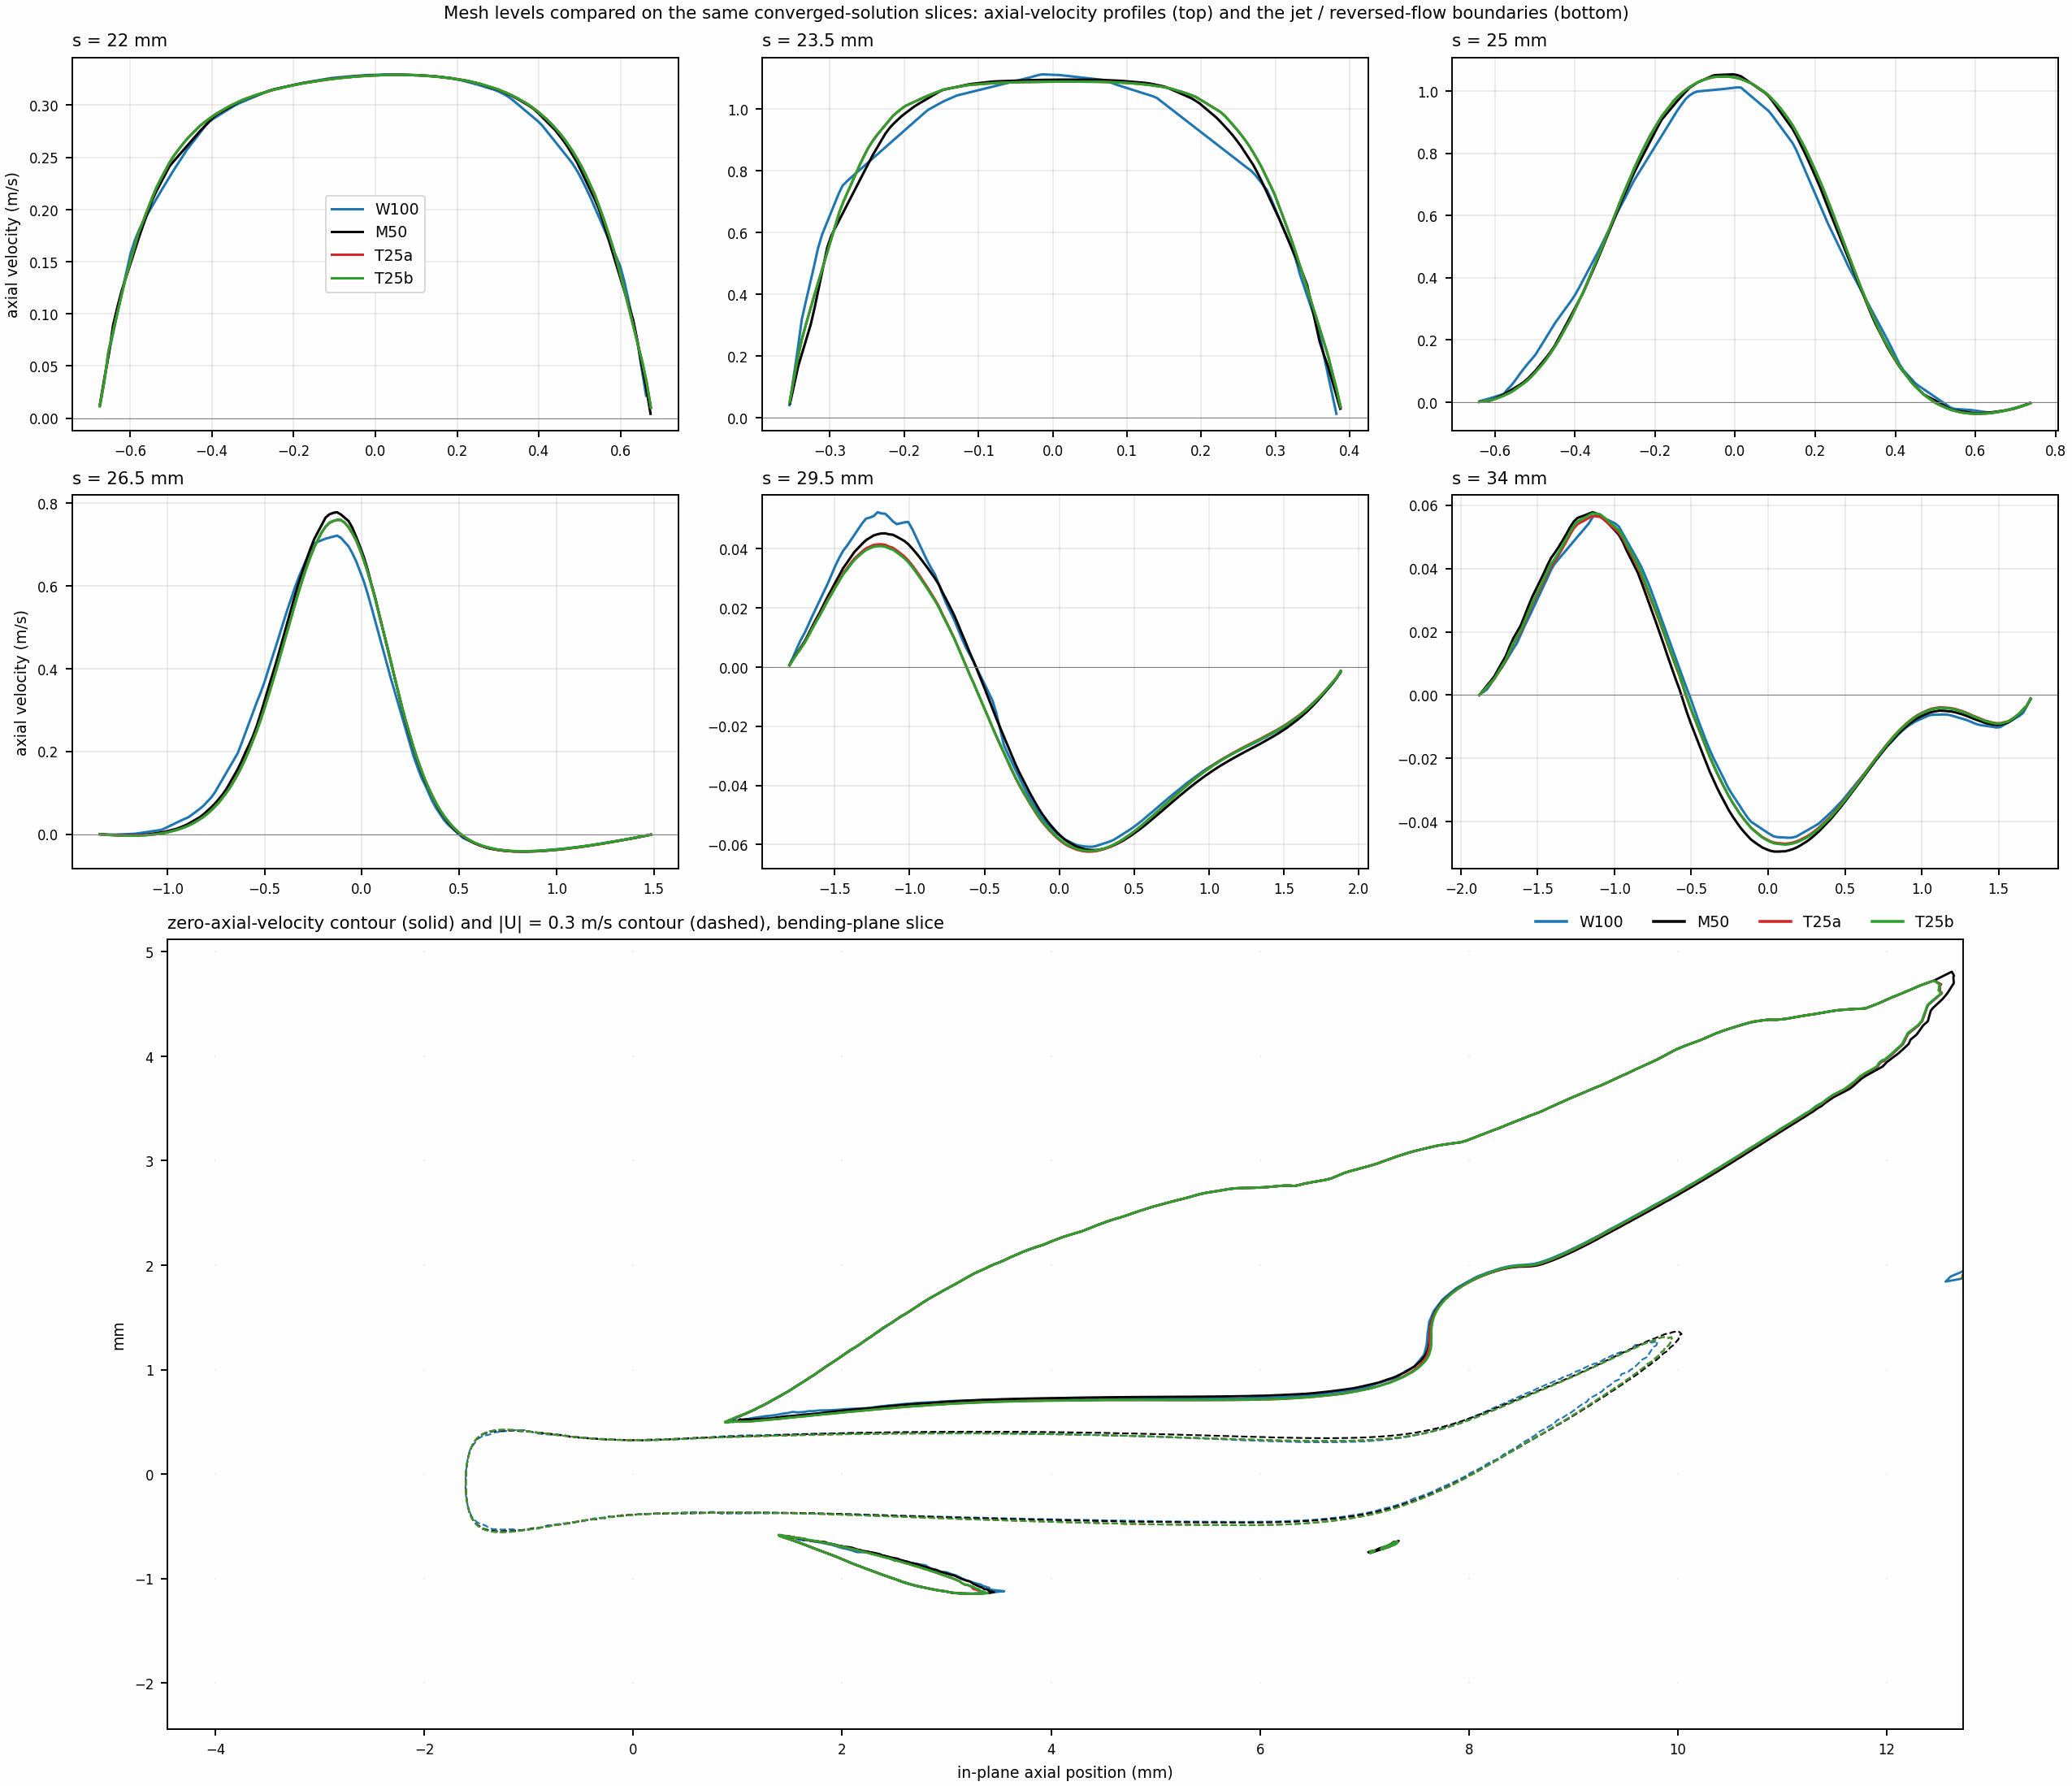
\includegraphics[width=\textwidth]{figures/cfd_sensitivity_fields.png}
\caption{\label{fig:sens-fields}The four mesh levels compared on identical slices of the converged solutions. Top: axial-velocity profiles across the lumen at six stations (W100 blue, M50 black, T25a red, T25b green; T25a is hidden under T25b). Bottom: zero-axial-velocity contour (solid) and $|U|=0.3$\,m/s contour (dashed) on the bending-plane slice, arc $\approx$21--36\,mm.}
\end{figure}

\textbf{Limits of this result (all stated in the design before the runs).} (i) INSENSITIVE means ``within the pre-registered tolerance for a factor-2 refinement'', not ``converged'': the tolerances are engineering judgement, no order of accuracy, GCI or uncertainty bound is computed (the level set is not a systematic refinement family), and a further halving is not tested. The lesion80 numbers of the preceding sections may therefore be read as mesh-dependent by roughly the amounts above
(order 1--2\% for the throat pressure loss and peak velocity, 2\% for the peak wall shear between 50 and 25\,$\mu$m), which is a description of what was observed, not a bound.
(ii) The onset arc (24.25\,mm) and recovery arc (39.0\,mm) are identical in all four levels, but the recovery lies in cells of 100--200\,$\mu$m outside the refined tube and is quantised to the 0.25\,mm station grid; agreement there shows the outcome is not sensitive to the throat-zone resolution, not that the recirculation extent is converged. The reversed-flow region itself was refined only up to 50\,$\mu$m in its core.
(iii) The fine side is a throat-zone refinement (25\,$\mu$m over 6--9\,mm of the $\approx$15\,mm long recirculating region); the effect of a finer expansion-zone mesh is not tested. (iv) The healthy reference was not re-run per level (its split moved $\leq0.01\%$ between 1.1\,M and 3.25\,M cells). (v) The STL facet size (0.017--0.24\,mm edges in the window) and the steady laminar assumption are untouched by this study.
(vi) One geometry, one flow, one patient. \textbf{Pass/fail:} all ten registered quantities are INSENSITIVE; that is the study's pass criterion, met, with the caveats above.
\textbf{Effect on the 0D--3D comparison:} the area-matched 0D twin's added loss (4.89\,mmHg) is $+3.1\%$ above M50 and $+4.7\%$ above T25a, and the EDT-radius 0D twin's (7.34\,mmHg) is $+57\%$ above T25a; the conclusion that the radius definition, not the loss law, dominates the difference is unchanged.

\textbf{Still open for Items 3 and 4.} A finer expansion-zone mesh and a further throat halving (the sensitivity study brackets the 50\,$\mu$m result but proves no convergence); the jet-reattachment length of an \emph{isolated} lesion (this geometry's lesion sits 8.5\,mm upstream of a
bifurcation, which the recirculation crosses); manual-repair minutes, which were not timed to the precision the design asks for; and a single end-to-end Item 4 runner. If the remeshing step is reinstated for future cases, its target edge length must be
constrained to $\lesssim r/3$ of the locally smallest vessel radius (here $\sim$0.2\,mm on 0.6\,mm branches) and gated by a pre-/post-remesh cross-section deviation check, not left at a single global value.

\subsection{Items 3 and 4, continued: hyperaemic flow, extended refined tube, isolated lesion, transient check, end-to-end runner}
\label{sec:followup}
This subsection reports the follow-up work commissioned after the mesh-sensitivity study (2026-09-24). Every new setup went through a read-only pre-run audit by GPT-6 Astra and Gemini~3.8 Flash before its solves started, every defect found (in the assistant's own scripts or by an auditor) was handed to Opus~5.5 (at most three attempts per defect set) and then Fable~5.1 (at most two), and finished runs received a post-hoc audit; the record is in \S\ref{sec:followup-audit}.

\paragraph{Hyperaemic flow: definition.} The study's 0D demand is $Q=k\,r_\text{in}^3$ with $k=562$\,s$^{-1}$ (the 0D code labels this demand ``hyperaemic'') applied to the 0D inlet radius, which is the mask-EDT radius (1.057\,mm) and is biased low: the 3D inlet patch of the two meshes has an area of 7.553\,mm$^2$ (radius 1.5505\,mm). The lower-flow pair of this report (called ``resting'' in tables and figures; the word labels the protocol demand of $0.6636$\,mL/s, not a measured resting state) used exactly that demand. The hyperaemic pair applies the same law to the 3D area-equivalent inlet radius: $Q_\text{hyp}=562\,(1.5505\,\text{mm})^3=2.0950$\,mL/s, $3.157\times$ the resting demand. No parameter was tuned, and the size of the ratio carries no physiological claim: it is a synthetic flow increase, not a measured flow reserve and not maximal hyperaemia. The bed constant of the 0D twin was recalibrated for $Q_\text{hyp}$ ($C$ from 246.94 to 73.17, all outlet resistances $\times0.2963$, relaxation factors 0.113/0.050/0.094/0.062/0.214 for LCX/IM/D1/D2/LAD). Meshes (the audited 2.68\,M-cell lesion mesh and 3.25\,M-cell healthy reference mesh), numerics, boundary-condition formulation and post-processing are the resting pair's; a file-level diff shows that only the outlet values, resistances and relaxation factors and a two-line comment differ. The outlet patches sit 20\,mm beyond the 0D leaves and their extension resistance is not compensated (about 6\% of $R_\text{out}$ at this flow, against 1.7\% at rest).

\paragraph{Hyperaemic flow: validity of the pair.} Both solves converged under the pre-registered strict rules (residuals $<10^{-5}$, mass imbalance $<10^{-6}\,\%$, boundary-condition error $\le0.0011\,\%$, flux and pressure bands $<0.1\,\%$ over 200 iterations, all monitors of equal length, logs finished): the healthy reference at iteration 1010 and the lesion case at 2106; the measurement-plane pressure ratio at four stations changed by at most $9\times10^{-6}$ (lesion) and $9\times10^{-5}$ (reference) between the final write and a write 356 and 260 iterations earlier (requirement $<10^{-3}$).

\begin{table}[H]
\centering
\caption{\textbf{[PILOT\_OUT\_OF\_COHORT: scan 837]} Hyperaemic pair against the resting pair (lesion80, same meshes). Flow changes are lesion minus healthy reference in the same flow state; ``0D EDT'' and ``0D area'' are the two 0D lesion variants.}
\label{tab:hyperaemia}
\small
\resizebox{\textwidth}{!}{\begin{tabular}{lrrrr}
\toprule
 & resting & hyperaemic & 0D EDT (hyp.) & 0D area (hyp.) \\
\midrule
total inflow, healthy reference (mL/s) & 0.6608 & 2.0248 & 2.0478 & 2.0478 \\
total flow change, 3D (\%) & $-2.94$ & $-11.93$ & $-17.03$ & $-13.04$ \\
D1 / D2 / LAD outlet change (\%) & $-5.5/-5.4/-5.5$ & $-23.6/-23.2/-22.8$ & $-33.1/-32.9/-32.9$ & $-25.4/-25.2/-25.2$ \\
throat flow (mL/s) / $Re$ (area-equiv.) & 0.338 / 151 & 0.807 / 362 & & \\
peak axial velocity, arc 22--26\,mm (m/s) & 1.16 & 2.46 & & \\
peak circumferential-mean wall shear, arc 22--25\,mm (Pa) & 54.7 & 180.0 & & \\
static loss added by the lesion, arc 18.5$\to$29.5\,mm (mmHg) & 4.74 & 20.64 & & \\
$p/P_\text{ao}$ at arc 40\,mm, lesion / healthy reference & 0.944 / 0.996 & 0.762 / 0.983 & 0.676 / 0.985 & 0.749 / 0.985 \\
\bottomrule
\end{tabular}}
\end{table}

\begin{figure}[H]
\centering
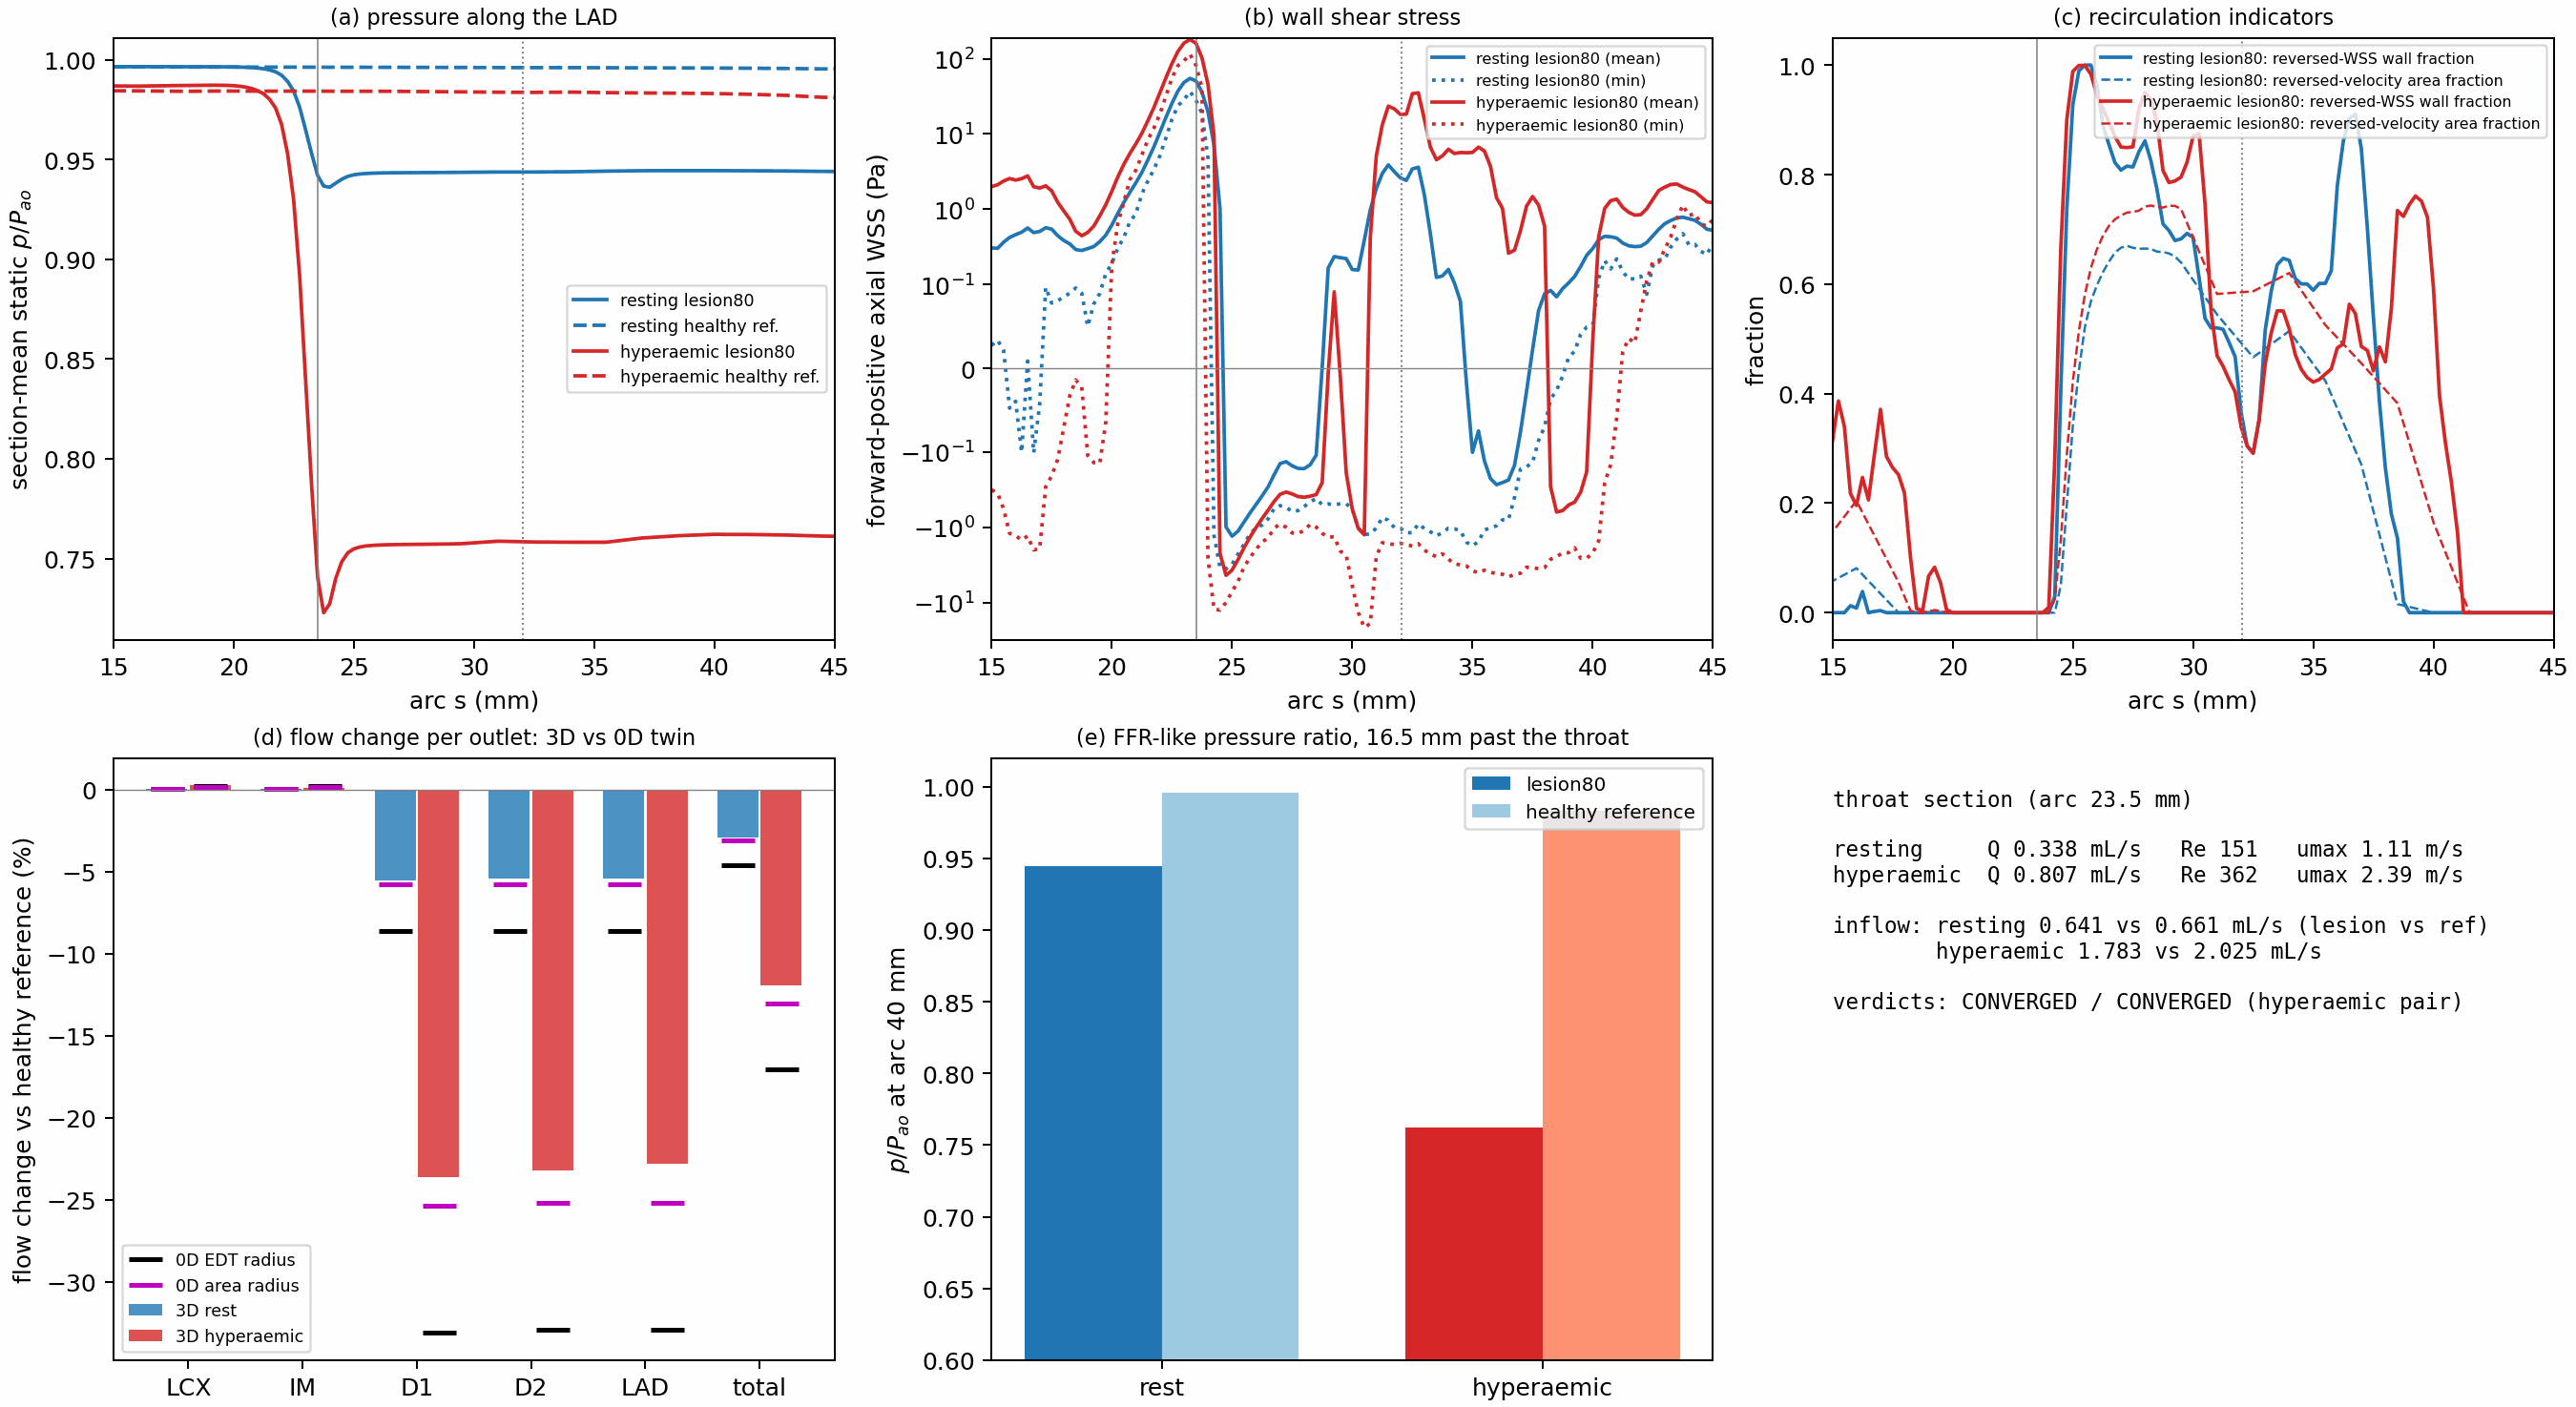
\includegraphics[width=\textwidth]{figures/cfd_hyperaemia.png}
\caption{\label{fig:hyperaemia}Resting (blue) and hyperaemic (red) lesion80 against their own healthy references. (a) Section-mean static pressure ratio along the LAD; (b) forward-positive axial wall shear (symmetric log axis); (c) reversed-wall-shear wall fraction and reversed-velocity section-area fraction; (d) outlet flow change against the two 0D variants; (e) pressure ratio 16.5\,mm past the throat. The reversed-flow extent in (c) beyond arc 34\,mm lies outside the 50\,$\mu$m refined tube (which ends at 36\,mm) and is diagnostic only.}
\end{figure}

\paragraph{Hyperaemic flow: results.} (i) \emph{Flow.} At $3.16\times$ the flow the lesion removes $11.9\,\%$ of the total inflow and about $23\,\%$ of the flow of the three distal outlets, against $2.9\,\%$ and $5.5\,\%$ at rest. The 3D change is smaller in magnitude than both 0D variants at every distal outlet and in total (pre-registered category (i), ``smaller than the area-matched 0D variant''), as it was at rest; the LCX outlet, whose change is only $+0.25\,\%$, falls in category (iii). This is a statement about ranking and sign, not agreement: the 3D distal reduction lies 1.7--2.4 percentage points below the area-matched variant and 9.5--10.2 below the EDT variant. (ii) \emph{Pressure.} The 3D static loss between arc 18.5 and 29.5\,mm rises from 4.74 to 20.64\,mmHg (a factor 4.35 for a throat-flow factor 2.39). The 0D variants bracket the loss up to the throat (22.2\,mmHg in 3D against 25.0 for the EDT variant and 19.1 for the area variant) but disagree qualitatively downstream of it: the 3D solution recovers 1.6\,mmHg of pressure between the throat and arc 29.5\,mm while both 0D variants keep losing (2.3--3.0\,mmHg). The pressure ratio at arc 40\,mm, a static, area-averaged FFR-like quantity relative to the 90\,mmHg inlet total pressure, is 0.762 in 3D against 0.749 (area variant) and 0.676 (EDT variant); the healthy reference gives 0.983. No clinical threshold is claimed. (iii) \emph{Loss law.} Solving $\Delta P=aQ+bQ^2$ exactly from the two flow levels (throat flows 0.338 and 0.807\,mL/s) gives $a=7.7\times10^8$\,Pa\,s\,m$^{-3}$ and $b=3.3\times10^{15}$\,Pa\,s$^2$\,m$^{-6}$, so the quadratic term carries 78\,\% of the loss at the hyperaemic flow; $\Delta P/Q^2$ falls from $5.5\times10^{15}$ to $4.2\times10^{15}$. The 0D expansion coefficient of the lesion window is $5.7\times10^{15}$\,Pa\,s$^2$\,m$^{-6}$ (all four 0D loss nodes together, including three native narrowings, $6.4\times10^{15}$). Two points solve the two coefficients exactly and therefore do not test the quadratic form; the comparison is descriptive. (iv) \emph{Jet and wall shear.} Peak axial velocity doubles (1.16 to 2.46\,m/s) and the peak circumferential-mean wall shear rises from 54.7 to 180\,Pa; separation still starts at arc 24.25\,mm; the reversed-flow region reaches 41\,mm in wall shear (38.75\,mm at rest) and 40\,mm in reversed-velocity area (38.5 at rest), and the reattachment outcome is again censored by the D1 ostium at arc 32.05\,mm.

\paragraph{Hyperaemic flow: what is and is not a finding.} The recirculation extent beyond arc 34\,mm is \textbf{not mesh-supported}: the 50\,$\mu$m tube ends at 36\,mm, so the tail lies in 100--200\,$\mu$m cells; the extents above (41 and 40\,mm) are diagnostic values and are not presented as results; the pre-registered flag (last reversed station more than 2\,mm inside the tube end) reads ``NOT MESH-SUPPORTED''. The flow, pressure, peak-velocity and peak-shear results above are not affected by this flag, but no hyperaemic mesh-sensitivity study was made (boundary layers thin with $Re^{-1/2}$, so the resting sensitivity study does not transfer). Further caveats: the healthy hyperaemic reference delivers 2.025\,mL/s, 1.1\,\% below the 0D twin and 3.4\,\% below the demand, with per-outlet deviations from the 0D split between $-6.1\,\%$ (D1) and $+5.6\,\%$ (LAD) against at most $+3.1\,\%$ at rest (the cause was not isolated); the demand is synthetic (no autoregulation, uniform resistance scaling); the solves are steady and laminar at a throat $Re$ of 362, which could hide unsteadiness (the transient check of this subsection covers only the resting case); the lesion is synthetic and the geometry single.

\paragraph{Extended refined tube (resting flow): the 36\,mm tube end does not move the ten registered quantities.} The refined 50\,$\mu$m tube of the resting pair ends at arc 36\,mm. To test whether this truncation affects the results, both resting cases were rebuilt with the refined tube extended (requested end 60\,mm; realised: the last 50\,$\mu$m cylinder ends at 58.0\,mm, the frame sequence at 58.83\,mm), meshed with the same recipe (lesion case 3.87\,M cells, healthy reference 4.43\,M), and solved with the same boundary conditions, numerics and 0D-derived resistances as the audited pair (16 ranks each, run concurrently). Both converged under the strict rules (lesion at iteration 1450, reference at 728; residuals $<10^{-5}$, boundary-condition error $<10^{-3}\,\%$, all bands $<0.1\,\%$); the measurement-plane pressure ratio at four stations changed by at most $1.2\times10^{-5}$ (lesion, over 450 iterations) and $5.8\times10^{-4}$ (reference, over 478 iterations; the earlier write of the reference case is at iteration 250 because the case converged early, so this change is the least stringent of the four cases but below the $10^{-3}$ requirement). Table~\ref{tab:e60} gives the ten quantities of the frozen mesh-sensitivity analysis for the original (M50) and extended (E60) tubes, each pair against its own healthy reference.

\begin{table}[H]
\centering
\caption{\textbf{[PILOT\_OUT\_OF\_COHORT: scan 837]} Extended refined tube (E60) against the audited resting pair (M50). The tolerance is the frozen sensitivity tolerance of the ten quantities; no quantity moved.}
\label{tab:e60}
\small
\begin{tabular}{lrrrr}
\toprule
quantity & M50 & E60 & difference & tolerance \\
\midrule
distal flow reduction (\%) & 5.4788 & 5.4794 & $+0.0006$ & 0.5 \\
total flow reduction (\%) & 2.9430 & 2.9434 & $+0.0004$ & 0.5 \\
added static loss (mmHg) & 4.7410 & 4.7416 & $+0.0006$ & 0.142 \\
minimum $p/P_\text{ao}$ & 0.93610 & 0.93609 & $-0.00001$ & 0.0033 \\
peak axial velocity (m/s) & 1.16027 & 1.16035 & $+0.00009$ & 0.058 \\
peak throat wall shear (Pa) & 54.740 & 54.746 & $+0.006$ & 2.74 \\
separation onset, arc (mm) & 24.25 & 24.25 & 0 & 0.25 \\
wall-shear recovery, arc (mm) & 39.0 & 39.0 & 0 & 1.0 \\
max reversed wall fraction & 1.000 & 1.000 & 0 & 0.05 \\
max reversed area fraction & 0.6699 & 0.6703 & $+0.0004$ & 0.05 \\
\bottomrule
\end{tabular}
\end{table}

Every difference is below $0.8\,\%$ of its tolerance (largest: the maximum reversed area fraction, $0.72\,\%$ of its tolerance and $0.054\,\%$ of its value). The last reversed station lies at arc 38.5\,mm in both tubes (sections and wall), inside both analysed windows (49\,mm sections, 45\,mm wall); the pressure ratio at arc 40\,mm is $0.9444$ (lesion) and $0.9958$ (reference) for both tubes. The result therefore supports that the resting sensitivity study and the resting lesion80 results were not affected by the truncation at 36\,mm; it says nothing about the hyperaemic pair, whose reversed-flow tail ($40$--$41$\,mm) extends beyond the tube end and which was not repeated on the extended tube (the follow-up work order closed new work on this geometry). The hyperaemic extent quantities therefore remain diagnostic and NOT MESH-SUPPORTED, as stated above. Limits: one geometry and one flow; wall-clock figures of this pair are contended (32 ranks on 16 physical cores until iteration 728 of the lesion case; see the timing table of the returned data).

\paragraph{Audit and defect-handling record.}\label{sec:followup-audit} \emph{Roles} (set by the study lead on 2026-09-24): the main assistant does the work; GPT-6 Astra and Gemini~3.8 Flash audit only, before a setup runs and after it has finished, read-only; a defect of any kind (also in the assistant's own scripts) goes to Opus~5.5 (at most three attempts), then Fable~5.1 (at most two), then stops and is reported; the fixes are verified by the assistant and audited again. \emph{Follow-up tooling of this subsection} (hyperaemic pair, extended tube, isolated-lesion and transient setups, end-to-end runner): six audit rounds by both auditors; reporting and launch tooling needed Opus attempts 1--3 and Fable attempts 1--2 (Fable's first attempt ended before delivering a report; its second passed 59 of 59 checks); the comparison scripts needed Opus attempts 1--2, the runner Opus attempts 1--2, the transient tooling Opus attempt 1. One auditor finding survived the attempt cap (a helper that could report ``end of the reversed region established'' when every downstream station was missing) and is disputed between the auditors; it was mitigated by reading the coverage counts of every analysis by hand. The isolated-lesion, transient and hyperaemic-on-extended-tube setups were built and audited but not run. \emph{Task-1 setup ($U_{3D}$)}: two audit rounds by Gemini alone (both READY WITH CONDITIONS) because GPT-6 Astra reached its usage limit until 2026-09-26 18:22 and the study lead decided on 2026-09-24 to proceed on one auditor; every finding was fixed (an outlet-flux sign, a binary-write setting, missing-file handling, two decision rules that contradicted the work order, a premature PASS wording without the shifted-zone family; Opus attempts 1 for each group), the launcher was generalised (coded-BC libraries derived from the case, rank cap 16, coded-free option, per-case iteration budgets: 221 asserting tests; Opus attempt~1 ended before finishing its test run, attempt~2 showed that the five failing checks were errors of the tests, not of the launcher). GPT-6 Astra's post-hoc audit of the $U_{3D}$ study (2026-09-26) is sound with caveats (two major findings on the wording of the wedge agreement and of the boundary-layer scaling, four minor ones on the provenance of budgets and thresholds, settled-onset iterations, the diagonal minimum of the cell count and missing analysis safeguards); the reporting findings are incorporated in \S\ref{sec:u3d}, the code findings were handled by the defect protocol; its post-hoc audit of the Task-0 returns found no numerical error (every sampled number reproduced) but reported defects that were corrected: the scan-837 label \texttt{PILOT\_OUT\_OF\_COHORT} missing in the failures table, its notes and the captions of eight scan-837 tables of this report; two files missing from the code deposit (the pullback generator and the frozen sensitivity design); a printout that called the segmented-network minimum FFR \texttt{healthy\_main\_ffr} (Opus attempt~1); stale statements of the returned notes and of this abstract; and the incomplete case template (a complete case as run was added); its post-hoc audit of Task 3 found the completed round trips numerically sound (it recomputed every Item-1 and baseline flow, pressure, derived resistance and error) and reported: Gate M1 remains unpassed (the literal throat check and the self-intersection gate fail), the localisation of the mesh failures had been overstated (corrected in \S\ref{sec:m1}), the explanation of the flow split overstated the exclusion of set-up errors (reworded), two residual and error figures were imprecise (corrected), the day accounting needed a working-day ledger (added), and the queue and cached-analysis safeguards did not enforce scientific verdicts (a corrected queue and analysis scripts are with the defect protocol, Opus attempt~1; the finished cases were unaffected: its independent check reproduced their cached numbers). Its audit of the Task-4 timing tooling (verdict NOT READY) found that OpenFOAM's \texttt{ExecutionTime} is CPU time (the wall figure must come from \texttt{ClockTime}), that isolation on a WSL2 host cannot be certified by Linux guards alone, and missing validity gates and clean-up; these went to Opus attempt~2 and the timing run has not been made. \emph{Task-3 setups} (prescribed-flow round trip, scan-14 geometry, meshes and cases): one Gemini round each, READY WITH CONDITIONS, no code defect. \emph{Post-hoc audit of the returned data} (Gemini): sound with caveats; every sampled number was reproduced from the raw monitors. \emph{The assistant's own errors, found by data re-audits and corrected in place in this report:} the Item~6 timing was called isolated but was not; the sten70 level-4 solution was called converged although its monitor kept drifting and its residuals were high; the A4 round-trip error and the A3 sten50 run were described from an intermediate plateau and as stopped early; the gate of the scan-828/837 selection was misnamed; the count ``8 of 8'' could not be reproduced (the running summary has seven pass/fail rows). \emph{Mechanical incidents, not defects:} the CLI binaries were briefly unavailable during an automatic update, the Gemini service failed several times with transient DNS or eligibility errors (retried), and a root-disk shortfall (below the launcher's 10\,GB floor) was resolved by moving finished cases to another drive.

\subsection{Task 1 of the 2026-09-24 work order: the 3D discretisation uncertainty $U_{3D}$ of sten70}
\label{sec:u3d}
\textbf{Question.} \S\ref{sec:item2} left the 3D FFR discretisation uncertainty of sten70 undefined: the four-level ladder was not a systematic refinement family (settings held while the realised boundary-layer stack and the core cell size varied), and its finest level was not converged. The study's statistics plan has a pre-registered rule waiting on this number. \textbf{Design.} The classification, the thresholds (0.005, the noise factor 0.25) and the choice of the Celik--Eça--Hoekstra index were written in the design document (versions 2.1 and 2.2) and audited before any solve; the SETTLED criterion (version 2.4) was fixed after the first wedge run had shown a drifting finest level but before the first 3D result (the code carries a file time 3\,min after the S50 launch and 1\,h 43\,min before its result). The iteration budgets of S25A, S25B, S12A and S12B (versions 2.5--2.7) and the reduction of the S12B budget were set \emph{with earlier results in view}, on settling behaviour only, never on FFR values; this is disclosed adaptation, not a wholly prospective registration, and file times cannot prove that live results were unseen. The post-hoc audit found no evidence that $U_{3D}$ was steered: with 3000 iterations for every 3D level the result would be 0.0005477, i.e.\ $3.6\times10^{-9}$ below the reported value. Straight tapered vessel of Stage A, 70\% diameter stenosis (throat diameter 0.891\,mm), one outlet with the coded resistance $R=6.974826\times10^9$\,Pa\,s\,m$^{-3}$, relax 0.20, inlet total pressure 90\,mmHg, steady laminar \texttt{simpleFoam}, the audited numerics of Stage A, a fixed iteration budget fixed per level in advance (no residual-based stopping). A finer surface (192 circumferential facets, 20\,$\mu$m axial rings in the lesion) replaced the Stage A STL. Three 3D levels with throat-zone cell sizes of 50, 25 and 12.5\,$\mu$m (cfMesh sizes are $0.2\,\text{mm}/2^n$, so the ratio is exactly 2), four boundary layers of ratio 1.2 whose stack scales with the local cell size, the same lesion zone (11.5--51.5\,mm) at 50\,$\mu$m for every level, the throat zone A (29--34\,mm) at 25 or 12.5\,$\mu$m, and, for the interface-contamination test the work order requires when only a throat zone is refined, a second throat zone B shifted by 1\,mm at both ends. A 2D axisymmetric wedge family (blockMesh, 2$^\circ$, four levels of ratio 2 in every direction, the same boundary conditions with the wedge-scaled resistance) serves as the physics-versus-discretisation cross-check. The pre-registered rules: the FFR of a level is the last-100-iteration mean of the area-averaged pressure at $x=56.5$\,mm over the aortic pressure; a level is analysed only if it is \emph{settled} (drift over the final 500 iterations $\leq2\times10^{-4}$ and last-100 band $\leq10^{-4}$); rule~1 (the differences shrink in every family, no family is noise-limited and every finest pair is $<0.005$) gives $U_{3D}$ as the larger Celik--Eça--Hoekstra GCI$_{21}=1.25\,|e_{21}|/(2^p-1)$ of the families; rules~2 and~3 handle flat families with the wedge and the transient fallback; without both families the outcome is only provisional.

\begin{table}[H]
\centering
\caption{$U_{3D}$ ladder of the 3D family (measured meshes; every solve on 16 ranks, one at a time; the memory column is the sum over the simpleFoam processes on the host).}
\label{tab:u3d-levels}
\small
\resizebox{\textwidth}{!}{\begin{tabular}{lrrrrrrrr}
\toprule
level & cells & cells across throat (median/min) & p95 cell ($\mu$m) & BL first/stack ($\mu$m) & iterations & FFR & wall (h) & RAM (GB) \\
\midrule
S50 & 2{,}687{,}640 & 26.5 / 20 & 51.2 & 7.1 / 39.0 & 3000 & 0.793362 & 1.8 & 4.7 \\
S25A & 3{,}194{,}196 & 47.5 / 33 & 25.5 & 3.9 / 21.6 & 4000 & 0.791103 & 2.6 & 5.3 \\
S12A & 6{,}739{,}168 & 88.0 / 58 & 12.7 & 1.5 / 8.6 & 6000 & 0.790308 & 8.2 & 9.8 \\
S25B & 3{,}299{,}948 & 47.5 / 33 & 25.6 & 3.9 / 21.6 & 4000 & 0.791197 & 2.9 & 5.4 \\
S12B & 7{,}649{,}800 & 88.0 / 58 & 12.7 & 1.5 / 8.6 & 3000 & 0.790418 & 5.7 & 10.9 \\
\bottomrule
\end{tabular}}
\end{table}

\begin{figure}[H]
\centering
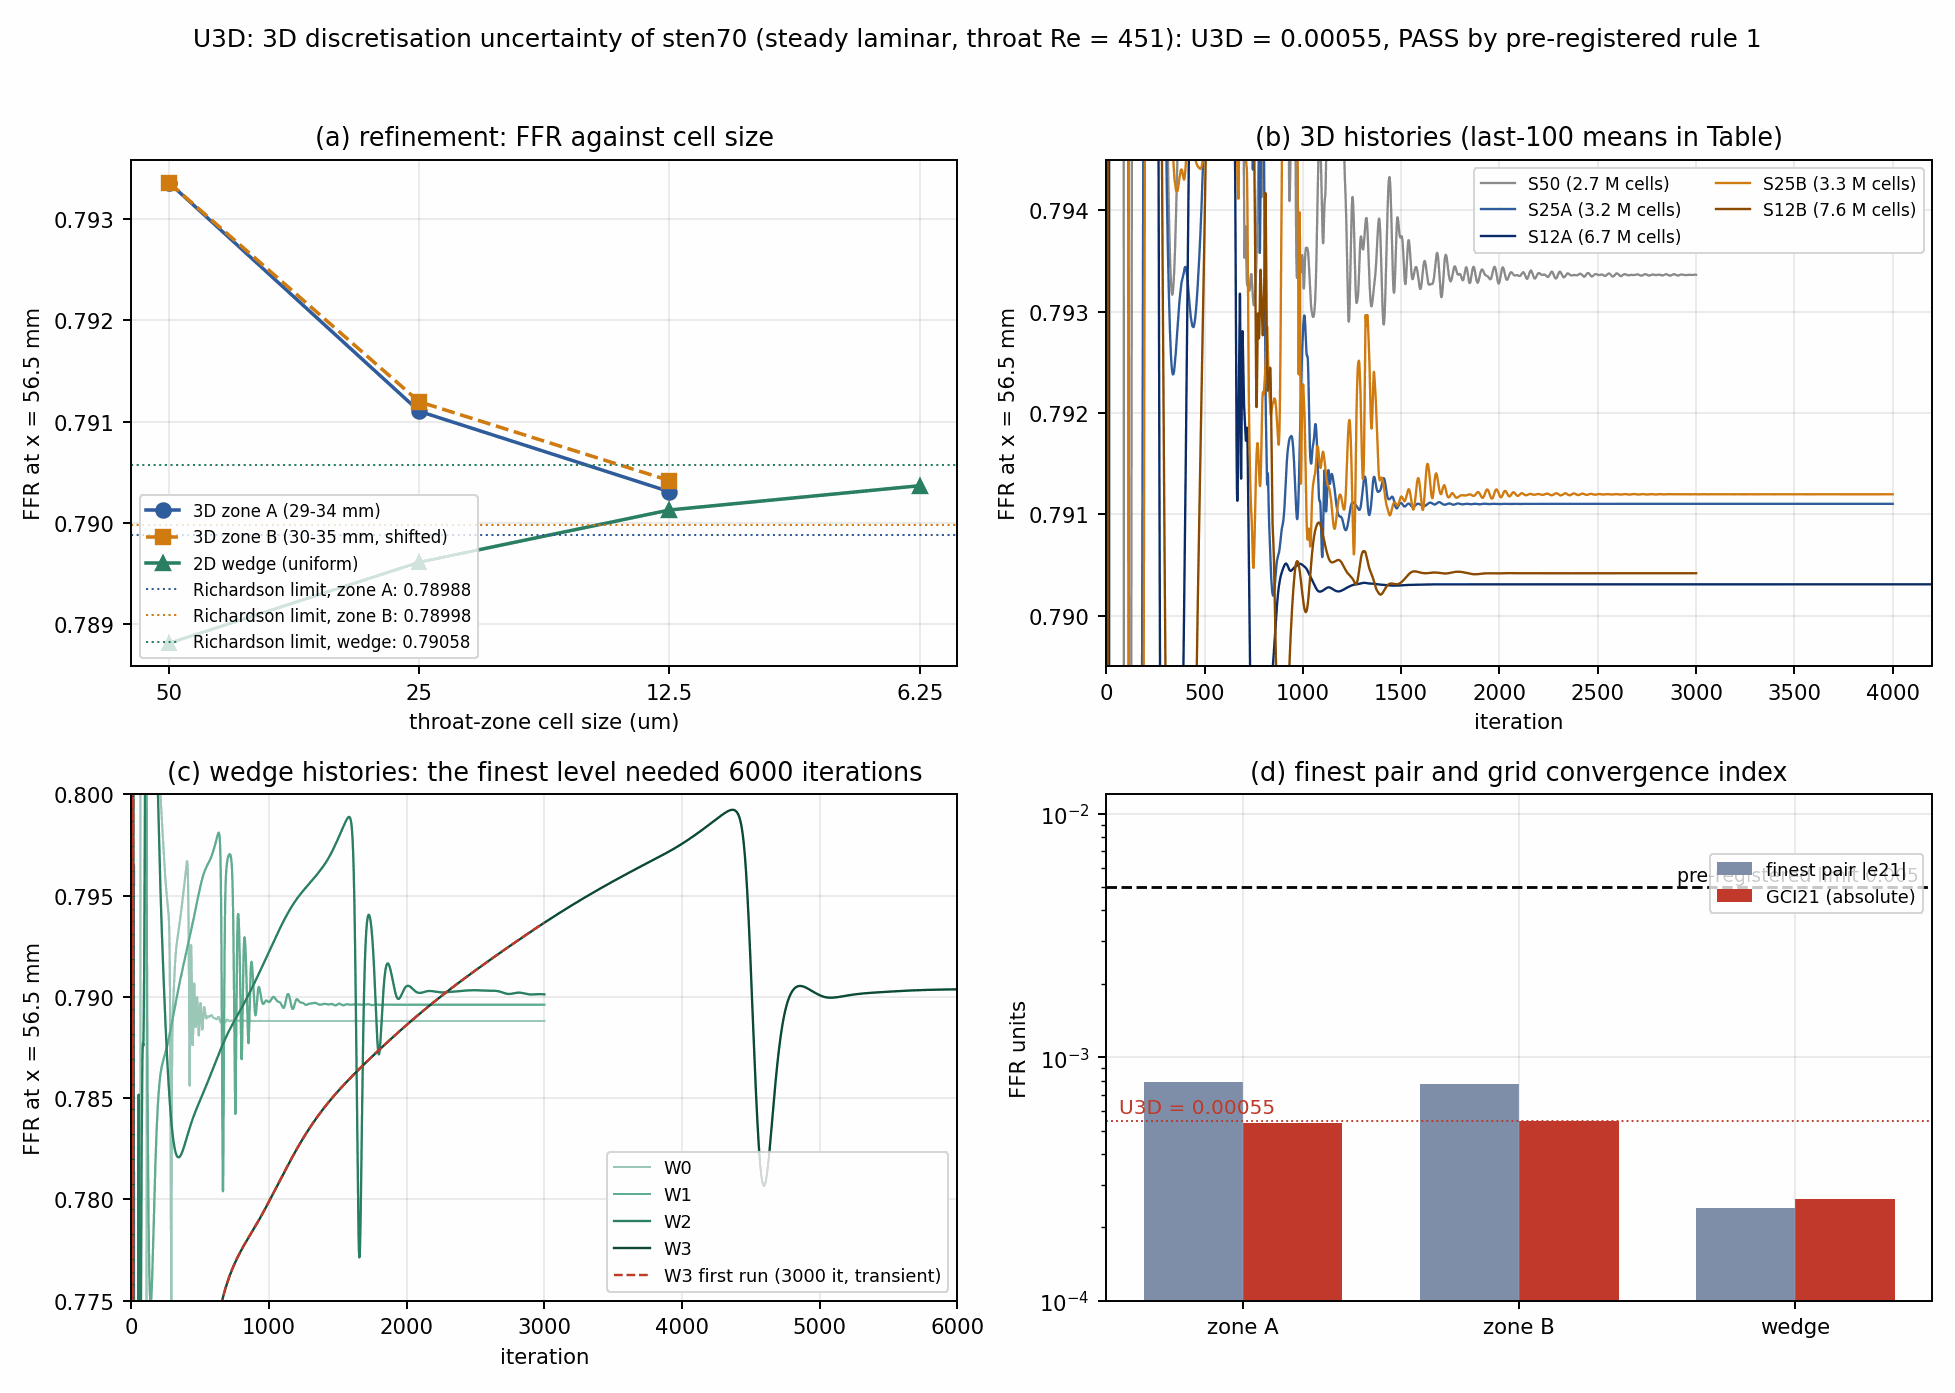
\includegraphics[width=\textwidth]{figures/cfd_u3d_convergence.png}
\caption{\label{fig:u3d}$U_{3D}$ study. (a) FFR at $x=56.5$\,mm against the throat-zone cell size for the 3D zones A and B and the 2D wedge, with the Richardson limits of the three families (the 3D families approach from above, the wedge from below). (b) Iteration histories of the five 3D levels (the last-100-iteration means are in the table). (c) Histories of the four wedge levels; the first 3000-iteration run of the finest level (red) was still drifting and was re-run with 6000 iterations. (d) Finest pair and grid convergence index of the three families against the pre-registered limit 0.005.}
\end{figure}

\textbf{Meshes and solves.} All five meshes passed the gates that were measured on the mesh, not the dictionary: standard \texttt{checkMesh} OK with 0 failed strict checks, maximum non-orthogonality 35--42$^\circ$ and skewness 1.2--1.4, throat-plane area within 0.16\% of the surface, and the concave-face sets confined to the ends of the refinement zones and to the zone interfaces. The measured ratio of cells across the throat between levels is 1.8--1.9 (the medians depend on how many diameters are sampled; the minimum of 20, 33 and 58 cells occurs on the diagonal diameters at 45$^\circ$ and 135$^\circ$, where a staircase of cubic cells crosses the lumen with fewer, longer cells, whereas the two axis-aligned diameters give 25/24, 43/42 and 78/78 cells, i.e. the core diameter over the cell size plus the eight layers), the cell size ratio 2.0, and the realised boundary-layer stack ratio 1.8 and 2.5 (cfMesh sizes it itself; an independent 16-line measurement gives 1.7 and cell heights within about 25\% of the reported ones, so the scaling with the cell size holds within that scatter). All levels were settled well before their budgets (the settled criterion, applied to rolling windows, holds permanently from iteration 2122 for S50, 1560 for S25A, 1289 for S12A, 1824 for S25B and 1605 for S12B, re-computed by the post-hoc audit); the last-100 FFR band at the end is $10^{-8}$ for S25A and S12A, $10^{-7}$ for S25B and S12B and $10^{-5}$ for S50. The strict verdict is CONVERGED for S25A, S12A, S25B and S12B; S50 reads UNCONVERGED only because its velocity residuals ($7\times10^{-5}$) exceed $10^{-5}$ while its FFR is constant to $10^{-5}$. The throat Reynolds number is 451--453 in every solve, with the flux through the throat equal to the outlet flux to within 0.04\%.

\textbf{Result.} Zone A gives FFR 0.793362, 0.791103, 0.790308: $e_{32}=0.002259$, $e_{21}=0.000794$, a ratio of 2.84 (monotone), observed order $p=1.51$, GCI$_{21}=0.00068$ relative or \textbf{0.00054} absolute. The shifted zone B gives 0.793362, 0.791197, 0.790418: $e_{32}=0.002165$, $e_{21}=0.000779$, $p=1.47$, GCI$_{21}=0.00069$ relative or 0.00055 absolute. The interface effect (zone B minus zone A at equal cell size) is $+0.00009$ at 25\,$\mu$m and $+0.00011$ at 12.5\,$\mu$m, about seven times below $e_{21}$; it does not shrink between 25 and 12.5\,$\mu$m, which shows the sensitivity of the FFR to where the throat zone ends (zone B refines 1\,mm more of the jet region than zone A) and is 20\% of $U_{3D}$; it is a measured sensitivity, not a proven asymptotic floor, and interface and unrefined-region contributions remain. Both families shrink, neither is noise-limited, and both finest pairs are far below 0.005, so the pre-registered rule~1 applies. \textbf{$U_{3D}=0.00055$}, in absolute FFR units at $x=56.5$\,mm (0.07\% of the FFR of 0.79): the larger, over the two throat-zone families, of the GCI$_{21}$ of the steady laminar FFR of sten70 under a 50/25/12.5\,$\mu$m throat-zone refinement with boundary-layer stack scaling with the cell size. It is well below the pre-registered 0.005; the study's recipe (throat zone refined with the boundary-layer stack scaling with the cell size) is therefore accepted. \textbf{Read with:} $U_{3D}$ is the uncertainty of the finest solution; a 50\,$\mu$m throat lies 0.0031 (S50$-$S12A) or 0.0029 (S50$-$S12B) above the finest level, and the 25\,$\mu$m level 0.0008 above the 12.5\,$\mu$m level. \textbf{Production recipe (decision D1 of the analysis side, 2026-09-26):} $U_{3D}$ is accepted as below the pre-registered 0.005, so H4 runs as specified, and the recipe of every cohort lesion case is the scan-14 recipe: a 25\,$\mu$m throat zone of $\pm4$\,mm along the host vessel around the throat, 50\,$\mu$m at the inlet and outlets, 100\,$\mu$m and coarser elsewhere, and four boundary layers of ratio 1.2 whose stack scales with the local cell size; a 50\,$\mu$m throat is not a production setting (offsets above), and a case that cannot reach 12 cells across its throat at 25\,$\mu$m drops its throat zone to 12.5\,$\mu$m and records it.

\textbf{Wedge cross-check.} The four wedge levels (11{,}232, 44{,}928, 179{,}712 and 718{,}848 cells; cell sizes 50, 25, 12.5 and 6.25\,$\mu$m at the throat) give FFR 0.788811, 0.789611, 0.790127 and 0.790367: successive differences $+0.00080$, $+0.00052$, $+0.00024$ (shrinking), apparent order 1.11 and GCI$_{21}=0.00026$ on the three finest levels, so the axisymmetric family converges cleanly. The finest wedge level (0.790367) lies within 0.0001 of the two finest 3D levels (0.790308 and 0.790418), but the families approach from opposite sides (3D from above, wedge from below), so the agreement of the finest levels is partly a crossing; the Richardson limits are 0.78988 and 0.78998 (3D zones A, B) against 0.79058 (wedge), a gap of 0.0006--0.0007 that is comparable to $U_{3D}$ and lies inside the GCI bands. The wedge is therefore consistent with the 3D result within its uncertainty and with a diminishing throat-zone discretisation error (the opposite-sided approaches allow cancellation, so the agreement does not identify the cause of the differences, and interface and unrefined-region contributions remain), without confirming the limit; its own GCI is weakly determined (two levels carry a drift of about $10^{-4}$ and the observed order of 1.1 or 0.63 for a formally second-order uniform family means it is not yet in its asymptotic range). The finest wedge level was still drifting after its first 3000 iterations (FFR 0.7934 with a band of $4\times10^{-4}$, a transient, kept in the returned table as \texttt{W3\_3000it}); the re-run with a budget of 6000 rose to a hump of 0.799 near iteration 4300 and then settled to the value above (drift over the last 500 iterations $6\times10^{-5}$, last-100 band $10^{-5}$). The wedge is not used by rule~1. All wedge levels read UNCONVERGED under the strict verdict through the azimuthal velocity component, whose normalised residual in a one-cell wedge stays of order $10^{-2}$ whatever the convergence, and W2 and W3 additionally through $U_y$ residuals of $3\times10^{-5}$ and $1.1\times10^{-5}$; the FFR of every level has a last-100-iteration band of at most $2\times10^{-5}$, but that is a short-window band, not a demonstrated iteration error: the drifts over the last 500 iterations are $1.2\times10^{-4}$ (W2) and $5.7\times10^{-5}$ (W3), appreciable against the wedge GCI of 0.00026.

\begin{figure}[H]
\centering
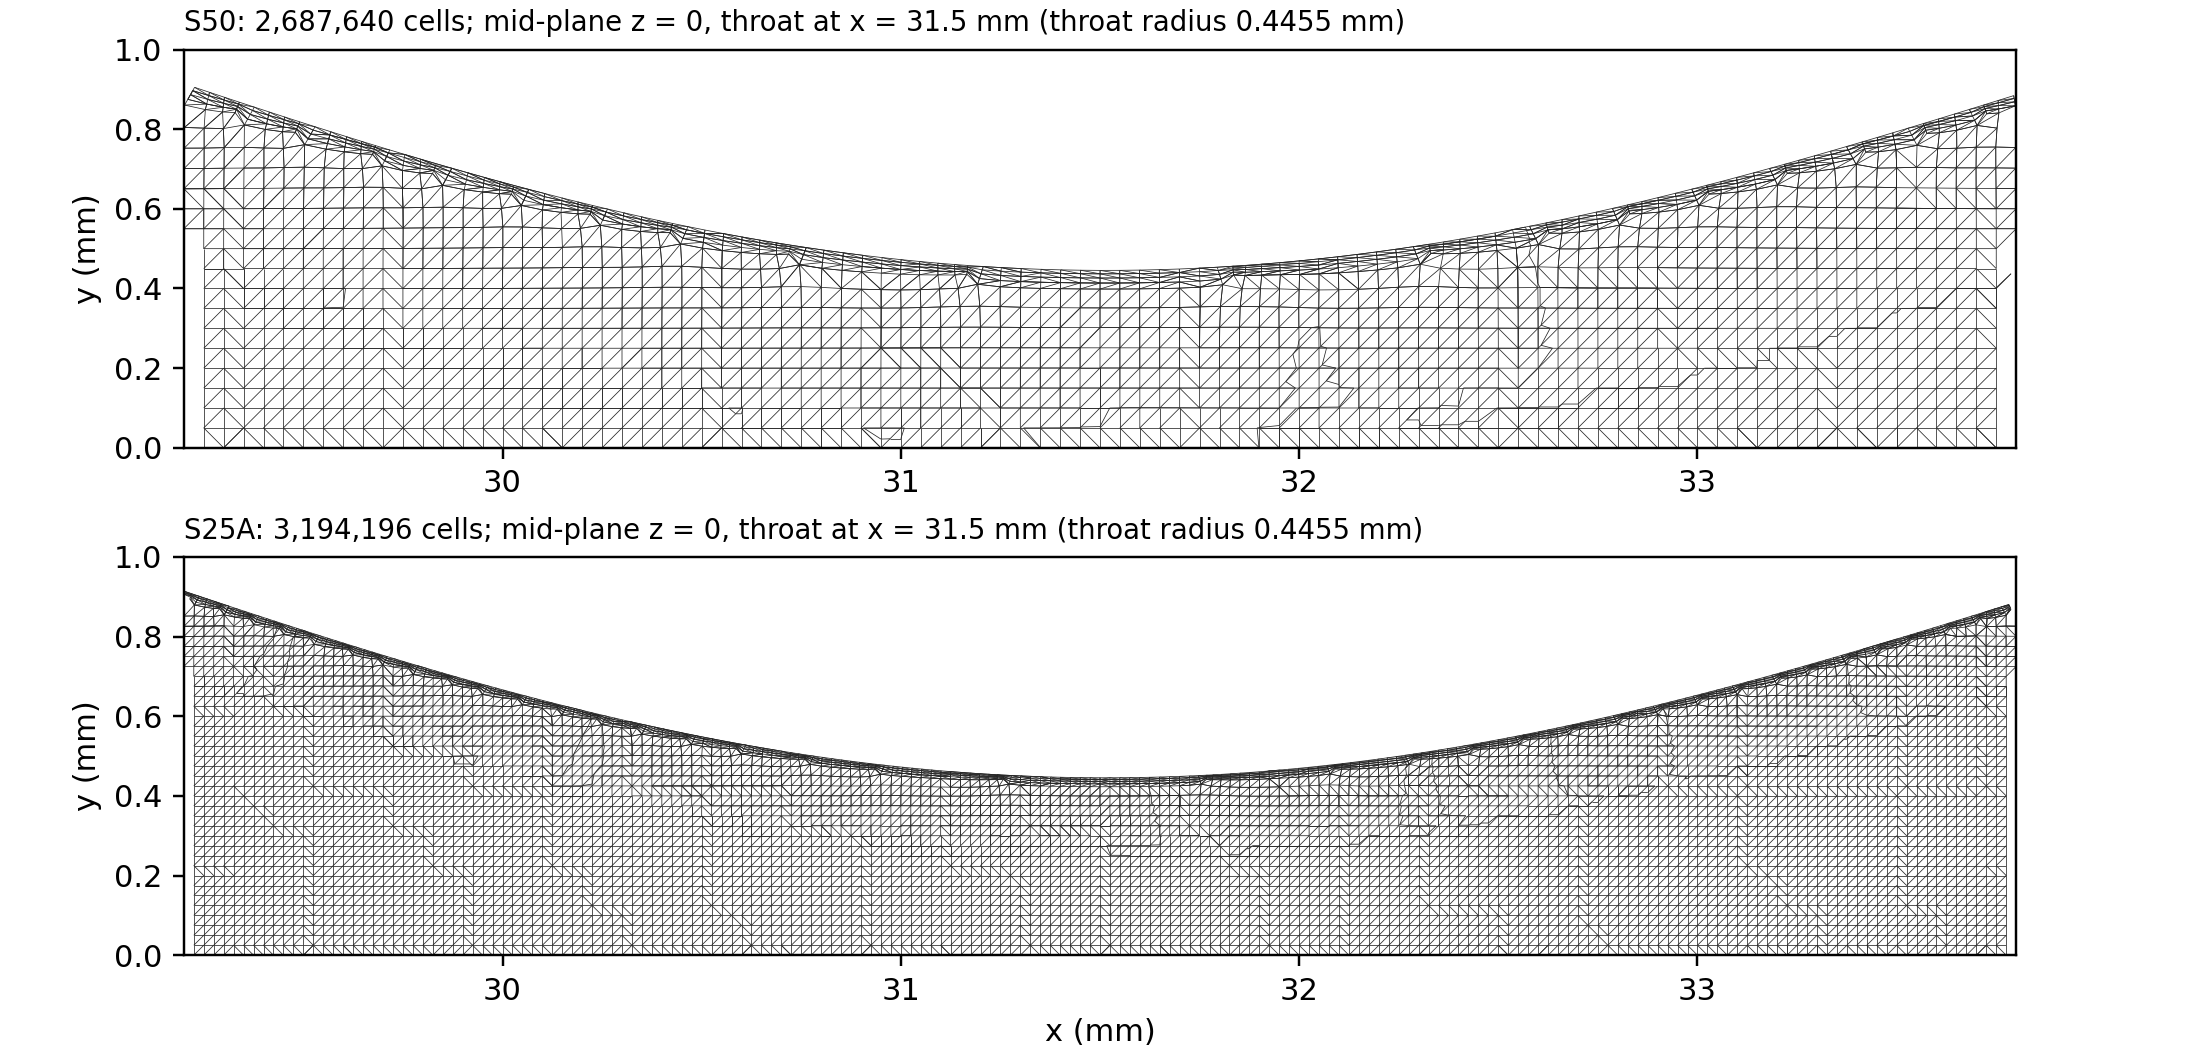
\includegraphics[width=\textwidth]{figures/cfd_u3d_mesh_closeup.png}
\caption[Throat-zone mesh of the U3D levels S50 and S25A (rebuilt 2026-10-02)]{\label{fig:u3d-mesh}Throat-zone mesh of the U3D levels S50 (50\,$\mu$m) and S25A (25\,$\mu$m): cell edges in the mid-plane $z=0$, $x=29.2$--33.8\,mm, with the four-layer boundary stack along the wall. The meshes were rebuilt on 2026-10-02 from the deposited code (same cell counts as the returned levels; \texttt{cartesianMesh} is not bitwise reproducible, so individual cells may differ from the returned meshes). The diagonal lines are where the plane cuts the cells' faces, not extra cells. Script \texttt{code\_\allowbreak{}from\_\allowbreak{}cfd/\allowbreak{}task1\_\allowbreak{}u3d/\allowbreak{}jet\_\allowbreak{}state\_\allowbreak{}check/\allowbreak{}viz\_\allowbreak{}u3d\_\allowbreak{}meshes.py}.}
\end{figure}

\textbf{Deviations and limits, disclosed.} (i) Budgets and thresholds: the SETTLED drift threshold of $2\times10^{-4}$ was fixed after W2 (drift $1.2\times10^{-4}$, passes with 40\% margin) and the drifting first W3 run had been seen, and the version-2.4 note said the W3 re-run would use 9000 iterations while it used 6000; the first wedge budget (3000) was too short for the finest level, so the SETTLED criterion and per-level budgets were pre-registered before the 3D runs; S25A and S25B were given 4000 iterations, S12A 6000 and, after S12A had settled at about 1500 iterations, S12B was reduced from 6000 to 3000 before it started (the settled criterion was applied at its end). (ii) $U_{3D}$ refers to the refined throat zone only: the lesion zone at 50\,$\mu$m and the regions beyond do not change between levels, and the geometry, the flow, and the steady laminar assumption are those of Stage A; a converged steady solution to $10^{-8}$ does not exclude an unsteadiness the steady solver cannot see. (iii) The boundary-layer stack ratio between levels is not exactly 2 (1.8 and 2.5; first cells 1.8 and 2.6): the family is not a strictly similar single-parameter refinement, so the fitted order and the GCI are conditional estimates, and three monotone values alone do not demonstrate an asymptotic regime. (iv) The setups were audited before the runs by one auditor (Gemini~3.8 Flash, two rounds), Astra being unavailable; GPT-6 Astra audited the finished study post hoc on 2026-09-26 (verdict: sound with caveats; it reproduced every returned FFR, band, drift, flow and Reynolds number and both GCI families from the raw monitors, and its findings are incorporated in this subsection, \S\ref{sec:followup-audit}). It also notes that 0.00055 is the uncertainty of the finest throat-zone solution for one geometry under steady laminar flow, not of the 50\,$\mu$m production base and not a physical-model uncertainty. (v) \textbf{Provisional (2026-10-01, \S\ref{sec:b3}).} The sten70 case admits two stable steady states whose FFR differs by 0.0015 on the A5 coarse mesh (three times $U_{3D}$); the fields of the five 3D levels were deleted after post-processing, so which state each level reached cannot be checked. The data are consistent with all levels being on the axisymmetric state (the zone families agree within $10^{-4}$ at each level and the finest 3D level agrees with the axisymmetric wedge within $10^{-4}$), but this is not a verification: $U_{3D}=0.00055$ stands as a provisional estimate until a jet-symmetry diagnostic exists for every level (a re-run with the fields kept). \textbf{Update 2026-10-02:} level S50, the coarsest level and the one that most affects the fitted order, was rebuilt from the deposited code (2{,}687{,}640 cells as before) and re-run with its fields kept (decision rule fixed beforehand in \texttt{u3d\_check/U3D\_CHECK\_DESIGN.md}): the jet is axisymmetric (centroid offset 0.0 and 0.4\,$\mu$m at $x=50$ and 56.5\,mm) and the FFR is 0.793363 against 0.793362 originally, so the original S50 was on the axisymmetric state. The same check of S25A (3{,}194{,}196 cells, 4000 iterations) gives an axisymmetric jet as well (offsets 0.0 and 0.1\,$\mu$m) and FFR 0.791103, identical to the original value to six digits. The two coarser levels of family A are therefore verified on the axisymmetric state; S12A, S12B and S25B remain checked only indirectly (their values continue the same monotone sequence, the two families agree within $10^{-4}$, and S12A agrees with the axisymmetric wedge within $10^{-4}$). A finest level on the other state is therefore unlikely but not excluded by a direct check.

\subsection{Task 3 of the 2026-09-24 work order: Gate M1 on the shipped scan-14 packages}
\label{sec:m1}
\textbf{Status and verdict (2026-09-26).} The three shipped packages of scan 14 (left LAD, proximal, 20\,mm lesion of 80\%DS: the unmodified lumen, the lesion, and the lesion plus a deleted side branch) were built end to end by a script without manual geometry repair, meshed, and solved in resistance mode and in prescribed-flow mode with a round trip (the tables of this subsection are regenerated from the data files); all solves converge, both boundary-condition modes are stable and the three round trips close to $\leq0.0051\%$ (criterion 0.5\%). \emph{Cohort membership (decision D5, replaces the earlier logged waiver).} The frozen CFD subset file (\texttt{CFD-SUBSET-FROZEN-2026-09-18.csv}, 30 rows, sha256 \texttt{8e0079a0\dots1118}, verified) reached this machine with the work order of 2026-09-26; the E0 assertion of the work order of 2026-09-24 (section 7, rule 2) was executed against it on 2026-09-26 and \textbf{passed}: (scan 14, left) is a member of the subset (\texttt{ffr\_discrete} 0.761, \texttt{healthy\_main} 0.951, LAD proximal, 20\,mm, 80\%DS). The cases were built while the file was absent and carry the waiver text in their \texttt{build\_info.json}; the assertion outcome does not change any of them. No 0D twin was run on scan 14 or any cohort scan (blinding). \emph{Verdict against the analysis-side decisions of 2026-09-26.} (D2) The \emph{relative} throat gate is decisive and passes ($+0.002$, $+0.022$, $+0.024$\%); the absolute check against $r_\text{target}$ is reported and fails ($+14.0$, $+19.5$, $-10.1$\%), which matters for the 3D-versus-0D comparison because the as-meshed throat (area-equivalent radius 0.2756\,mm) is larger than the package radius (0.2306\,mm), i.e.\ the 3D lesion is geometrically milder than the 0D one. (D3, D4) A self-intersection of the mask and strict-\texttt{checkMesh} failures are accepted only if no flagged entity lies within 2\,mm of the throat or of the measurement probe. \textbf{The clean case satisfies that rule; the baseline and T1 cases do not:} faces with poorly decomposing tets lie 1.43\,mm from the throat centre (1.38\,mm from the throat section; 12 flagged vertices lie within 2\,mm of the throat centre and 56 in the $\pm4$\,mm 25\,$\mu$m throat zone along the vessel) in both lesion meshes, and 2.55\,mm (2.07\,mm from the section) from the measurement probe; the concave cells and faces and the small-volume-ratio faces are at least 2.65\,mm away. By the rule as stated these two cases fail M1 and are reported, not repaired (Table~\ref{tab:m1-gates}); against the original mesh criterion of the CFD-arm specification (\texttt{checkMesh}: non-orthogonality $<70^\circ$, skewness $<4$, no negative volumes) all three meshes are clean (55.6$^\circ$, 1.85, none), and the 2\,mm rule concerns only the stricter \texttt{-allGeometry -allTopology} flags added by the work orders; the conditional verdict D6 (pass with deviations) therefore holds as measured for the clean case only, and the verdict for the lesion cases rests with the analysis side. The two conditions of D6 are met: the clean prescribed-flow round trip is done and the as-meshed radius files of all three cases are returned in the contract format, for both radius definitions (area-equivalent and inscribed); the junction nodes without a valid single-lumen section (17, 12 and 17 of 748, 706 and 748) carry blank radii, which the analysis-side ingestion treats as uncovered (the requested radius is kept). The kill clock of the work order (five working days without a scriptable path) was stopped by the analysis side; the day ledger is kept in the returned \texttt{NOTE\_long.md}.

\textbf{Build.} The frame (the NIfTI affine is RAS: $x$ and $y$ negated) puts 121/121 deletion points of the truncation and 163/163 of the missed-branch package in the lumen (0 without the flip). The shipped 6-connected deletion with protect radius $1.10\,r$, run once on the union of the sets, was executed verbatim and removes 1310 voxels (clean and baseline) and 2089 voxels (T1), the shipped numbers, leaving two connected components (Figure~\ref{fig:m1-mask}); the shipped ``erosion 25/40'' has no definition and could not be reproduced, and the retained LAD radius is unchanged except at the truncation end and, for T1, by 0.075, 0.045 and 0.023\,mm at three nodes next to the deleted branch. The surface was made by marching cubes, Taubin smoothing (\texttt{vmtksurfacesmoothing}, 30 iterations; no \texttt{vmtksurfaceremeshing}), planar outlet clips and straight extensions (inlet 13.01\,mm, outlets 3.29--4.73\,mm, taken as $5D$ and $3D$ with $D=2r_\text{mm}$ of the package; with the area-equivalent diameter of the clipped loops they would be 0.9--1.6 times as long). The lesion window was subdivided to edges $\leq0.0288$\,mm ($=r_\text{throat}/8$; about 1.1 M triangles) before the raised-cosine deformation, which follows the smoothing-spline path frames of the scan-837 pipeline (the package's literal nearest-node rule steps by up to 0.4\,mm across Voronoi cells).

\begin{figure}[H]
\centering
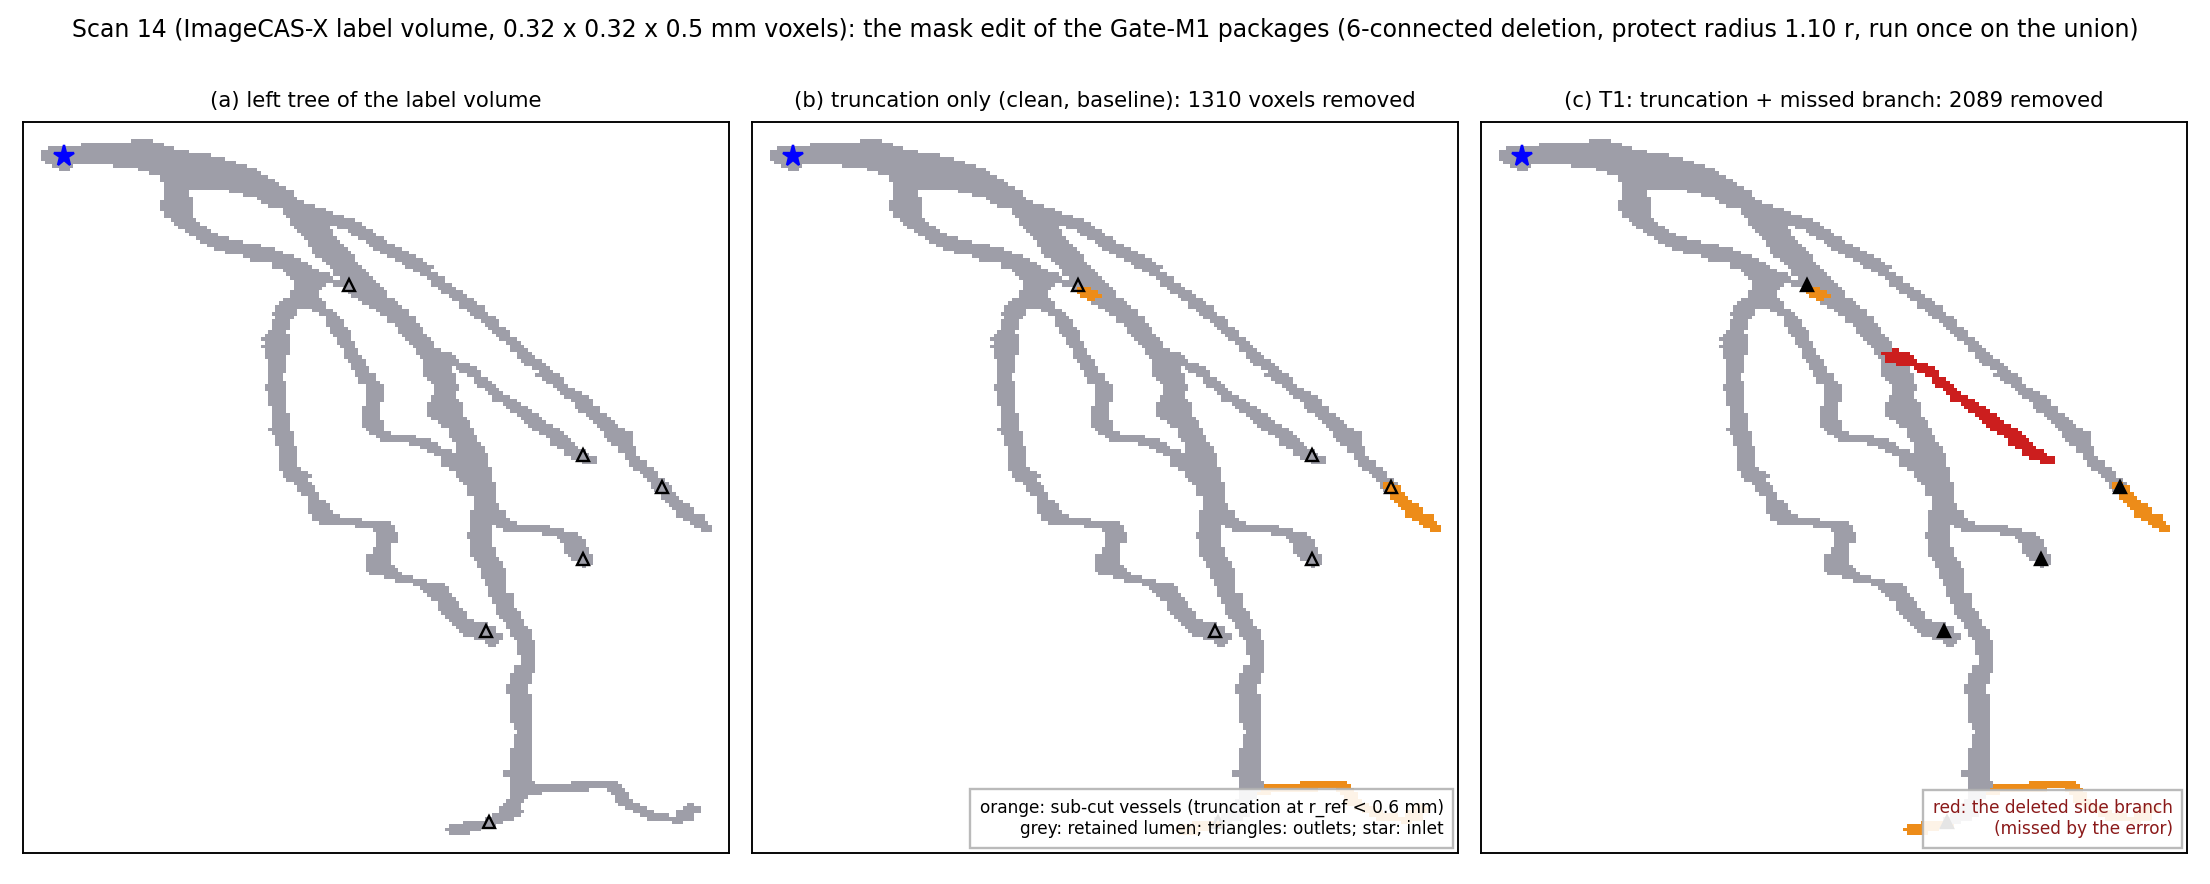
\includegraphics[width=\textwidth]{figures/img_m1_mask_edit.png}
\caption{\label{fig:m1-mask}Scan 14, label volume of the left tree (coronal maximum-intensity projection) and the mask edit of the packages. (a) The left tree with the inlet and the outlets of the baseline package. (b) The truncation at $r_\text{ref}<0.6$\,mm removes the sub-cut vessels (orange). (c) The T1 package removes, in the same run, a side branch (red) that the error ``missed''. The dataset provides the segmentation, not the CT intensities.}
\end{figure}

\begin{table}[H]
\centering
\caption{Gate M1, scan 14: geometry and mesh gates (P = pass, F = fail; clean / baseline / T1; the last three rows apply decisions D3 and D4 of the work order of 2026-09-26; distances are from the vertices of the flagged faces or cells to the probe point).}
\label{tab:m1-gates}
\small
\begin{tabular}{p{5.6cm}p{7.6cm}p{2.2cm}}
\toprule
gate & result & verdict \\
\midrule
frame flip, deletion points in the lumen & 121/121, 121/121, 163/163 (0 without flip) & P \\
voxels removed, components after the edit & 1310, 1310, 2089 (= shipped), 2 & P \\
clip loops with outward normals & 7, 7, 6 (expected 7, 7, 6) & P \\
final surface closed, one part, positive volume & 77 k / 1.17 M / 1.17 M triangles & P \\
lesion purity, fold-over, edge $\leq r_\text{throat}/8$ & min normal dot 0.37, 100\% of window edges & P \\
throat, \emph{relative} (as built / undeformed against \texttt{radial\_scale} 0.2081) & $+0.002$ / $+0.022$ / $+0.024$\% (three radius definitions) & P (decisive, deviation) \\
throat, \emph{literal absolute} against $r_\text{target}=0.2306$\,mm & $+14.0$ / $+19.5$ / $-10.1$\% (inscribed circle / area-equivalent / sphere at the axis) & \textbf{F} \\
\texttt{surfaceCheck -checkSelfIntersection} (positive control flagged) & 14 / 16 / 8 locations (present in the raw marching-cubes surface in all three) & \textbf{F} \\
strict \texttt{checkMesh}: nearest flagged entity to the throat probe (D4) & 2.95 / 1.43 / 1.43\,mm (concave faces / face tets / face tets); 1.38\,mm from the throat section & P / \textbf{F} / \textbf{F} \\
strict \texttt{checkMesh}: nearest flagged entity to the measurement probe (D4) & 2.55 / 2.55 / 2.55\,mm (face tets; 2.07\,mm from the section) & P / P / P \\
self-intersection accepted (D3: raw surface intersects and no flagged entity within 2\,mm) & 2\,mm rule met only by the clean case & P / \textbf{F} / \textbf{F} \\
\bottomrule
\end{tabular}
\end{table}

\textbf{Failed gates, reported as results.} (i) \emph{Self-intersection}: present in the raw marching-cubes surface, hence caused by the mask, not by smoothing or clipping: a 1-voxel-wide whisker of mask at LAD node 285 (all cases) and a thin D1 of 1.7 voxels at node 133 (clean and baseline; gone in T1 where the branch is deleted). Nothing was repaired; cfMesh meshed the surfaces and no concave cell or face and no small-volume-ratio face lies within 2\,mm of either site; 81 points of faces with poorly decomposing tets do lie within 2\,mm of the two whisker sites in the clean and baseline meshes (none in T1; point counts, not face counts); under decision D3 the intersection is accepted only where the strict-check flags are farther than 2\,mm from the throat and the measurement probe, which the lesion meshes do not satisfy (verdict above). (ii) \emph{Literal throat check}: the package radius (vmtk maximum inscribed sphere on the dataset surface) and this marching-cubes surface differ by $-0.3\%$ in the median and by $-10$ to $+8\%$ (10th to 90th percentile) per node, so the as-built throat cannot reproduce $r_\text{target}$ within 1\% whatever the definition; the gate that was made decisive is therefore the \emph{relative} one (as built over undeformed, against the package's own \texttt{radial\_scale}), which passes to 0.03\%. The analysis side confirmed this reading (decision D2: the relative check is decisive, the absolute check is reported in every return and does not reject a case).

\textbf{Meshes.} cfMesh with four boundary layers of ratio 1.2 (the scan-837 meshes used three), a 25\,$\mu$m zone of $\pm4$\,mm along the LAD around the throat, 50\,$\mu$m zones at the inlet and outlets, and 100\,$\mu$m and coarser elsewhere: 3.89 M (clean), 3.66 M (baseline) and 3.49 M cells (T1) in 1:41--1:57\,min on the host (peak 2.8\,GB); all inlet and outlet patches present; standard \texttt{checkMesh} OK; the strict check fails three checks per mesh (about 1000 faces of poor face-decomposition tets, 41--52 concave cells and 19--30 small-volume-ratio faces), spread over the tree and at the zone ends: the concave cells and faces and the small-volume-ratio faces lie at least 2.65\,mm from the throat, but the faces with poor decomposition tets come as close as 1.43\,mm to it in the baseline and T1 meshes, with 12 flagged vertices within 2\,mm of the throat centre and 56 in the $\pm4$\,mm 25\,$\mu$m throat zone (none in the clean mesh; vertex counts, not face counts), so the localisation does not show that the failures are harmless to the flow; maximum non-orthogonality 55.6$^\circ$, skewness 1.85, aspect ratio 11. The lesion meshes hold 36 (minimum) and 39.5 (median) cells across the 0.55\,mm throat chord (requirement $\geq12$), a p95 cell size of 25.7\,$\mu$m and a four-layer stack of 16.5\,$\mu$m at the throat; the as-meshed throat has an area-equivalent radius of 0.2756\,mm (Figure~\ref{fig:m1-results}b). cfMesh writes the inlet and outlet patches with type \texttt{wall}; only that keyword was changed to \texttt{patch} in each \texttt{boundary} file.

\textbf{Solves.} Both boundary-condition modes use the audited setups of this report (coded resistance boundary condition with $G=R/R_\text{own}$ relaxation, $R_\text{own}$ from the package centreline radii; prescribed mode with \texttt{flowRateOutletVelocity} on every outlet at once and zero-gradient pressure; inlet total pressure of the package; 16 ranks, one solve at a time, fixed budget of 3000 iterations, laminar). The audited relaxation rule gives 0.0036--0.040 for the outlets (time constants up to about 280 iterations); it did not prevent convergence in 3000 iterations. Table~\ref{tab:m1-solves} lists the solves, Table~\ref{tab:m1-flows} the resistance-mode flows against the package flows, Table~\ref{tab:m1-roundtrip} the round trips; Figure~\ref{fig:m1-walls} shows the wall pressure and Figure~\ref{fig:m1-cpr} the pressure along the LAD. The throat Reynolds number is computed from the section flux at the throat probe (an earlier value from an infinite sampling plane that also cut other branches was wrong and was corrected after the post-hoc audit): 123 (baseline, resistance), 106 (baseline and T1, prescribed), 60 (T1, resistance) and 29 (resistance) and 22 (prescribed) at the would-be throat station of the clean tree, so the steady laminar assumption is comfortably within range for scan 14.

%%M1_TABLES_BEGIN
\begin{table}[H]
\centering
\caption{Scan-14 Gate-M1 solves (16 ranks each, one at a time, fixed budget 3000 iterations, strict verdict as stated; the throat Reynolds number is the section flux at the throat probe, at the would-be throat station for the clean tree).}
\label{tab:m1-solves}
\small
\resizebox{\textwidth}{!}{\begin{tabular}{llrrrrrrr}
\toprule
case & BC mode & cells & verdict & inflow (mL/s) & throat $Re$ & wall (h) & RAM (GB) & round trip max error (\%) \\
\midrule
clean & resistance & 3{,}889{,}165 & converged & 0.7119 & 29 & 2.34 & 6.1 & -- \\
clean & prescribed & 3{,}889{,}165 & converged & 0.6490 & 22 & 2.08 & 6.1 & 0.0013 \\
baseline (80\%DS) & resistance & 3{,}657{,}147 & converged & 0.6817 & 123 & 2.31 & 5.9 & -- \\
baseline (80\%DS) & prescribed & 3{,}657{,}147 & converged & 0.6490 & 106 & 2.17 & 5.8 & 0.0013 \\
T1 (lesion; branch deleted) & resistance & 3{,}485{,}528 & converged & 0.5796 & 60 & 2.09 & 5.7 & -- \\
T1 (lesion; branch deleted) & prescribed & 3{,}485{,}528 & converged & 0.6490 & 106 & 2.09 & 5.6 & 0.0051 \\
\bottomrule
\end{tabular}}
\end{table}

\begin{table}[H]
\centering
\caption{Resistance mode with the package resistances (\texttt{bc\_A}): 3D outlet flow against the package target flow (\texttt{bc\_C}); a positive deviation means that the 3D tree delivers more than the target.}
\label{tab:m1-flows}
\small
\begin{tabular}{llrrr}
\toprule
case & outlet & $Q_\text{target}$ (mL/s) & $Q_\text{3D}$ (mL/s) & deviation (\%) \\
\midrule
clean & out\_160 & 0.0953 & 0.1272 & +33.5 \\
clean & out\_425 & 0.1044 & 0.1054 & +1.0 \\
clean & out\_600 & 0.0782 & 0.1039 & +32.8 \\
clean & out\_639 & 0.1126 & 0.1122 & -0.3 \\
clean & out\_742 & 0.1234 & 0.1258 & +1.9 \\
clean & out\_868 & 0.1351 & 0.1374 & +1.7 \\
baseline & out\_160 & 0.0953 & 0.1105 & +16.0 \\
baseline & out\_425 & 0.1044 & 0.1054 & +1.0 \\
baseline & out\_600 & 0.0782 & 0.0903 & +15.4 \\
baseline & out\_639 & 0.1126 & 0.1122 & -0.3 \\
baseline & out\_742 & 0.1234 & 0.1259 & +2.0 \\
baseline & out\_868 & 0.1351 & 0.1374 & +1.7 \\
T1 & out\_383 & 0.1044 & 0.1054 & +1.0 \\
T1 & out\_558 & 0.1735 & 0.0985 & -43.2 \\
T1 & out\_597 & 0.1126 & 0.1123 & -0.3 \\
T1 & out\_700 & 0.1234 & 0.1259 & +2.0 \\
T1 & out\_826 & 0.1351 & 0.1375 & +1.8 \\
\bottomrule
\end{tabular}
\end{table}

\begin{table}[H]
\centering
\caption{Prescribed-flow round trip on scan 14: every outlet flow prescribed at once (\texttt{bc\_C}), $R_i=(\bar p_i-P_v)/Q_i$ derived, re-imposed in resistance mode; error of the re-solved flow against the prescribed one (criterion 0.5\%), and derived resistance against the package resistance (\texttt{bc\_A}).}
\label{tab:m1-roundtrip}
\small
\begin{tabular}{llrrr}
\toprule
case & outlet & $Q$ (mL/s) & round-trip error (\%) & $R_\text{derived}/R_\text{bc\_A}-1$ (\%) \\
\midrule
baseline & out\_160 & 0.0953 & +0.0000 & +19.5 \\
baseline & out\_425 & 0.1044 & -0.0004 & +1.0 \\
baseline & out\_600 & 0.0782 & -0.0003 & +19.0 \\
baseline & out\_639 & 0.1126 & -0.0013 & -0.3 \\
baseline & out\_742 & 0.1234 & -0.0002 & +2.1 \\
baseline & out\_868 & 0.1351 & +0.0000 & +1.8 \\
T1 & out\_383 & 0.1044 & -0.0004 & +1.0 \\
T1 & out\_558 & 0.1735 & -0.0051 & -47.5 \\
T1 & out\_597 & 0.1126 & -0.0013 & -0.3 \\
T1 & out\_700 & 0.1234 & -0.0002 & +2.1 \\
T1 & out\_826 & 0.1351 & +0.0000 & +1.8 \\
clean & out\_160 & 0.0953 & +0.0000 & +34.2 \\
clean & out\_425 & 0.1044 & -0.0004 & +1.0 \\
clean & out\_600 & 0.0782 & -0.0003 & +33.6 \\
clean & out\_639 & 0.1126 & -0.0013 & -0.3 \\
clean & out\_742 & 0.1234 & -0.0002 & +2.1 \\
clean & out\_868 & 0.1351 & +0.0000 & +1.8 \\
\bottomrule
\end{tabular}
\end{table}

%%M1_TABLES_END

\begin{figure}[H]
\centering
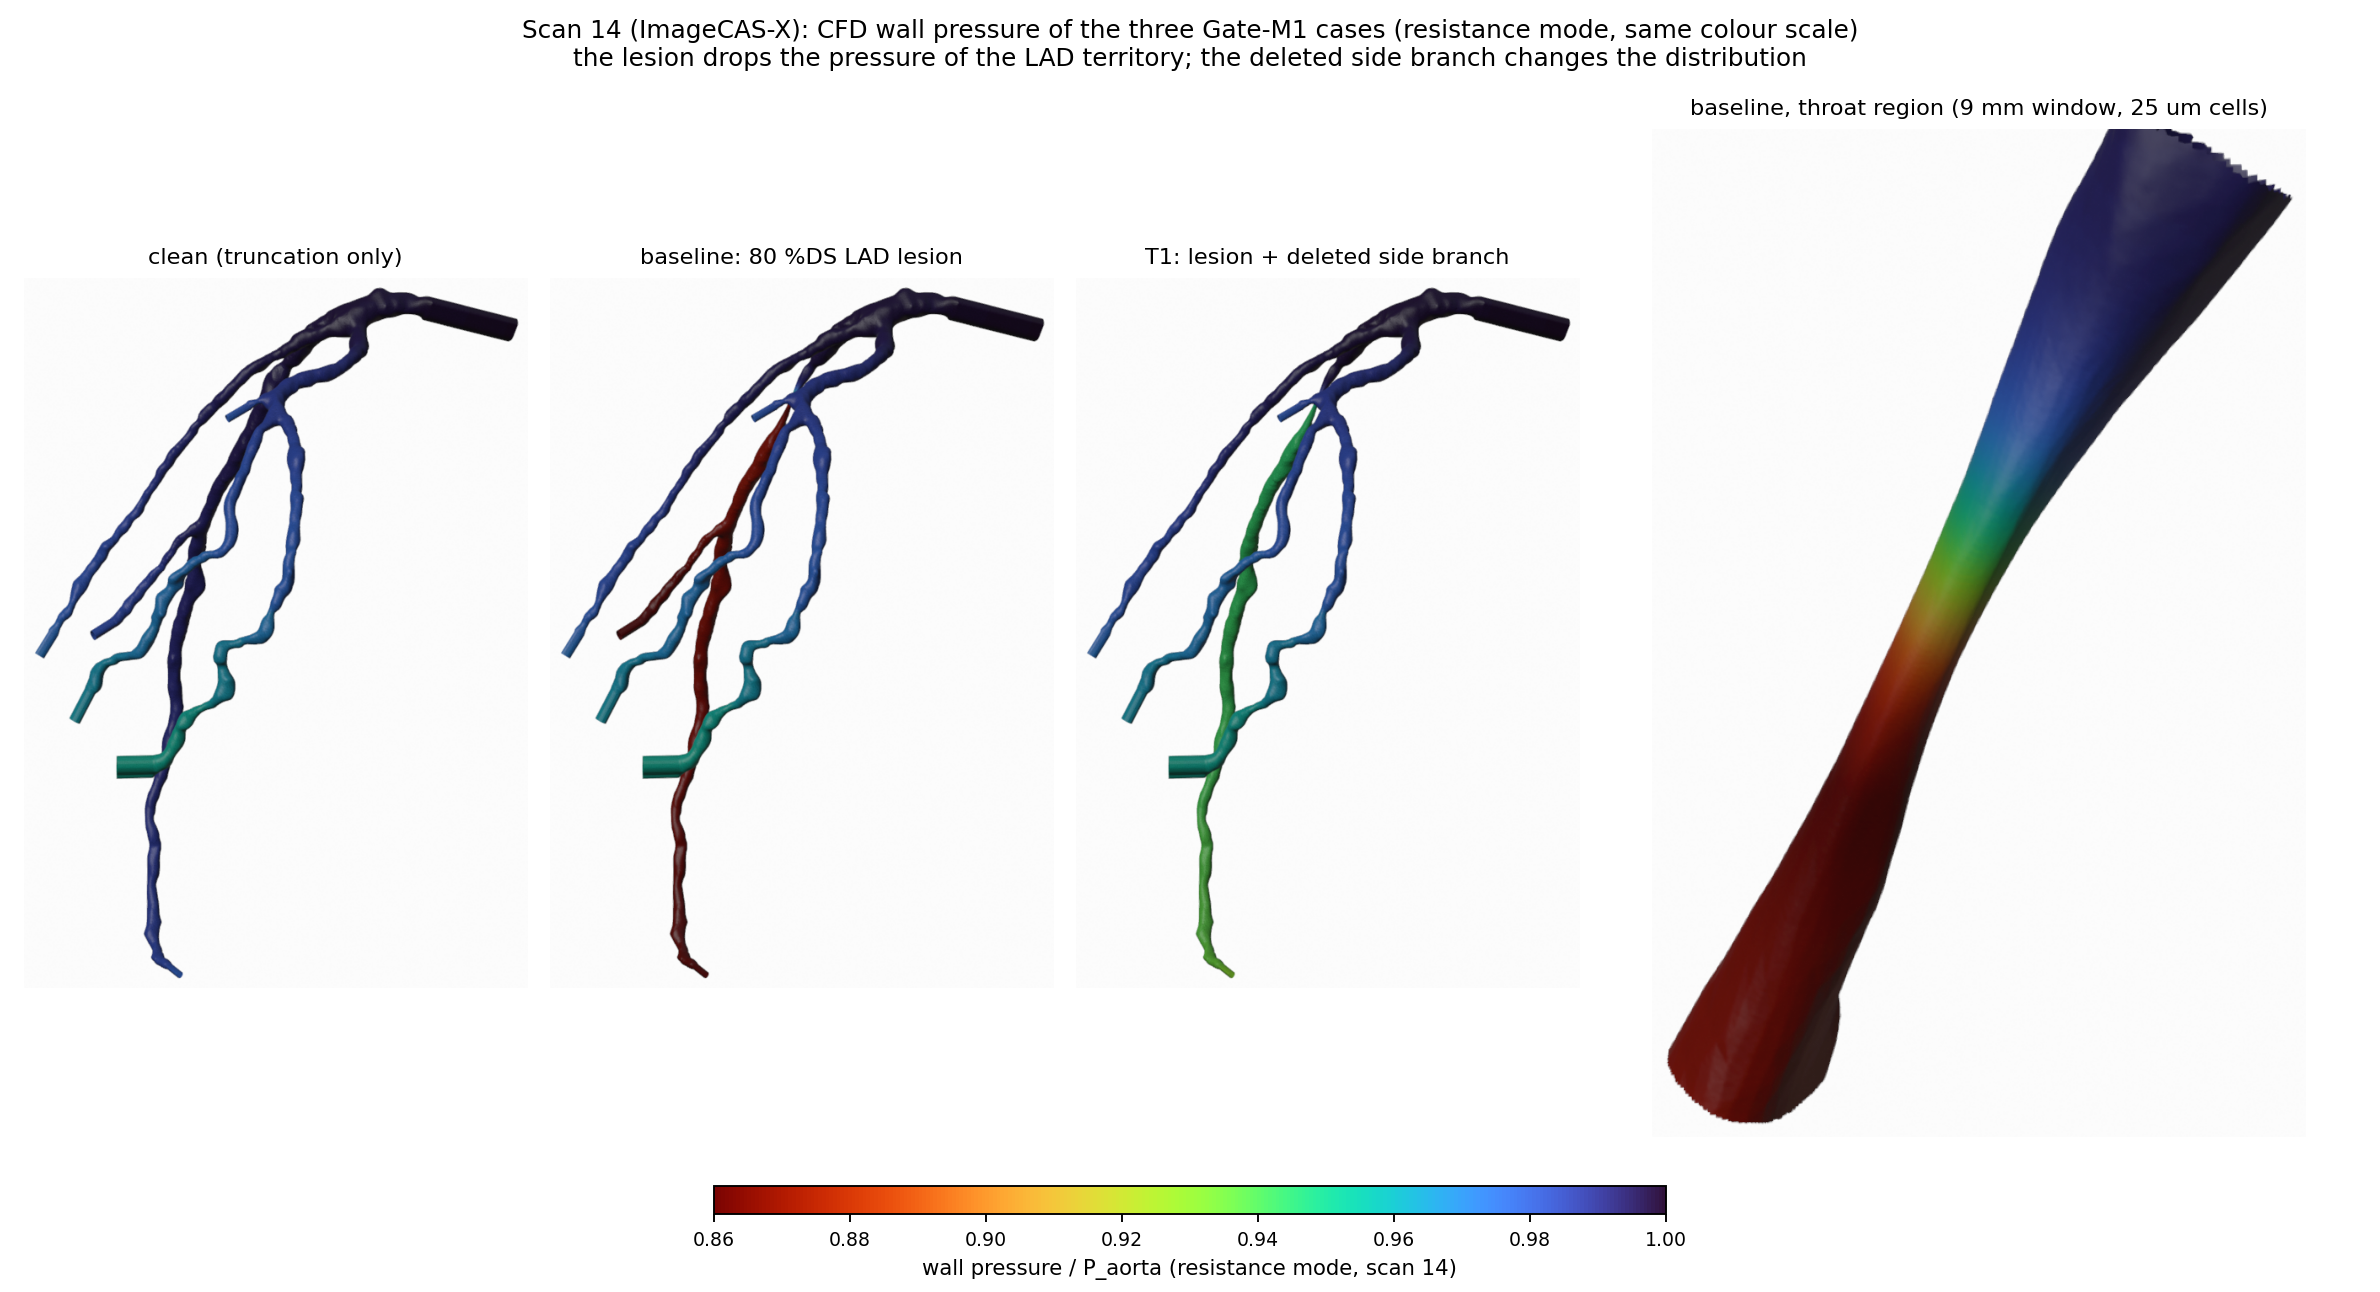
\includegraphics[width=\textwidth]{figures/img_m1_wall_pressure.png}
\caption{\label{fig:m1-walls}Scan 14, wall pressure over aortic pressure of the three cases in resistance mode (same colour scale; Blender, Workbench engine). The 80\%DS lesion drops the pressure of the LAD territory to 0.86--0.87 of the aortic pressure; in T1 the deleted side branch changes the distribution (out\_558, whose full-territory target cannot be delivered, is depressed). Right: the throat region of the baseline mesh.}
\end{figure}

\begin{figure}[H]
\centering
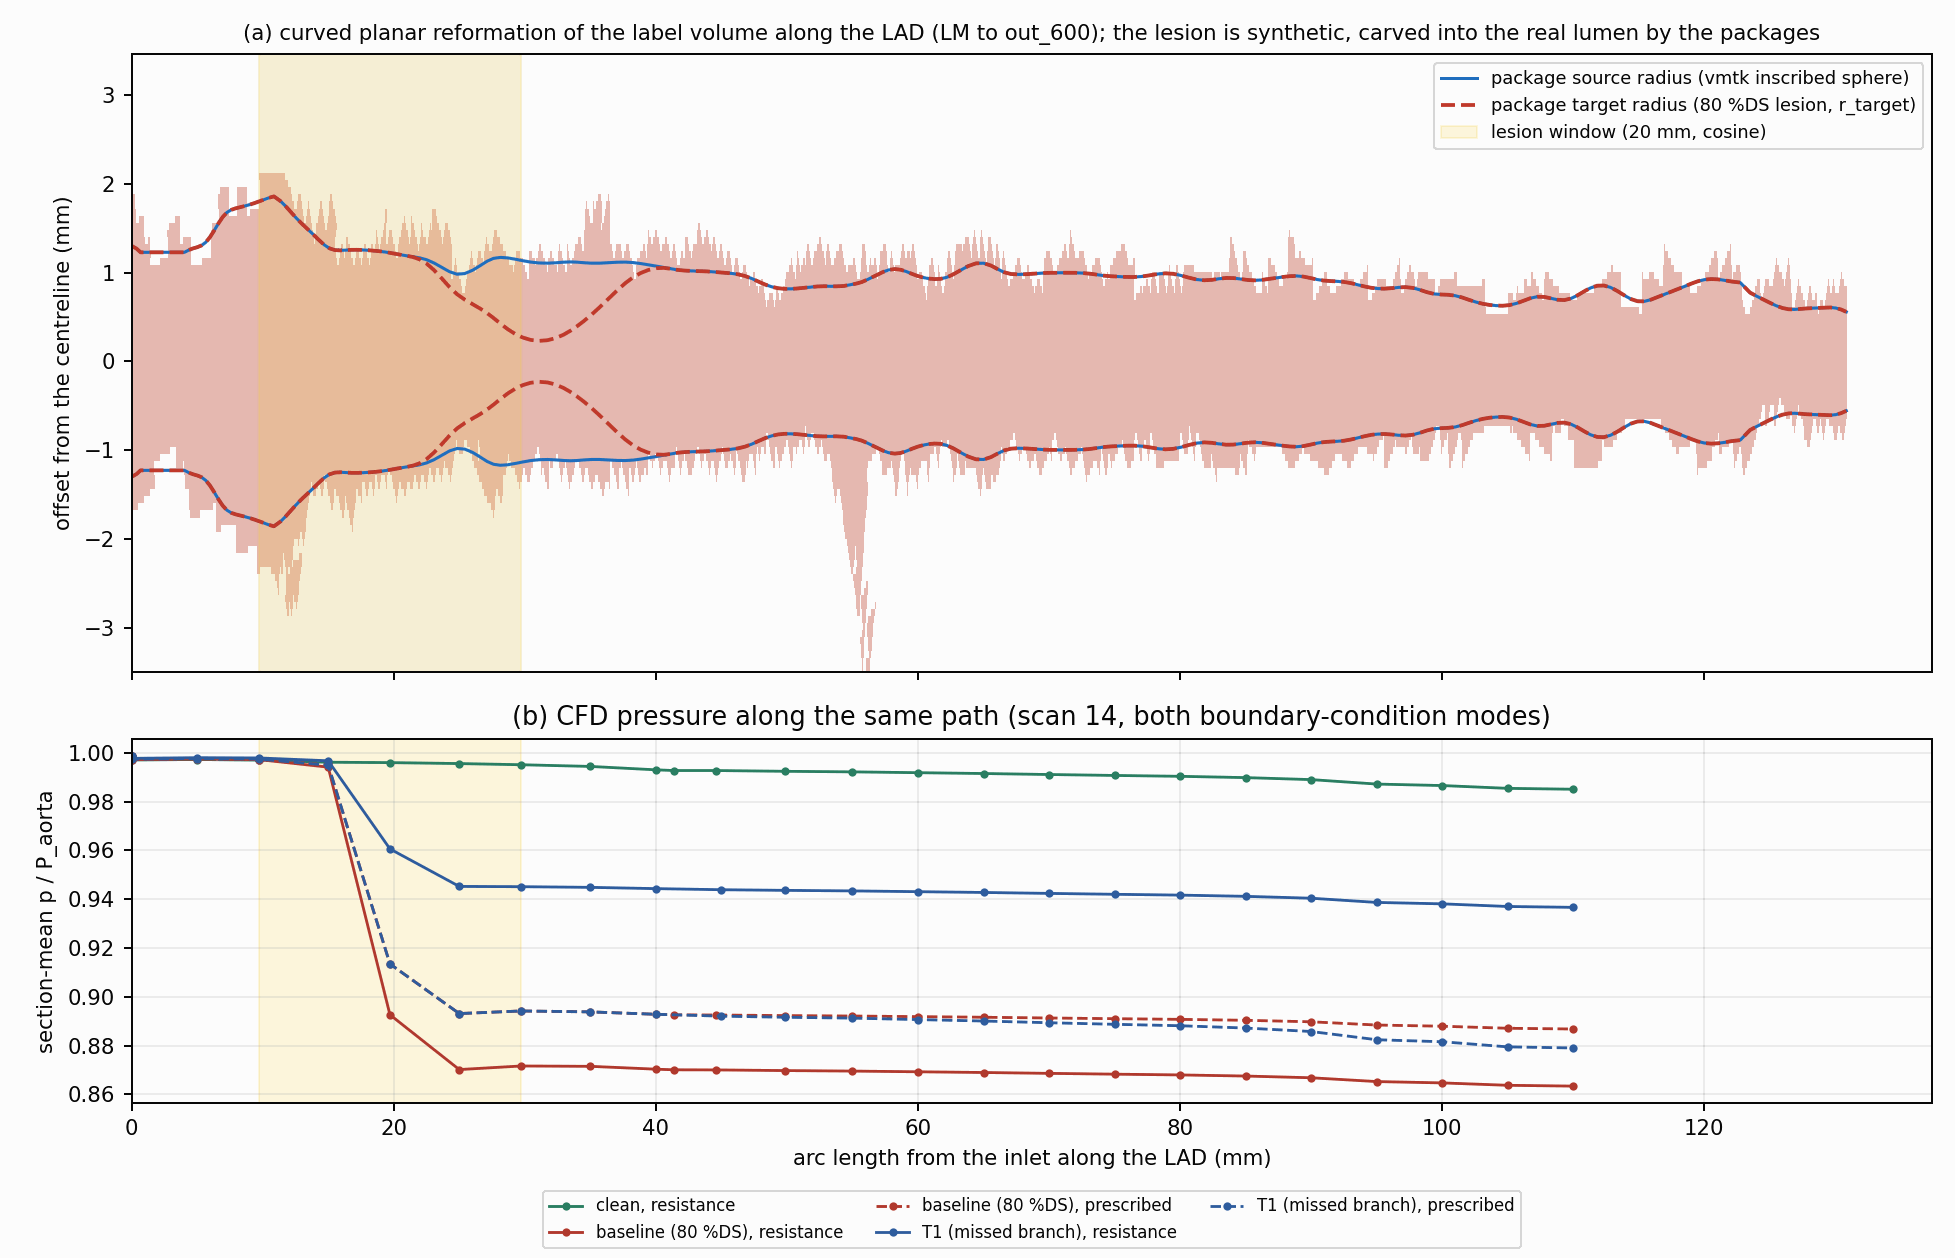
\includegraphics[width=\textwidth]{figures/img_m1_cpr.png}
\caption{\label{fig:m1-cpr}(a) Curved planar reformation of the scan-14 label volume along the LAD (LM to out\_600) with the radii of the package: the source radius (blue) and the target radius of the 80\%DS lesion (red dashed), which is synthetic and carved into the real lumen. (b) Section-mean pressure of the CFD solves along the same path in both boundary-condition modes.}
\end{figure}

\begin{figure}[H]
\centering
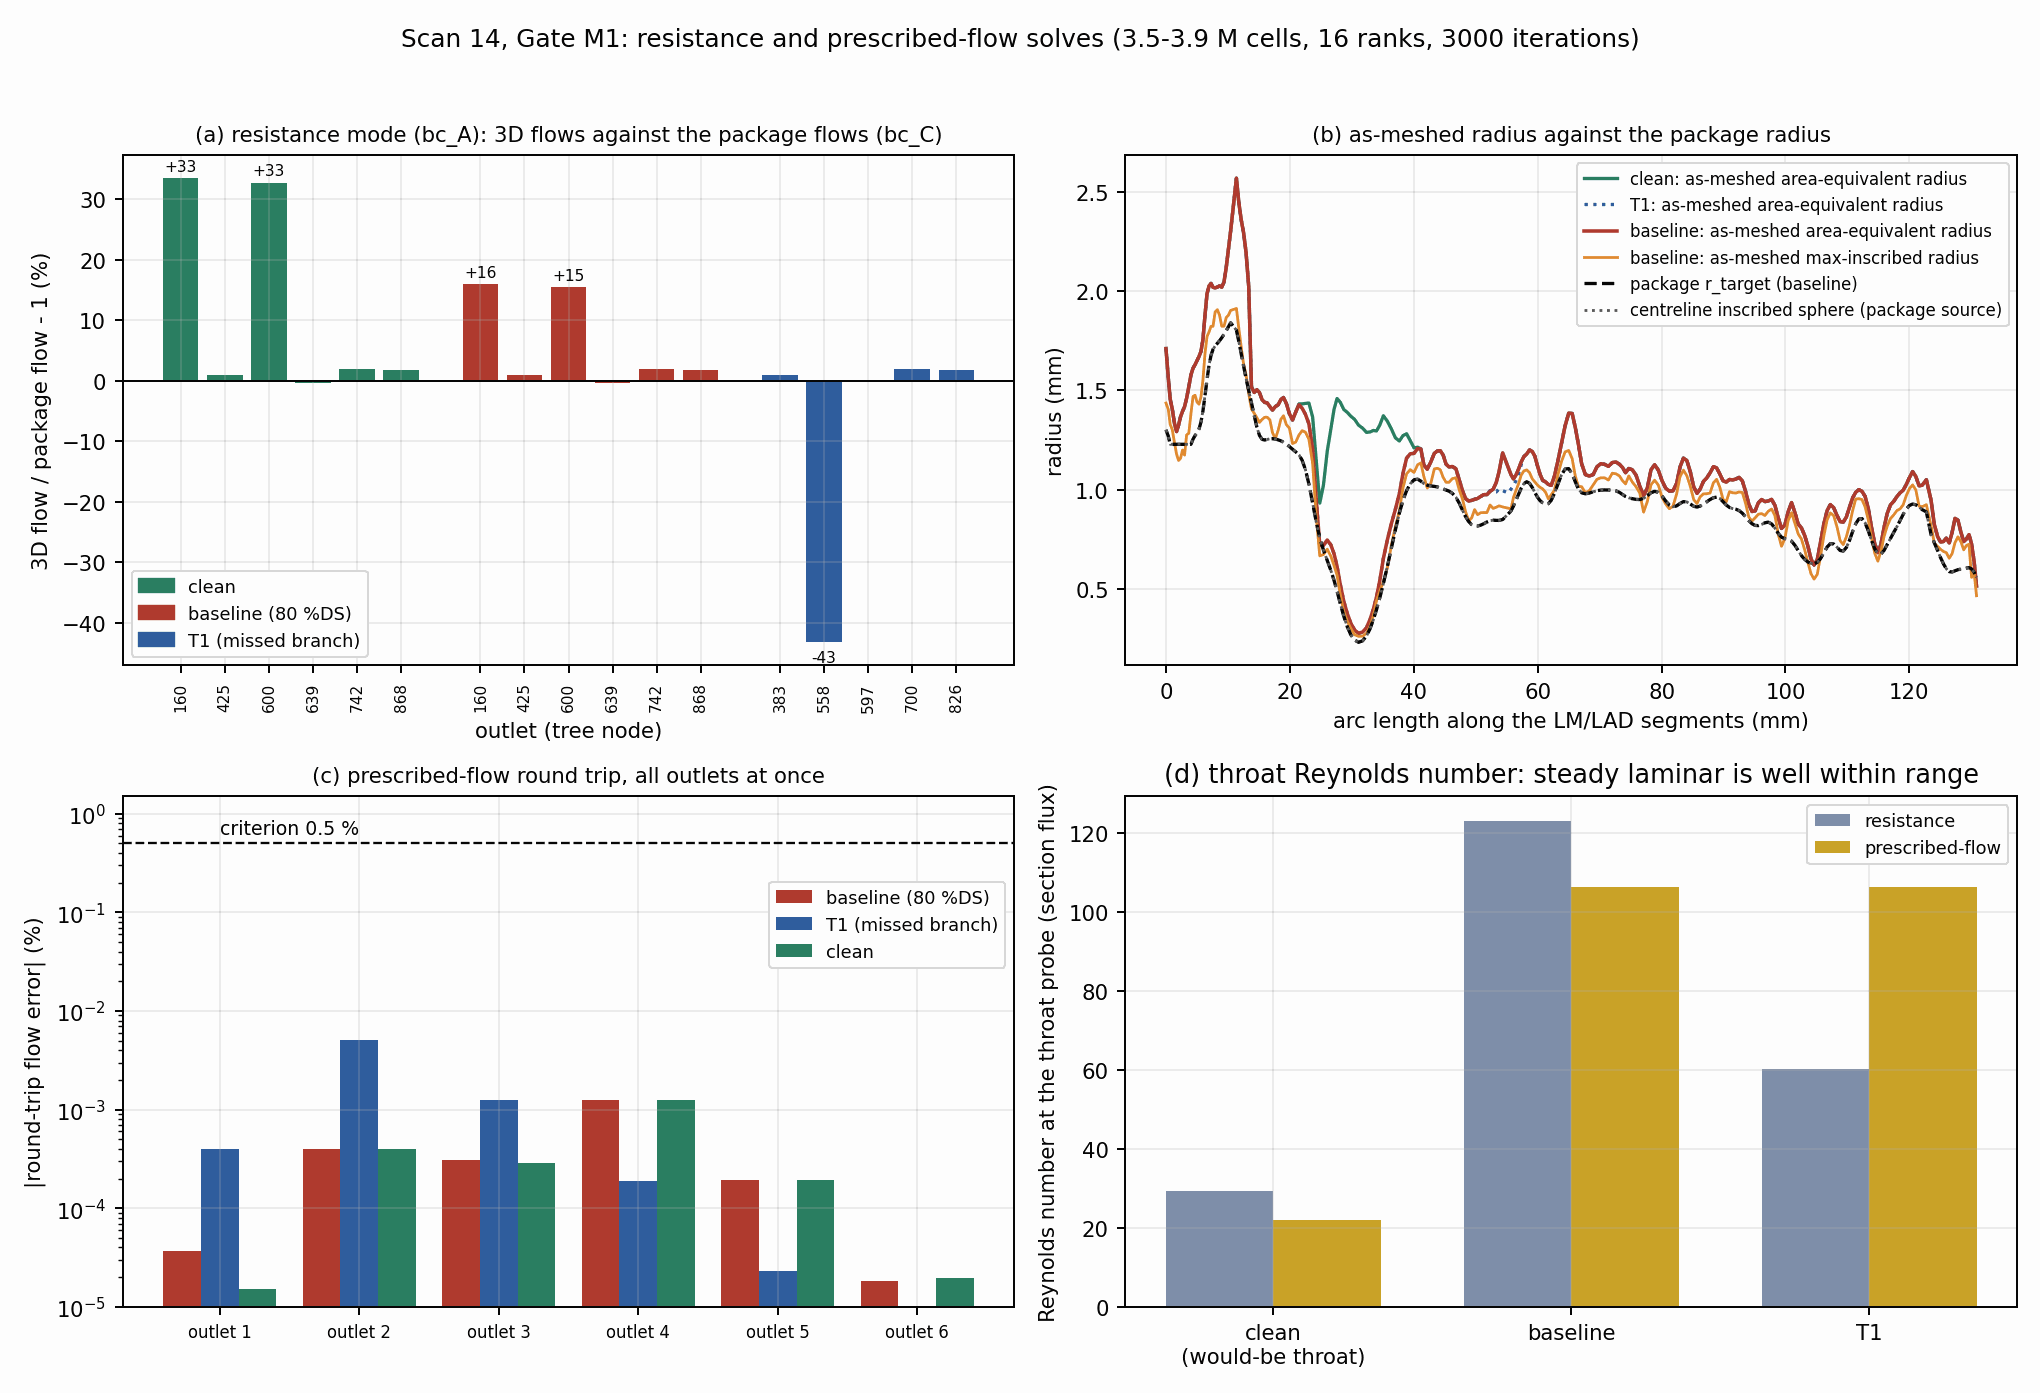
\includegraphics[width=\textwidth]{figures/cfd_m1_results.png}
\caption{\label{fig:m1-results}Scan 14, Gate M1: (a) resistance mode, 3D outlet flows against the package flows (\texttt{bc\_C}); (b) as-meshed area-equivalent and maximum-inscribed radius along the LM/LAD segments against the package radius; (c) round-trip flow errors of the prescribed-flow mode (all outlets at once); (d) throat Reynolds number from the section flux.}
\end{figure}

\textbf{Findings.} (i) \emph{Flow split.} Reading corrected by the analysis side (erratum E1 of 2026-09-26): the \texttt{bc\_A} and \texttt{bc\_C\_flows} files of the clean package are byte-identical to those of the baseline package, i.e.\ they are the boundary conditions of the tree \emph{with} the 80\%DS lesion, so a lesion-free lumen given lesion-state resistances over-delivers, by construction, to the territory that the lesion was throttling; the +33\% at territory~0 of the clean tree (out\_160 and out\_600: 0.0953 against 0.1272 and 0.0782 against 0.1039\,mL/s) is therefore not a 0D-versus-3D finding, and the package gives no flow target for a lesion-free lumen: the clean case is reported as a geometry and pipeline check only. The comparable number is the baseline: with the package resistances the 3D lesioned tree delivers $+16.0\%$ (out\_160) and $+15.4\%$ (out\_600) more than the package targets to the lesioned territory, and $\leq2\%$ elsewhere; attribution between the lesion geometry (the as-meshed throat radius is larger than the package radius, decision D2) and model fidelity is left to the analysis side, and no 0D twin was built to attribute it (blinding). No discrepancy was found in the checked boundary-condition values and outlet mapping ($R_\text{derived}/R_{\text{bc\_A}}=1.00000$ on all outlets in resistance mode; the deviating outlets are exactly territory~0 of \texttt{bc\_C}); satisfying the applied resistance law cannot by itself exclude a wrong physical mapping or a geometry problem. (ii) \emph{T1.} Erratum E2 of the work order of 2026-09-26 (it replaces the sentence of the package README that \texttt{bc\_A}$\times$\texttt{bc\_C} reconstructs the clean outlet pressures, true only for the clean and baseline packages): the T1 target of out\_558 is the \emph{full} territory-0 flow of the clean tree, 0.1735\,mL/s including the share of the deleted branch, whereas the surviving-outlet share is 0.0782\,mL/s (ratio 2.218); that target is not reachable at that resistance by design ($P_v+R\,Q$ would be 19.1\,kPa, above the aortic pressure of 12.0\,kPa), and the $-43\%$ (0.098 of 0.173\,mL/s) is the expected result of Protocol~A. In prescribed mode the flow is delivered with that outlet at 0.863 of the aortic pressure (labelled pilot: its targets are provisional). (iii) \emph{Round trips.} Prescribing all outlets at once was stable from rest without a ramp; the re-imposed resistances reproduce the prescribed flows to $\leq0.0013\%$ (baseline and clean) and $\leq0.0051\%$ (T1), against the 0.5\% criterion. This is a fixed-point and stability test of the relaxed coded condition (the resistances are derived from the same converged solution), not a validation of the package flows; for the clean case the prescribed flows are the lesion-state targets (E1), so its round trip is a stability test only. (iv) \emph{Cost.} About 2.1--2.3\,h and 5.7--6.1\,GB per 3.5--3.9\,M-cell solve at 16 ranks for the fixed budget of 3000 iterations, about 13 times the estimate of the CFD-ARM specification; the geometry build takes 3--9\,min per case and the meshing 2--5\,min including the gates, so the whole path from mask to converged solution is scripted and takes about 2.5\,h per case and mode. The returned table \texttt{settle\_iterations.csv} applies the $U_{3D}$ settled criterion (drift over 500 iterations $\leq2\times10^{-4}$, last-100 band $\leq10^{-4}$) plus flow bands and BC errors $<0.1\%$ to every real-lumen steady solve, on the pressure of the outlet on the LAD path (no solve monitored the measurement probe; the table is labelled 	exttt{PROXY\_NOT\_B1} because this substitution, and the replacement of the outlet-flow bands by outlet-pressure bands in prescribed-flow mode, are not authorised by the work order, so it is no production stopping rule until the analysis side agrees): the nine scan-14 solves first meet it after 931--1235 iterations in resistance mode (about half of the wall clock of the fixed budget) and after 509--551 in prescribed-flow mode, and the FFR proxy at that iteration differs from its final value by at most $9\times10^{-5}$ in resistance mode but by $2.2\times10^{-4}$ (baseline, T1) in prescribed-flow mode, where stopping at the first satisfaction is therefore too early (from iteration 771: $1.1\times10^{-4}$). \textbf{Limits:} one scan; the D3/D4 conditions are not met by the two lesion meshes as reported; the strict mesh check is localised, not eliminated; the setups were audited before the runs by Gemini~3.8 Flash alone (Astra being at its usage limit) and after the fact by Fable~5.1 as a stand-in and by GPT-6 Astra (findings incorporated, \S\ref{sec:followup-audit}).

\subsection{Task B3 of the 2026-09-26 work order: smoke test, and a second steady state of the sten70 case}
\label{sec:b3}
\textbf{What happened.} The smoke test (\texttt{code\_from\_cfd/smoke\_test}: the Stage A sten70 vessel on the A5 coarse recipe, 198{,}252 cells, steady laminar \texttt{simpleFoam}, coded resistance outlet, 3000 iterations on 8 ranks) was run on the CFD machine on 2026-10-01 to write its reference. It converged by iteration 1000 to an outlet flow of $1.17825\times10^{-6}$\,m$^3$/s and stayed there to 12{,}000 iterations, $+0.369\%$ above the returned A5 coarse value ($1.17392\times10^{-6}$), outside the 0.1\% criterion. Dictionaries, initial fields, STL (sha256) and cell count were identical to the returned run, and the returned value was reproduced to $-0.0016\%$ by re-running the \emph{archived} mesh of 2026-09-18 on the same machine, so the software environment is not the cause.

\textbf{Diagnosis: two stable steady states.} The case has two steady solutions of the discrete equations on the same mesh: an axisymmetric jet (outlet flow $1.178251\times10^{-6}$\,m$^3$/s, FFR at $x=56.5$\,mm 0.78248) and a jet deflected towards the wall downstream of the throat (flow $1.173903\times10^{-6}$, FFR 0.78397; the $|U_x|$-weighted centroid of the jet lies 85\,$\mu$m off the axis at $x=50$\,mm, against 0.9\,$\mu$m for the axisymmetric state). Each state was restarted (field mapping) on the other mesh and stayed there for 3000--4000 iterations with flow bands below $10^{-4}\%$; the values agree between the two meshes to five digits. Which state a run started from the default initial field reaches is decided by perturbations: \texttt{cartesianMesh} is not bitwise reproducible (the two meshes have the same cells and points, 96\% of the points agree within 0.1\,$\mu$m and the largest difference is 2.1\,$\mu$m, near the inlet wall), and the domain decomposition differs with the mesh; the separate effects of the two were not isolated. The inlet/outlet patch type (\texttt{wall} or \texttt{patch}) had no effect (bit-identical histories). One repeat of the archived-mesh run stopped once at iteration 1301 with a floating-point exception in one rank and no OpenFOAM trace; the same set-up then ran 3000 iterations without error, and the event was not reproduced.

\begin{figure}[H]
\centering
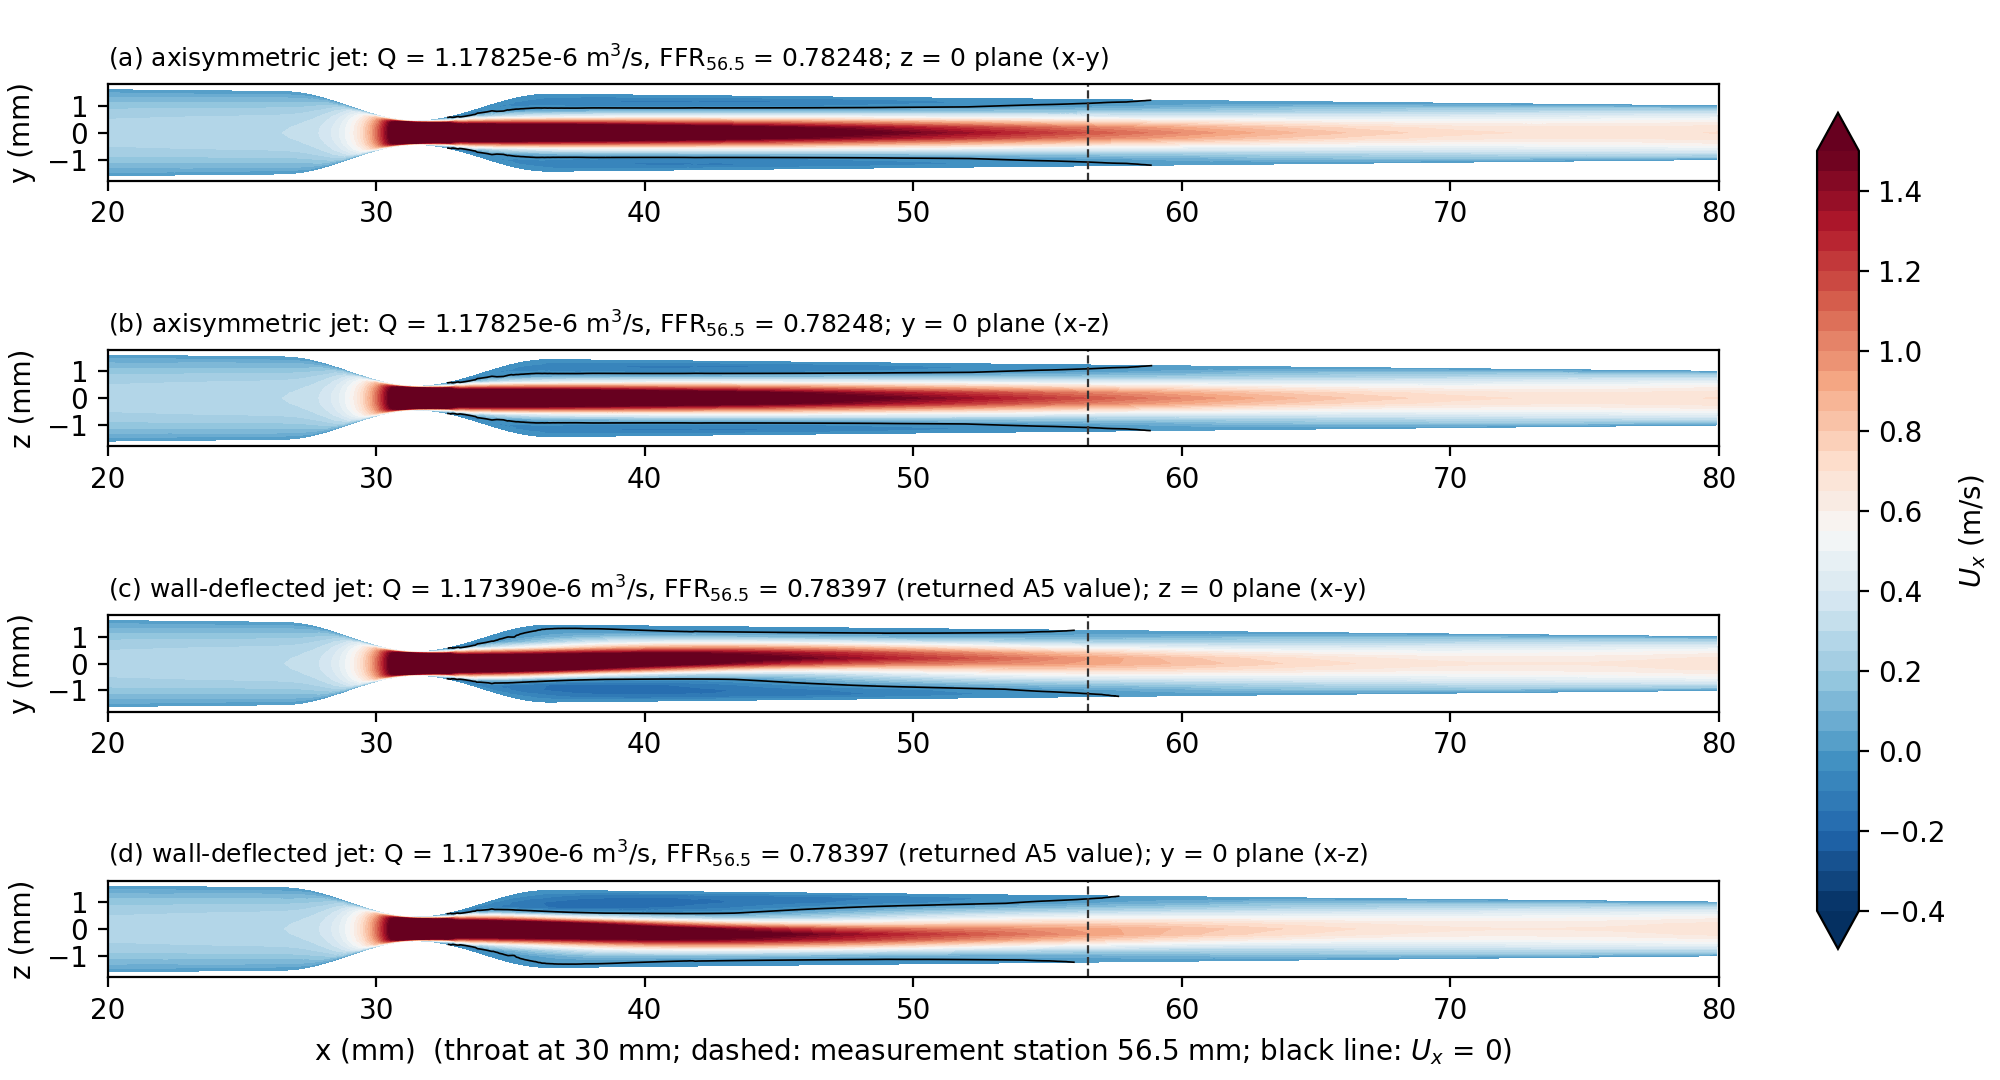
\includegraphics[width=\textwidth]{figures/cfd_sten70_two_states.png}
\caption[The two steady states of the Stage A sten70 case on the same mesh]{\label{fig:two-states}The two steady states of the Stage A sten70 case on the same mesh (the smoke-test mesh of 2026-10-01; state (c,d) obtained by restarting from the archived deflected solution): axial velocity on the two mid-planes, with the $U_x=0$ contour (black). (a,b) axisymmetric jet; (c,d) jet deflected towards $+y$, $-z$, the state of the returned A5 coarse value. Both are converged (flow band below $10^{-4}\%$ over 4000 iterations). Script \texttt{code\_\allowbreak{}from\_\allowbreak{}cfd/\allowbreak{}task\_\allowbreak{}0926/\allowbreak{}fig\_\allowbreak{}two\_\allowbreak{}states.py}; jet-offset diagnostic \texttt{jet\_offset.py}.}
\end{figure}

\textbf{Consequences for earlier results.} (i) \emph{A5 ladder} (\S\ref{sec:a5}): the archived coarse solution is on the deflected state (jet offset 85\,$\mu$m at $x=50$\,mm), the medium one close to axisymmetric (2.1\,$\mu$m) and the fine one weakly off-axis (7.2\,$\mu$m). The coarse level therefore belongs to a different state from the other two, which accounts for at least part of the non-monotone ladder; the verdict NOT ESTABLISHED stands. (ii) \emph{$U_{3D}$} (\S\ref{sec:u3d}): the fields of the five 3D levels were deleted after post-processing, so their state cannot be checked. The data are consistent with all levels being on the axisymmetric state (two independent zone families agree within $10^{-4}$ at each level, and the finest 3D level agrees with the axisymmetric wedge within $10^{-4}$), but this is not a verification, and on the coarse mesh the two states differ by 0.0015 in FFR, three times $U_{3D}$. $U_{3D}=0.00055$ is therefore a \textbf{provisional} scalar estimate until a jet-symmetry diagnostic exists for each level (a re-run with the fields kept). (iii) The scan-14 and scan-837 real-lumen cases are not axisymmetric and not covered by this finding; whether they admit more than one steady state was not tested.

\textbf{Change to the smoke test (fix 26, bug protocol: Opus~5.5, attempt 1; diagnosis and fix audited by GPT-5.6 Sol and Gemini~3.8 Flash).} The test now accepts either state and names it: PASS requires a complete run on the same mesh recipe and cell count (not mesh identity), an outlet flow within 0.1\% \emph{and} an FFR within 0.0005 of exactly one of the two states, and a steady final window (last 200 iterations: flow band $\leq0.01\%$, FFR band $\leq10^{-5}$). Only the deflected state reproduces the returned value; a pass on the axisymmetric state shows a correct install, not a reproduction of the returned number. The reference file holds both states with their provenance. Numerics, mesh recipe and iteration count are unchanged. The fix needed all three Opus attempts (post-fix audit round 1: GPT-5.6 Sol NOT READY, the state was identified by the flow alone; round 2: a test-environment and two documentation findings; round 3: READY from both auditors). \textbf{Result.} Two fresh runs of the installed test on 2026-10-01 (8 ranks, 3000 iterations, about 5 minutes each, 309--318\,s wall) landed one on each state: the first on the axisymmetric state (outlet flow $1.17825059\times10^{-6}$), the second on the deflected state, reproducing the returned A5 coarse value to $-3\times10^{-6}\%$ ($1.17392227\times10^{-6}$ against $1.17392231\times10^{-6}$); both PASS under the new rule, and the deflected reference entry now comes from that smoke run. Both runs had the same number of processor faces (2899), so the decomposition size alone does not select the state. \textbf{B3 is complete.}

\subsection{Task B2 of the 2026-09-26 work order: throughput of one 16-rank job against two 8-rank jobs}
\label{sec:b2}
\textbf{Set-up.} Scan-14 baseline, resistance mode (3{,}657{,}147 cells; the case rebuilt on 2026-10-01 from the deposited code, geometry and mesh identical to the returned records), 1600 iterations, no field writes; each job stopped by the B1 rule (first settled iteration 1229 in all three jobs). L16: one job, 16 ranks, one rank pinned per physical core; L8x2: two jobs side by side on disjoint sets of 8 physical cores. One replicate per layout, in the order L16 then L8x2 (2026-10-01, 08:15--12:50). The host was shared with another project of the study lead; at the study lead's request its processes were paused (SIGSTOP; 30 matching solver and queue processes holding 5.6\,GB of memory) and kept paused by a watcher, and resumed afterwards. The runner was extended for this (fix 27: admits only fully stopped foreign processes, re-checks them just before launch, records their fate and memory, and adds a host-level CPU measure calibrated beforehand by a rule fixed in advance, giving thresholds 0.48/1.62 cores); the change needed three Opus~5.5 and two Fable~5.1 attempts and four audit rounds (GPT-5.6 Sol and Gemini~3.8 Flash; final verdicts READY WITH CONDITIONS from both). The Windows pre-check was overridden (the terminal process used about 0.5 core), so the best attainable label was CONDITIONALLY COMPARABLE.

\textbf{Result.} L16 reached the settle point after 4143\,s (0.869 solves per hour; an earlier uncontended 16-rank solve of the same case took 4067\,s, $+1.9\%$); the two L8x2 jobs after 8834 and 8895\,s (together 0.812 solves per hour; 0.809 if paired by the slower job). L8x2/L16 $=0.935$: on this host one 16-rank job gives about 7\% more solves per hour than two 8-rank jobs. \textbf{Status: both layouts are INVALID under the strict isolation rule and the ratio is NOT CLAIMED.} The non-owned CPU was small on average (per-process mean 0.039 and 0.045 core, host-level 0.070 and 0.077 core, i.e.\ below 0.5\% of the 16 cores) but had short peaks above the 1-core limit: in L16 the coordinating Claude session (1.15 cores), in L8x2 the operating system's daily package update (\texttt{apt}/\texttt{unattended-upgrades}, \texttt{systemd} up to 3.2 cores) and an automatic update of a command-line tool (\texttt{npm install}). All 30 paused processes stayed paused through both layouts, no new foreign job appeared, swap was not used, and the minimum available memory was 17.4 and 12.7\,GB. The 7\% figure is therefore reported as indicative only; a claim needs a replicate on a host with automatic updates disabled and no interactive session, ideally in both orders.

\subsection{Task A of the 2026-10-03 work order: the D7 sensitivity test (variants A1 and A2, control A0)}
\label{sec:taskA}
\textbf{Question and rule (pre-registered before any solve, \texttt{TASK\_A\_DESIGN.md}).} Decision D7 makes Gate M1 a pass for the lesion cases only through a declared deviation backed by a sensitivity test: the scan-14 baseline is re-meshed with the throat zone at 12.5\,$\mu$m instead of 25\,$\mu$m and solved in resistance mode with the production template of Task~C (bounded probe monitors, fields kept, 16 ranks and 3000 iterations as the returned solve). The acceptance statistic is the section-averaged pressure at the measurement probe p011, $p/P_\text{aorta}$ on the reconstructed iteration-3000 fields by the same connected-section method as the returned value (0.8697575): a variant passes with deviations if the difference is below $U_{3D}=0.00055$ (provisional), otherwise M1 fails for the lesion cases and the fallback of section~9 of the work order opens. No surface repair is allowed. Variant A1 is the plain 12.5\,$\mu$m zone ($\pm4$\,mm); A2 shifts the zone interfaces by 1\,mm ($-3$ to $+5$\,mm), as in the U3D ladder, because A1 still has flagged face-tets within 2\,mm of the throat. The control A0 re-solves the regenerated production mesh (25\,$\mu$m) with the same template: it shows whether a regenerated mesh reproduces the returned value, i.e. whether a shift can be attributed to the resolution.

\begin{table}[H]
\centering
\caption{\label{tab:taskA}Task A: scan-14 baseline, resistance mode, 16 ranks, 3000 iterations. $\Delta$ = $p/P_\text{aorta}$ minus the returned baseline (25\,$\mu$m zone) at the same probe.}
\small
\begin{tabular}{lrrrr}
\toprule
 & returned (25\,$\mu$m) & A0 (control, 25\,$\mu$m) & A1 (12.5\,$\mu$m) & A2 (12.5\,$\mu$m, shifted) \\
\midrule
cells & 3{,}657{,}147 & 3{,}657{,}147 & 6{,}241{,}438 & 8{,}308{,}794 \\
upstream probe p003 ($-4.7$\,mm): $\Delta$ & --- & $0.00000$ & $-0.00001$ & $-0.00001$ \\
throat plane p004: $\Delta$ & --- & $0.00000$ & $+0.00099$ & $+0.00097$ \\
5\,mm distal p005: $\Delta$ & --- & $0.00000$ & $+0.00195$ & $+0.00200$ \\
measurement probe p011: $p/P_\text{aorta}$ & 0.86976 & 0.86976 & 0.87165 & 0.87183 \\
\textbf{$\Delta$ at p011} & --- & $\mathbf{0.0000000}$ & $\mathbf{+0.00189}$ & $\mathbf{+0.00207}$ \\
$\Delta$ at the end of the tree (p023, 90\,mm distal) & --- & $0.00000$ & $+0.00188$ & $+0.00206$ \\
outlet flows out\_160 / out\_600 & --- & $0.00\%$ & $+0.24\%$ / $+0.24\%$ & $+0.25\%$ / $+0.25\%$ \\
other four outlets & --- & $0.00\%$ & $<0.003\%$ & $<0.001\%$ \\
strict \texttt{checkMesh}: nearest flagged entity to the throat / to p011 (mm) & 1.43 / 2.55 & 1.43 / 2.55 & 0.70 / 2.55 & 0.70 / 2.55 \\
D4 & FAIL & FAIL & FAIL & FAIL \\
strict residual criterion (final $U_y$ residual $<10^{-5}$) & --- & met & met & $1.08\times10^{-5}$: not met \\
B1 SETTLED rule on \texttt{measurementP}: first settled iteration & --- & 1421 & 2193 & 2614 \\
\bottomrule
\end{tabular}
\end{table}

\textbf{Result.} Neither variant meets the acceptance criterion: $|\Delta|$ at p011 is $0.00189$ (A1) and $0.00207$ (A2), 3.4 and 3.8 times $U_{3D}$ (22.7 and 24.9\,Pa, 0.17 and 0.19\,mmHg). Upstream of the lesion the two variants differ from the returned baseline by at most $1.5\times10^{-5}$; the difference arises across the throat and then varies by less than $10^{-4}$ along the next 90\,mm of the LAD (A1: $+0.00195$ five mm distal, $+0.00188$ at the most distal probe; A2: $+0.00200$ to $+0.00209$; Fig.~\ref{fig:taskA-profile}), i.e. the finer throat zone changes the added loss across the lesion by $0.0019$ to $0.0021$, and the rest of the tree hardly at all. The two 12.5\,$\mu$m variants agree with each other to $0.00018$ (below $U_{3D}$), so this is not an artefact of where the refined zone ends (the finer zone lowers the loss across the lesion; the sign is opposite to the straight-tube ladder of the U3D study); the outlet flows change by at most $0.25\%$. \textbf{Control A0.} The regenerated production mesh (25\,$\mu$m, 3{,}657{,}147 cells, regenerated by cfMesh with the new template and the bounded probe monitors) reproduces the returned baseline to seven digits at p011 ($0.8697575$, $\Delta=0.0000000$) and at every probe and outlet; so the pipeline, the template change and a regenerated mesh do not move the result, and the shift of A1 and A2 is a genuine effect of the finer throat zone: on this lesion (80\%DS, throat radius 0.28\,mm) the measurement-probe value shows a 25-to-12.5\,$\mu$m throat-zone resolution sensitivity of 0.0019 to 0.0021 in $p/P_\text{aorta}$ (0.2\% of the value, 3.4 to 3.8 times $U_{3D}$ of the straight tube); no finer level was run, so this is a sensitivity, not an estimate of the asymptotic discretisation error. By the rule as written M1 fails for the lesion cases and the fallback discussion opens (not decided here). The strict \texttt{checkMesh} flag nearest to the throat (face tets, 0.70\,mm) is the same entity in both variants, so it is not removed by either zone choice; nothing was repaired. A2 is marked not converged in the returns only because the final $U_y$ residual ($1.08\times10^{-5}$) exceeds the strict $10^{-5}$ threshold; its inlet pressure varies by 0.0004\,Pa over the last 500 iterations and the monitors settle at iteration 2614.

\textbf{Flow state.} The pre-registered curved-lumen diagnostic (flux-weighted velocity centroid offset over the section radius every 1\,mm from the throat to p011) is INDETERMINATE for A1 against A2: the profile is not available at the section 23--24\,mm distal to the throat (invalid section), and the rule requires the full profile. For information only, over the 28 of 30 stations valid in both, A1 and A2 differ by up to 0.22 radii (at 9\,mm distal to the throat; tolerance 0.03) while the FFR criterion agrees ($0.00018<0.00055$); A0 against A1 differ by at most 0.019 radii (at 5\,mm, within the tolerance) although their FFR differs by $0.0019$, i.e. the FFR shift is not accompanied by a change of the jet-centroid profile. No claim of bistability is made: the two-state behaviour of the straight sten70 case is not assumed for this lumen, and a two-state restart demonstration is not part of this task.

\begin{figure}[H]
\centering
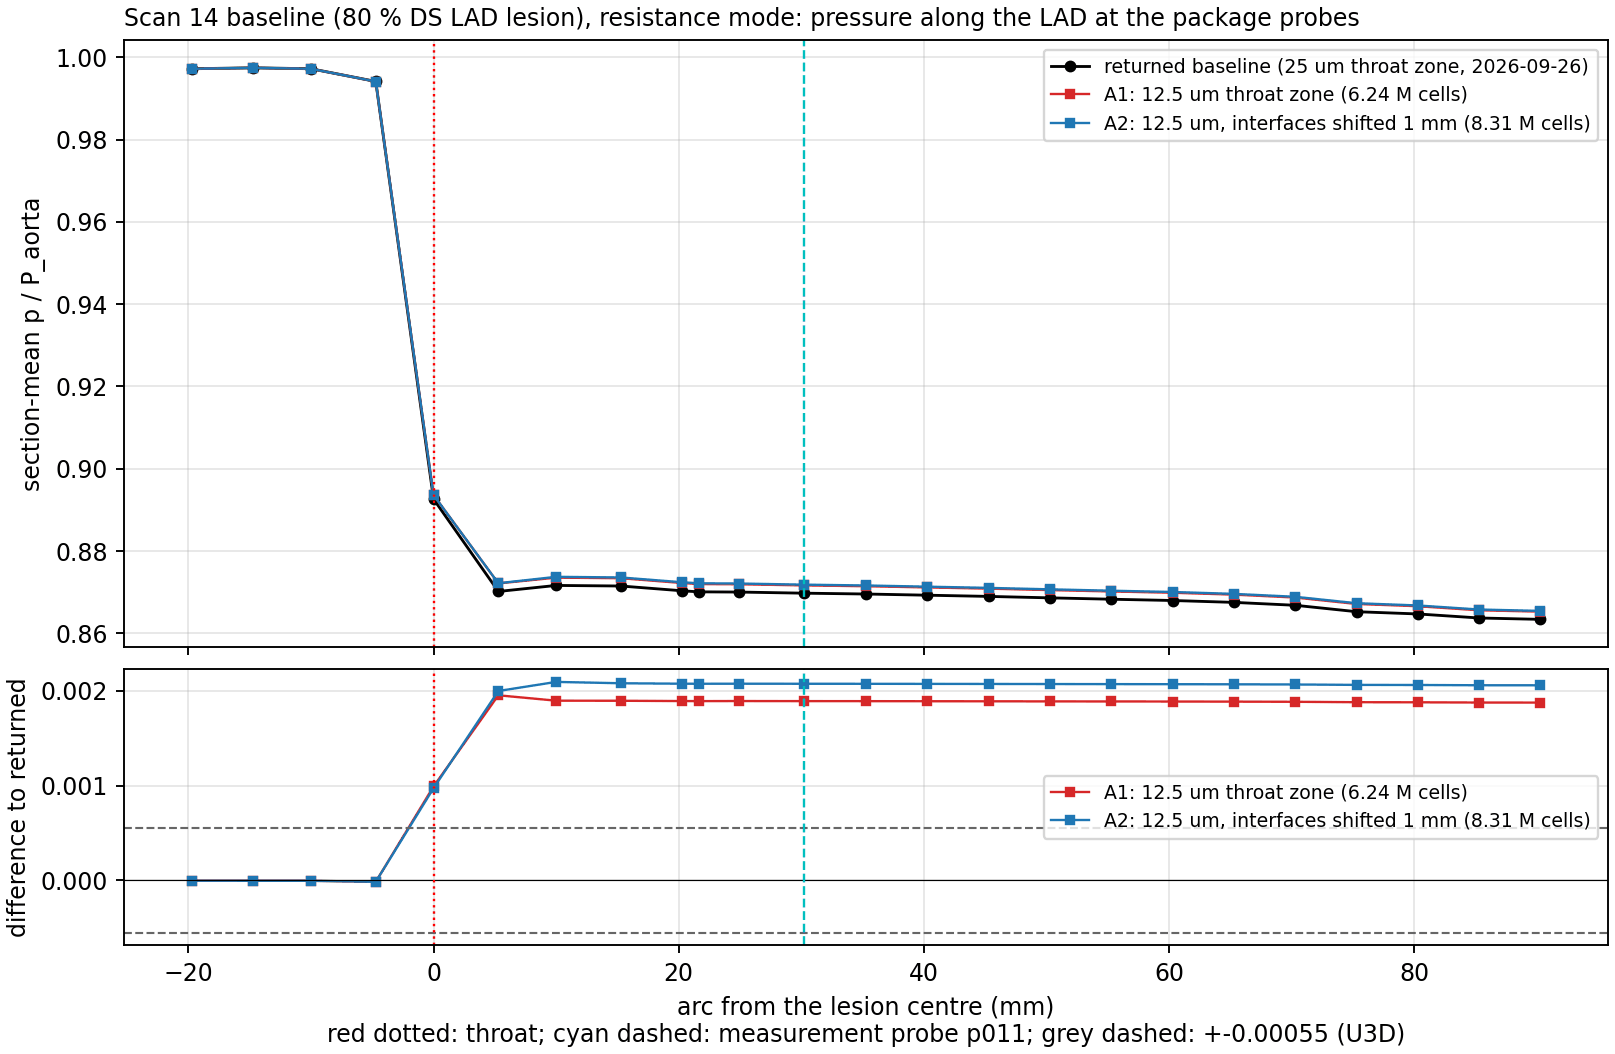
\includegraphics[width=\textwidth]{figures/cfd_taskA_profile.png}
\caption[Task A: pressure along the LAD against the returned baseline]{\label{fig:taskA-profile}Task A: section-mean $p/P_\text{aorta}$ at the package probes along the LAD for the returned baseline (25\,$\mu$m), the control A0 (regenerated 25\,$\mu$m), A1 and A2 (12.5\,$\mu$m), and the differences (lower panel; dashed: $\pm U_{3D}$). A0 coincides with the returned baseline; A1 and A2 differ from the baseline by at most $1.5\times10^{-5}$ upstream of the lesion and are offset by about $+0.002$ downstream.}
\end{figure}

\begin{figure}[H]
\centering
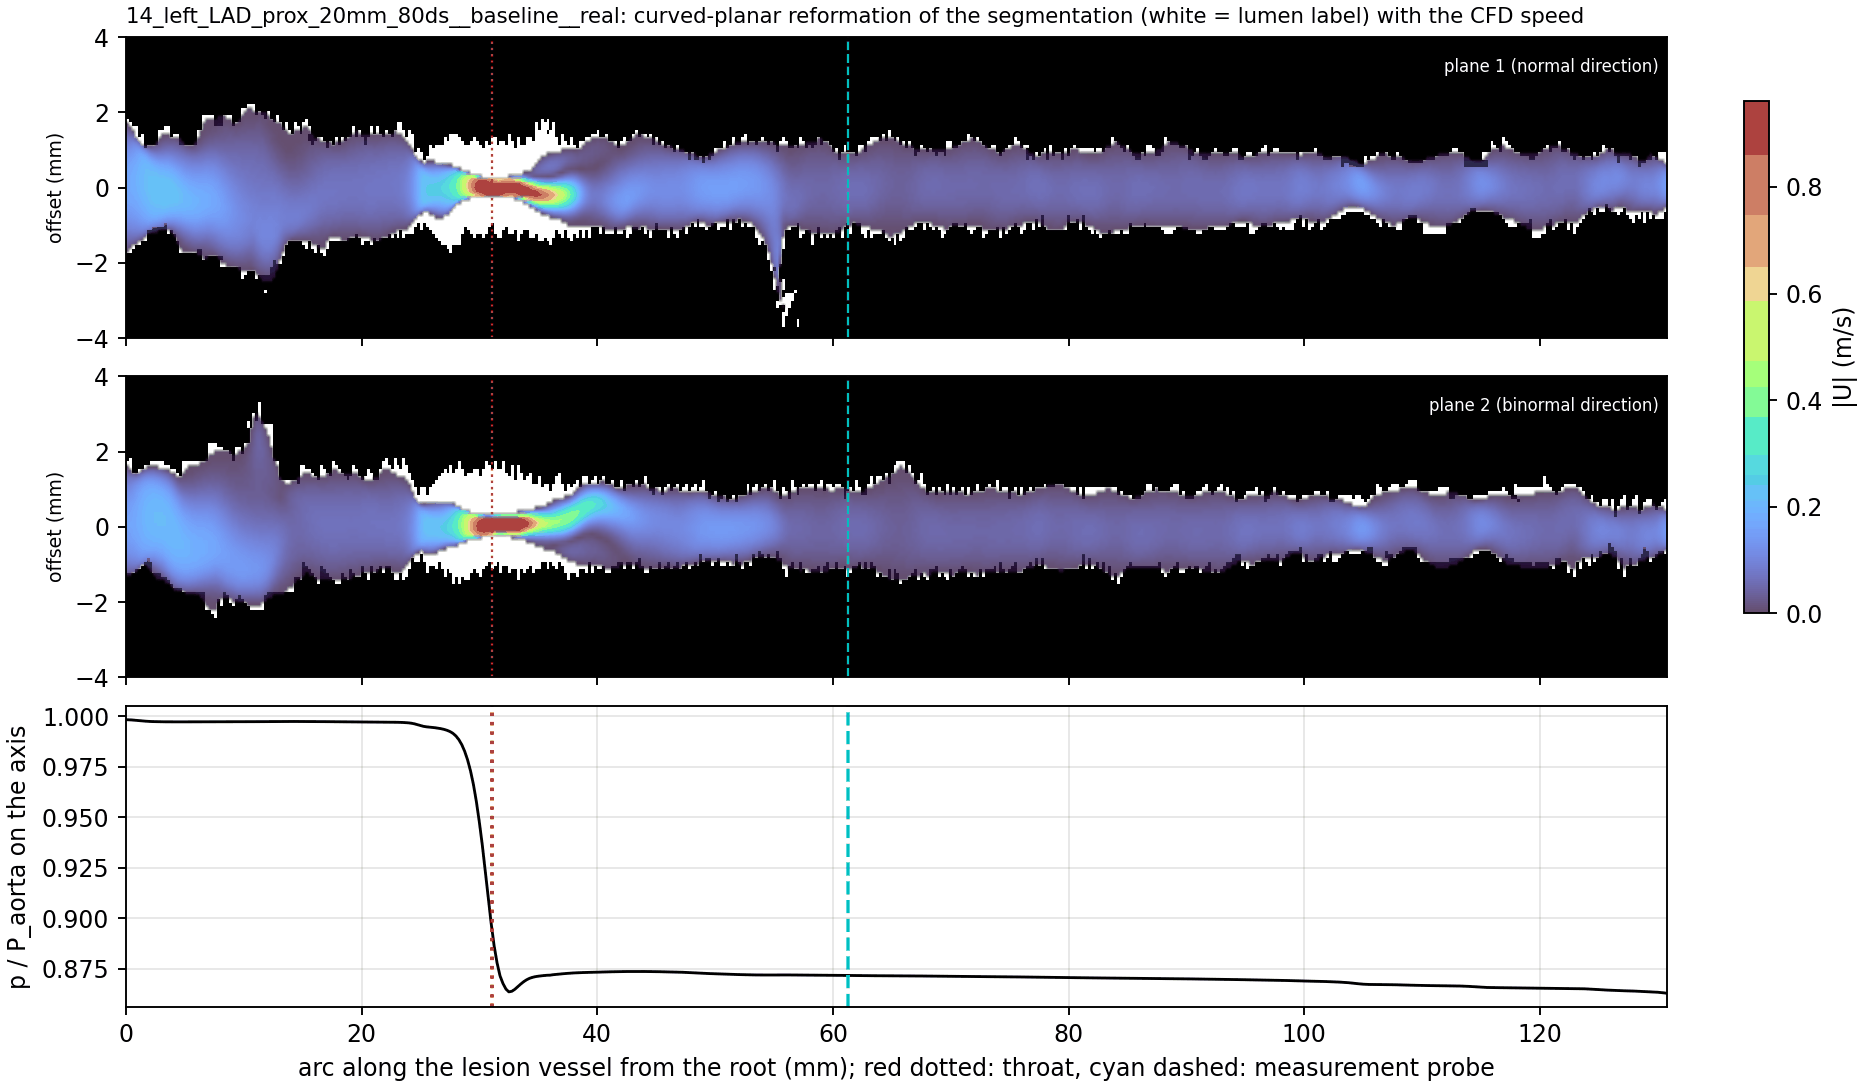
\includegraphics[width=\textwidth]{figures/img_taskA_A1_cpr_cfd.png}
\caption[Task A, variant A1: curved-planar reformation of the segmentation with the CFD speed]{\label{fig:taskA-cpr}Imaging part, variant A1: curved-planar reformation of the unmodified ImageCAS-X lumen label (white) along the lesion vessel in two orthogonal planes with the CFD speed $|U|$ in the CFD domain, and $p/P_\text{aorta}$ on the axis (bottom). The synthetic 80\% stenosis exists only in the CFD surface: the label is wider than the CFD lumen at the throat (white margins). Red dotted: throat; cyan dashed: measurement probe p011. Script \texttt{code\_\allowbreak{}from\_\allowbreak{}cfd/\allowbreak{}task\_\allowbreak{}1003/\allowbreak{}viz/\allowbreak{}viz\_\allowbreak{}imaging.py}.}
\end{figure}

\begin{figure}[H]
\centering
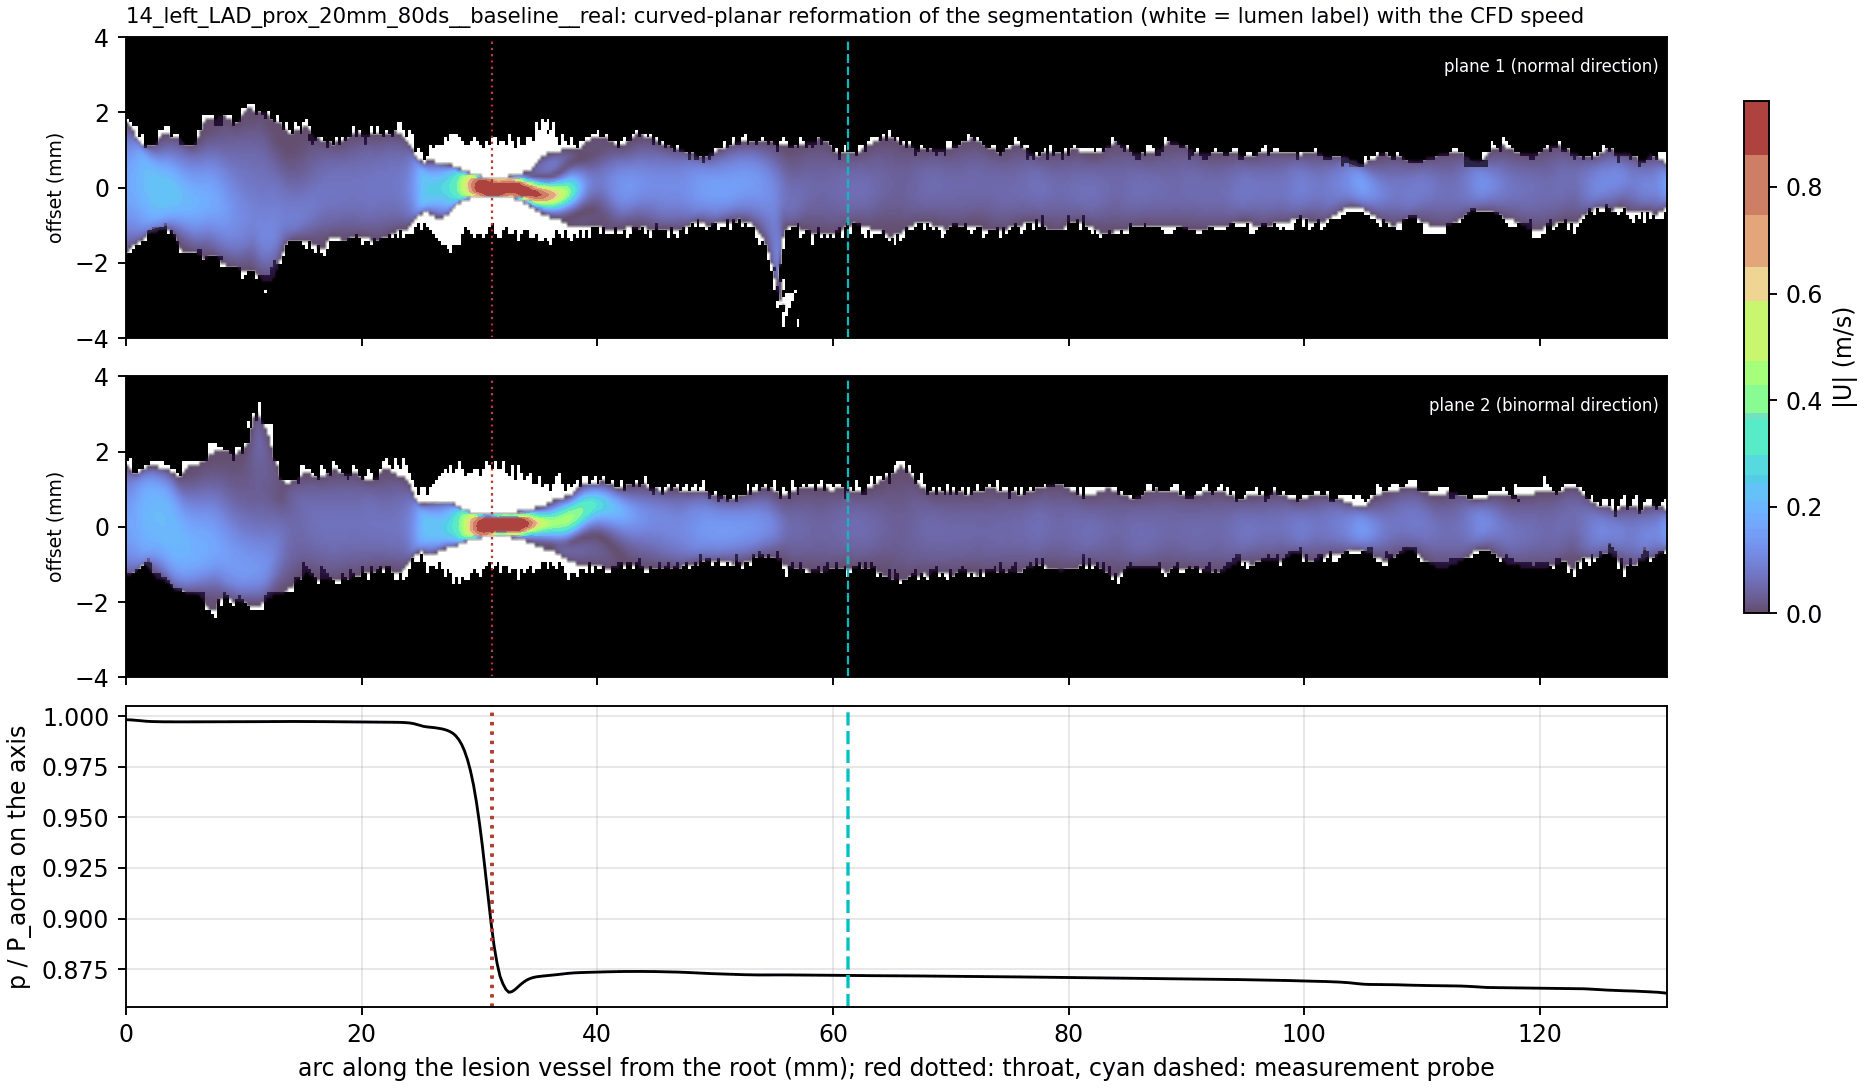
\includegraphics[width=\textwidth]{figures/img_taskA_A2_cpr_cfd.png}
\caption[Task A, variant A2: curved-planar reformation of the segmentation with the CFD speed]{\label{fig:taskA-cpr2}Variant A2 (zone interfaces shifted by 1\,mm), same layout as Fig.~\ref{fig:taskA-cpr}.}
\end{figure}

\begin{figure}[H]
\centering
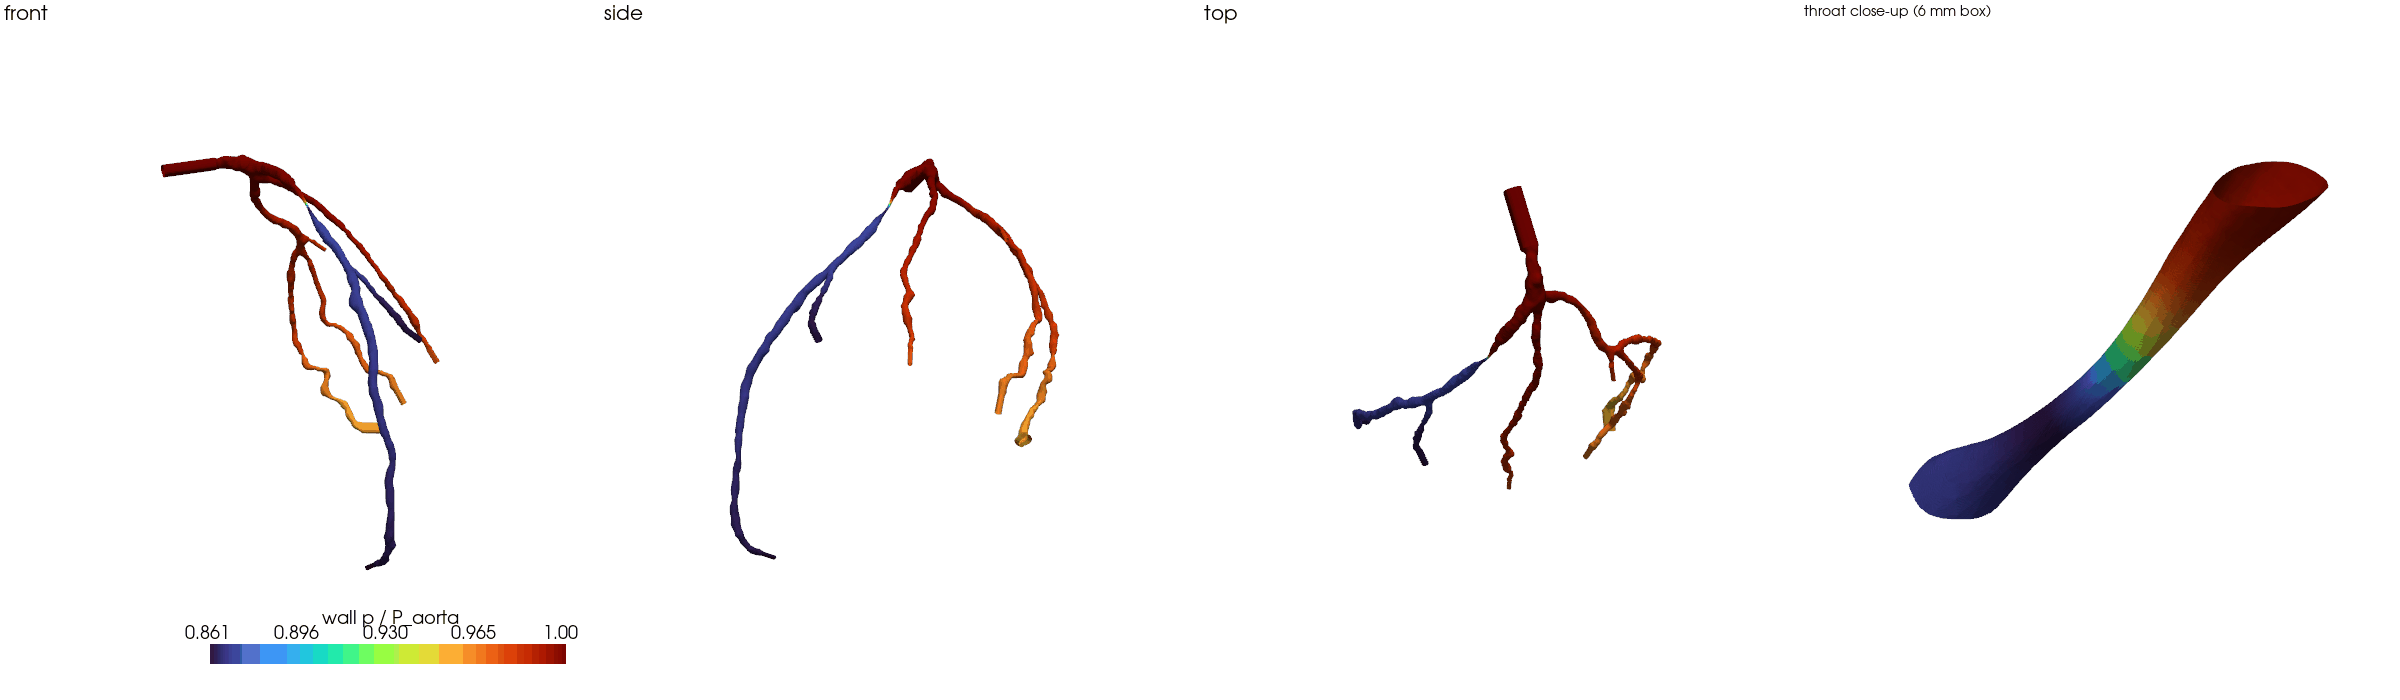
\includegraphics[width=\textwidth]{figures/cfd_taskA_A1_wall_pressure.png}
\caption[Task A, variant A1: wall pressure of the left coronary tree]{\label{fig:taskA-wall}Variant A1: wall pressure $p/P_\text{aorta}$ of the whole left coronary tree in three views and a close-up of the 6\,mm around the throat (same colour scale).}
\end{figure}

\begin{figure}[H]
\centering
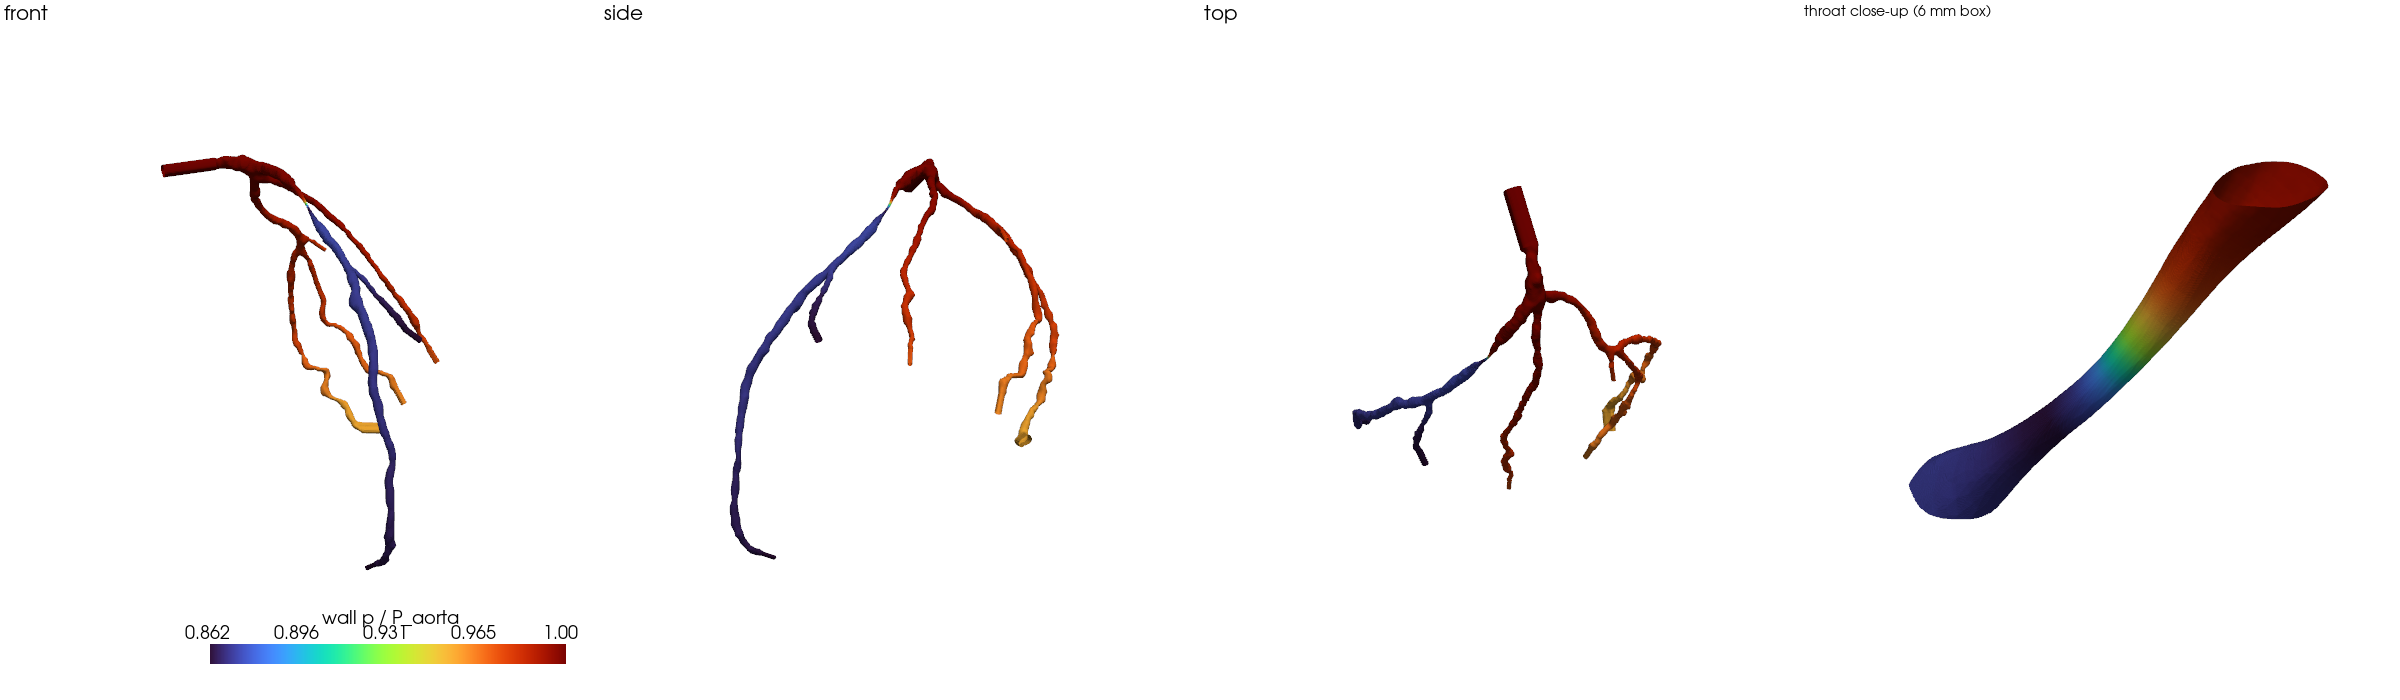
\includegraphics[width=\textwidth]{figures/cfd_taskA_A2_wall_pressure.png}
\caption[Task A, variant A2: wall pressure of the left coronary tree]{\label{fig:taskA-wall2}Variant A2 (zone interfaces shifted by 1\,mm): wall pressure, same layout and colour scale as Fig.~\ref{fig:taskA-wall}.}
\end{figure}

\subsection{Task B of the 2026-10-03 work order: making $U_{3D}$ final (levels re-run so far)}
\label{sec:taskB}
\textbf{Procedure} (rule of \texttt{U3D\_CHECK\_DESIGN.md}, dated extension of 2026-10-03, written before any of these runs). The remaining levels of the sten70 ladder are re-run with the fields kept, at 8 ranks on regenerated meshes with the original cell counts and budgets, one after the other (S25B, S12A, S12B); each run is classified by its own job script: \emph{axisymmetric} if it is SETTLED, the jet centroid is within 10\,$\mu$m of the axis at $x=50$ and 56.5\,mm and the FFR equals the original within $10^{-4}$ (the original level is then verified on the same state), \emph{deflected} if it is SETTLED and the offset is 30\,$\mu$m or more at either station, \emph{symmetric but FFR differs} if it is SETTLED with offsets of at most 10\,$\mu$m but $|\Delta\text{FFR}|>10^{-4}$ (a mesh-realisation effect, no conclusion on the original state), and inconclusive otherwise (always if not SETTLED). If all five levels are axisymmetric, $U_{3D}$ becomes final; if any is deflected the ladder is reported per state.

\begin{table}[H]
\centering
\caption{\label{tab:taskB}Jet-state check of the U3D levels (re-runs with fields kept; the first two on 2026-10-02 with the earlier script, S25B on 2026-10-04 with the audited job script).}
\small
\begin{tabular}{lrrrrrl}
\toprule
level & cells & iterations & FFR re-run & FFR original & offset 50 / 56.5\,mm ($\mu$m) & verdict \\
\midrule
S50 & 2{,}687{,}640 & 3000 & 0.793363 & 0.793362 & 0.0 / 0.4 & axisymmetric \\
S25A & 3{,}194{,}196 & 4000 & 0.791103 & 0.791103 & 0.0 / 0.1 & axisymmetric \\
S25B & 3{,}299{,}948 & 4000 & 0.791197 & 0.791197 & 0.0 / 0.1 & axisymmetric \\
S12A & 6{,}739{,}168 & 6000 & 0.790308 & 0.790308 & 0.0 / 0.0 & axisymmetric \\
S12B & 7{,}649{,}800 & 3000 & 0.790418 & 0.790418 & 1.2 / 2.3 & axisymmetric \\
\bottomrule
\end{tabular}
\end{table}

\textbf{Result so far.} S25B reproduces the original value to $3\times10^{-8}$ (last-100 band $6\times10^{-8}$, drift over the final 500 iterations $5\times10^{-9}$) with an axisymmetric jet, so rule (a) holds: the original S25B, the coarse level of the shifted-zone family, was on the axisymmetric state. With S50, S25A and S25B verified, both zone families are verified at their two coarser levels; S12A (6.7 million cells, 6000 iterations) reproduces the original value to $3\times10^{-7}$ (last-100 band $2\times10^{-8}$) with an axisymmetric jet, so rule (a) holds for it too; S12B (7.6 million cells, 3000 iterations) likewise reproduces the original value to $4\times10^{-7}$ (last-100 band $5\times10^{-8}$, offsets 1.2 and 2.3\,$\mu$m) with an axisymmetric jet. All five levels are therefore verified on the axisymmetric state and $U_{3D}=0.00055$ is made final under decision D9 (the verification rests on the FFR reproduction and the jet state of the re-runs, not on decomposition identity). The re-runs use 8 ranks and regenerated meshes (the originals 16 ranks on the original meshes): the evidence about the original state is the FFR reproduction within $10^{-4}$ together with the jet state, not decomposition identity. Fig.~\ref{fig:taskB-states} shows the axisymmetric jet of S50 and S25B in the two mid-planes.

\begin{figure}[H]
\centering
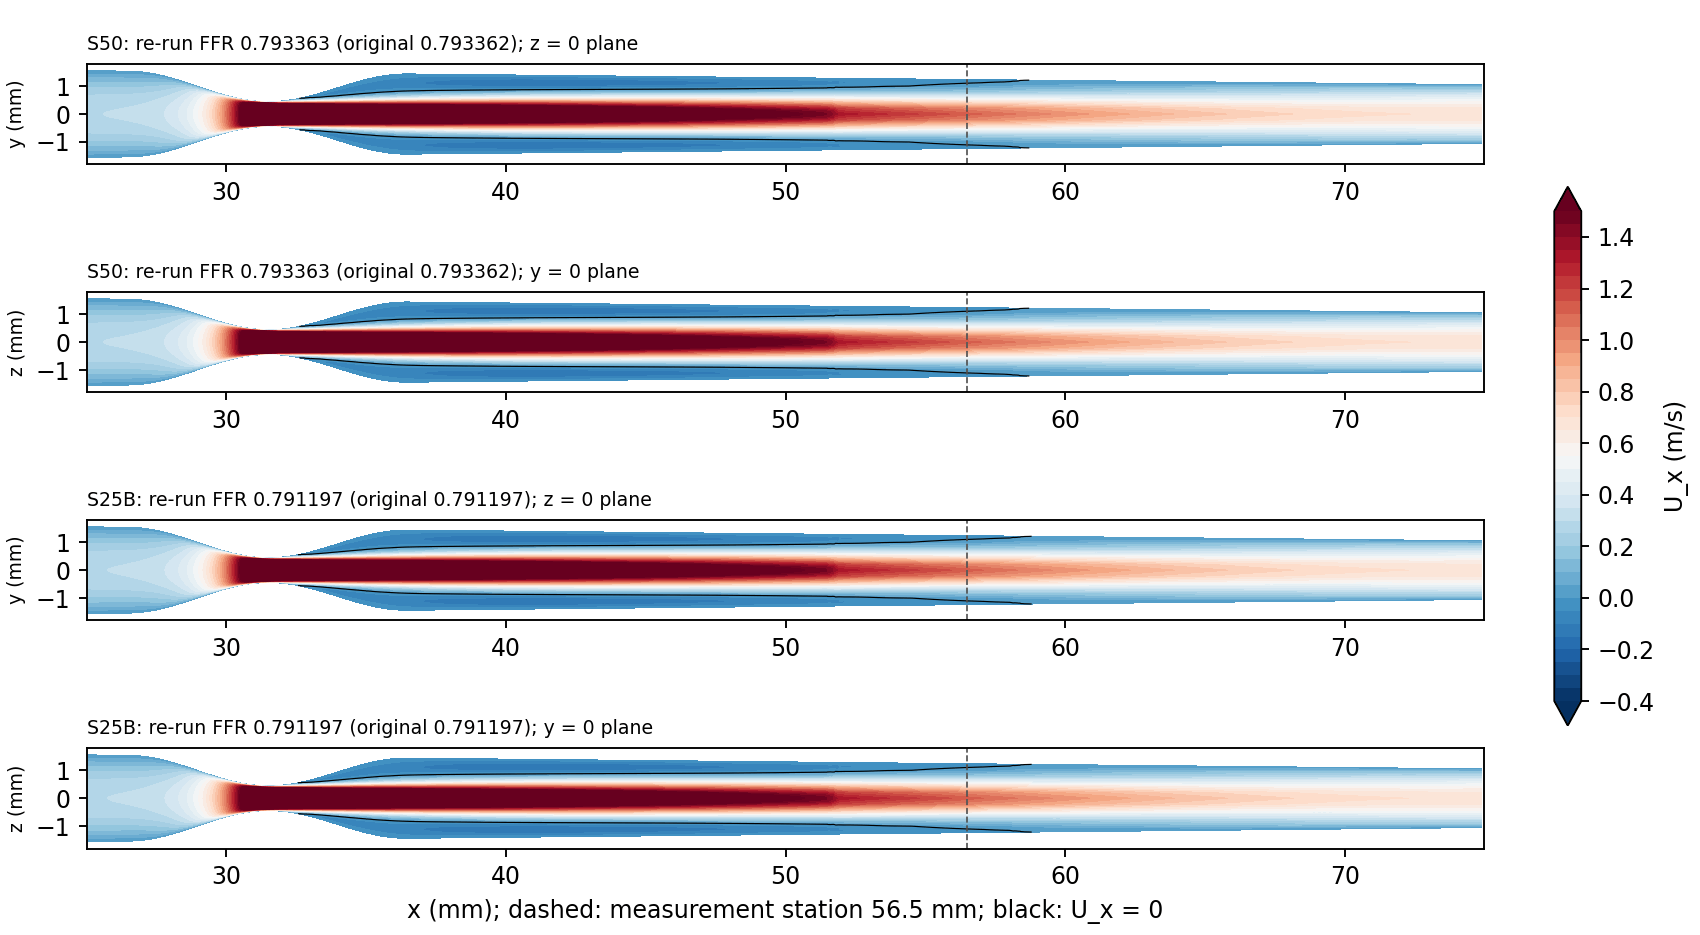
\includegraphics[width=\textwidth]{figures/cfd_taskB_u3d_states.png}
\caption[Task B: axial velocity of the re-run U3D levels S50 and S25B]{\label{fig:taskB-states}Task B: axial velocity on the two mid-planes of the re-run levels S50 and S25B (throat at 30\,mm, $U_x=0$ contour in black, dashed: measurement station 56.5\,mm). Both jets are axisymmetric and the FFR equals the original value (to $10^{-6}$ and $3\times10^{-8}$). Script \texttt{code\_\allowbreak{}from\_\allowbreak{}cfd/\allowbreak{}task\_\allowbreak{}1003/\allowbreak{}viz/\allowbreak{}viz\_\allowbreak{}u3d\_\allowbreak{}states.py}.}
\end{figure}

%%P5_BEGIN
\subsection{Task P5 of the 2026-10-03 work order: five-case baseline pilot (results so far)}
\label{sec:p5}
\textbf{Design.} Five new cohort baselines (scans 138, 69, 473, 272, 139; selected by the analysis side by a fixed rule), baseline geometry only, one resistance-mode solve each with the production recipe (25\,$\mu$m throat zone, 4 boundary layers, bounded probe monitors of Task~C, 3000 iterations, fields kept), built by the generalised pipeline (\texttt{code\_\allowbreak{}from\_\allowbreak{}cfd/\allowbreak{}task\_\allowbreak{}1003/\allowbreak{}p5\_\allowbreak{}builders}; its regression on scan 14 reproduces the STL byte for byte and the mesh cell count). Gates are reported, not repaired: a case that fails a gate is solved and returned flagged. The solves ran concurrently with other jobs (up to 32 MPI ranks on the 16 physical cores, at the study lead's request, against the 16-rank cap of the work order of 2026-09-24 and a pre-run audit condition), so the wall-clock columns of the returns are contended and must not be used as cost figures. \textbf{Execution-order deviation:} the work order asked for the order 138, 69, 473, 272, 139; scan 473 was started (2026-10-04 13:58, in the second scheduler lane) while 69 was still running, and 139 (2026-10-05 09:18) before 272 (10:44). The solves are independent steady computations, so the order does not change any result, but the prescribed order was not kept. No 0D prediction is available or used for these cohort scans; the 3D values below are for the analysis side to compare.

\begin{table}[H]
\centering
\caption{\label{tab:p5}P5 cases: lesion vessel, length / diameter stenosis (mm / \%), cells, convergence verdict, throat Reynolds number, $p/P_\text{aorta}$ at the measurement probe used, and the machine-readable gate flags (D2: relative throat gate; D3: a self-intersection of mask origin, accepted only with conditions; D4: a strict \texttt{checkMesh} failure within 2\,mm of the throat or the measurement probe).}
\small
\resizebox{\textwidth}{!}{\begin{tabular}{llrrlrll}
\toprule
scan & vessel & L / DS & cells & verdict & Re$_\text{throat}$ & $p/P_\text{aorta}$ at measurement & flags \\
\midrule
138 & LAD & 20 / 70 & 4{,}941{,}176 & converged & 264 & 0.87816 (p010) & D3\_FAIL, D4\_FAIL, CHECKMESH\_STANDARD\_FAIL \\
69 & LCx & 20 / 65 & 4{,}218{,}023 & converged & 366 & 0.86960 (p012) & LESION\_PURITY\_GATE\_FAIL, POSITIVE\_CONTROL\_UNDETECTED \\
473 & LCx & 20 / 60 & 5{,}487{,}673 & converged & 400 & 0.88333 (p011\_reloc; package p011, failed section rule: 0.88685) & D2\_RELATIVE\_THROAT\_GATE\_FAIL, D3\_FAIL, D4\_FAIL, MEASUREMENT\_PROBE\_RELOCATED \\
272 & RCA & 10 / 65 & 7{,}639{,}018 & converged (truncated domain) & 320 & 0.93861 (p009) & SELF\_INTERSECTION, D3\_FAIL, D4\_FAIL, OUTLET\_LOST\_IN\_MESH (out\_396) \\
139 & RCA & 10 / 70 & 4{,}138{,}185 & converged & 236 & 0.85674 (p009) & D2\_RELATIVE\_THROAT\_GATE\_FAIL, D3\_FAIL, D4\_FAIL \\
\bottomrule
\end{tabular}}
\end{table}

\begin{figure}[H]
\centering
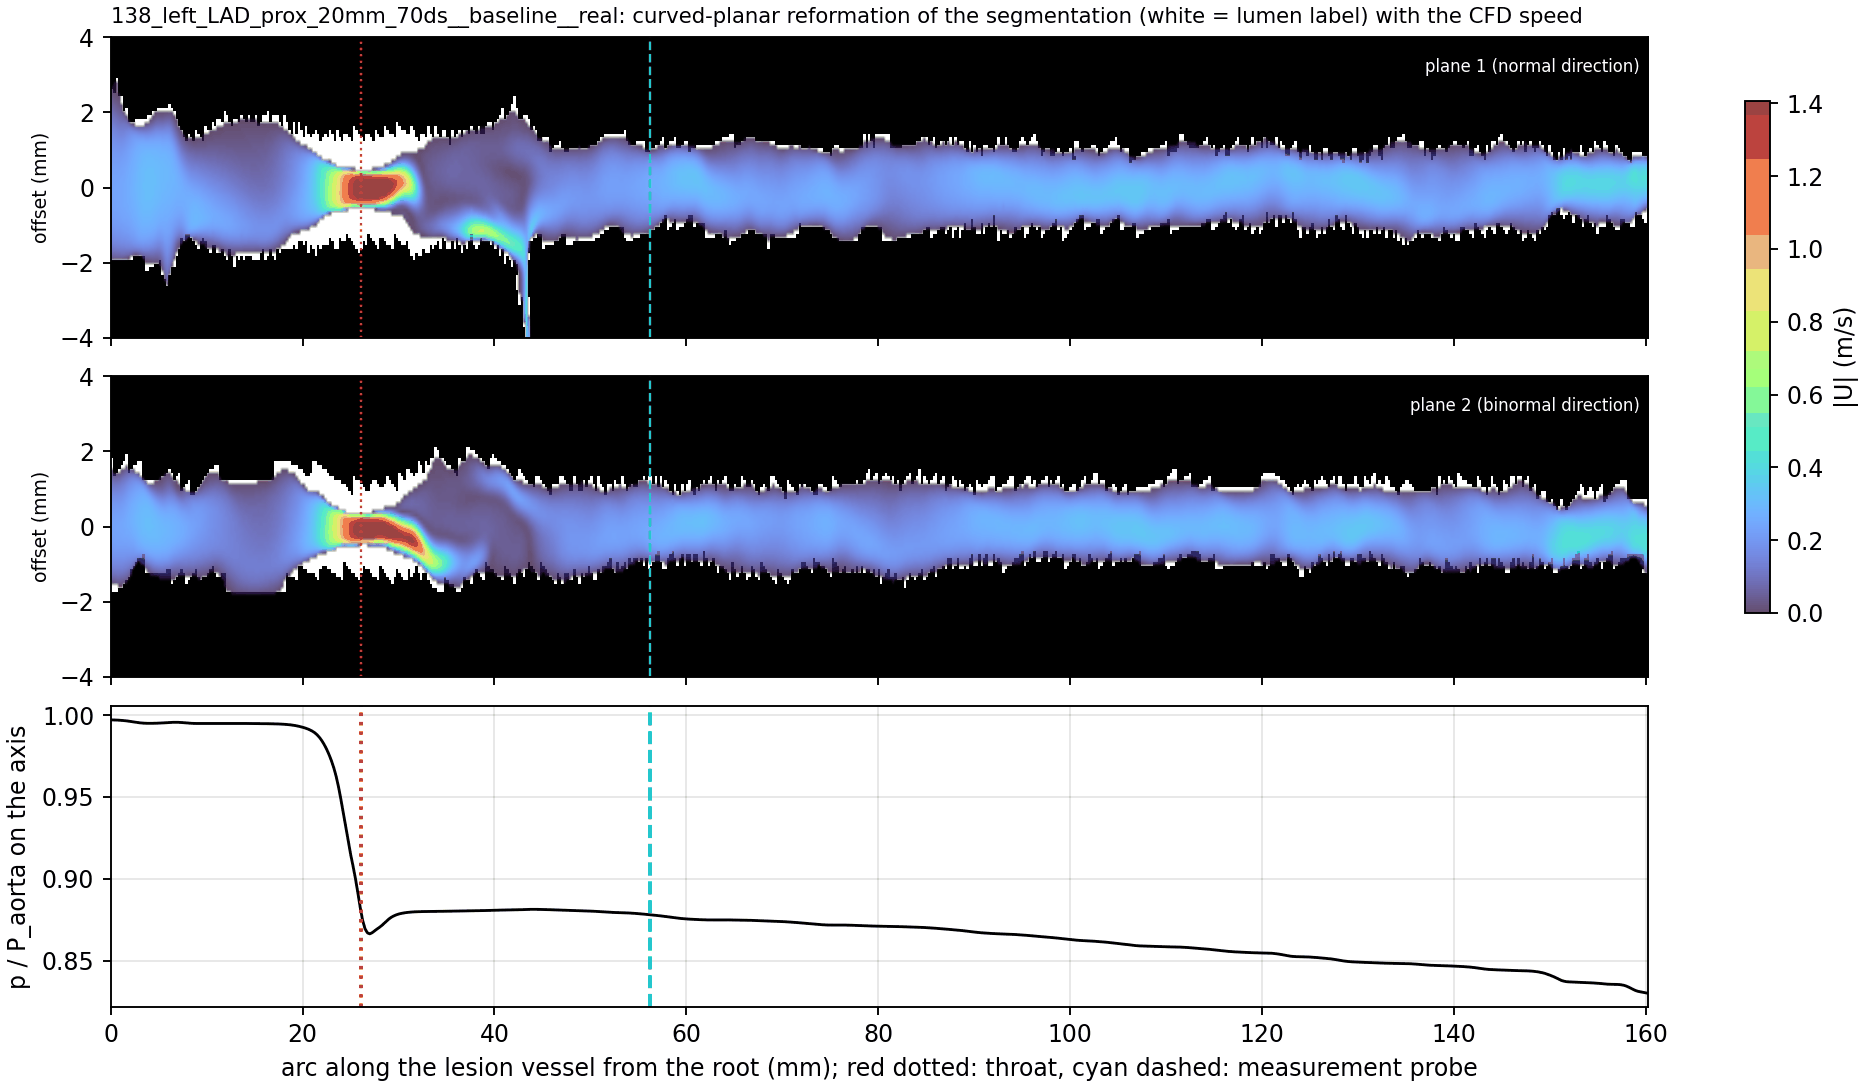
\includegraphics[width=\textwidth]{figures/cfd_p5_138_cpr_cfd.png}
\caption[P5 scan 138: segmentation reformation with the CFD speed]{P5 scan 138 (LAD, 20\,mm, 70\%DS): curved-planar reformation of the unmodified lumen label (white) in two orthogonal planes with the CFD speed $|U|$ in the CFD domain (the synthetic stenosis exists only in the CFD surface), and $p/P_\text{aorta}$ on the axis (bottom); red dotted: throat, cyan dashed: measurement probe.}
\end{figure}
\begin{figure}[H]
\centering
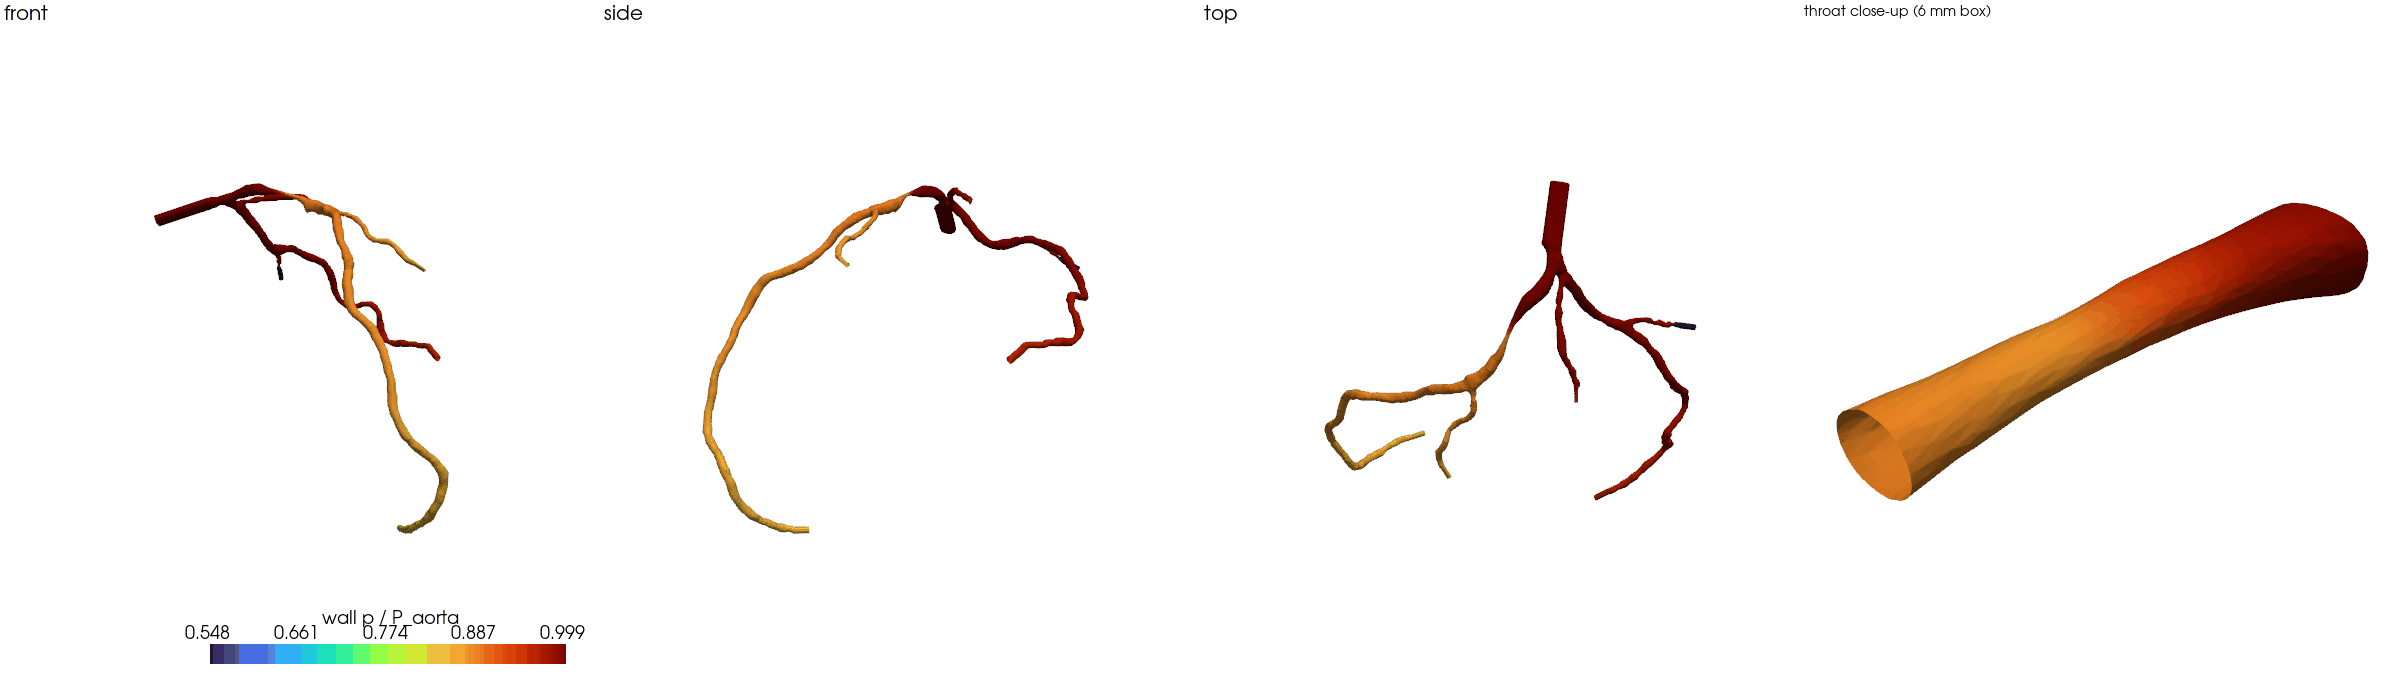
\includegraphics[width=\textwidth]{figures/cfd_p5_138_wall.png}
\caption[P5 scan 138: wall pressure]{P5 scan 138: wall pressure $p/P_\text{aorta}$ of the tree in three views and the 6\,mm around the throat.}
\end{figure}

\begin{figure}[H]
\centering
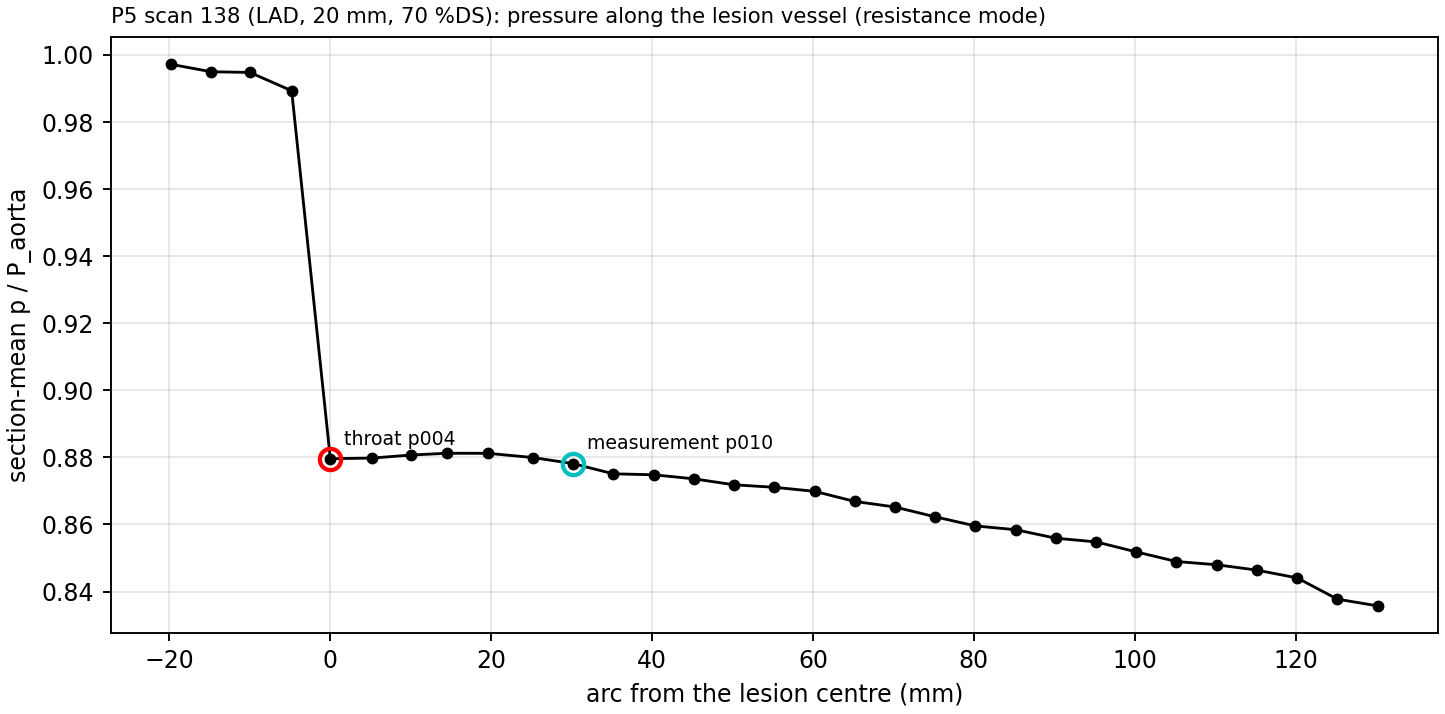
\includegraphics[width=0.85\textwidth]{figures/cfd_p5_138_profile.png}
\caption[P5 scan 138: pressure along the lesion vessel]{P5 scan 138: section-mean $p/P_\text{aorta}$ at the package probes along the lesion vessel (resistance mode), with the throat and measurement probes marked.}
\end{figure}


\begin{figure}[H]
\centering
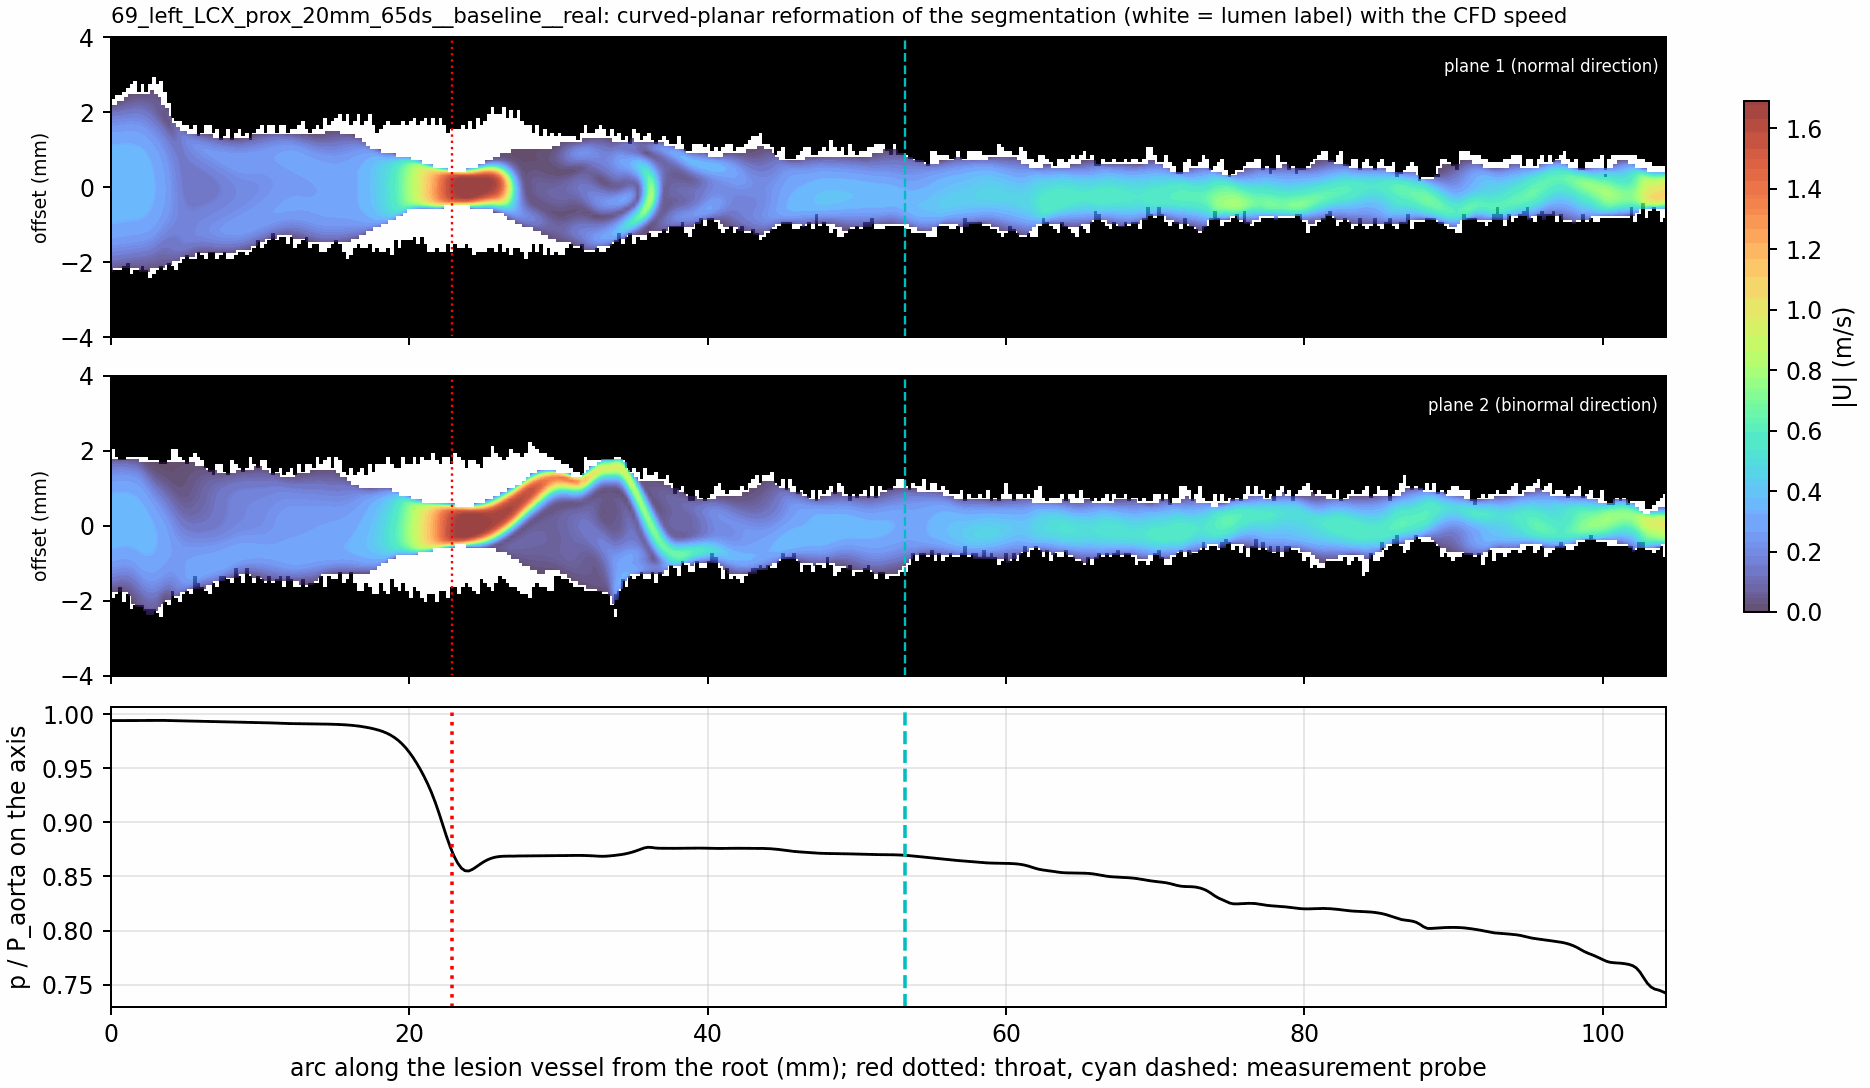
\includegraphics[width=\textwidth]{figures/cfd_p5_69_cpr_cfd.png}
\caption[P5 scan 69: segmentation reformation with the CFD speed]{P5 scan 69 (LCx, 20\,mm, 65\%DS): same layout as for scan 138.}
\end{figure}
\begin{figure}[H]
\centering
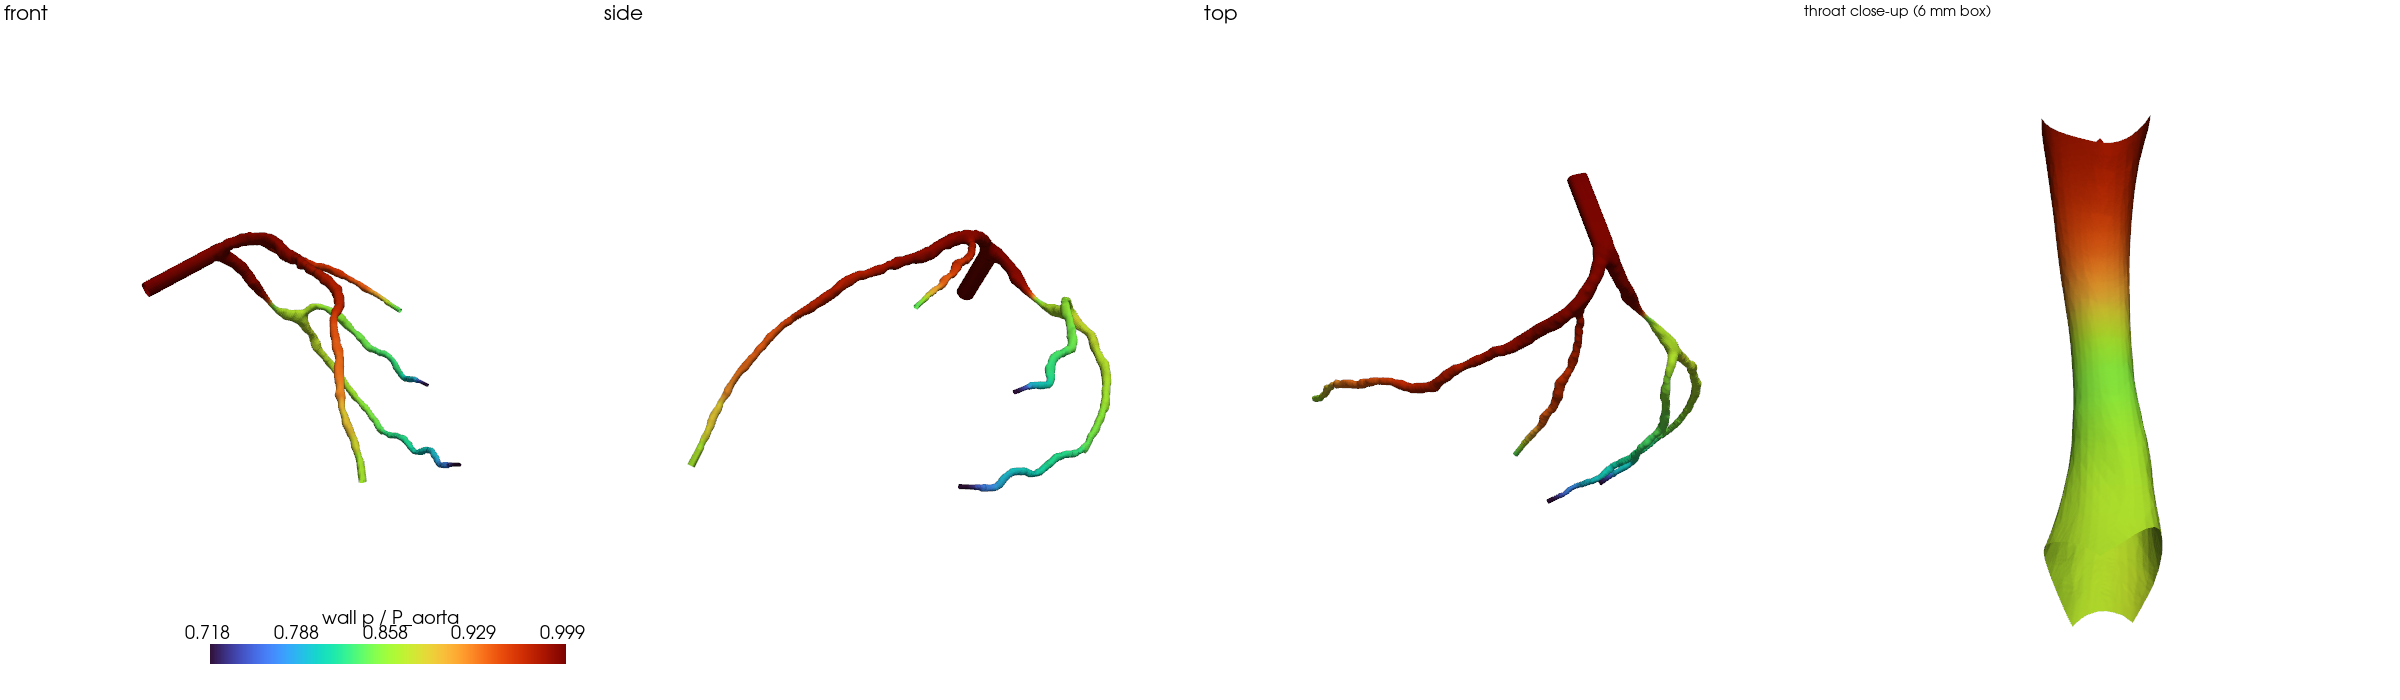
\includegraphics[width=\textwidth]{figures/cfd_p5_69_wall.png}
\caption[P5 scan 69: wall pressure]{P5 scan 69: wall pressure $p/P_\text{aorta}$ of the tree in three views and the 6\,mm around the throat.}
\end{figure}
\begin{figure}[H]
\centering
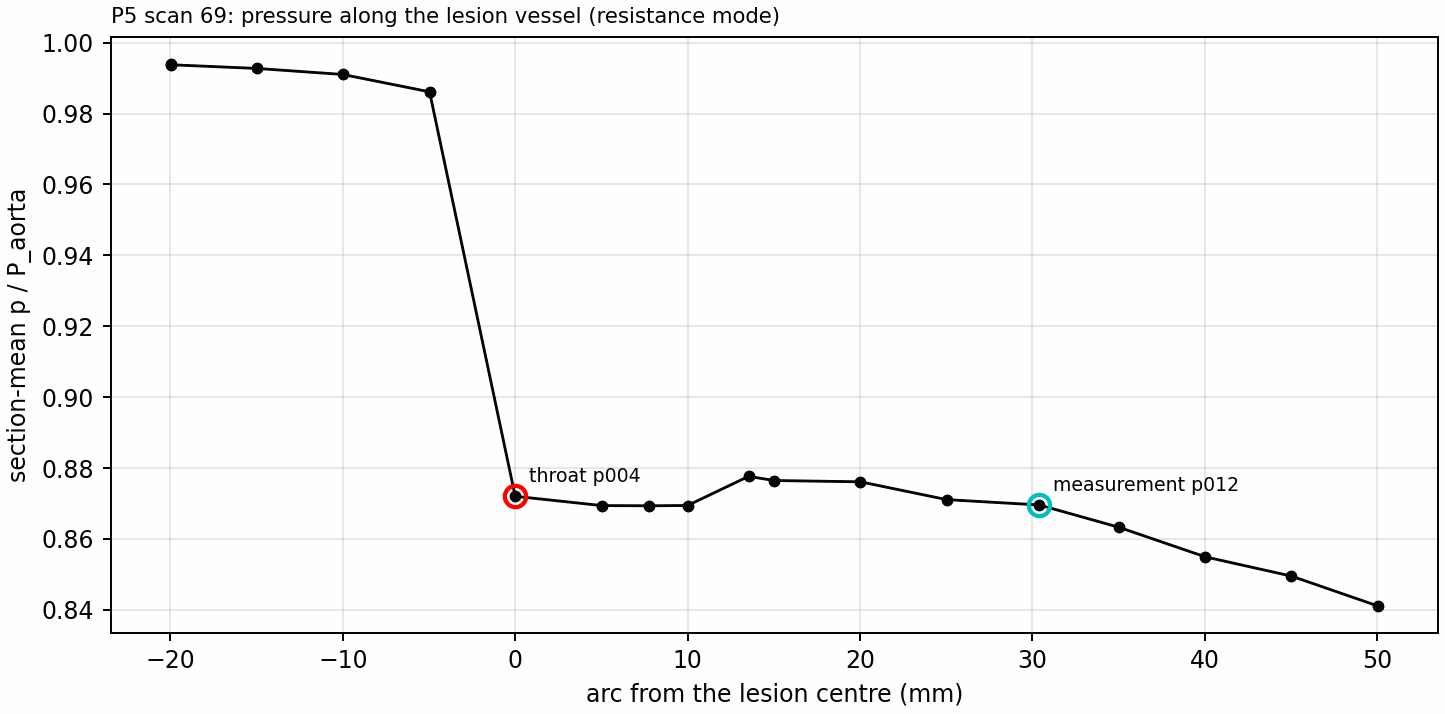
\includegraphics[width=0.85\textwidth]{figures/cfd_p5_69_profile.png}
\caption[P5 scan 69: pressure along the lesion vessel]{P5 scan 69: section-mean $p/P_\text{aorta}$ along the lesion vessel at the package probes.}
\end{figure}

\begin{figure}[H]
\centering
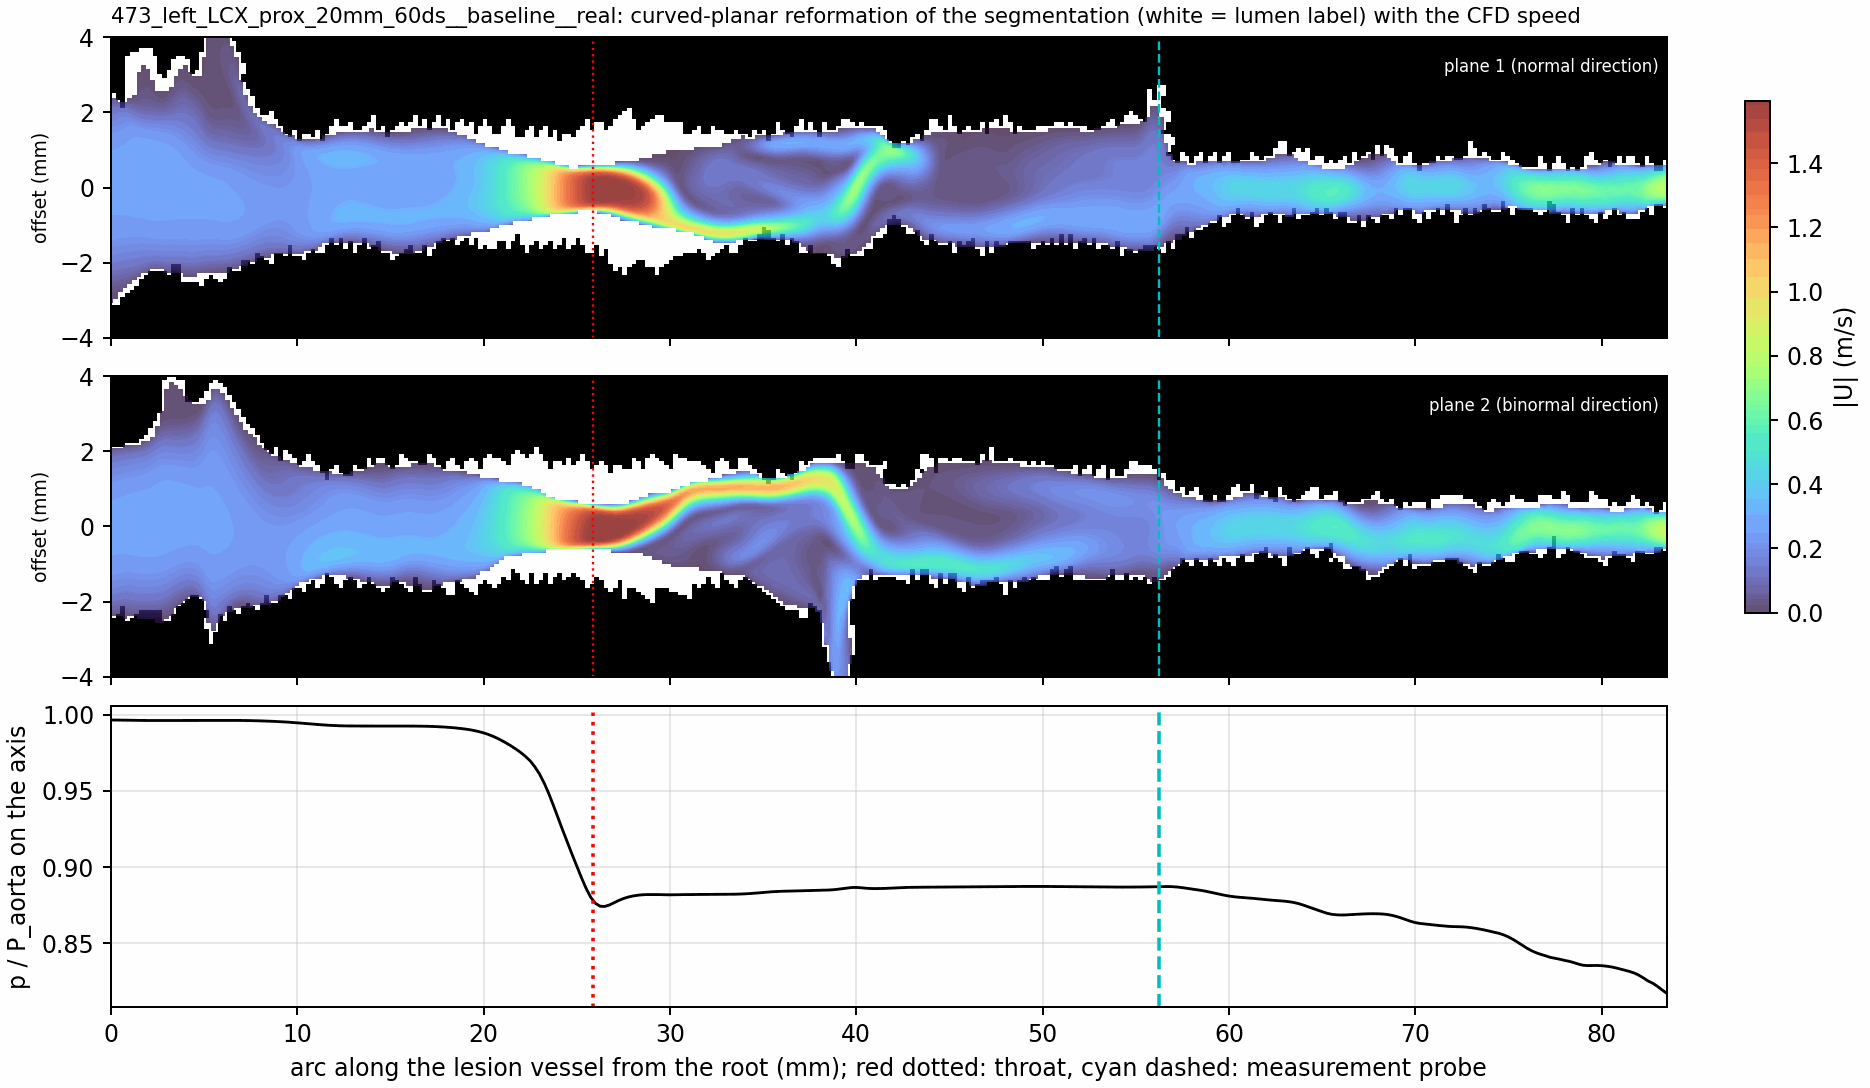
\includegraphics[width=\textwidth]{figures/cfd_p5_473_cpr_cfd.png}
\caption[P5 scan 473: segmentation reformation with the CFD speed]{P5 scan 473 (LCx, 20\,mm, 60\%DS): same layout as for scan 138.}
\end{figure}
\begin{figure}[H]
\centering
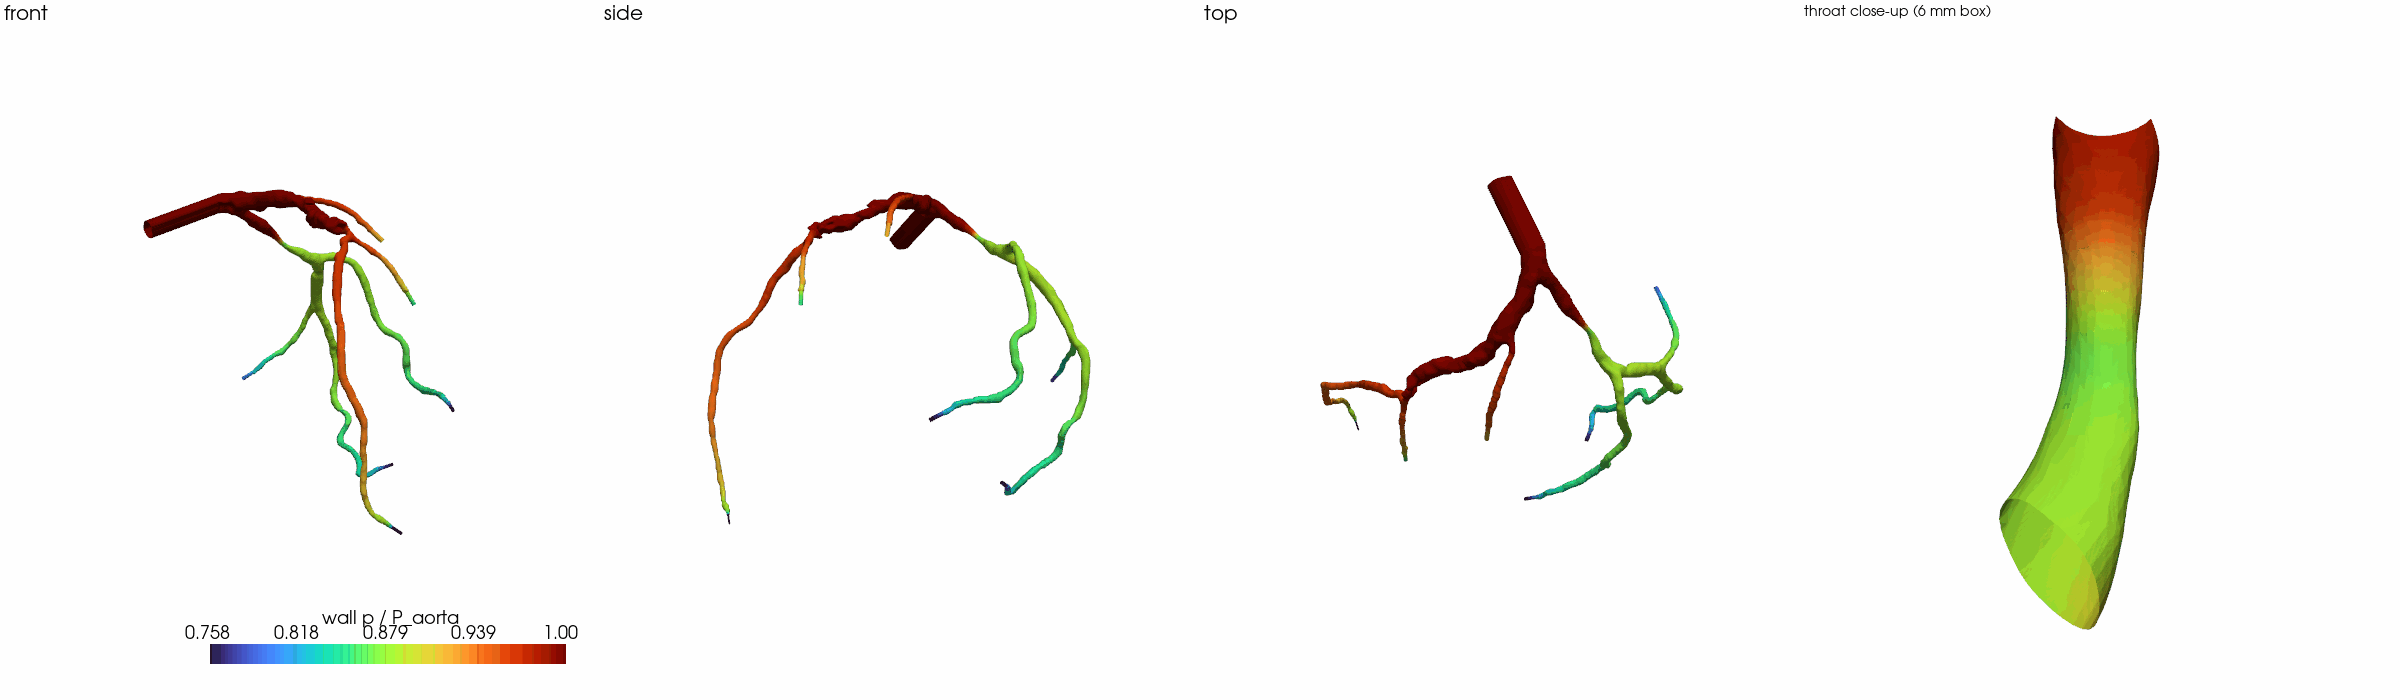
\includegraphics[width=\textwidth]{figures/cfd_p5_473_wall.png}
\caption[P5 scan 473: wall pressure]{P5 scan 473: wall pressure $p/P_\text{aorta}$ of the tree in three views and the 6\,mm around the throat.}
\end{figure}
\begin{figure}[H]
\centering
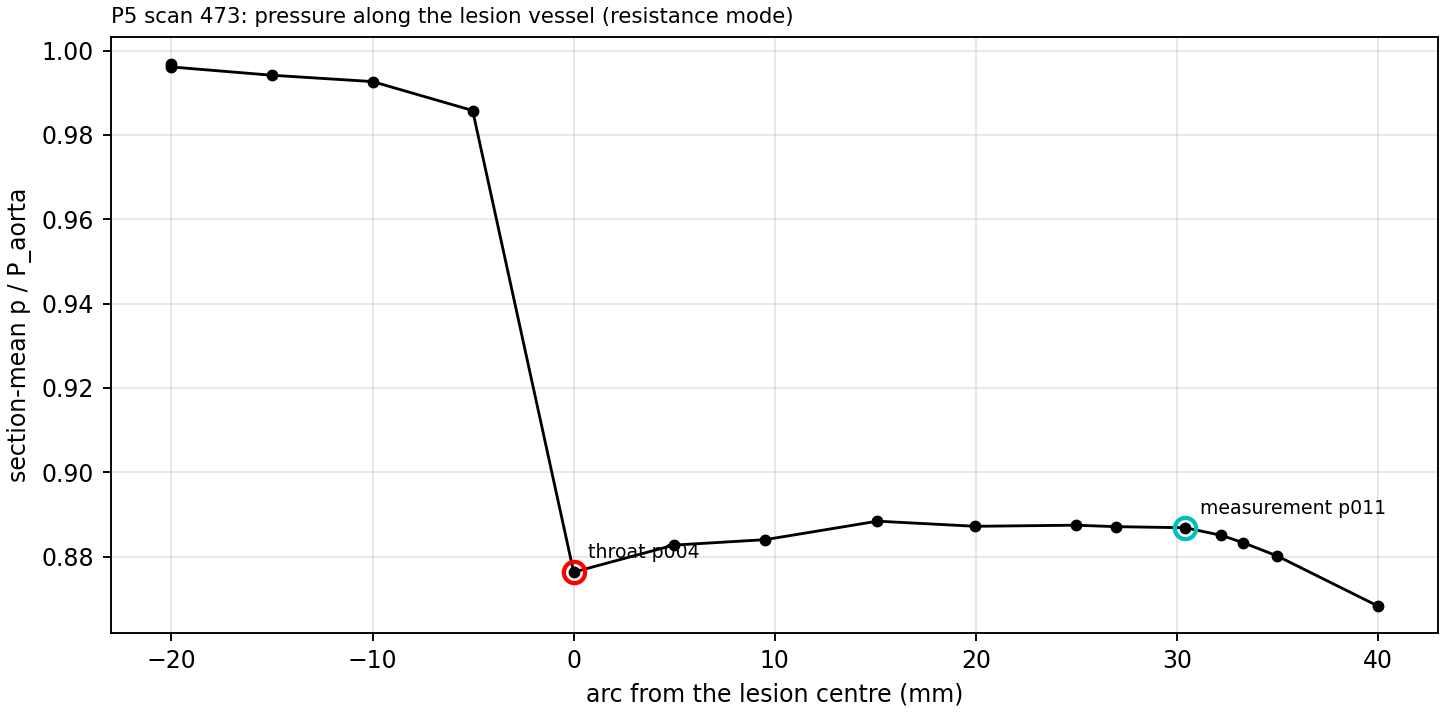
\includegraphics[width=0.85\textwidth]{figures/cfd_p5_473_profile.png}
\caption[P5 scan 473: pressure along the lesion vessel]{P5 scan 473: section-mean $p/P_\text{aorta}$ along the lesion vessel at the package probes.}
\end{figure}


\begin{figure}[H]
\centering
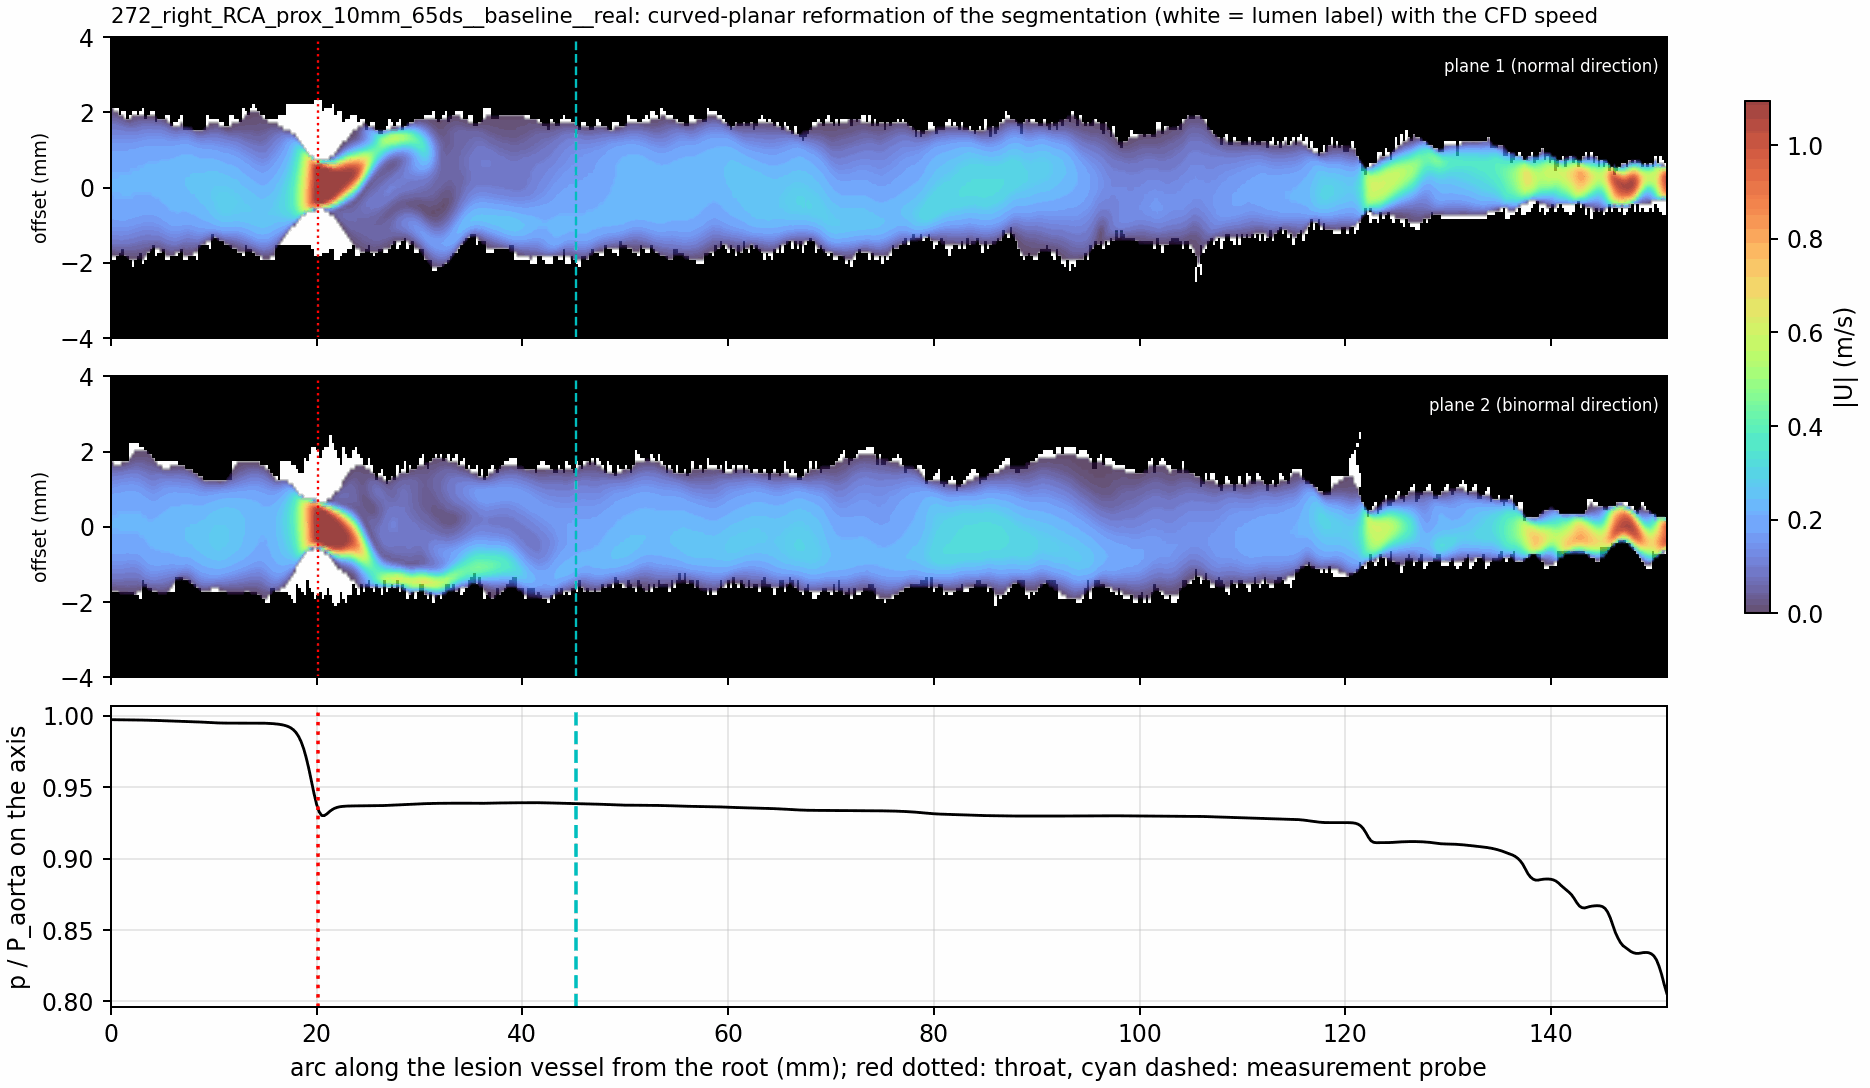
\includegraphics[width=\textwidth]{figures/cfd_p5_272_cpr_cfd.png}
\caption[P5 scan 272: segmentation reformation with the CFD speed]{P5 scan 272 (RCA, 10\,mm, 65\%DS; the outlet out\_396 was lost in the mesh and is absent from the solve): same layout as for scan 138.}
\end{figure}
\begin{figure}[H]
\centering
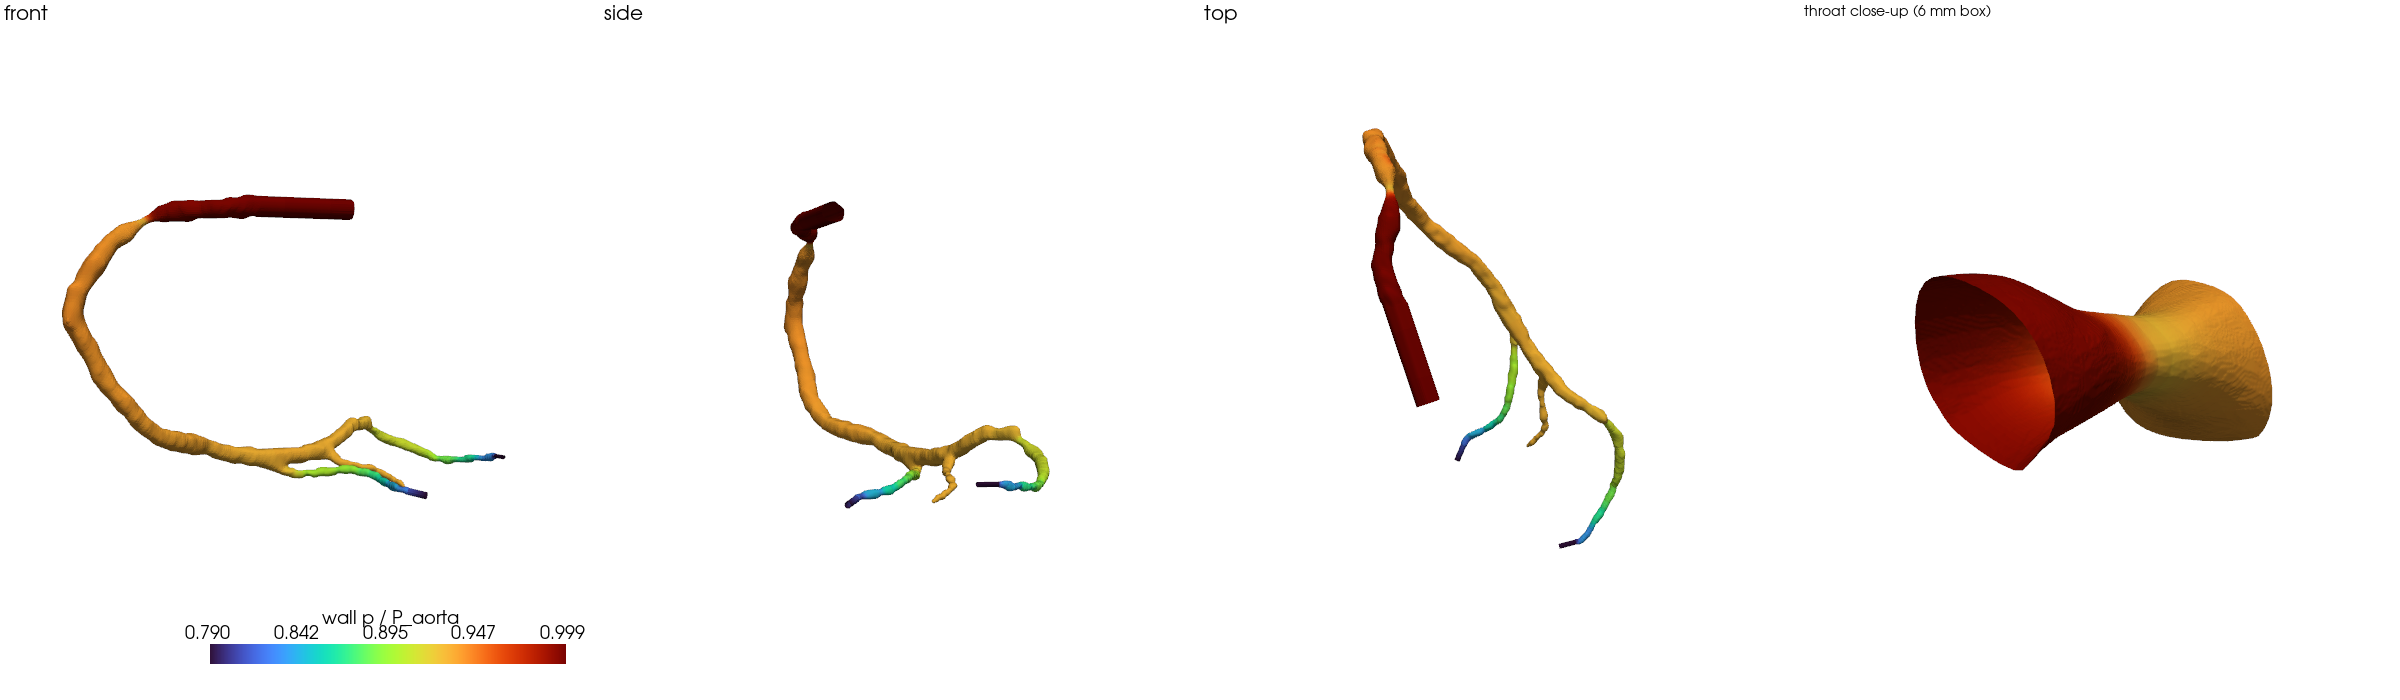
\includegraphics[width=\textwidth]{figures/cfd_p5_272_wall.png}
\caption[P5 scan 272: wall pressure]{P5 scan 272: wall pressure $p/P_\text{aorta}$ of the tree in three views and the 6\,mm around the throat.}
\end{figure}
\begin{figure}[H]
\centering
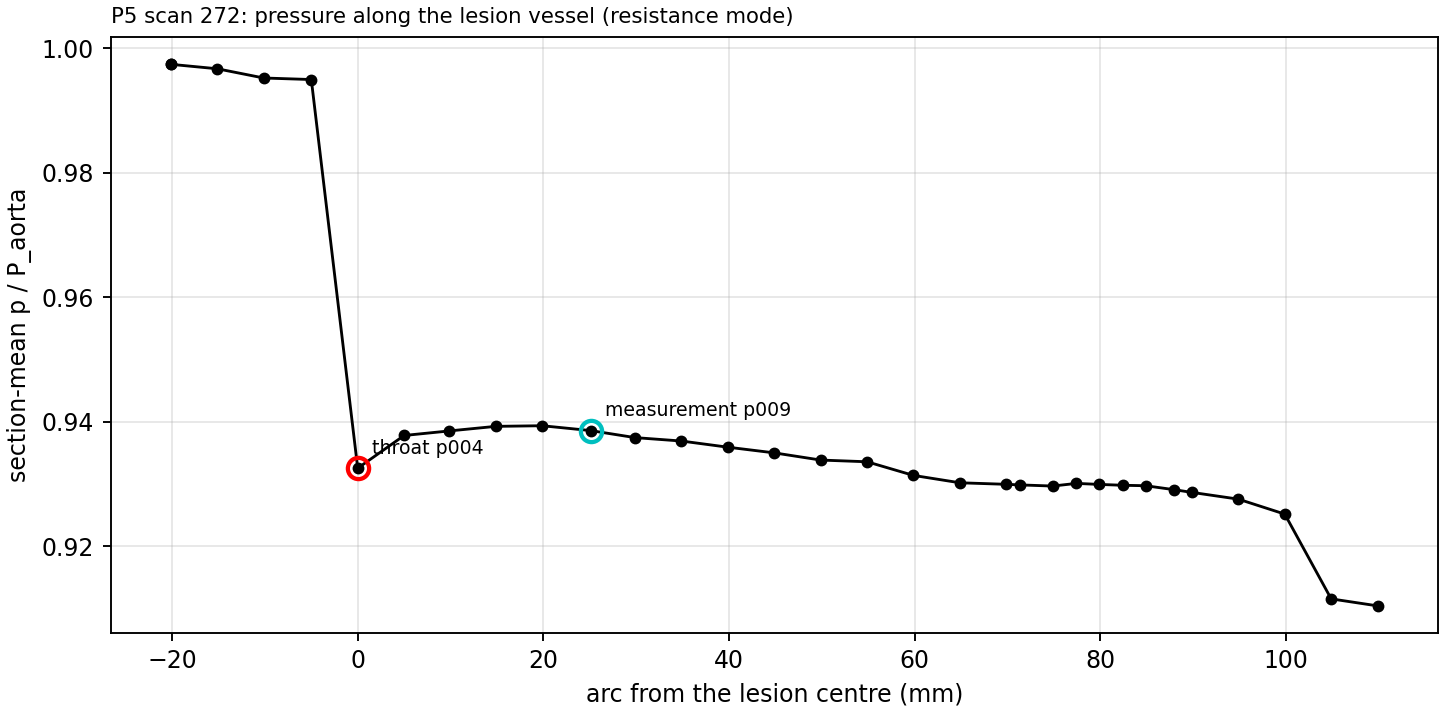
\includegraphics[width=0.85\textwidth]{figures/cfd_p5_272_profile.png}
\caption[P5 scan 272: pressure along the lesion vessel]{P5 scan 272: section-mean $p/P_\text{aorta}$ along the lesion vessel at the package probes.}
\end{figure}

\begin{figure}[H]
\centering
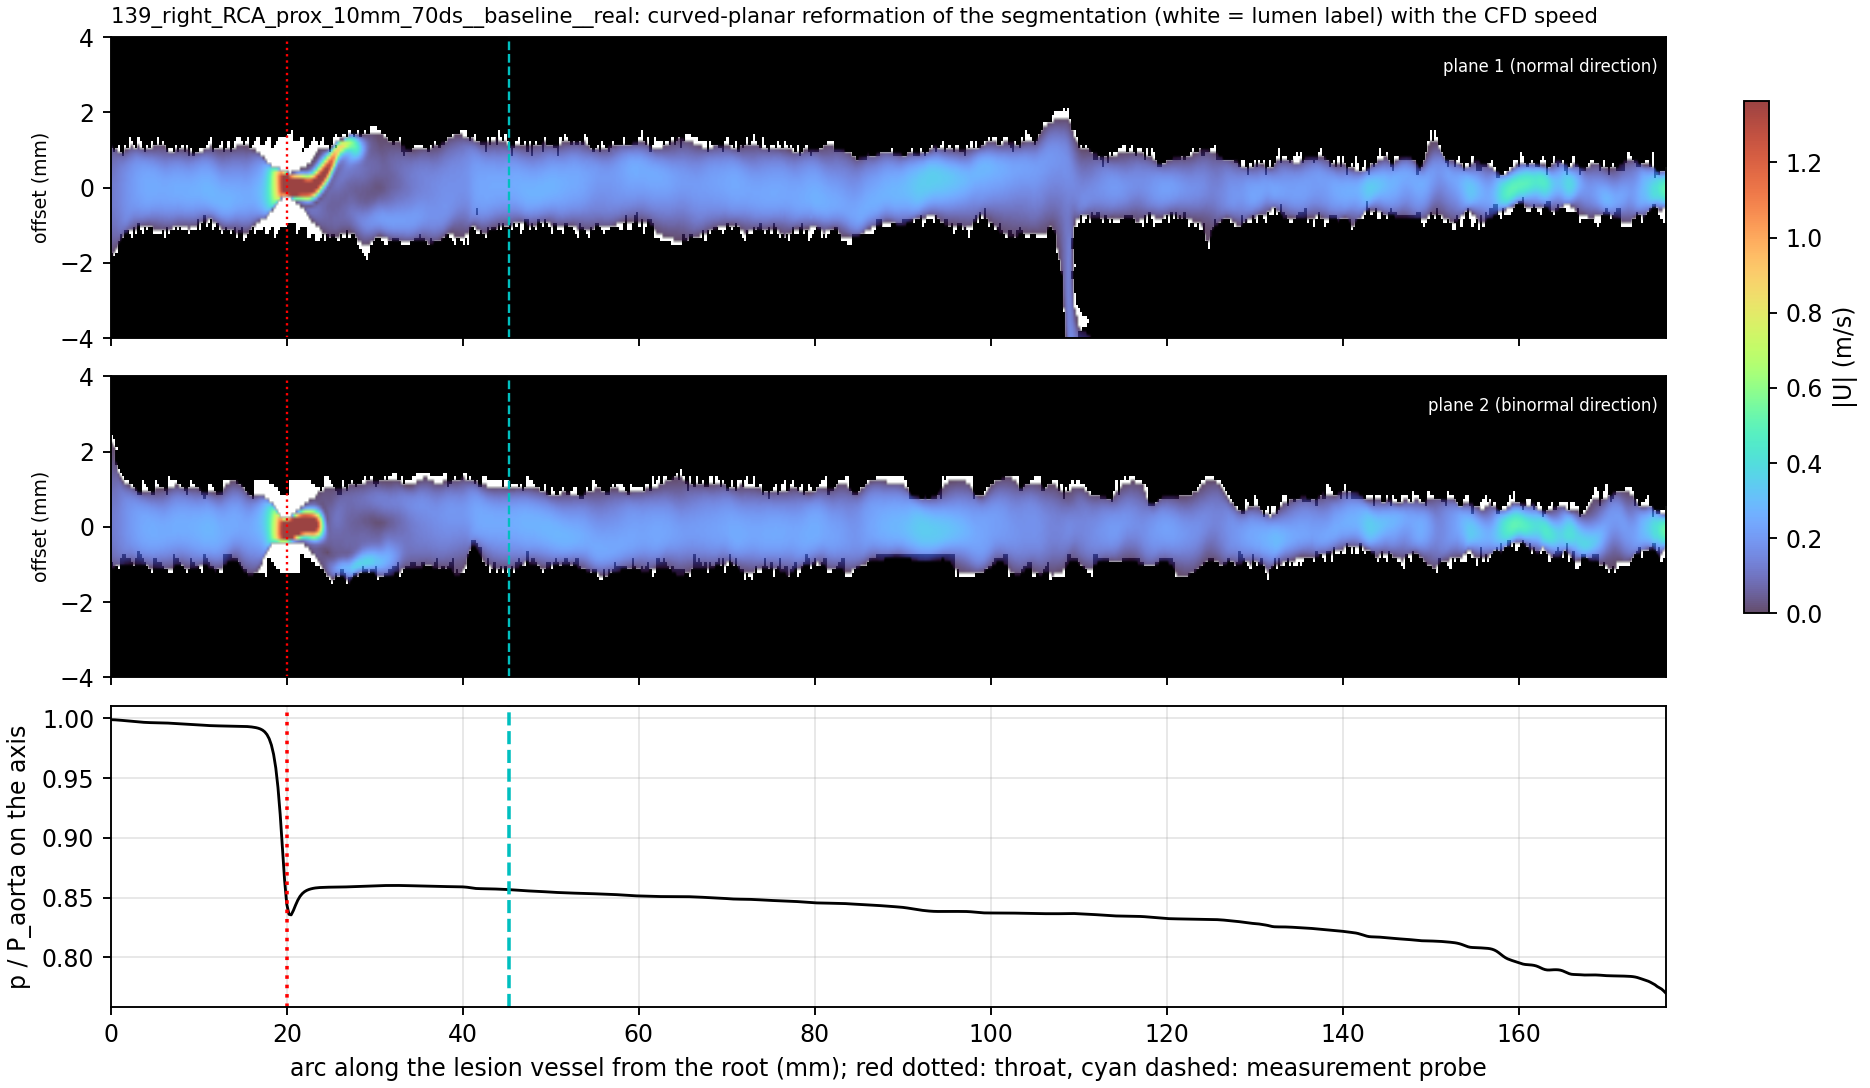
\includegraphics[width=\textwidth]{figures/cfd_p5_139_cpr_cfd.png}
\caption[P5 scan 139: segmentation reformation with the CFD speed]{P5 scan 139 (RCA, 10\,mm, 70\%DS): same layout as for scan 138.}
\end{figure}
\begin{figure}[H]
\centering
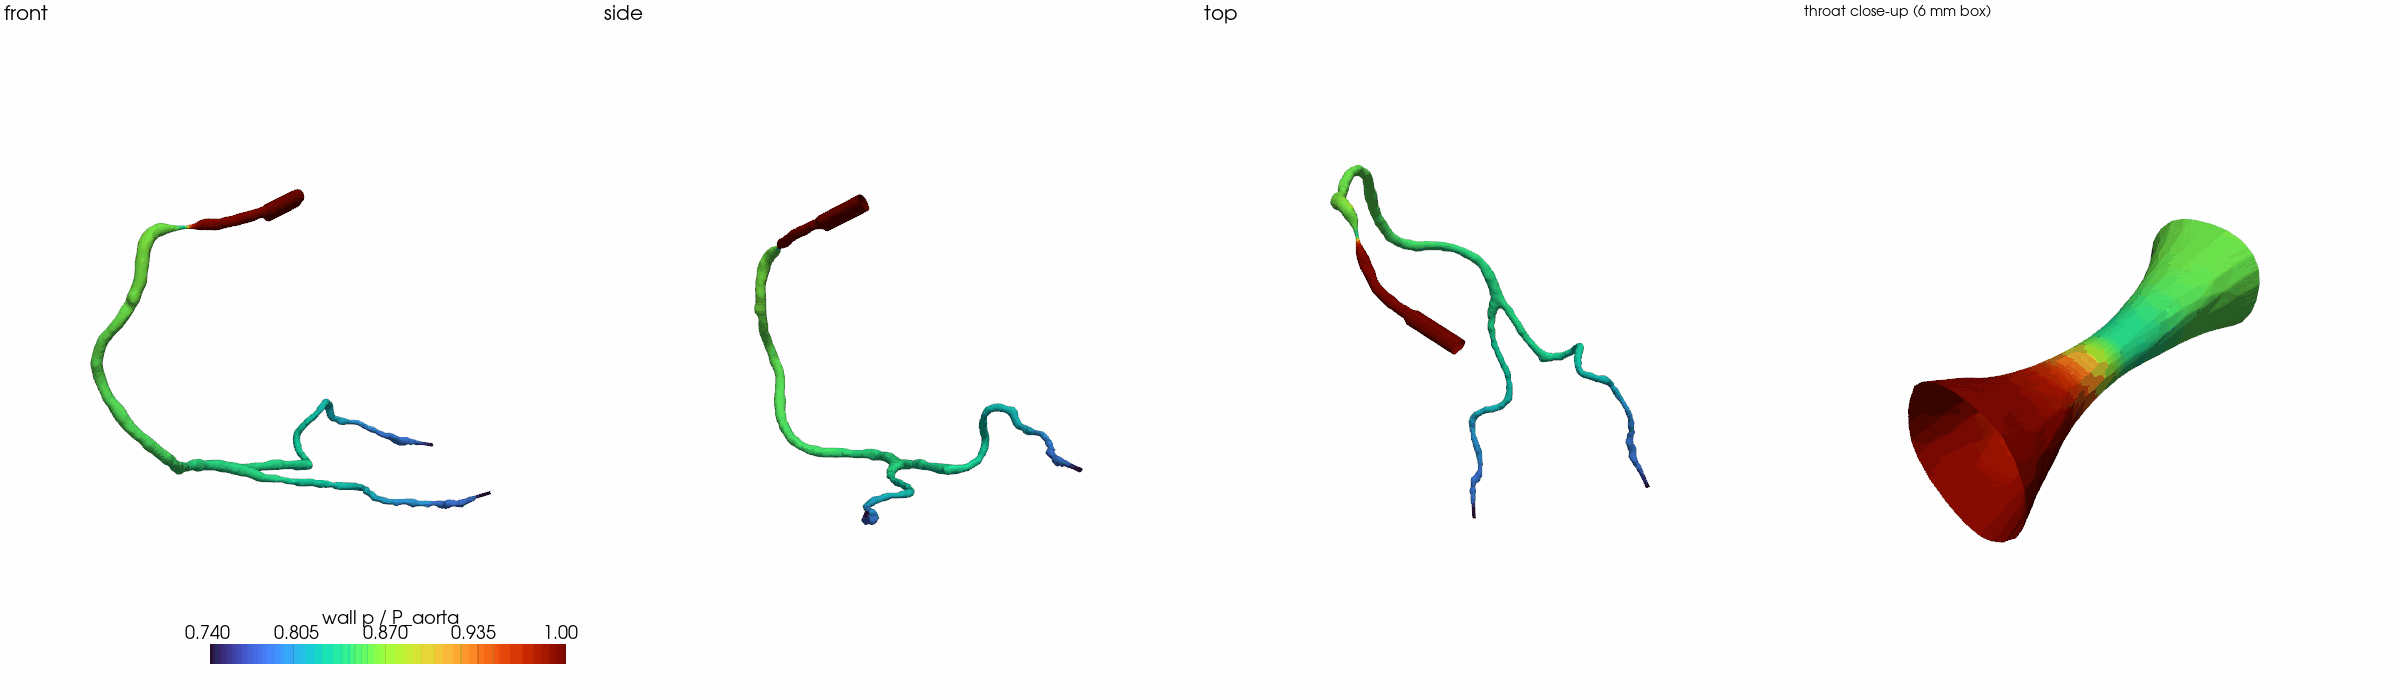
\includegraphics[width=\textwidth]{figures/cfd_p5_139_wall.png}
\caption[P5 scan 139: wall pressure]{P5 scan 139: wall pressure $p/P_\text{aorta}$ of the tree in three views and the 6\,mm around the throat.}
\end{figure}
\begin{figure}[H]
\centering
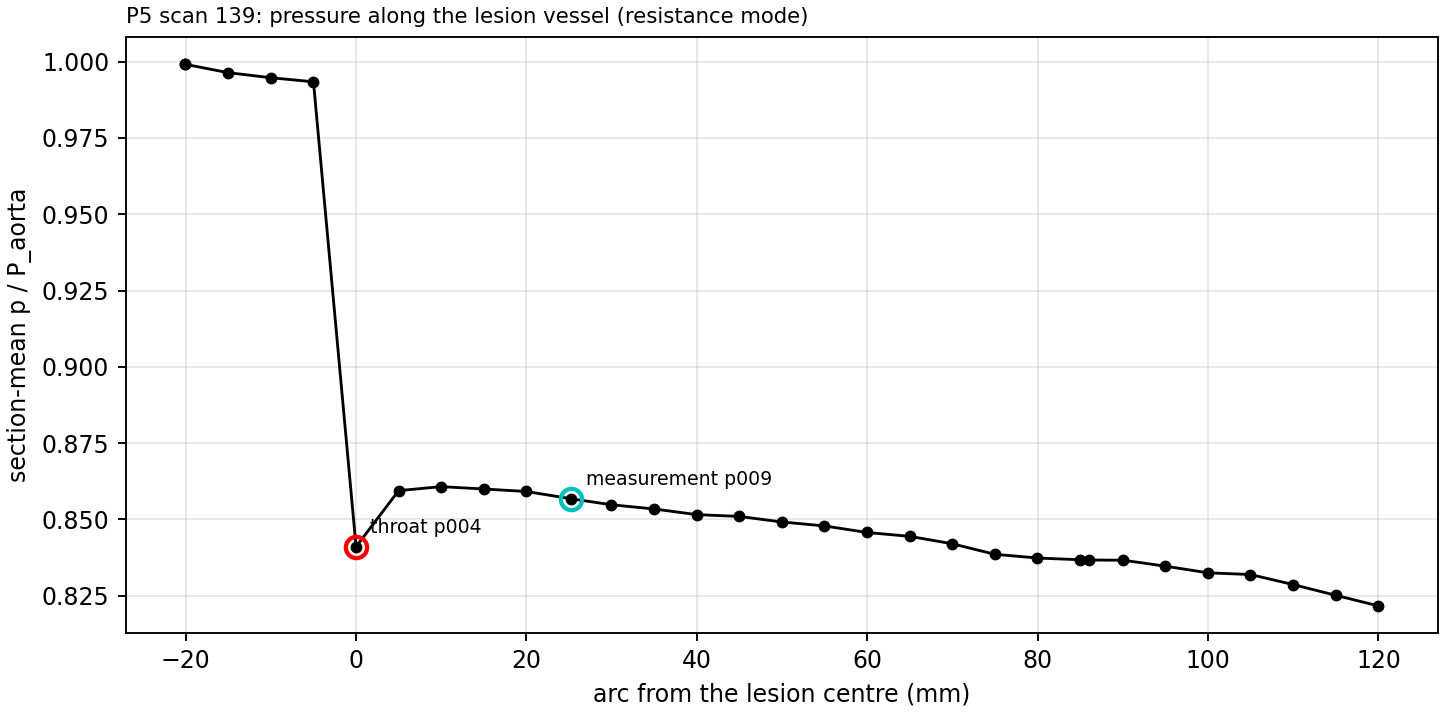
\includegraphics[width=0.85\textwidth]{figures/cfd_p5_139_profile.png}
\caption[P5 scan 139: pressure along the lesion vessel]{P5 scan 139: section-mean $p/P_\text{aorta}$ along the lesion vessel at the package probes.}
\end{figure}
%%P5_END

\paragraph{Scan 473: measurement probe (correction of 2026-10-06).} The package measurement probe p011 failed the section rule (a degree-3 node 0.84\,mm away, centreline angle 36.6$^\circ$ against 20$^\circ$ allowed) and was relocated deterministically to p011\_reloc (tree node 646, 2.85\,mm distal); the monitored and returned value is $p/P_\text{aorta}=0.88333$ there. An earlier version of Table~\ref{tab:p5} printed 0.88685, the value at the rejected package section. The D3/D4 distance of 473 (1.07\,mm) is measured to the package probe p011, not to p011\_reloc.

\paragraph{Scan 272: the lost outlet and the self-intersection flag (read-only diagnosis of 2026-10-06, revised after the post-hoc audit).}
The 272 solve is a converged solution of a \emph{truncated} domain: out\_396, which carries 0.507 of the 1.609\,mL/s package target flow (31.5\%), has no faces in the mesh. It is returned flagged as the work order requires, but it is not a reusable production baseline and should not enter a cohort comparison or the batch as it is (the decision is the analysis side's). Mechanism, consistent with every measurement but inferred in its last step: the distal R-PDA has a one-voxel neck in the mask (voxel $0.35\times0.35\times0.5$\,mm; edited-mask EDT radius 0.35--0.49\,mm at tree nodes 379--382, 6.4\,mm upstream of the outlet) that the marching-cubes surface already narrows (area-equivalent radius 0.339\,mm at node 381) and the Taubin smoothing of the recipe narrows further (0.278\,mm, $-18\%$; inscribed radius 0.228\,mm); none of the 104 refinement objects covers nodes 378--383 (parsed from the mesh dictionary; the 100\,$\mu$m cones follow the lesion path only and the out\_396 cap sphere is 9.6\,mm away), so cfMesh meshes the neck with its 200\,$\mu$m root cells, 2.3 cells across the inscribed diameter; the mesher reports two unconnected regions and deletes the smaller one (32{,}527 cells). That the deleted region is the distal R-PDA beyond this neck is inferred, not localised against the mesh boundary. The build note's ``100\,$\mu$m background'' at the neck is corrected to 200\,$\mu$m. From one case no general threshold follows; as a risk, a non-lesion branch that narrows to a few root cells between the lesion path and an outlet may lose that outlet the same way (the patch gate catches it; a recipe change is for the analysis side). The single location that \texttt{surfaceCheck} reports on the inlet flow extension (5.1\,mm upstream of the inlet plane) shows no geometric intersection or contact in a triangle--triangle distance check of all 2{,}930 triangles within 3\,mm (minimum distance between non-adjacent triangles 4.85\,$\mu$m, the width of a sliver column 0.6\,mm away; no fold-over), \texttt{surfaceCheck} on that 3\,mm sub-surface reports none, and on larger sub-surfaces it reports other locations, where the same check again finds none. This is consistent with a tolerance artefact of the tool, but not proven; the flag stays as returned, because the gate is defined by the tool's verdict. Files: \texttt{returns/2026-10-03/P5/272/ROOT\_CAUSE\_272\_2026-10-06.md} and the evidence beside it, scripts in \texttt{code\_\allowbreak{}from\_\allowbreak{}cfd/\allowbreak{}task\_\allowbreak{}1003/\allowbreak{}p5\_\allowbreak{}diagnostics}.

\subsection{Item 5: RCR outlet BC verification --- \PASS{}}
\label{sec:item5-status}
The Crank-Nicolson coded RCR BC (\S\ref{sec:item1}'s design revision, independently verified standalone
against scipy to 0.011\% at a 10\,ms timestep before ever compiling in OpenFOAM) was run on Stage A's
pipe geometry (61,440 cells, PIMPLE, adjustable timestep targeting the stated Courant limit) for 2 full
pulsatile cycles (2\,s), reaching $t=2.0000$\,s cleanly with no errors, 17,316 timesteps, mean Courant
0.044 (max 0.52, at the 0.5 target). \textbf{Independently re-run by the coordinator, not just taken
from the fork's report}: comparing the solver's own outlet-pressure monitor against a from-scratch scipy
RK45 integration of the same RCR ODE (same $R_1,R_2,C,P_v$, same prescribed $Q(t)$, same $p_C(0)=0$
initial condition) over the second cycle only gives a \textbf{maximum relative error of 0.2827\%} (mean
0.042\%) --- comfortably under the 0.5\% pass criterion, using 56\% of the tolerance budget (the error is normalised by the maximum $|p_\text{ref}|$ over cycle 2, as the pre-registered metric defines it; the point-wise relative error peaks at 0.54\% at $t=1.911$\,s, found by the post-hoc audit). No
NaN/blow-up/growing oscillation occurs during the backflow window (1,195 of 8,656 cycle-2 samples have
$Q<0$; pressure stays smooth and bounded, 250--4420\,Pa throughout, and the worst-case error itself
occurs during backflow without escalating). A mass-conservation sanity check (outlet flux vs.\ the
prescribed inlet $Q(t)$ through the rigid pipe, independent of the outlet BC) agrees to 0.25\%.

\textbf{Operational note:} a stale 7-line file from an earlier serial compile-smoke-test (run first,
deliberately, to force the coded BC to compile before the parallel launch --- the same MPI
recompilation-race precaution Item 4's design calls for) sat at the same \texttt{postProcessing} path
the real run also wrote to; OpenFOAM avoided clobbering it by suffixing the real run's file
(\texttt{\_\allowbreak{}0}), and the first comparison attempt's file glob picked up the stale stub instead, producing
an empty cycle-2 array. Caught immediately (an empty array is a loud failure, not a silent wrong
answer) and fixed by globbing for the largest matching file rather than an exact name.

\subsection{Operational incident: cross-fork CPU oversubscription, diagnosed and fixed}
\label{sec:contention}
While Items 1, 2, 3+4, 5 and 6 ran in parallel (three background subagents plus this document's own
coordinator process), the machine became severely oversubscribed: load average reached 78 with 48
concurrent OpenFOAM solver processes. Per this document's standing practice, a three-reviewer panel
(Fable~5.1, GPT-6-astra, Gemini~3.8~Flash) was convened on the live problem itself, not just on CFD
setups. Two of three reviewers independently confirmed, by reading each \texttt{mpirun}'s working
directory and \texttt{/\allowbreak{}proc} state directly rather than trusting the coordinator's own attribution, two
facts the coordinator had gotten wrong: (i) a group of three solves the coordinator had attributed to
the Item 3+4 fork actually belonged to Item 2 (which had launched sten60, sten65, and sten70's 4th mesh
level concurrently rather than sequentially); (ii) the host has 16 physical cores, not the 32 logical
threads \texttt{nproc} reports --- CFD's memory-bandwidth-bound solvers gain little from SMT, so the
true available budget was roughly 8 free physical cores, not the $\sim$24 assumed when each fork was
given its own core guidance in isolation. All three reviewers independently identified Open MPI's
default non-yielding busy-wait behaviour (each \texttt{mpirun} perceives itself as undersubscribed
against the 32-thread host and spins rather than yields) as amplifying the effective slowdown to
roughly 5$\times$, well beyond the naive 1.5$\times$ the raw process-count ratio would suggest --- one
reviewer measured this directly (wall-time-per-step degrading from $\sim$8\,s uncontended to
$\sim$45\,s contended on the same case).

The panel's fix was applied in full: Item 6's two pulsatile runs were stopped (their deliverable, a
wall-clock cost estimate, had already been captured from a smoke test --- later found to have run alongside other solves, hence contended, see \S\ref{sec:item6} --- so no further Item~6 result was lost); Item 2's sten60/sten65 solves were stopped (already fully
converged and reported, so continuing to run them to their nominal end iteration was pure waste); the
Item 3+4 fork was instructed to run its remaining solves strictly sequentially rather than concurrently
before launching any of them. All four stops used OpenFOAM's own graceful \texttt{stopAt writeNow}
mechanism, not a hard kill. Load fell from 78 to 33 within a minute of the fix, and the remaining
solves (Item 1, Item 5, Item 2's sten70 4th level) measurably accelerated. No result's correctness is
affected --- convergence is independent of wall-clock pacing --- but this incident is exactly why Item
6's own wall-clock numbers are reported from the smoke test (itself contended, see \S\ref{sec:item6}) rather than the fully contended
runs, and it is disclosed here in full rather than folded silently into the numbers, consistent with
this document's practice for every other incident in this study.

\section{Conclusions}
\textbf{Stage A.} Of the seven pass/fail rows of the running summary (\S\ref{sec:summary}), six pass and one is not established. A1, A3 on sten00 and sten50, and A4 are clean, unanimous passes; A3 on sten80 is a flagged pass (numeric tolerance met, the stricter residual criterion not, cause left open between a numerical SIMPLE stall and a slow physical instability; a time-accurate diagnostic was scoped, reviewed and deliberately not run once its cost was weighed against a free check showing the practical effect on FFR to be inside the study's accepted tolerance, \S\ref{sec:pimple}); A5 on sten80 passes comfortably, with the new observation that the fluctuation band grows with refinement (mild evidence against a pure numerical-stall origin). \textbf{A5 on sten70 is NOT ESTABLISHED}: it met its numeric tolerance at 94.6\% of the budget with a non-monotone sequence, and the fourth level of Item 2 did not confirm a convergent trend; the Celik--Eça--Hoekstra analysis is not trustworthy there because the boundary-layer stack was held constant across levels (\S\ref{sec:item2}). A2 is informational by design and shows the 0D-vs-3D gap growing and changing sign with severity ($-3.01\%$ at 0\%DS, $-1.48\%$ at 50\%DS, $+8.68\%$ at 80\%DS). The coded resistance-outlet BC, the central risk of the audit-and-fix effort, is confirmed on four straight-vessel geometries (sten80 flagged), an idealised 3-outlet tree and a real 5-outlet coronary tree (scan 837); the prescribed-flow mode, run first on a single outlet (A4), now also closes its round trip on the 3-outlet Item 1 tree at both severities (all outlets prescribed together, largest flow error $0.0007\%$), and on the six-outlet real lumen of scan 14 (three cases, largest flow error $0.0051\%$; \S\ref{sec:m1}).

\textbf{Beyond Stage A.} Item 1: the idealised branched tree with the automatic relaxation rule gives outlet flows within 1.04\% of the 0D twin (both severities) and BC errors below $2\times10^{-4}\%$. Item 2: the four-level ladder of \S\ref{sec:item2} did not give a trustworthy 3D discretisation uncertainty for sten70; the systematic family of \S\ref{sec:u3d} gives $U_{3D}=0.00055$, provisional because the case has two stable steady states and the state of each level was not recorded (\S\ref{sec:b3}; levels S50, S25A and S25B have since been verified to be on the axisymmetric state); the severity sweep brackets the sign change of the 0D-vs-3D flow gap between 50 and 60\%DS. Items 3 and 4: the meshing blocker of the real-lumen pipeline was root-caused (the surface remesh pinched narrow lumens) and removed; the rebuilt pipeline yields converged 5-outlet solves; for the lesion80 case of scan 837 the ten registered quantities are insensitive to the throat mesh (W100, M50, T25a, T25b), to an extension of the refined tube (Table~\ref{tab:e60}), and the hyperaemic pair (\S\ref{sec:followup}) shows a 3D flow reduction smaller than both 0D variants at $3.16\times$ the flow, with the recirculation extent beyond arc 34\,mm not mesh-supported. Task 1: the 3D FFR discretisation uncertainty of sten70 from a systematic refinement family is $U_{3D}=0.00055$ (\S\ref{sec:u3d}), a pre-registered PASS (accepted by the analysis side, decision D1, which fixes the scan-14 mesh recipe as the production recipe). Task 3: the scan-14 pipeline is scripted end to end without manual repair, all solves converge, both boundary-condition modes are stable and the three round trips close to $\leq0.0051\%$; against the decisions D2--D4 the relative throat gate passes, the clean case meets the 2\,mm rule for flagged mesh entities and the two lesion meshes do not (faces with poorly decomposing tets 1.43\,mm from the throat), so those two cases fail M1 as stated and are reported, not repaired (\S\ref{sec:m1}); the E0 assertion for scan 14 passed against the shipped frozen-subset file. Item 5: the RCR boundary condition passes. Item 6: the pulsatile runs were stopped; only a cost estimate exists. \textbf{Scan 837 is a pipeline pilot outside the frozen cohort; none of this is a Gate M1 result.}

\textbf{Open items (not run or not finished at the time of writing).} (i) Task~1: the wedge cross-check is complete; a jet-symmetry check of the 3D levels is needed before $U_{3D}$ is final: all five levels S50 to S12B are verified axisymmetric (2026-10-02 to 2026-10-05, \S\ref{sec:taskB}). Task~B3 is complete: the smoke test accepts either steady state and was passed on both by two fresh runs (\S\ref{sec:b3}). (ii) Gate M1 on the shipped scan-14 packages (\S\ref{sec:m1}): the geometry, meshes, the three resistance-mode solves and the prescribed-flow solves with round trips of all three cases are done. The surfaces fail the self-intersection gate and the literal absolute throat check (reported as results; D2/D3), the two lesion meshes fail the 2\,mm rule of D4 (reported; the verdict rests with the analysis side), and the E0 assertion passed on 2026-09-26 against the shipped subset file (D5). (iii) Task~B2 was measured on 2026-10-01 (\S\ref{sec:b2}): one 16-rank job gave about 7\% more solves per hour than two 8-rank jobs, but both layouts failed the strict isolation rule (short peaks of operating-system updates and of the coordinating session), so the ratio is not claimed; a replicate on a quiet host is open. The uncontended pulsatile timing of the earlier Task~4 (tooling audited four times, the last audit by GPT-5.6 Sol still NOT READY for evidence-validation hardening; run not made, and not part of the work order of 2026-09-26, whose Task~B2 replaces the need for an uncontended timing): see the note of the returns folder for their status. (iv) The mesh sensitivity of the hyperaemic case, the isolated-lesion and transient-steadiness checks, which were built and audited but not run because the work order closed new work on scan 837. (v) The sten80 numerical-versus-physical question. (vi) Audit coverage: while this report was being finalised the GPT-6 Astra auditor reached its usage limit (until 2026-09-26 18:22); by the study's rule no new CFD setup runs before it has been audited by both auditors, so nothing new was started in that window. Its quota returned at 18:31 and it audited Tasks 1, 0, 3 and 4 in that order (all done; Task 4 was not ready). \emph{Audits of the returns and setups of the work order of 2026-09-26} (Gemini~3.8 Flash and GPT-5.6 Sol, which replaced GPT-6 Astra as the codex auditor at the study lead's instruction): numbers audit Gemini sound with caveats and Sol defects (incorporated: the settle-iteration table is labelled a proxy, not B1 as specified; the meaning of \texttt{covered} in the as-meshed radius files is stated; 12 versus 56 flagged vertices clarified; stale notes and statements corrected); B2 and B3 pre-run audits ready with conditions from both auditors, conditions fixed by Opus~5.5 (attempts 1 to 2 of the defect protocol), a delta audit pending at the time of writing.

The sten80 episode is also a demonstration of the review discipline this document has followed
throughout: reviewers were asked before hardware time was spent, not after; a specific, checkable
claim (Fable's sten70 comparison) was independently verified against this document's own logs rather
than trusted on authority; two reviewers caught the same fatal bugs by independently reading the same
source code, which is why the fix could be trusted; and when the reviewers' own recommendation turned
out to cost far more than estimated, they were brought back and re-consulted rather than the plan
being quietly abandoned or quietly pushed through. Gemini 3.8~Flash's unavailability for the last two
rounds (7 failed attempts, a Google-side OAuth/DNS issue) is disclosed rather than papered over; the
2-of-3 panel that remained still reached a defensible, well-evidenced joint recommendation.

\end{document}
